\documentclass[12pt, openright, oneside, a4paper, brazil]{article}

% Pacotes básicos
\usepackage[utf8]{inputenc}
\usepackage[left=3cm,top=3cm,right=2cm,bottom=2cm]{geometry}
\usepackage{setspace}
\setlength\parindent{1.25cm}
\usepackage{graphicx}
\usepackage{xcolor}
\usepackage{color}
\usepackage{listings}
\usepackage{microtype}
\usepackage{float}
\emergencystretch=3em
\usepackage{listingsutf8}
\lstset{
	basicstyle=\ttfamily,
	columns=fullflexible,
	frame=single,
	breaklines=true,
	showstringspaces=false,
	postbreak=\mbox{\textcolor{red}{$\hookrightarrow$}\space},
	inputencoding=utf8,
	extendedchars=true,
	literate=
	{á}{{\'a}}1
	{é}{{\'e}}1
	{í}{{\'i}}1
	{ó}{{\'o}}1
	{ú}{{\'u}}1
	{ã}{{\~a}}1
	{õ}{{\~o}}1
	{â}{{\^a}}1
	{ê}{{\^e}}1
	{ô}{{\^o}}1
	{ç}{{\c c}}1
	{Á}{{\'A}}1
	{É}{{\'E}}1
	{Í}{{\'I}}1
	{Ó}{{\'O}}1
	{Ú}{{\'U}}1
	{Ã}{{\~A}}1
	{Õ}{{\~O}}1
	{Â}{{\^A}}1
	{Ê}{{\^E}}1
	{Ô}{{\^O}}1
	{Ç}{{\c C}}1
}

\renewcommand{\figurename}{Figura}

% Variáveis
\newcommand{\subtUm}{CONTEXTO}
\newcommand{\subtDois}{RESULTADOS E EXPLICAÇÕES}
\newcommand{\subtTres}{CÓDIGOS}

\begin{document}
	
	\begin{center}
		\thispagestyle{empty}
		\textbf{\uppercase{Universidade Federal do Rio Grande do Norte}}\\
		\textbf{\uppercase{Bacharelado em Tecnologia da Informação}}\\
		\vspace{4cm}
		AKIRA VITOR DE LIMA YAMAZAKI\\
		\vspace{5cm}
		\textbf{RELATÓRIO DA UNIDADE 2}\\
		Computação de Alta Performance\\
		\vspace{11cm}
		NATAL, RN\\
		2026\\
	\end{center}
	
	\newpage
	\onehalfspacing
	\section{TAREFA 10}
	\subsection{\subtUm}
	\par{Avaliar a arquitetura do computador pessoal e identificar possibilidades de paralelismo disponíveis. Com base nessa análise, analisar quais estratégias de paralelismo podem triar mais proveito desse ambiente.
		
		Em seguida, realizar a mesma análise no supercomputador do NPAD.}
	\subsection{\subtDois}
	\par{Modelo: Lenovo ThinkPad X270
		Processador: Intel Core i5-7300U 4 threads
		Memória: 8GB RAM
		GPU: Intel HD Gaphics 620 (KBL GT2)
		SO: Fedora Linux 44
		
		Conta com arquitetura de multiprocessadores, com dois núcleos que permitem o compartilhamento de algum nível de memória cache e a memória principal, permitindo o programador coordernar o paralelismo em seu programa.
		Em questão de aceleradores, possui uma GPU integrada.
		Pela classificação de flynn, a CPU se encaixa como MIMD, em que que cada core pode executar instruções diferentes de forma independente, sobre dados independentes. Enquanto a GPU usa estrutura SIMD, com uma única instrução operando sobre diversos dados diferentes.
		A GPU utiliza a arquitetura gráfica Intel Gen9.5, associada à plataforma Kaby Lake (KBL GT2).
		Para essa máquina, a estratégia mais adequada é explorar paralelismo em threads e em instruções na CPU, e paralelismo de dados na GPU quando o problema tiver operações massivamente paralelas. O paralelismo entre processos também pode ser usado, mas tende a ter um custo maior de memória e comunicação.
		
		O NPAD é um cluster heterogêneo de memória distribuída: um conjunto de nós independentes, cada um com sua própria memória, ligados por redes InfiniBand e gerenciados pelo escalonador SLURM. O sistema se enquadra como um MIMD de memória distribuída. Cada nó, por sua vez, é um multiprocessador MIMD de memória compartilhada com dois soquetes, ou seja, com acesso não uniforme à memória (NUMA). Os nós de CPU vão de 2 Xeon E5-2698v3 (32 núcleos, nas partições intel) a 2 EPYC 7713 (128 núcleos, na amd-512) e 2 EPYC 9654 (192 núcleos e 3TB de memória, na amd-3tb), com instruções vetoriais AVX2 ou AVX-512. Como aceleradores, há GPUs NVIDIA V100, A100, H100 e H200, de 4 a 8 por nó, e FPGAs Alveo U50. O armazenamento usa o sistema de arquivos paralelo BeeGFS.
		
		Com isso, é possível explorar paralelismo em vários níveis: vetorização em cada núcleo, threads dentro do nó, processos entre os nós e paralelismo de dados massivo nas GPUs. A estratégia mais adequada é a híbrida: MPI entre os nós e OpenMP dentro de cada nó, com afinidade de threads para respeitar a organização NUMA. Nas GPUs, usa-se CUDA ou OpenMP offloading, com um processo MPI por GPU. Essa escolha se justifica porque a memória não é compartilhada entre os nós, então só a troca de mensagens permite usar mais de um. Dentro do nó, as threads evitam cópias e mensagens desnecessárias. Já as GPUs só compensam em problemas grandes e quando os dados permanecem nelas, pois a transferência pelo barramento PCIe é cara. A partição também deve ser escolhida conforme o problema: a amd-512 para escalar em muitos nós, a amd-3tb para problemas que exigem muita memória e as partições de GPU, que têm apenas 1 ou 2 nós, para cálculos massivamente paralelos.}
	\subsection{\subtTres}
	\begin{lstlisting}[language=c]
	\end{lstlisting}
	
	\newpage
	\onehalfspacing
	\section{TAREFA 11}
	\subsection{\subtUm}
	\par{Implementar a operação vetorial A = B + C em duas versões paralelas: uma com OpenMP na CPU e outra com OpenMP para execução em GPU (offloading), inicializando os vetores B e C na CPU, transferindo-os para a GPU e trazendo o vetor A de volta.
		
		Executar as duas versões com diferentes tamanhos de vetor, medindo o tempo de execução e construindo um gráfico que relacione o tamanho do problema ao tempo de cada versão.
		
		Analisar como o desempenho em CPU e GPU se comporta com o aumento do problema e qual o impacto do custo de transferência de dados para a GPU.}
	\subsection{\subtDois}
	\begin{figure}[H]
		\centering
		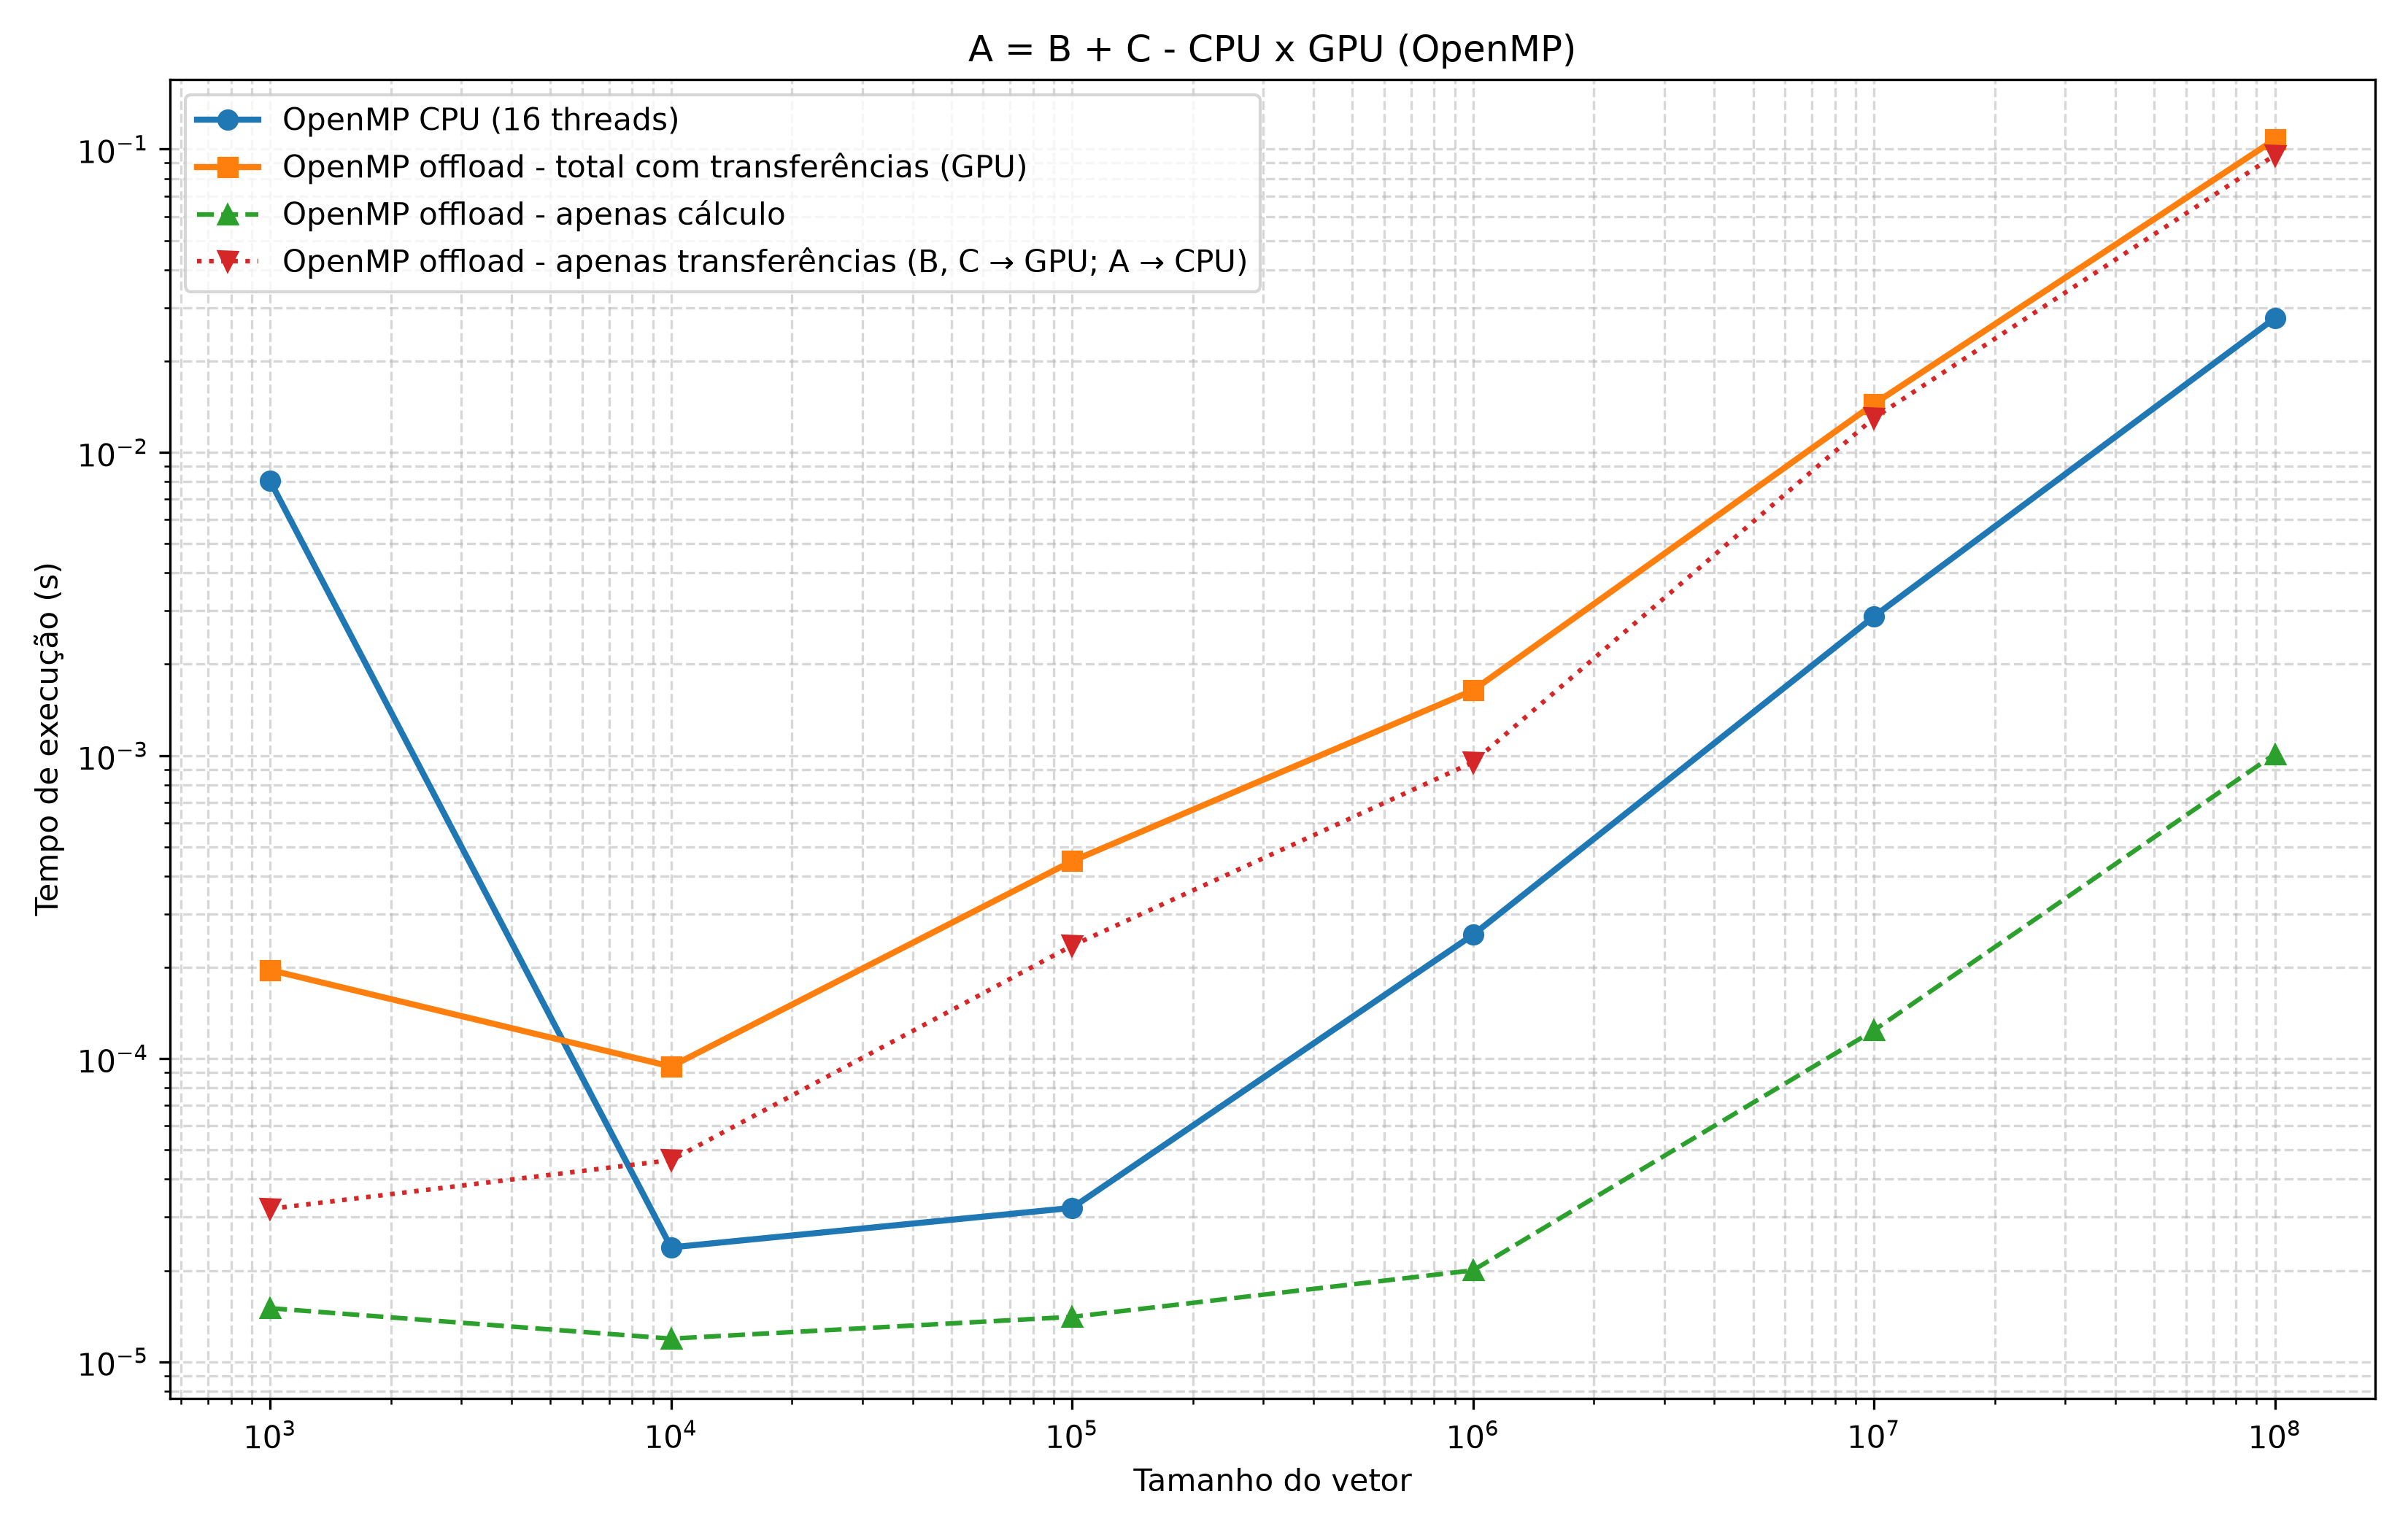
\includegraphics[width=\linewidth]{Tarefa11/tarefa11_tempos.png}
	\end{figure}
	\begin{figure}[H]
		\centering
		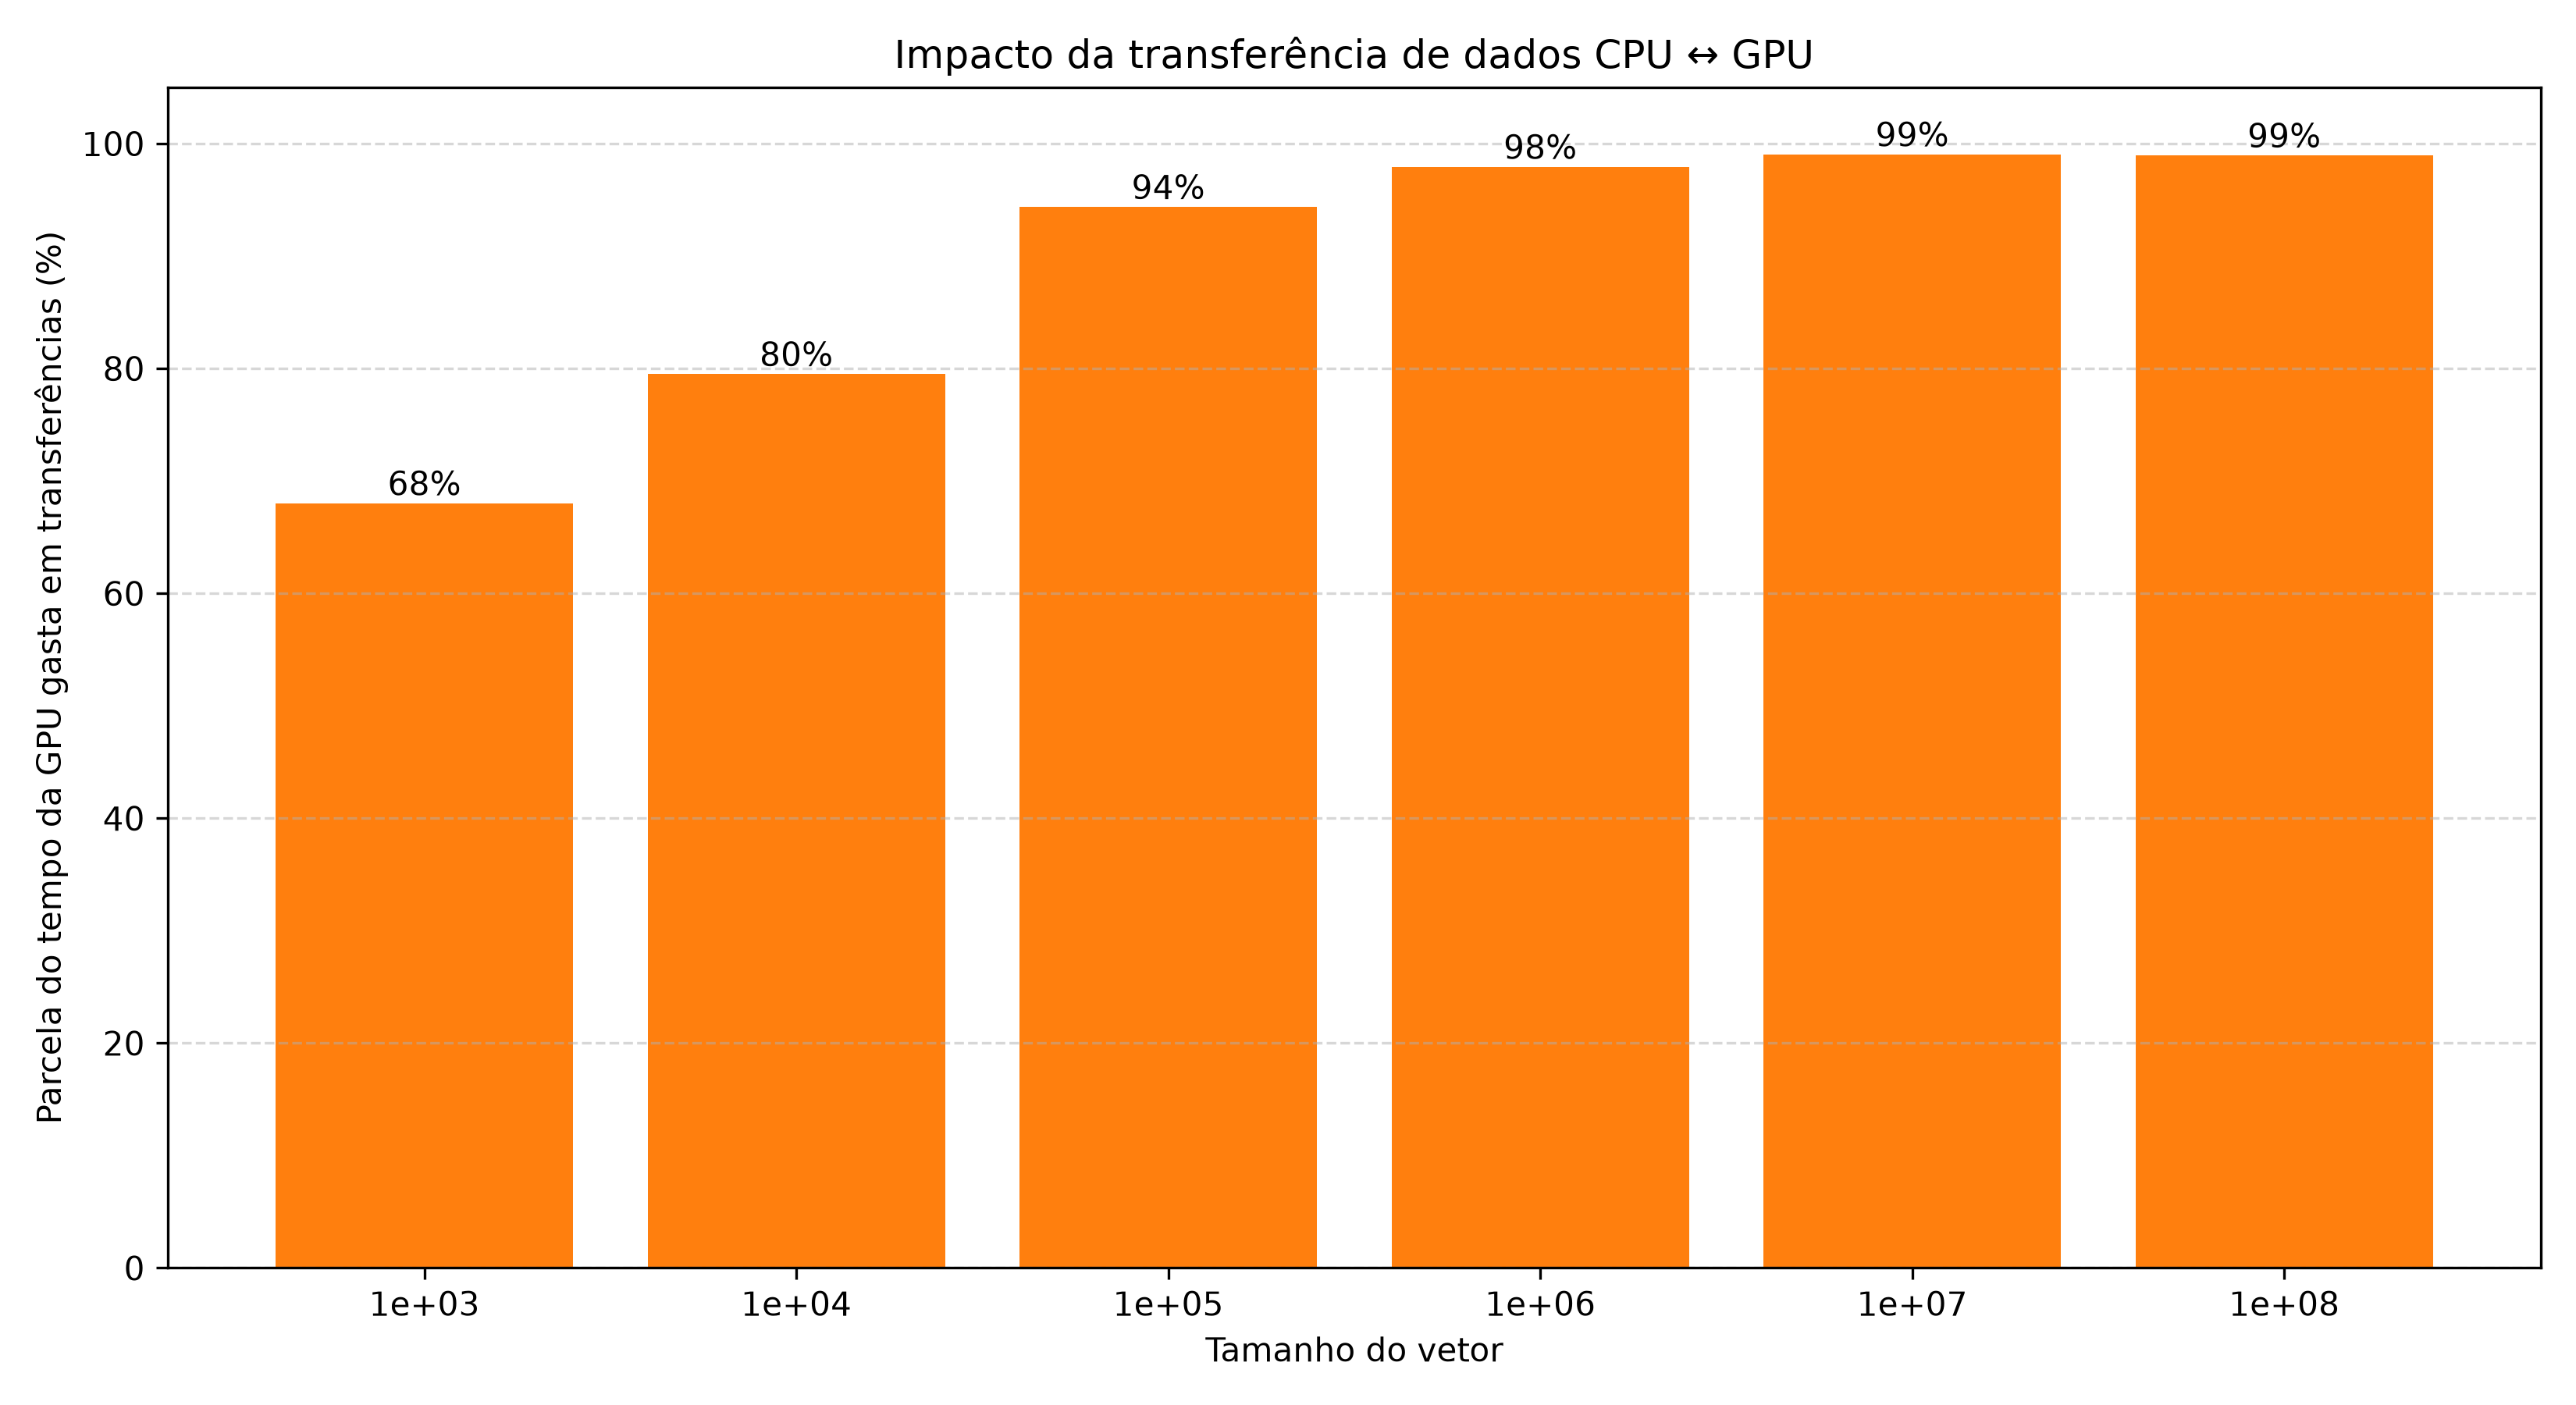
\includegraphics[width=\linewidth]{Tarefa11/tarefa11_transferencia.png}
	\end{figure}
	\par{Analisando os dados obtidos (gerados a partir da execução no supercomputador NPAD) mostrados nos gráficos, é possível verificar que o tempo de cálculo é significativamente menor durante o cálculo com GPU. Porém, ao analisarmos todo o escopo da execução, vemos que a versão paralela em CPU com OpenMP possui melhores tempos para as quantidades analisadas. Isso é causado pelo alto custo da transferência de dados entre os dispositivos, que faz com que a opção por GPU seja uma alternativa menos performática, apesar de um cálculo mais rápido.
		
		Pode-se verificar no gráfico um valor que foge do padrão apresentado durante os testes na primeira execução (o ponto mais à esquerda). Isso se deve provavelmente ao fato de ter sido justamente a primeira rodada de testes, e, portanto, os dispositivos estavam "frios". O código utilizado não considera rodadas de aquecimento, e por isso os primeiros cálculos podem apresentar certa ineficiência, como no caso verificado. }
	\subsection{\subtTres}
	\begin{lstlisting}[language=c, title=main.c]
#include <stdio.h>
#include <stdlib.h>
#include <omp.h>
#include <stddef.h>
#include <string.h>

static const size_t tamanhos[] = {
    1000,
    10000,
    100000,
    1000000,
    10000000,
    100000000
};

#define NUM_TAMANHOS (sizeof(tamanhos) / sizeof(tamanhos[0]))

typedef struct {
    float *A;
    float *B;
    float *C;
} Vetores;

Vetores* criarVetor(size_t tamanho)
{
    Vetores *v = malloc(sizeof(Vetores));

    if (v == NULL) {
        exit(EXIT_FAILURE);
    }

    v->A = malloc(tamanho * sizeof(float));
    v->B = malloc(tamanho * sizeof(float));
    v->C = malloc(tamanho * sizeof(float));

    if (v->A == NULL || v->B == NULL || v->C == NULL) {
        free(v->A);
        free(v->B);
        free(v->C);
        free(v);
        exit(EXIT_FAILURE);
    }

    #pragma omp parallel for
    for (size_t i = 0; i < tamanho; i++) {
        v->B[i] = (float)i;
        v->C[i] = (float)(i * 2);
        v->A[i] = 0.0f;
    }

    return v;
}

void liberarVetores(Vetores *v)
{
    free(v->A);
    free(v->B);
    free(v->C);
    free(v);
}

double calcularCPU(Vetores *v, size_t tamanho)
{
    double inicio = omp_get_wtime();

    #pragma omp parallel for
    for (size_t i = 0; i < tamanho; i++) {
        v->A[i] = v->B[i] + v->C[i];
    }

    return omp_get_wtime() - inicio;
}

double calcularGPU(Vetores *v, size_t tamanho)
{
    float *A = v->A;
    float *B = v->B;
    float *C = v->C;

    double inicio = omp_get_wtime();

    #pragma omp target teams distribute parallel for \
        map(to: B[0:tamanho], C[0:tamanho]) \
        map(from: A[0:tamanho])
    for (size_t i = 0; i < tamanho; i++) {
        A[i] = B[i] + C[i];
    }

    return omp_get_wtime() - inicio;
}

double calcularGPUSeparado(Vetores *v, size_t tamanho, double *transferencia)
{
    float *A = v->A;
    float *B = v->B;
    float *C = v->C;

    double inicio = omp_get_wtime();

    #pragma omp target enter data map(to: B[0:tamanho], C[0:tamanho]) \
        map(alloc: A[0:tamanho])

    double inicioKernel = omp_get_wtime();

    #pragma omp target teams distribute parallel for
    for (size_t i = 0; i < tamanho; i++) {
        A[i] = B[i] + C[i];
    }

    double tempoKernel = omp_get_wtime() - inicioKernel;

    #pragma omp target exit data map(from: A[0:tamanho]) \
        map(release: B[0:tamanho], C[0:tamanho])

    *transferencia = (omp_get_wtime() - inicio) - tempoKernel;

    return tempoKernel;
}

int verificarResultado(Vetores *v, size_t tamanho)
{
    for (size_t i = 0; i < tamanho; i++) {
        if (v->A[i] != v->B[i] + v->C[i]) {
            return 0;
        }
    }

    return 1;
}

int main(void)
{
    FILE *arquivo = fopen("resultados.json", "w");

    if (arquivo == NULL) {
        return EXIT_FAILURE;
    }

    #pragma omp target
    {
    }

    fprintf(arquivo, "{\n  \"dispositivos\": %d,\n  \"threads\": %d,\n  \"resultados\": [\n",
            omp_get_num_devices(), omp_get_max_threads());

    for (size_t i = 0; i < NUM_TAMANHOS; i++) {
        size_t tamanho = tamanhos[i];

        Vetores *v = criarVetor(tamanho);

        double tempoCPU = calcularCPU(v, tamanho);

        if (!verificarResultado(v, tamanho)) {
            liberarVetores(v);
            fclose(arquivo);
            return EXIT_FAILURE;
        }

        memset(v->A, 0, tamanho * sizeof(float));

        double tempoGPU = calcularGPU(v, tamanho);

        if (!verificarResultado(v, tamanho)) {
            liberarVetores(v);
            fclose(arquivo);
            return EXIT_FAILURE;
        }

        memset(v->A, 0, tamanho * sizeof(float));

        double tempoTransferencia = 0.0;
        double tempoKernel = calcularGPUSeparado(v, tamanho, &tempoTransferencia);

        if (!verificarResultado(v, tamanho)) {
            liberarVetores(v);
            fclose(arquivo);
            return EXIT_FAILURE;
        }

        fprintf(arquivo,
                "    {\"tamanho\": %zu, \"cpu_s\": %.10f, \"gpu_total_s\": %.10f, "
                "\"gpu_kernel_s\": %.10f, \"gpu_transferencia_s\": %.10f}%s\n",
                tamanho, tempoCPU, tempoGPU, tempoKernel, tempoTransferencia,
                i + 1 < NUM_TAMANHOS ? "," : "");

        printf("%zu: CPU = %.10f s | GPU = %.10f s (kernel %.10f s + transferencia %.10f s)\n",
               tamanho, tempoCPU, tempoGPU, tempoKernel, tempoTransferencia);

        liberarVetores(v);
    }

    fprintf(arquivo, "  ]\n}\n");
    fclose(arquivo);

    return EXIT_SUCCESS;
}
\end{lstlisting}
	\begin{lstlisting}[language=bash, title=script\_gpu.sh]
#!/bin/bash
#SBATCH --job-name=OMP_GPU_vetor_akira
#SBATCH --output=saida%j.out
#SBATCH --error=erro%j.err
#SBATCH --partition=gpu-4-a100
#SBATCH --nodes=1
#SBATCH --ntasks=1
#SBATCH --cpus-per-task=16
#SBATCH --gpus-per-node=1
#SBATCH --time=0-0:10

cd "${SLURM_SUBMIT_DIR:-.}"
mkdir -p outputs
export OMP_NUM_THREADS=${SLURM_CPUS_PER_TASK:-16}

nvidia-smi --query-gpu=name,memory.total --format=csv 2> /dev/null

carrega_nvhpc() {
    command -v nvc > /dev/null 2>&1 && return 0
    if ! type module > /dev/null 2>&1; then
        for f in /etc/profile.d/modules.sh /etc/profile.d/lmod.sh /usr/share/lmod/lmod/init/bash; do
            [ -f "$f" ] && source "$f" && break
        done
    fi
    type module > /dev/null 2>&1 || return 1
    local mod=${NVHPC_MODULE:-$(module -t avail 2>&1 | grep -v ':$' | grep -vE '^(containers|softwares)/' | grep -i 'nvhpc' | sort -V | tail -n 1)}
    [ -n "$mod" ] && echo "Carregando modulo: $mod" && module load "$mod"
    command -v nvc > /dev/null 2>&1
}

if carrega_nvhpc && nvc -O2 -mp=gpu main.c -o outputs/main 2> outputs/build_nvc.log; then
    echo "Compilado com NVHPC (-mp=gpu)"
elif gcc -O2 -fopenmp -foffload=nvptx-none -fno-stack-protector main.c -o outputs/main 2> outputs/build_gcc.log; then
    echo "Compilado com GCC + nvptx-none"
else
    echo "Sem compilador com offload (veja outputs/build_*.log)" >&2
    exit 1
fi

./outputs/main

if command -v python3 > /dev/null 2>&1 && python3 -c "import matplotlib" 2> /dev/null; then
    python3 plot.py
fi
\end{lstlisting}
	
	\newpage
	\onehalfspacing
	\section{TAREFA 12}
	\subsection{\subtUm}
	\par{Paralelizar o código de propagação de onda com OpenMP, com foco na execução em threads da CPU, e executar os experimentos em um único nó do NPAD, variando o número de threads de 1 a 32.
		
		Analisar a escalabilidade forte, mantendo o tamanho do problema fixo, e a escalabilidade fraca, aumentando o problema proporcionalmente ao número de threads, apresentando gráficos de speedup e eficiência.
		
		Avaliar como o desempenho e a escalabilidade são afetados pelas diferentes políticas de afinidade de threads do sistema operacional e do OpenMP.}
	\subsection{\subtDois}
	\begin{figure}[H]
		\centering
		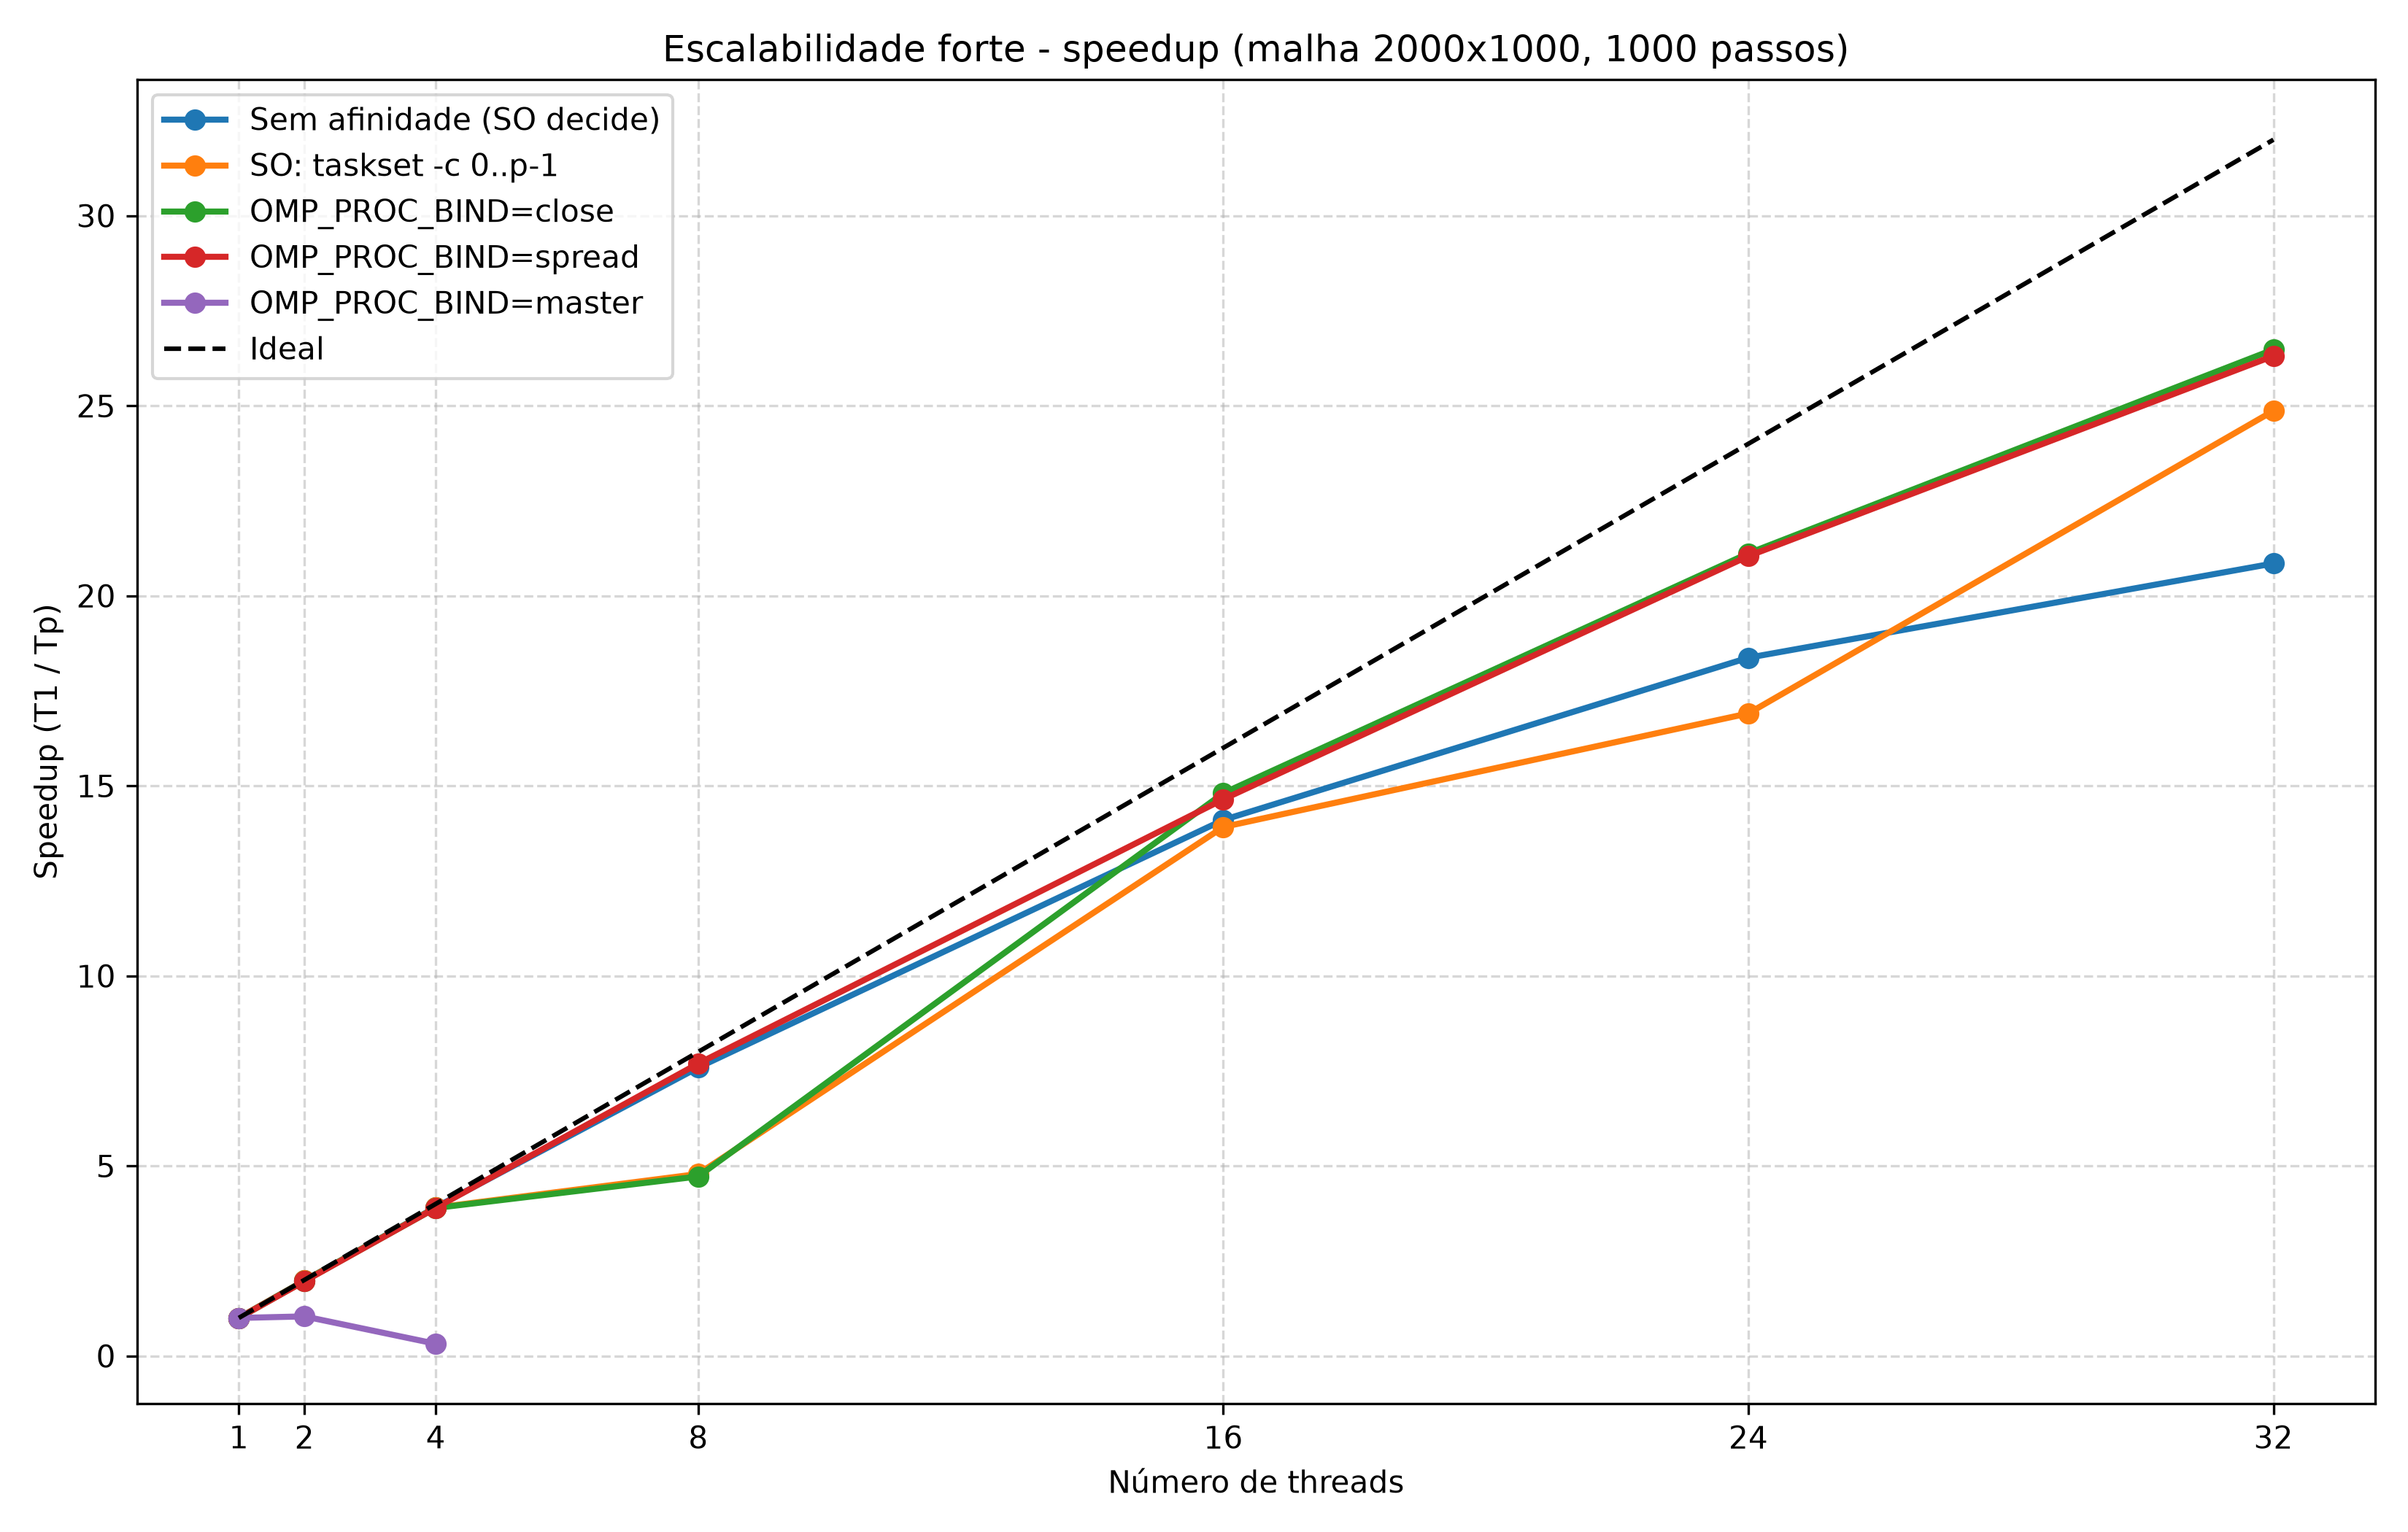
\includegraphics[width=\linewidth]{Tarefa12/tarefa12_speedup.png}
	\end{figure}
	\begin{figure}[H]
		\centering
		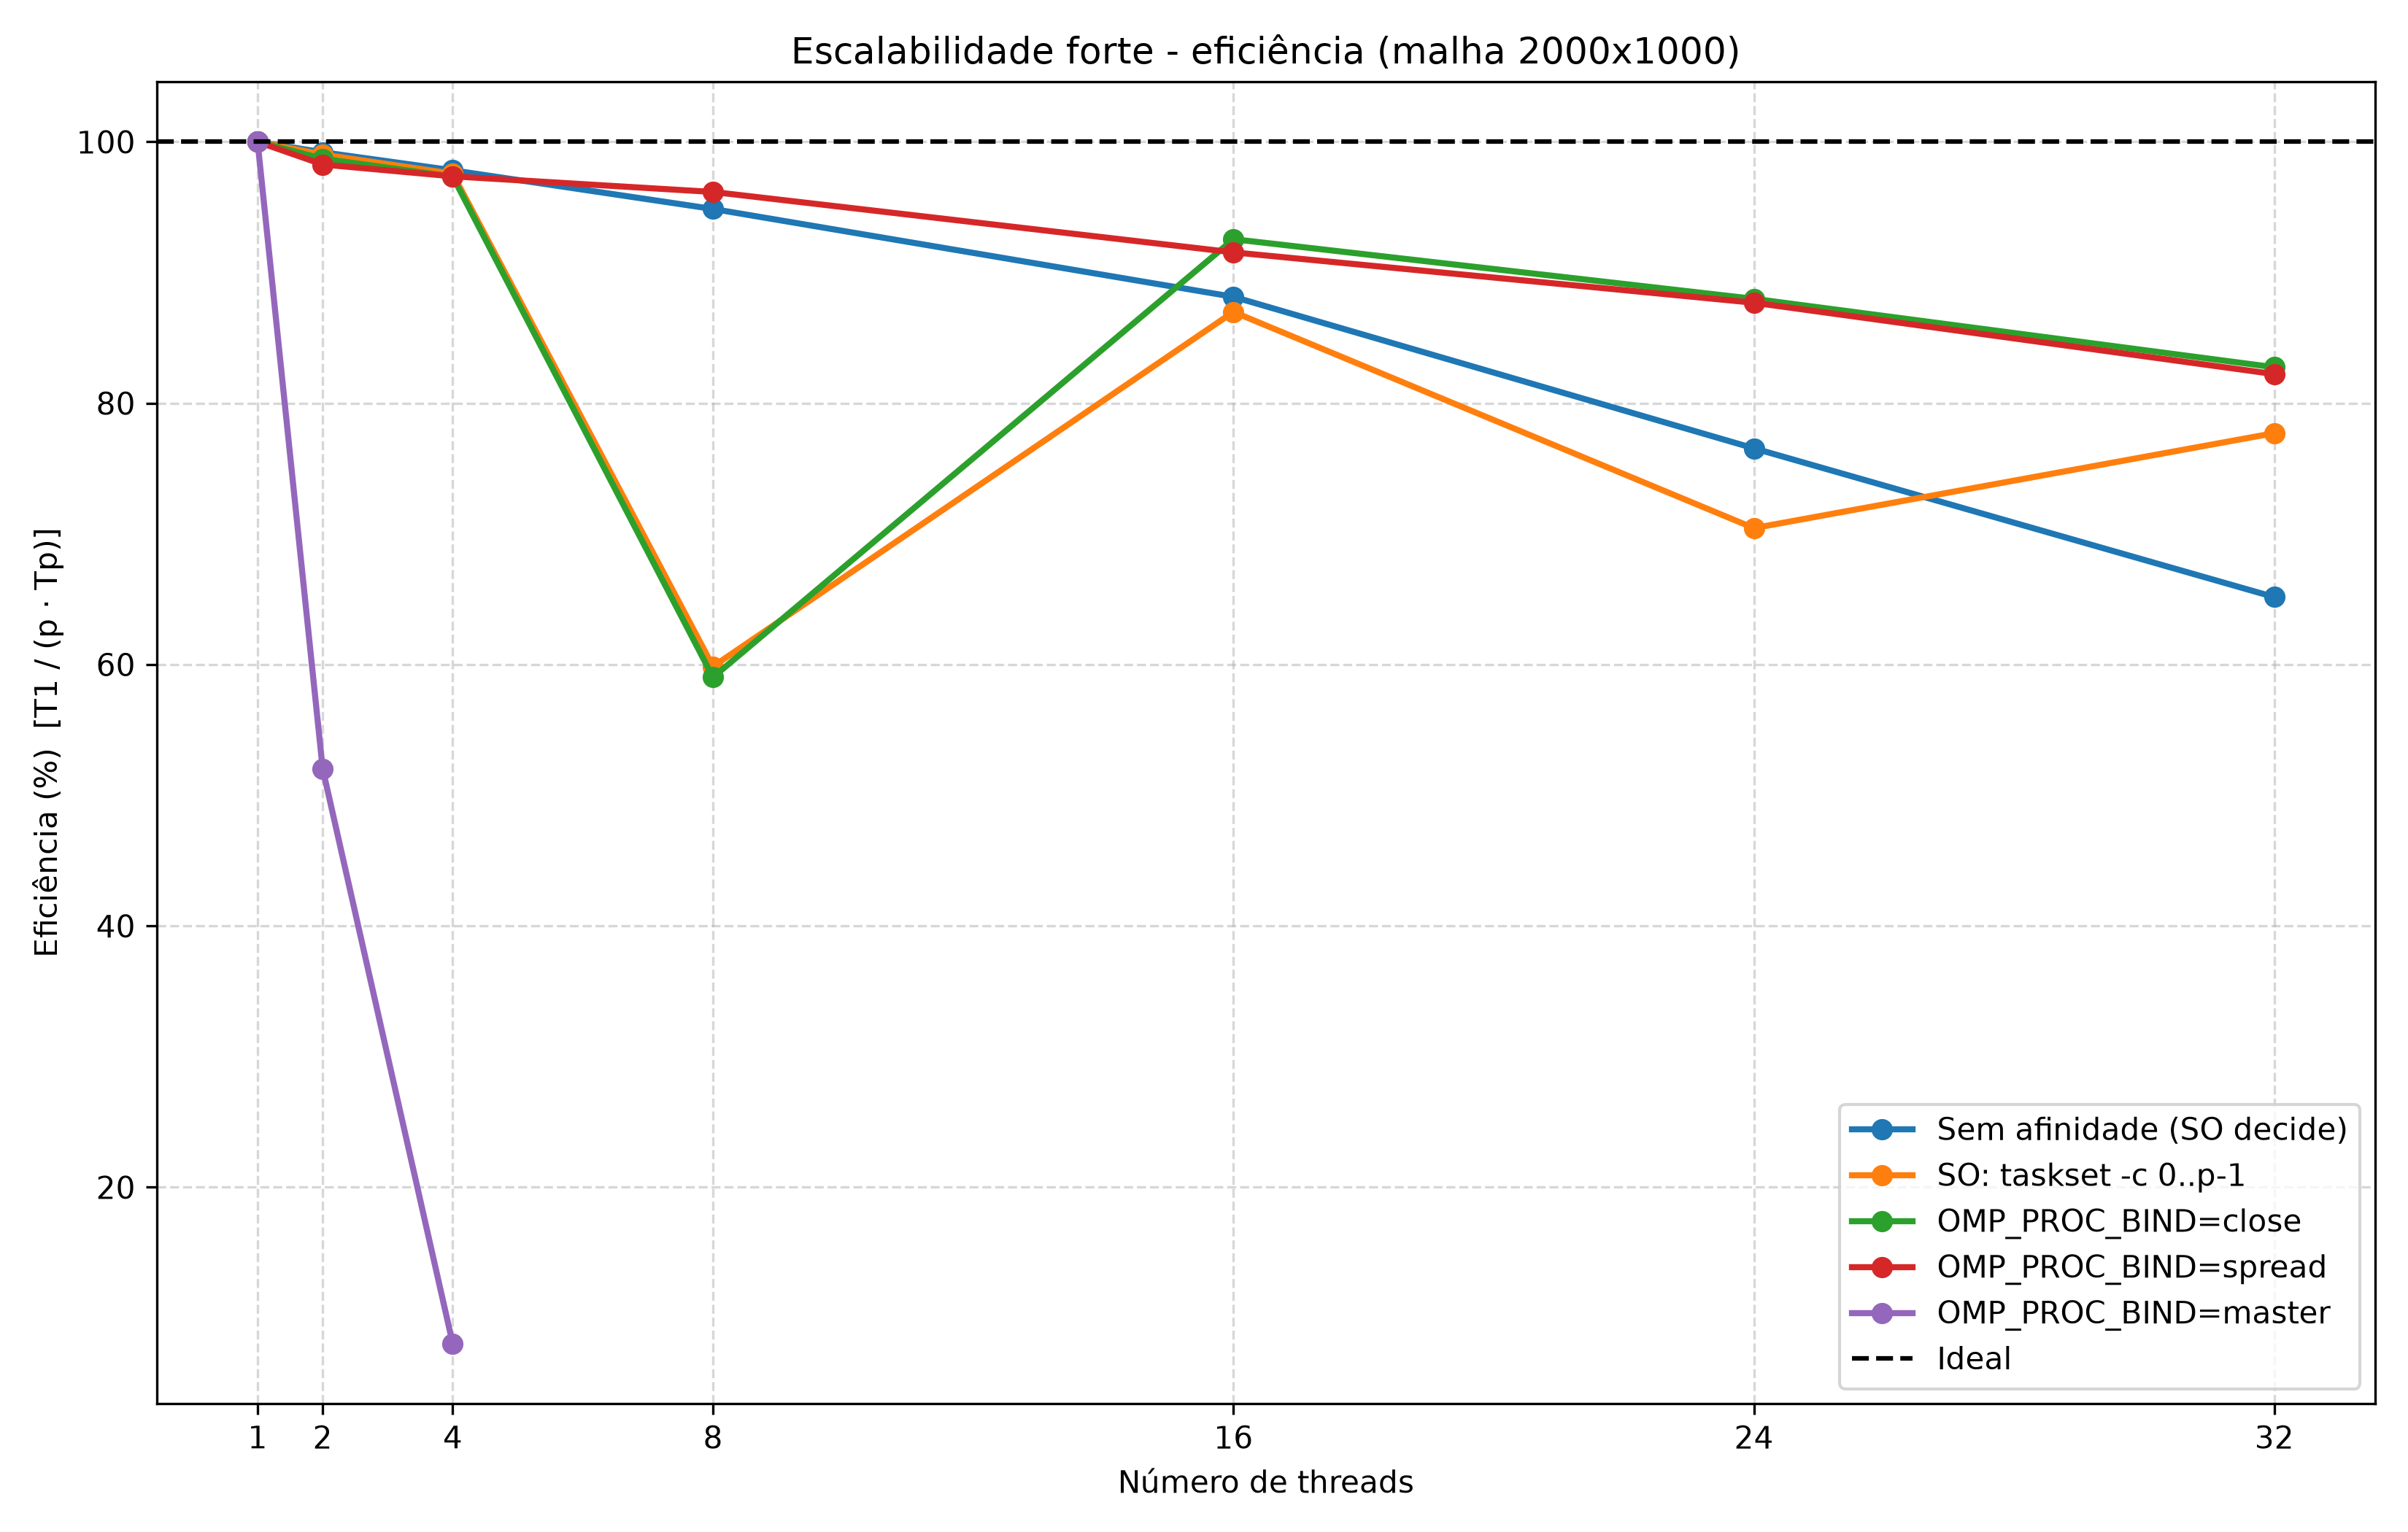
\includegraphics[width=\linewidth]{Tarefa12/tarefa12_eficiencia.png}
	\end{figure}
	\begin{figure}
		\centering
		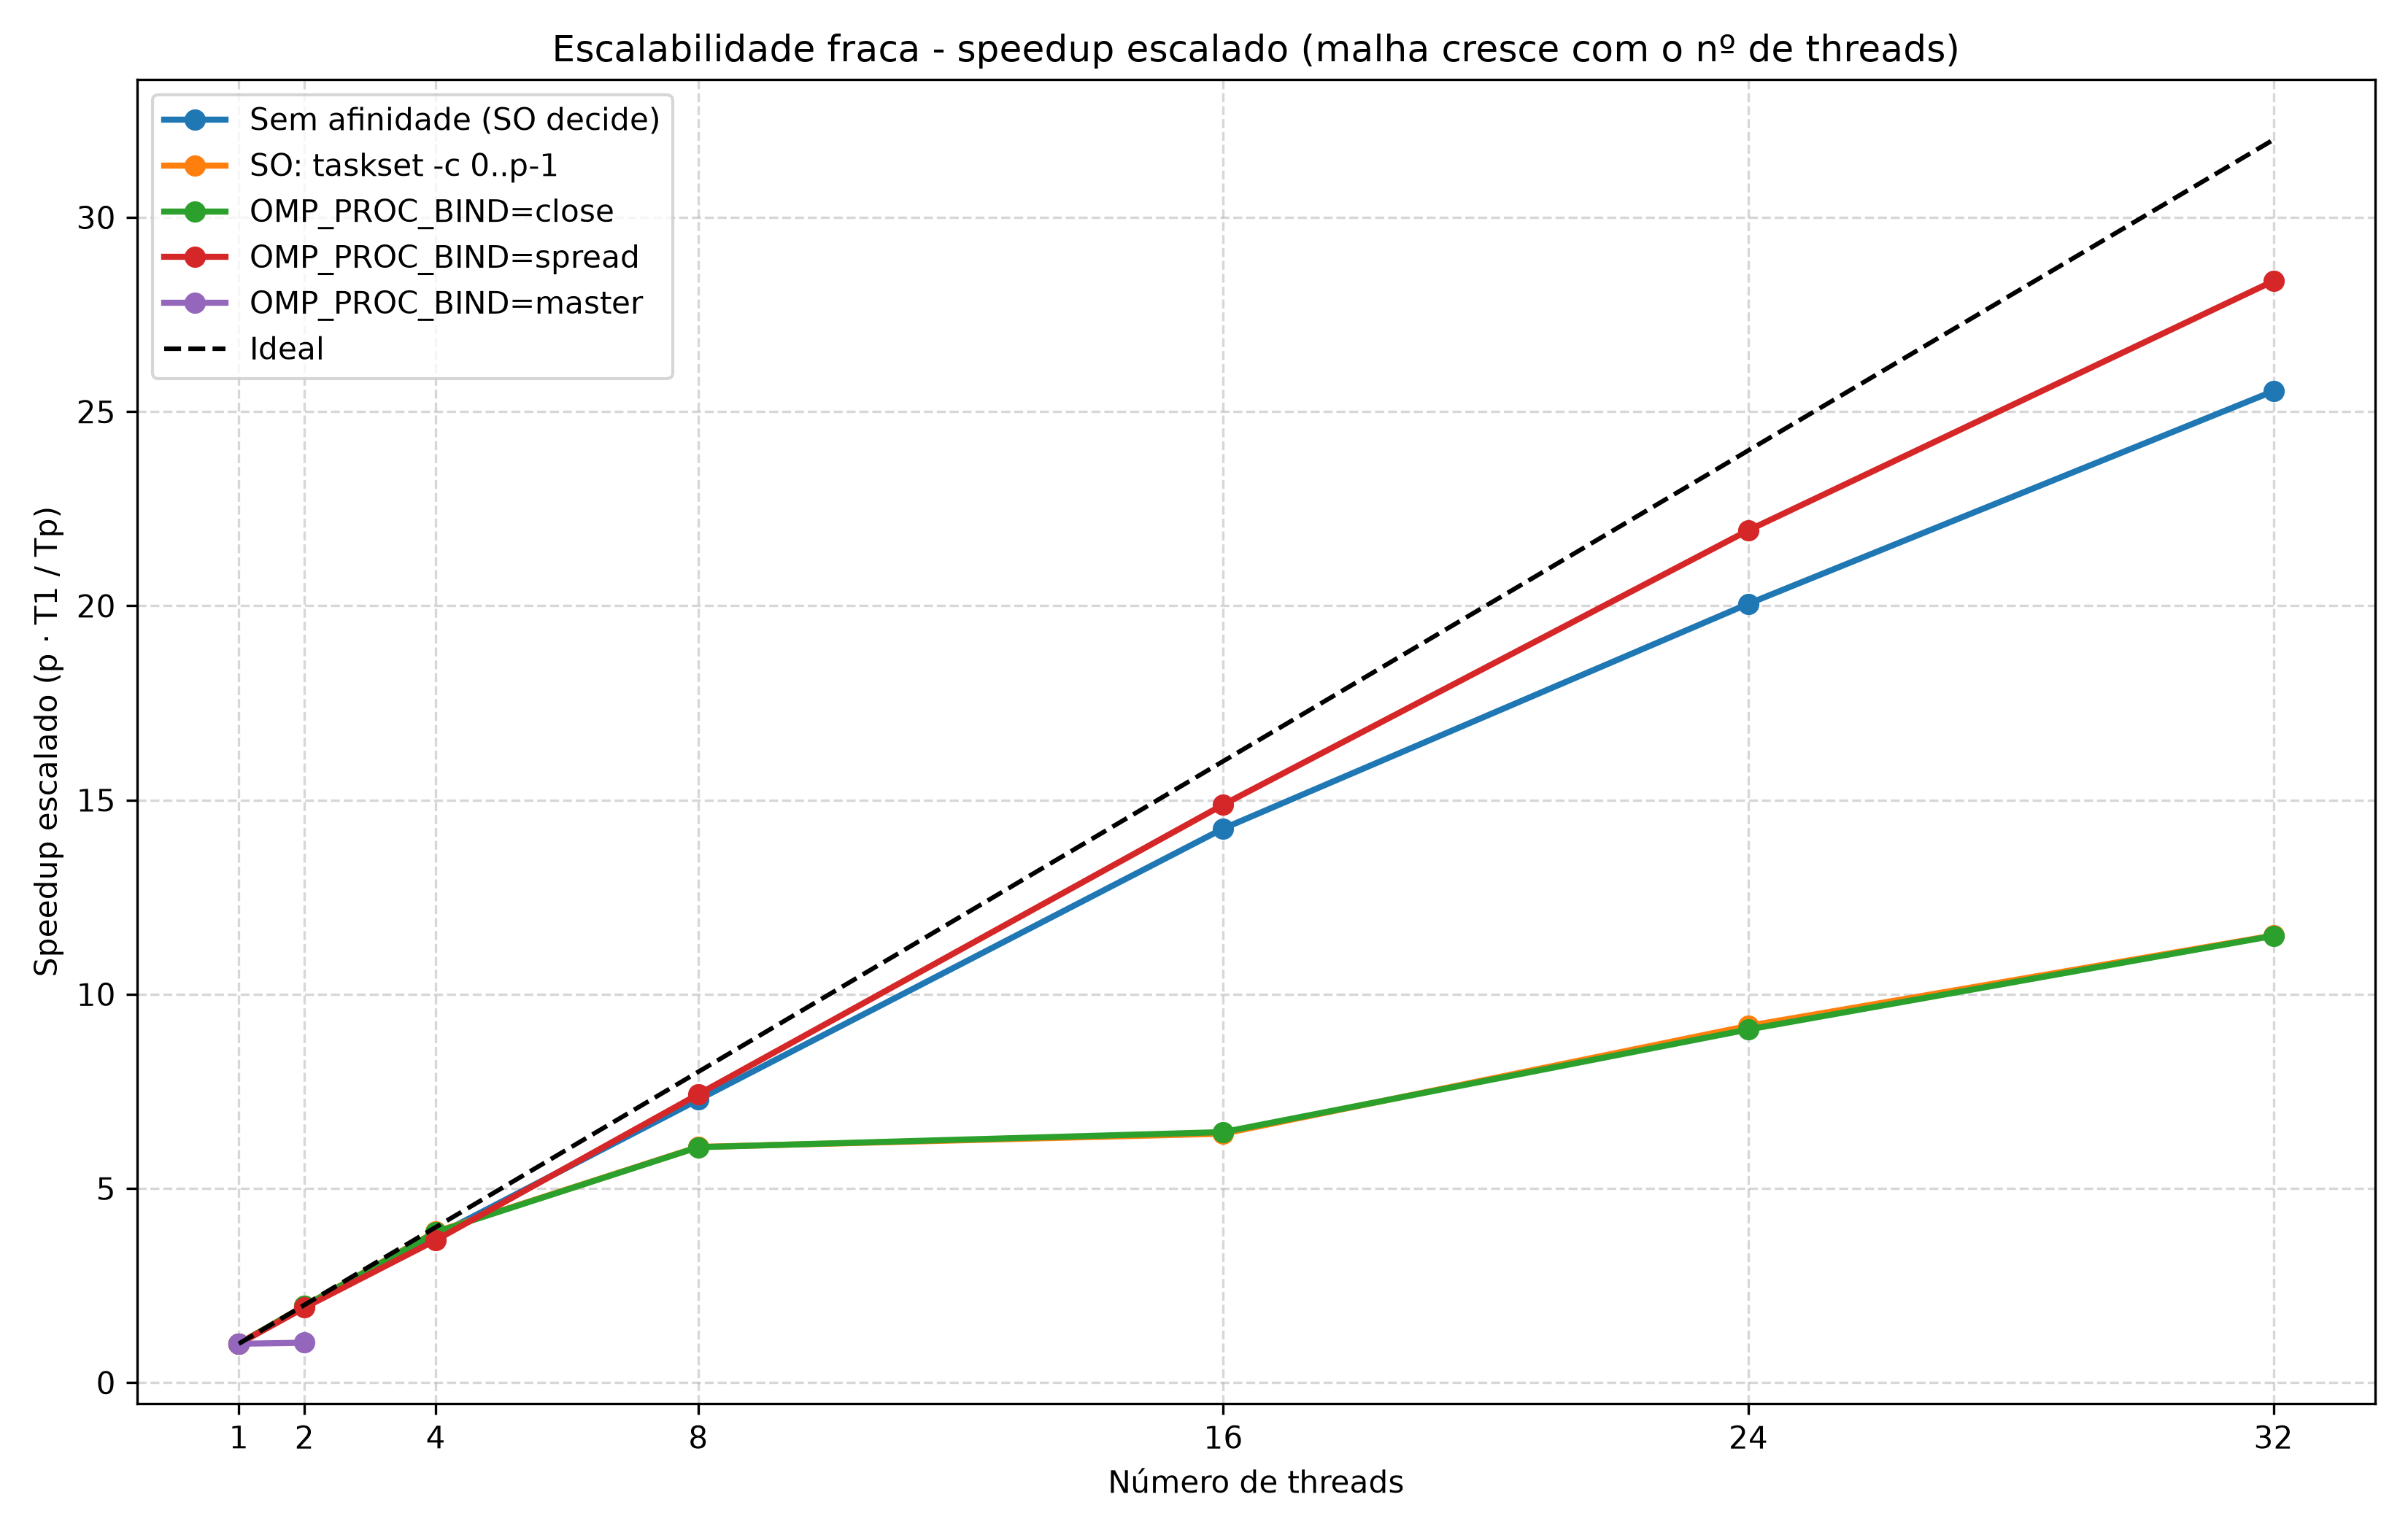
\includegraphics[width=\linewidth]{Tarefa12/tarefa12_speedup_fraca.png}
	\end{figure}
	\begin{figure}[H]
		\centering
		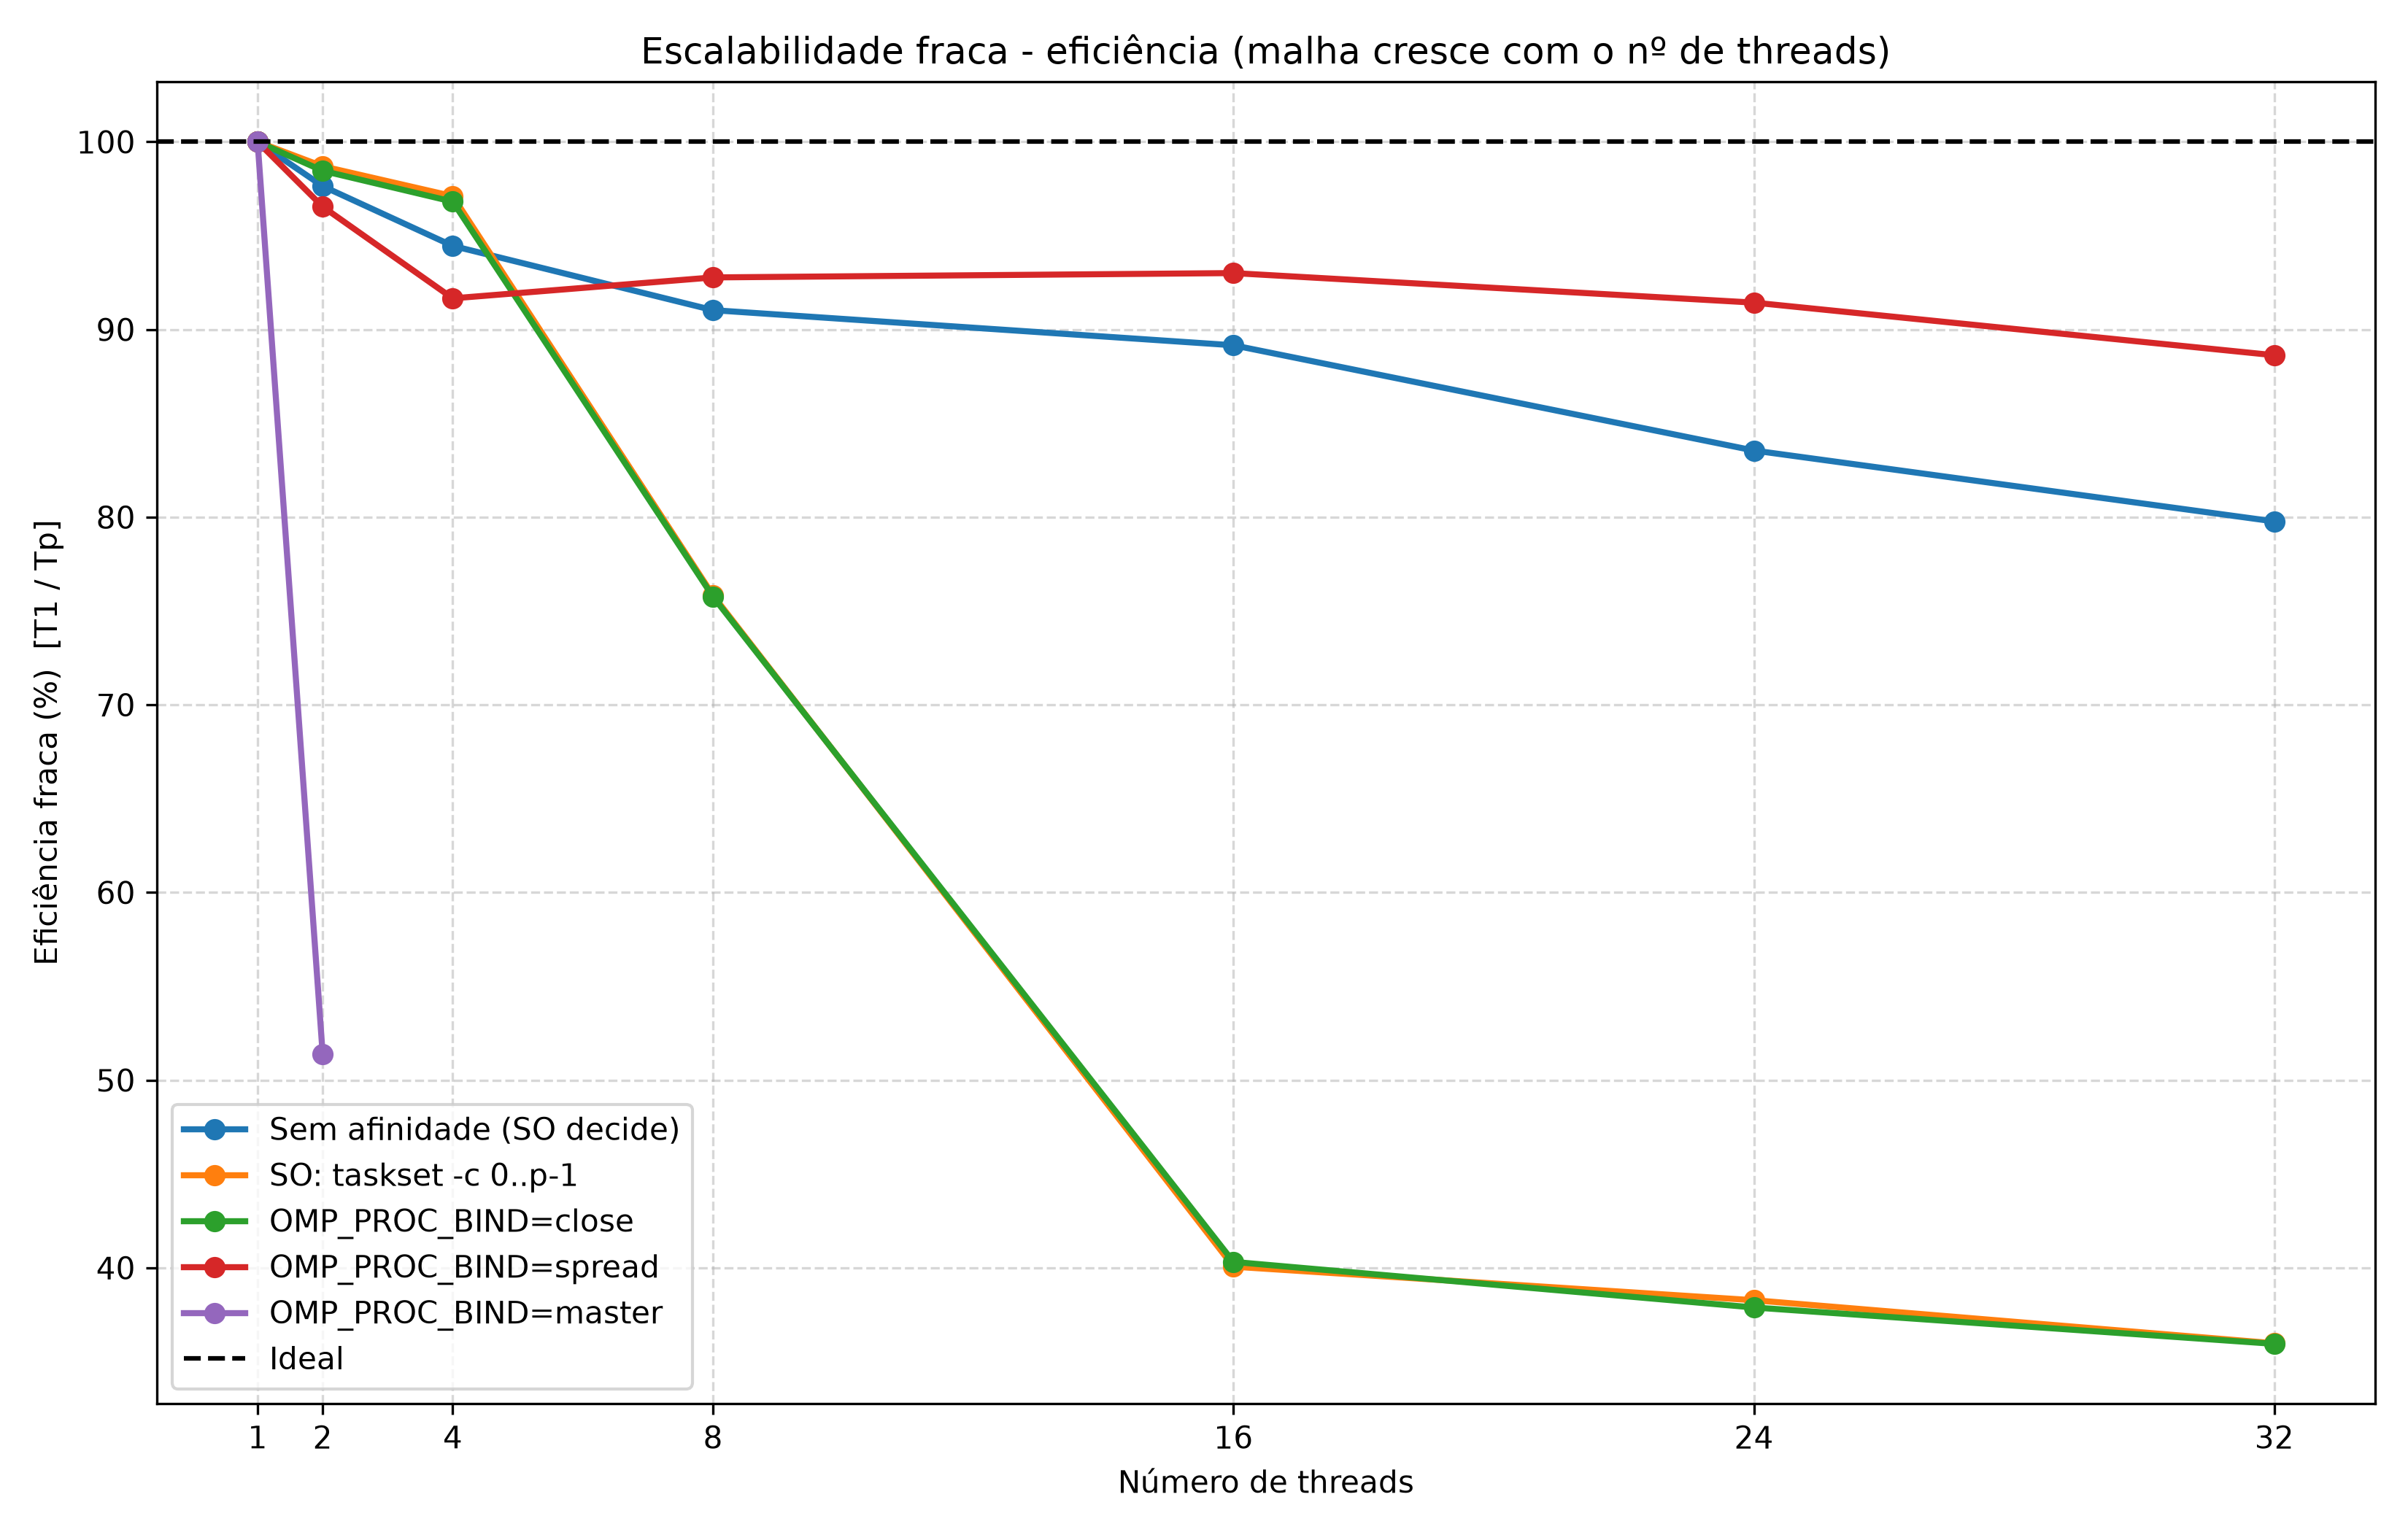
\includegraphics[width=\linewidth]{Tarefa12/tarefa12_fraca.png}
	\end{figure}
	\begin{figure}[H]
		\centering
		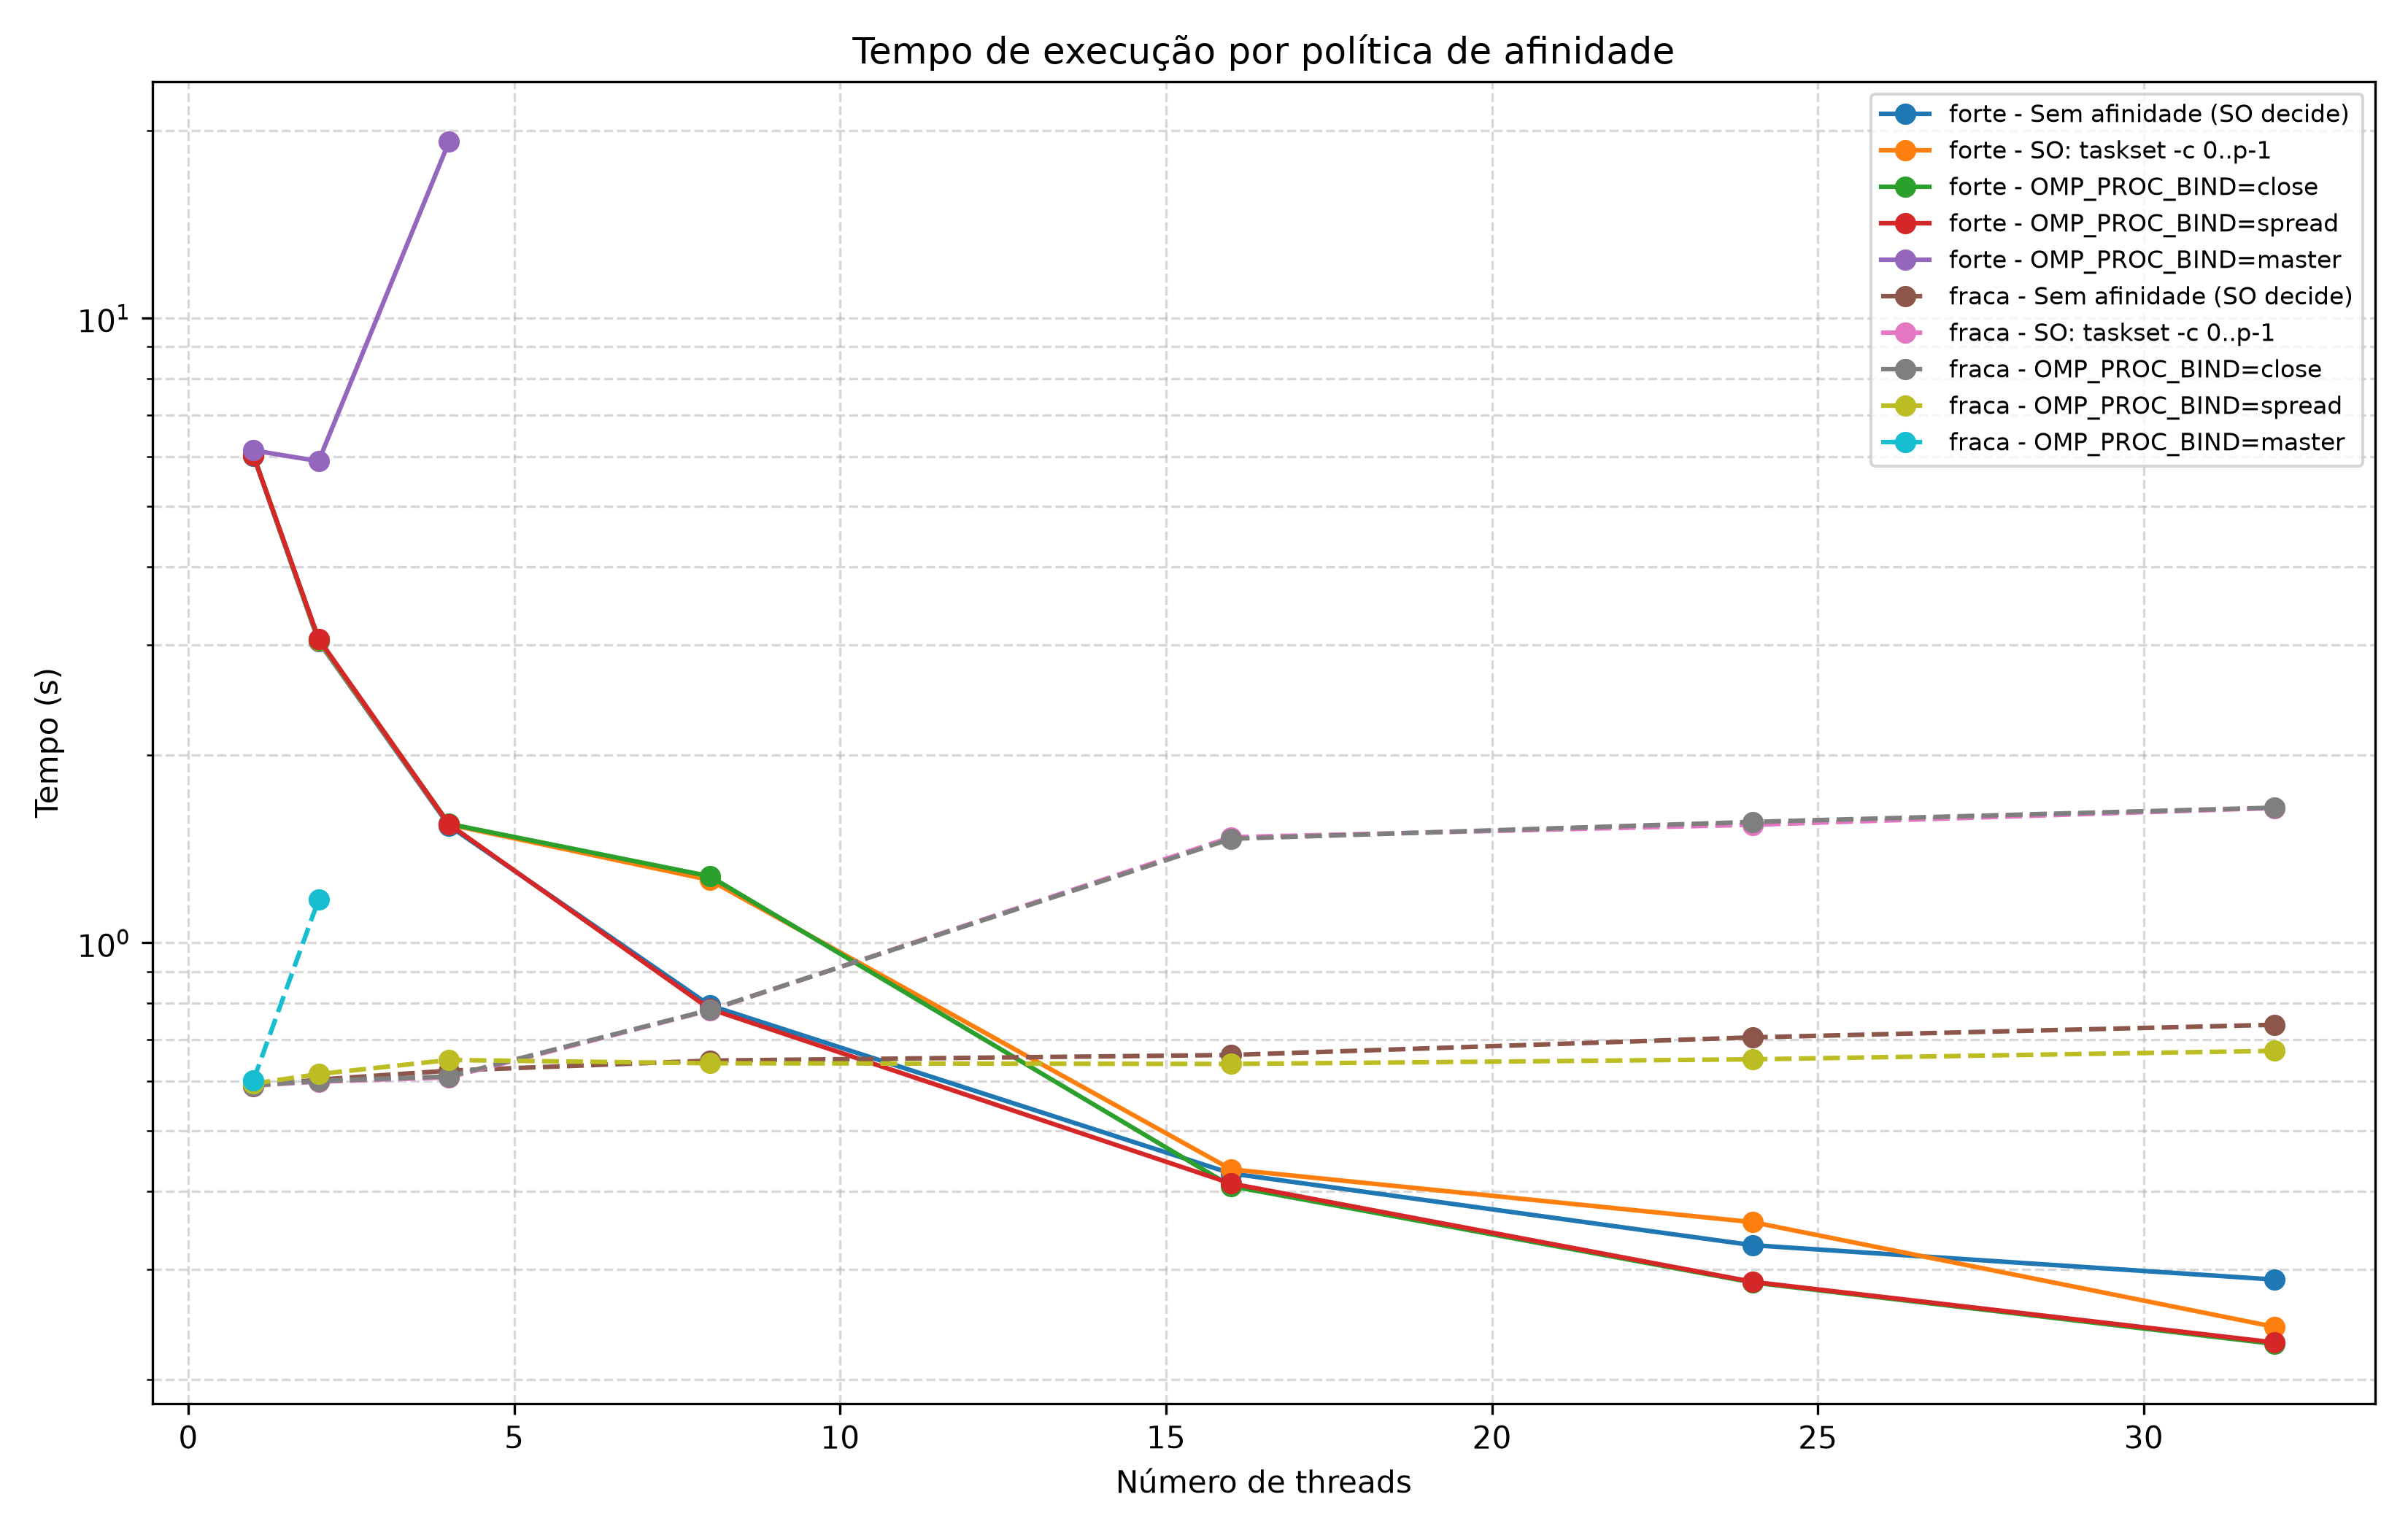
\includegraphics[width=\linewidth]{Tarefa12/tarefa12_tempos.png}
	\end{figure}
	\par{
		Analisando os dados e gráficos gerados, podemos notar alguns pontos importantes. 
		
		O primeiro é que a política master teve performance consideravelmente pior do que as outras, chegando a um fator de speedup nulo. Além disso, seus fatores de escalabilidade e tempo de execução mostram que, para esse tipo de problema, não é uma opção viável.
		
		A opção sem escolha de afinidade se mostra mais próxima aos outros resultados, mas ainda inferior às outras opções, exceto quando se tratando de escalabilidade fraca, em que  perde somente para a afinidade spread. O contrário ocorre com a política close, que se mostra em par com a spread para os casos de escalabilidade forte, mas perde performance para escalabilidade fraca.
		
		Portanto, a melhor escolha para esse tipo de algorítmo é a política de afinidade spread, que apresenta os melhores números de desempenho em todos os casos analisados quando comparado às suas alternativas.
	}
	\subsection{\subtTres}
	\begin{lstlisting}[language=c, title=main.c]
#include <stdio.h>
#include <stdlib.h>
#include <math.h>
#include <omp.h>

static int NX = 200;
static int NZ = 100;

#define DX 10.0
#define DZ 10.0

#define DT 0.001
#define NT 1000

#define VELOCIDADE 2000.0

#define SX 100
#define SZ 50

#define RX 150
#define RZ 50

#define PI 3.14159265358979323846

double ricker(double t, double f0)
{
    double t0 = 1.0 / f0;

    double x = PI * f0 * (t - t0);

    return (1.0 - 2.0 * x * x) * exp(-x * x);
}

void inicializa_modelo(double *vel)
{
    for (int iz = 0; iz < NZ; iz++)
    {
        for (int ix = 0; ix < NX; ix++)
        {

            vel[iz * NX + ix] = VELOCIDADE;
        }
    }
}

void salva_binario(
    const char *nome,
    double *campo)
{
    FILE *fp = fopen(nome, "wb");

    if (fp == NULL)
    {
        perror("Erro ao abrir arquivo");
        exit(EXIT_FAILURE);
    }

    fwrite(
        campo,
        sizeof(double),
        NX * NZ,
        fp);

    fclose(fp);
}

int main(int argc, char *argv[])
{
    int salvar = 1;
    const char *rotulo = "padrao";

    if (argc > 2)
    {
        NX = atoi(argv[1]);
        NZ = atoi(argv[2]);
    }
    if (argc > 3)
        salvar = atoi(argv[3]);
    if (argc > 4)
        rotulo = argv[4];

    double *vel = malloc(NX * NZ * sizeof(double));

    double *u = calloc(NX * NZ, sizeof(double));

    double *u_old = calloc(NX * NZ, sizeof(double));

    double *u_new = calloc(NX * NZ, sizeof(double));

    if (!vel || !u || !u_old || !u_new)
    {
        printf("Erro de alocacao de memoria\n");
        return 1;
    }

    inicializa_modelo(vel);

    FILE *receiver = fopen("receiver.dat", "w");

    if (receiver == NULL)
    {
        printf("Erro ao abrir receiver.dat\n");
        return 1;
    }

    double f0 = 20.0;

    double dt2 = DT * DT;

    double inicio = omp_get_wtime();

    for (int it = 0; it < NT; it++)
    {

        double t = it * DT;

#pragma omp parallel for collapse(2)
        for (int iz = 1; iz < NZ - 1; iz++)
        {

            for (int ix = 1; ix < NX - 1; ix++)
            {

                int id = iz * NX + ix;

                double d2udx2 =
                    (u[id + 1] - 2.0 * u[id] + u[id - 1]) / (DX * DX);

                double d2udz2 =
                    (u[id + NX] - 2.0 * u[id] + u[id - NX]) / (DZ * DZ);

                u_new[id] =
                    2.0 * u[id] - u_old[id] + vel[id] * vel[id] * dt2 * (d2udx2 + d2udz2);
            }
        }

        int source_id = SZ * NX + SX;

        u_new[source_id] += ricker(t, f0);

        int receiver_id = RZ * NX + RX;

        fprintf(
            receiver,
            "%lf %lf\n",
            t,
            u_new[receiver_id]);

        char nome[100];

        sprintf(
            nome,
            "wavefield_%04d.bin",
            it);

        if (salvar)
            salva_binario(nome, u_new);

        double *tmp;

        tmp = u_old;
        u_old = u;

        u = u_new;

        u_new = tmp;

        if (it % 100 == 0)
        {
            printf(
                "Passo %d / %d\n",
                it,
                NT);
        }
    }

    double tempo = omp_get_wtime() - inicio;

    fclose(receiver);

    const char *bind = getenv("OMP_PROC_BIND");
    const char *places = getenv("OMP_PLACES");

    FILE *saida = fopen("resultados.out", "a");
    if (saida != NULL)
    {
        fprintf(saida,
                "{\"experimento\": \"%s\", \"nx\": %d, \"nz\": %d, \"nt\": %d, "
                "\"threads\": %d, \"proc_bind\": \"%s\", \"places\": \"%s\", "
                "\"tempo_s\": %.6f}\n",
                rotulo, NX, NZ, NT, omp_get_max_threads(),
                bind ? bind : "padrao", places ? places : "padrao", tempo);
        fclose(saida);
    }

    printf("Tempo: %.6f s (%d threads, %dx%d)\n", tempo, omp_get_max_threads(), NX, NZ);

    free(vel);
    free(u);
    free(u_old);
    free(u_new);

    printf("\nSimulacao finalizada.\n");

    return 0;
}
\end{lstlisting}
	\begin{lstlisting}[language=bash, title=script\_job.sh]
#!/bin/bash
#SBATCH --job-name=OMP_onda_akira
#SBATCH --output=saida%j.out
#SBATCH --error=erro%j.err
#SBATCH --partition=amd-512
#SBATCH --nodes=1
#SBATCH --ntasks=1
#SBATCH --cpus-per-task=32
#SBATCH --exclusive
#SBATCH --hint=compute_bound
#SBATCH --time=0-0:40

cd "${SLURM_SUBMIT_DIR:-.}"
mkdir -p outputs

gcc -O2 -fopenmp main.c -o outputs/main -lm || exit 1

THREADS="1 2 4 8 16 24 32" bash experimentos.sh

if command -v python3 > /dev/null 2>&1 && python3 -c "import matplotlib" 2> /dev/null; then
    python3 plot.py
fi
\end{lstlisting}
	\begin{lstlisting}[language=bash, title=experimentos.sh]
#!/bin/bash
cd "$(dirname "$0")"

THREADS="${THREADS:-1 2 4 8 16 24 32}"
AFINIDADES="${AFINIDADES:-false taskset close spread master}"
THREADS_MASTER="${THREADS_MASTER:-1 2 4 8 16 24 32}"
NX_FORTE=${NX_FORTE:-2000}
NZ_FORTE=${NZ_FORTE:-1000}
NX_FRACA=${NX_FRACA:-2000}
NZ_POR_THREAD=${NZ_POR_THREAD:-100}
BIN=./outputs/main

rm -f resultados.out

executa() {
    local af=$1 t=$2 nx=$3 nz=$4 exp=$5
    if [ "$af" = "taskset" ]; then
        OMP_NUM_THREADS=$t OMP_PROC_BIND=false taskset -c 0-$((t - 1)) \
            $BIN $nx $nz 0 "$exp:$af" > /dev/null
    else
        OMP_NUM_THREADS=$t OMP_PROC_BIND=$af OMP_PLACES=cores \
            $BIN $nx $nz 0 "$exp:$af" > /dev/null
    fi
    tail -n 1 resultados.out
}

for af in $AFINIDADES; do
    lista=$THREADS
    [ "$af" = "master" ] && lista=$THREADS_MASTER
    for t in $lista; do
        executa $af $t $NX_FORTE $NZ_FORTE forte
        executa $af $t $NX_FRACA $((NZ_POR_THREAD * t)) fraca
    done
done
\end{lstlisting}
	
	\newpage
	\onehalfspacing
	\section{TAREFA 13}
	\subsection{\subtUm}
	\par{Implementar duas versões paralelas do código de propagação de onda para GPU utilizando OpenMP Offloading: uma não otimizada, usando a cláusula map para as transferências, e outra otimizada, usando target data e decidindo se o offloading será feito de acordo com o tamanho do problema.
		
		Realizar experimentos com diferentes tamanhos de problema, comparando o tempo de execução e de transferência, o impacto do tamanho do problema, o overhead do offloading, os benefícios do target data e as situações em que o uso da GPU é vantajoso ou não.}
	\subsection{\subtDois}
	
	\begin{figure}[H]
		\centering
		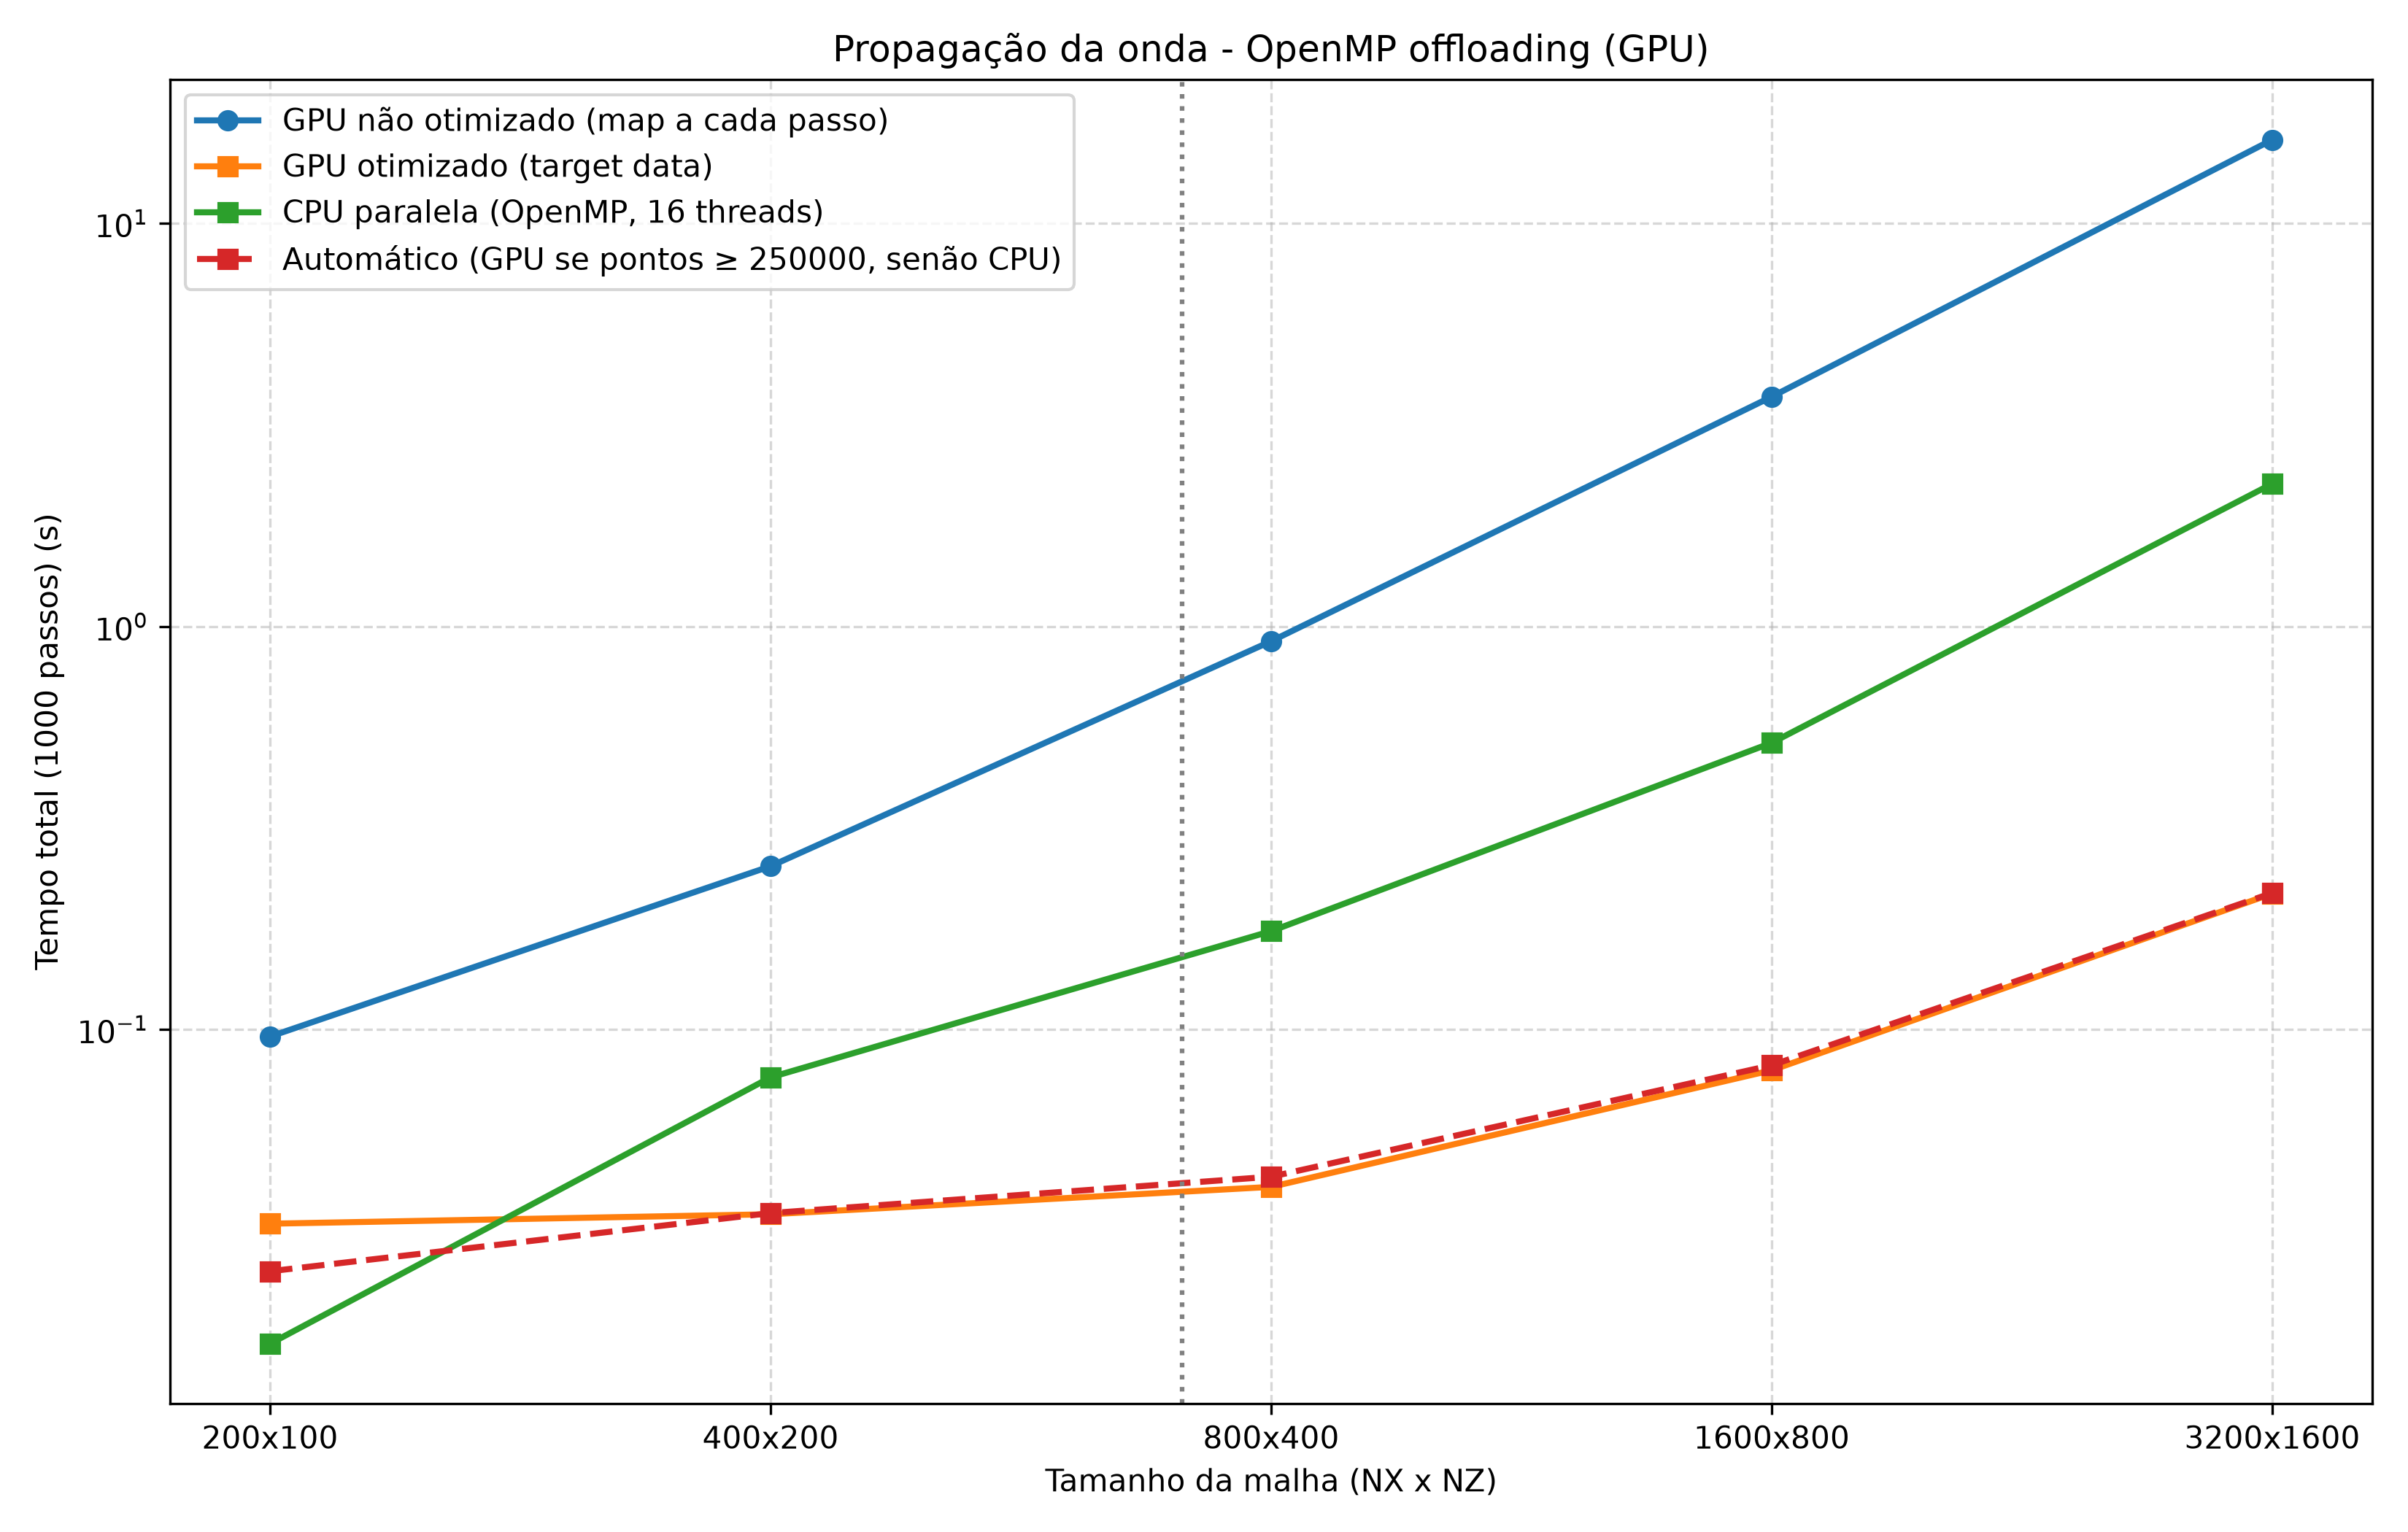
\includegraphics[width=\linewidth]{Tarefa13/tarefa13_tempos.png}
	\end{figure}
	\begin{figure}[H]
		\centering
		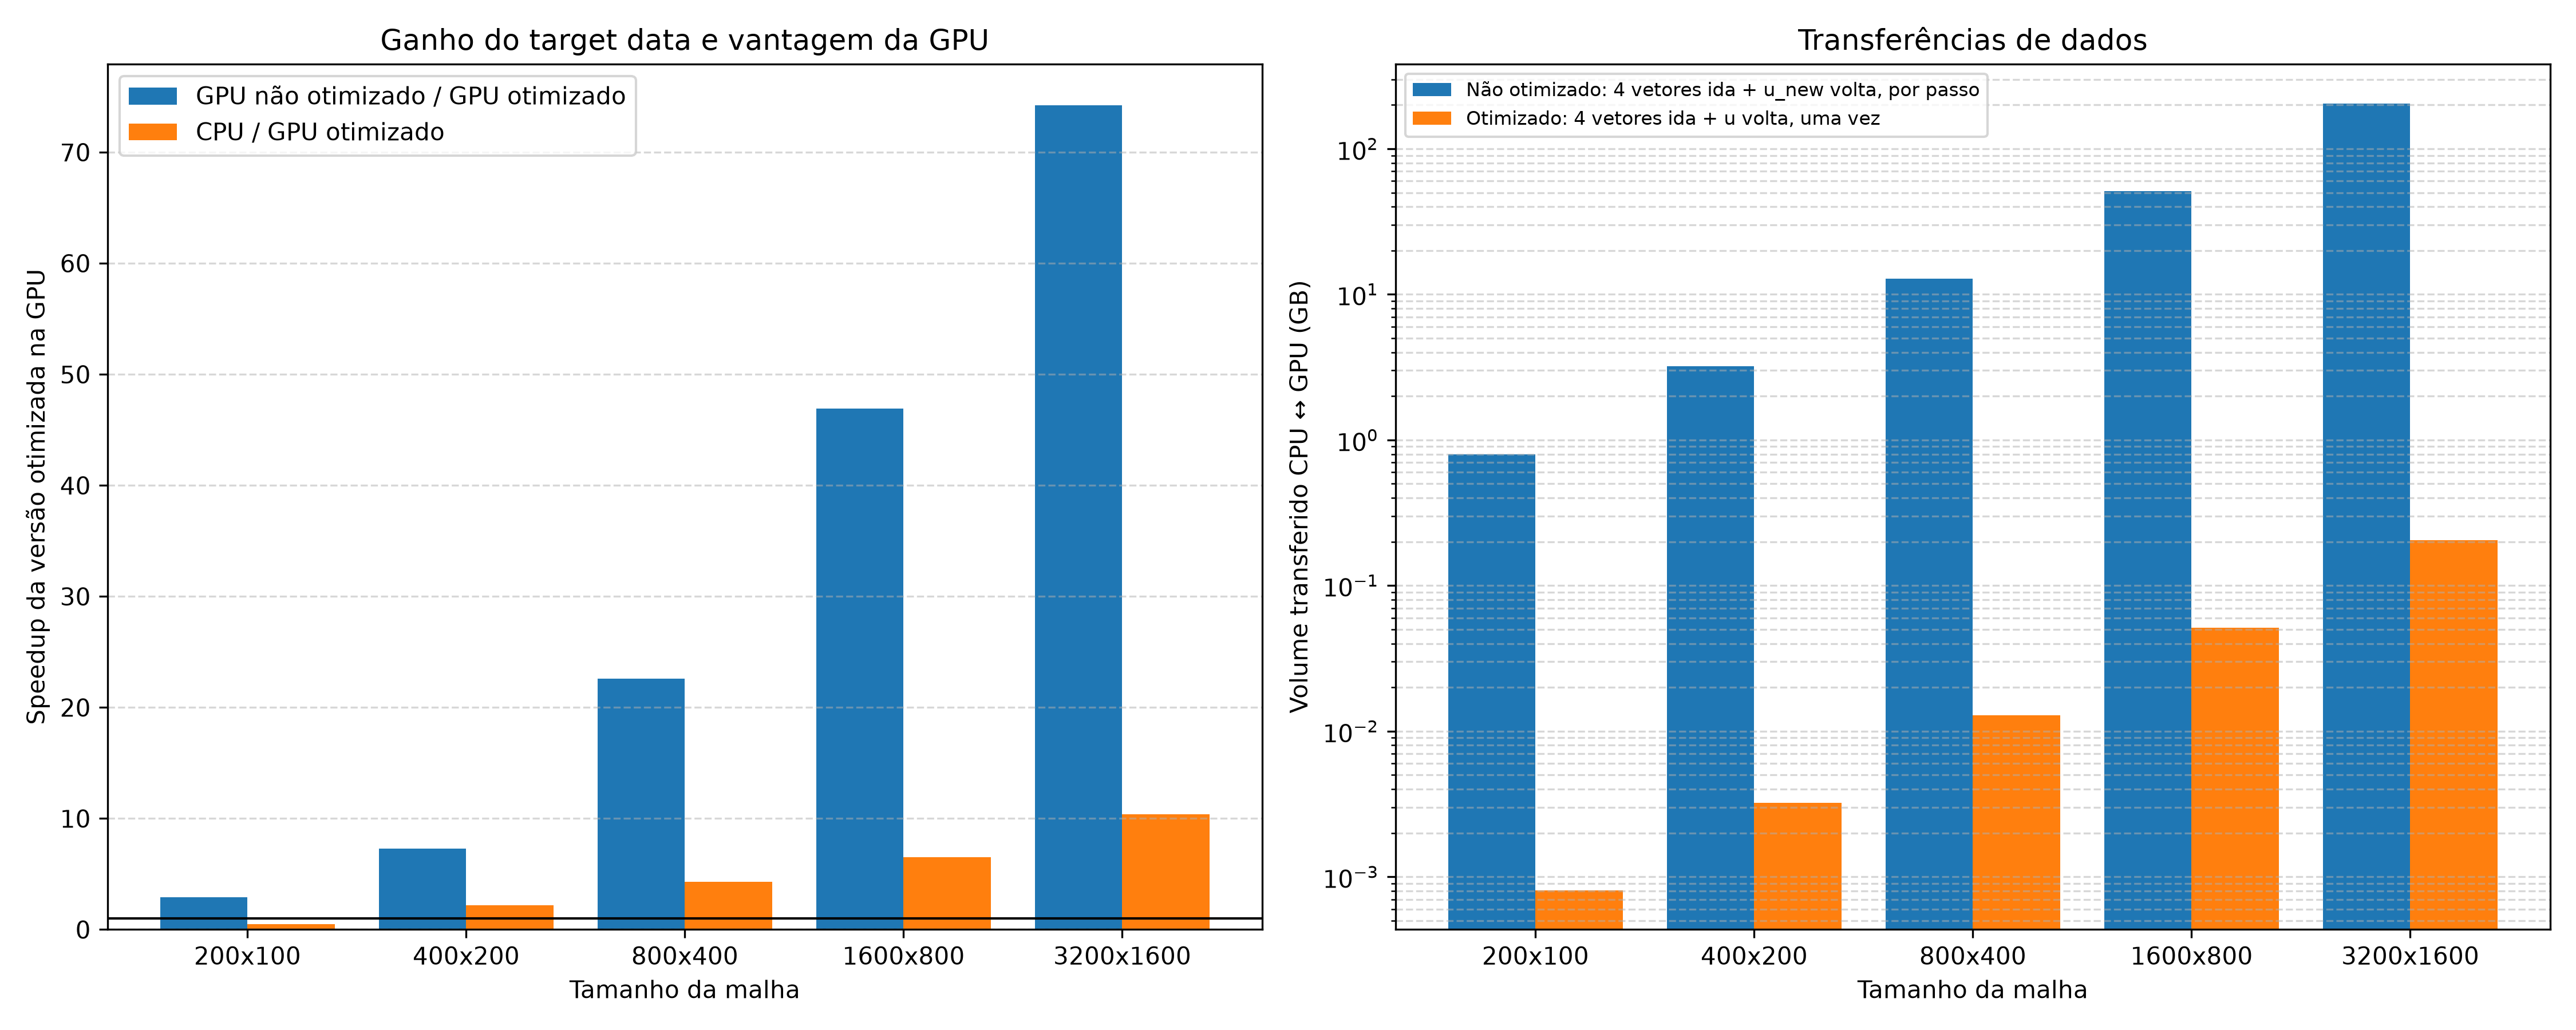
\includegraphics[width=\linewidth]{Tarefa13/tarefa13_otimizacao.png}
	\end{figure}
	\begin{figure}[H]
		\centering
		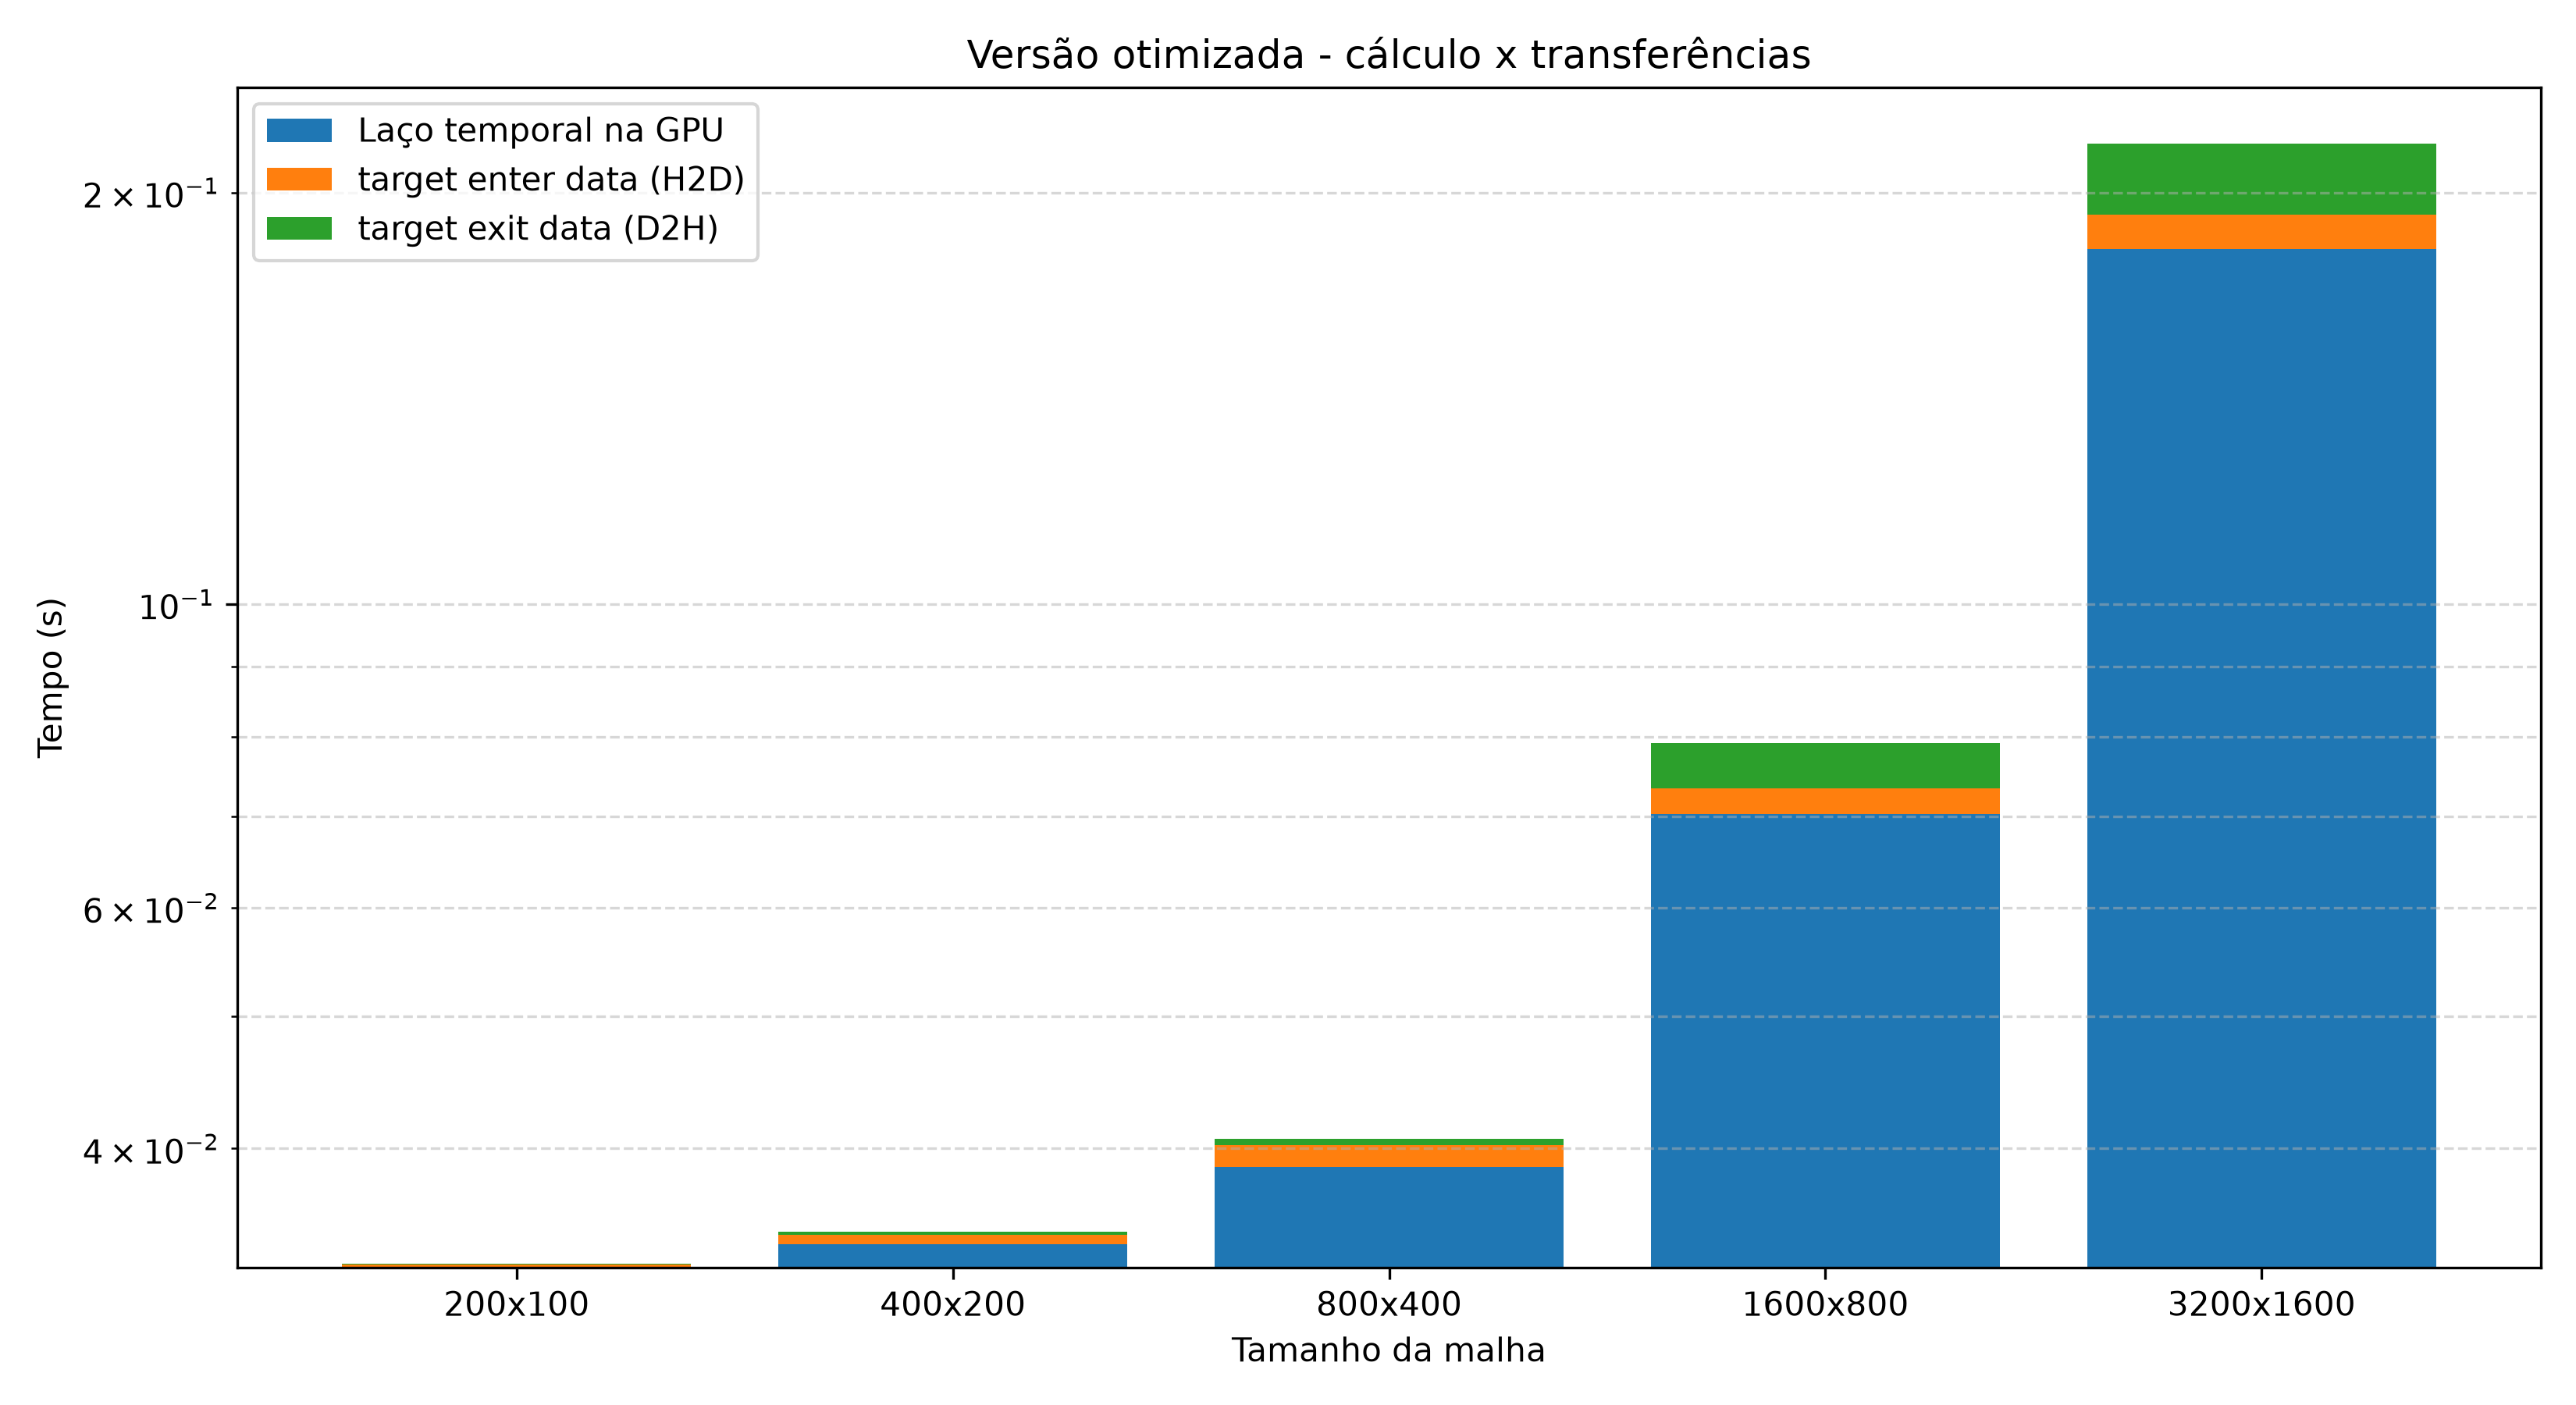
\includegraphics[width=\linewidth]{Tarefa13/tarefa13_transferencias.png}
	\end{figure}
	\par{
		Analisando os resultados, vemos que a versão não otimizada (azul) possui desempenho um pouco melhor comparado à versão com CPU (verde), porém ainda pior do que todas as alternativas para todos os números estudados.
		
		A versão otimizada demonstra ser muito mais performática do que a não otimizada, pois descarta o maior desafio de performance encontrado nesse problema: a comunicação constante entre o Host e Dispositivo. A versão não otimizada precisa receber, calcular e enviar os dados a cada passo, resultando num crescimento proporcional aos números utilizados. Utilizando otimização com target data, recebimento e envio são feitos apenas uma vez, no início e fim do cálculo, permitindo foco dos recursos na tarefa em si.
		
		A versão otimizada com target data se mostra a melhor para números maiores, porém em malhas pequenas performa pior do que a versão em CPU com paralelização por OpenMP, o que se dá devido ao overhead de inicialização. Como todos os dados são enviados para a GPU logo de início (um custo que varia de acordo com a taxa de transferência do meio e tamanho dos dados a serem enviados), para malhas pequenas como 200x100, esse custo é quase o mesmo tempo do cálculo na GPU, o que torna esse método inefetivo em otimizar o problema.
		
		Portanto, podemos optar por usar um modo híbrido, que utiliza a paralelização em CPU para números pequenos, optando pela versão otimizada em GPU a partir do ponto em que o overhead passa a ser descartável.
	}
	\subsection{\subtTres}
	\begin{lstlisting}[language=c, title=main.c]
#include <stdio.h>
#include <stdlib.h>
#include <math.h>
#include <omp.h>

#pragma omp declare target
static int NX = 200;
static int NZ = 100;
#pragma omp end declare target

static const size_t tamanhos[] = {200, 400, 800, 1600, 3200};
#define NUM_TAMANHOS (sizeof(tamanhos) / sizeof(tamanhos[0]))

static int salvar_campo = 0;
static double soma_receptor = 0.0;

#define DX 10.0
#define DZ 10.0

#define DT 0.001
#define NT 1000

#define VELOCIDADE 2000.0

#define SX 100
#define SZ 50

#define RX 150
#define RZ 50

#define PI 3.14159265358979323846

double ricker(double t, double f0)
{
    double t0 = 1.0 / f0;

    double x = PI * f0 * (t - t0);

    return (1.0 - 2.0 * x * x) * exp(-x * x);
}

void inicializa_modelo(double *vel)
{
    for (int iz = 0; iz < NZ; iz++)
    {
        for (int ix = 0; ix < NX; ix++)
        {

            vel[iz * NX + ix] = VELOCIDADE;
        }
    }
}

void salva_binario(
    const char *nome,
    double *campo)
{
    FILE *fp = fopen(nome, "wb");

    if (fp == NULL)
    {
        perror("Erro ao abrir arquivo");
        exit(EXIT_FAILURE);
    }

    fwrite(
        campo,
        sizeof(double),
        NX * NZ,
        fp);

    fclose(fp);
}

static double simula(void)
{

    double *vel = malloc(NX * NZ * sizeof(double));

    double *u = calloc(NX * NZ, sizeof(double));

    double *u_old = calloc(NX * NZ, sizeof(double));

    double *u_new = calloc(NX * NZ, sizeof(double));

    if (!vel || !u || !u_old || !u_new)
    {
        printf("Erro de alocacao de memoria\n");
        exit(EXIT_FAILURE);
    }

    inicializa_modelo(vel);

    FILE *receiver = fopen("receiver.dat", "w");

    if (receiver == NULL)
    {
        printf("Erro ao abrir receiver.dat\n");
        exit(EXIT_FAILURE);
    }

    double f0 = 20.0;

    double dt2 = DT * DT;

    soma_receptor = 0.0;
    double inicio = omp_get_wtime();

    for (int it = 0; it < NT; it++)
    {

        double t = it * DT;

#pragma omp target teams distribute parallel for collapse(2)       \
    map(to : u[0 : NX * NZ], u_old[0 : NX * NZ], vel[0 : NX * NZ]) \
    map(tofrom : u_new[0 : NX * NZ])
        for (int iz = 1; iz < NZ - 1; iz++)
        {

            for (int ix = 1; ix < NX - 1; ix++)
            {

                int id = iz * NX + ix;

                double d2udx2 =
                    (u[id + 1] - 2.0 * u[id] + u[id - 1]) / (DX * DX);

                double d2udz2 =
                    (u[id + NX] - 2.0 * u[id] + u[id - NX]) / (DZ * DZ);

                u_new[id] =
                    2.0 * u[id] - u_old[id] + vel[id] * vel[id] * dt2 * (d2udx2 + d2udz2);
            }
        }

        int source_id = SZ * NX + SX;

        u_new[source_id] += ricker(t, f0);

        int receiver_id = RZ * NX + RX;

        fprintf(
            receiver,
            "%lf %lf\n",
            t,
            u_new[receiver_id]);

        soma_receptor += fabs(u_new[receiver_id]);

        char nome[100];

        sprintf(
            nome,
            "wavefield_%04d.bin",
            it);

        if (salvar_campo)
            salva_binario(nome, u_new);

        double *tmp;

        tmp = u_old;
        u_old = u;

        u = u_new;

        u_new = tmp;

        if (it % 100 == 0)
        {
            printf(
                "Passo %d / %d\n",
                it,
                NT);
        }
    }

    double tempo = omp_get_wtime() - inicio;

    fclose(receiver);

    free(vel);
    free(u);
    free(u_old);
    free(u_new);

    printf("\nSimulacao finalizada.\n");

    return tempo;
}

int main(int argc, char *argv[])
{
    if (argc > 1)
        salvar_campo = atoi(argv[1]);

#pragma omp target
    {
    }

    FILE *saida = fopen("resultados_nao_otimizado.json", "w");

    if (saida == NULL)
        return 1;

    fprintf(saida, "{\n  \"versao\": \"nao_otimizado\",\n  \"dispositivos\": %d,\n"
                   "  \"threads\": %d,\n  \"nt\": %d,\n  \"resultados\": [\n",
            omp_get_num_devices(), omp_get_max_threads(), NT);

    for (size_t i = 0; i < NUM_TAMANHOS; i++)
    {
        NX = (int)tamanhos[i];
        NZ = (int)tamanhos[i] / 2;
#pragma omp target update to(NX, NZ)

        double tempo = simula();

        printf("[NAO OTIMIZADO] %dx%d: %.6f s\n", NX, NZ, tempo);

        fprintf(saida,
                "    {\"nx\": %d, \"nz\": %d, \"modo\": \"gpu_map\", \"tempo_total_s\": %.6f, "
                "\"soma_receptor\": %.10e}%s\n",
                NX, NZ, tempo, soma_receptor, i + 1 < NUM_TAMANHOS ? "," : "");
        fflush(saida);
        fflush(stdout);
    }

    fprintf(saida, "  ]\n}\n");
    fclose(saida);

    return 0;
}
\end{lstlisting}
	\begin{lstlisting}[language=c, title=main\_otimizado.c]
#include <stdio.h>
#include <stdlib.h>
#include <math.h>
#include <omp.h>

#pragma omp declare target
static int NX = 200;
static int NZ = 100;
#pragma omp end declare target

static const size_t tamanhos[] = {200, 400, 800, 1600, 3200};
#define NUM_TAMANHOS (sizeof(tamanhos) / sizeof(tamanhos[0]))

static int salvar_campo = 0;
static double soma_receptor = 0.0;
static long limiar_gpu = 250000;
static double tempo_h2d = 0.0;
static double tempo_d2h = 0.0;

#define DX 10.0
#define DZ 10.0

#define DT 0.001
#define NT 1000

#define VELOCIDADE 2000.0

#define SX 100
#define SZ 50

#define RX 150
#define RZ 50

#define PI 3.14159265358979323846

double ricker(double t, double f0)
{
    double t0 = 1.0 / f0;

    double x = PI * f0 * (t - t0);

    return (1.0 - 2.0 * x * x) * exp(-x * x);
}

void inicializa_modelo(double *vel)
{
    for (int iz = 0; iz < NZ; iz++)
    {
        for (int ix = 0; ix < NX; ix++)
        {

            vel[iz * NX + ix] = VELOCIDADE;
        }
    }
}

void salva_binario(
    const char *nome,
    double *campo)
{
    FILE *fp = fopen(nome, "wb");

    if (fp == NULL)
    {
        perror("Erro ao abrir arquivo");
        exit(EXIT_FAILURE);
    }

    fwrite(
        campo,
        sizeof(double),
        NX * NZ,
        fp);

    fclose(fp);
}

static double simula(void)
{

    double *vel = malloc(NX * NZ * sizeof(double));

    double *u = calloc(NX * NZ, sizeof(double));

    double *u_old = calloc(NX * NZ, sizeof(double));

    double *u_new = calloc(NX * NZ, sizeof(double));

    if (!vel || !u || !u_old || !u_new)
    {
        printf("Erro de alocacao de memoria\n");
        exit(EXIT_FAILURE);
    }

    inicializa_modelo(vel);

    FILE *receiver = fopen("receiver.dat", "w");

    if (receiver == NULL)
    {
        printf("Erro ao abrir receiver.dat\n");
        exit(EXIT_FAILURE);
    }

    double f0 = 20.0;

    double dt2 = DT * DT;

    soma_receptor = 0.0;
    int usa_gpu = (long)NX * NZ >= limiar_gpu;

    double inicio = omp_get_wtime();

#pragma omp target enter data if(usa_gpu)                         \
    map(to : vel[0 : NX * NZ], u[0 : NX * NZ], u_old[0 : NX * NZ], \
            u_new[0 : NX * NZ])

    tempo_h2d = omp_get_wtime() - inicio;

    for (int it = 0; it < NT; it++)
    {

        double t = it * DT;

        if (usa_gpu)
        {
#pragma omp target teams distribute parallel for collapse(2)
            for (int iz = 1; iz < NZ - 1; iz++)
            {

                for (int ix = 1; ix < NX - 1; ix++)
                {

                    int id = iz * NX + ix;

                    double d2udx2 =
                        (u[id + 1] - 2.0 * u[id] + u[id - 1]) / (DX * DX);

                    double d2udz2 =
                        (u[id + NX] - 2.0 * u[id] + u[id - NX]) / (DZ * DZ);

                    u_new[id] =
                        2.0 * u[id] - u_old[id] + vel[id] * vel[id] * dt2 * (d2udx2 + d2udz2);
                }
            }
        }
        else
        {
#pragma omp parallel for collapse(2)
            for (int iz = 1; iz < NZ - 1; iz++)
            {

                for (int ix = 1; ix < NX - 1; ix++)
                {

                    int id = iz * NX + ix;

                    double d2udx2 =
                        (u[id + 1] - 2.0 * u[id] + u[id - 1]) / (DX * DX);

                    double d2udz2 =
                        (u[id + NX] - 2.0 * u[id] + u[id - NX]) / (DZ * DZ);

                    u_new[id] =
                        2.0 * u[id] - u_old[id] + vel[id] * vel[id] * dt2 * (d2udx2 + d2udz2);
                }
            }
        }

        int source_id = SZ * NX + SX;

        double fonte = ricker(t, f0);

#pragma omp target if(usa_gpu)
        u_new[source_id] += fonte;

        int receiver_id = RZ * NX + RX;

#pragma omp target update if(usa_gpu) from(u_new[receiver_id : 1])

        fprintf(
            receiver,
            "%lf %lf\n",
            t,
            u_new[receiver_id]);

        soma_receptor += fabs(u_new[receiver_id]);

        char nome[100];

        sprintf(
            nome,
            "wavefield_%04d.bin",
            it);

        if (salvar_campo)
        {
#pragma omp target update if(usa_gpu) from(u_new[0 : NX * NZ])
            salva_binario(nome, u_new);
        }

        double *tmp;

        tmp = u_old;
        u_old = u;

        u = u_new;

        u_new = tmp;

        if (it % 100 == 0)
        {
            printf(
                "Passo %d / %d\n",
                it,
                NT);
        }
    }

    double inicio_d2h = omp_get_wtime();

#pragma omp target exit data if(usa_gpu) map(from : u[0 : NX * NZ]) \
    map(release : vel[0 : NX * NZ], u_old[0 : NX * NZ], u_new[0 : NX * NZ])

    tempo_d2h = omp_get_wtime() - inicio_d2h;

    double tempo = omp_get_wtime() - inicio;

    fclose(receiver);

    free(vel);
    free(u);
    free(u_old);
    free(u_new);

    printf("\nSimulacao finalizada.\n");

    return tempo;
}

int main(int argc, char *argv[])
{
    if (argc > 1)
        salvar_campo = atoi(argv[1]);

    const char *env_limiar = getenv("LIMIAR_GPU");
    long limiar_auto = env_limiar ? atol(env_limiar) : limiar_gpu;

#pragma omp target
    {
    }

    FILE *saida = fopen("resultados_otimizado.json", "w");

    if (saida == NULL)
        return 1;

    fprintf(saida, "{\n  \"versao\": \"otimizado\",\n  \"dispositivos\": %d,\n"
                   "  \"threads\": %d,\n  \"nt\": %d,\n  \"limiar_gpu\": %ld,\n"
                   "  \"resultados\": [\n",
            omp_get_num_devices(), omp_get_max_threads(), NT, limiar_auto);

    const char *modos[] = {"auto", "gpu", "cpu"};
    const long limiares[] = {limiar_auto, 0, -1};
    int primeiro = 1;

    for (size_t i = 0; i < NUM_TAMANHOS; i++)
    {
        NX = (int)tamanhos[i];
        NZ = (int)tamanhos[i] / 2;
#pragma omp target update to(NX, NZ)

        for (int m = 0; m < 3; m++)
        {
            limiar_gpu = limiares[m] < 0 ? (long)NX * NZ + 1 : limiares[m];
            int usa_gpu = (long)NX * NZ >= limiar_gpu;

            double tempo = simula();

            printf("[OTIMIZADO %s] %dx%d (%s): %.6f s | H2D %.6f s | D2H %.6f s\n",
                   modos[m], NX, NZ, usa_gpu ? "gpu" : "cpu", tempo, tempo_h2d, tempo_d2h);

            fprintf(saida,
                    "%s    {\"nx\": %d, \"nz\": %d, \"modo\": \"%s\", \"executou_em\": \"%s\", "
                    "\"tempo_total_s\": %.6f, \"tempo_h2d_s\": %.6f, \"tempo_d2h_s\": %.6f, "
                    "\"soma_receptor\": %.10e}",
                    primeiro ? "" : ",\n", NX, NZ, modos[m], usa_gpu ? "gpu" : "cpu",
                    tempo, tempo_h2d, tempo_d2h, soma_receptor);
            primeiro = 0;
            fflush(saida);
            fflush(stdout);
        }
    }

    fprintf(saida, "\n  ]\n}\n");
    fclose(saida);

    return 0;
}
\end{lstlisting}
	\begin{lstlisting}[language=bash, title=script\_gpu.sh]
#!/bin/bash
#SBATCH --job-name=OMP_GPU_onda_akira
#SBATCH --output=saida%j.out
#SBATCH --error=erro%j.err
#SBATCH --partition=gpu-4-a100
#SBATCH --nodes=1
#SBATCH --ntasks=1
#SBATCH --cpus-per-task=16
#SBATCH --gpus-per-node=1
#SBATCH --time=0-0:30

cd "${SLURM_SUBMIT_DIR:-.}"
mkdir -p outputs
export OMP_NUM_THREADS=${SLURM_CPUS_PER_TASK:-16}

nvidia-smi --query-gpu=name,memory.total --format=csv 2> /dev/null

carrega_nvhpc() {
    command -v nvc > /dev/null 2>&1 && return 0
    if ! type module > /dev/null 2>&1; then
        for f in /etc/profile.d/modules.sh /etc/profile.d/lmod.sh /usr/share/lmod/lmod/init/bash; do
            [ -f "$f" ] && source "$f" && break
        done
    fi
    type module > /dev/null 2>&1 || return 1
    local mod=${NVHPC_MODULE:-$(module -t avail 2>&1 | grep -v ':$' | grep -vE '^(containers|softwares)/' | grep -i 'nvhpc' | sort -V | tail -n 1)}
    [ -n "$mod" ] && echo "Carregando modulo: $mod" && module load "$mod"
    command -v nvc > /dev/null 2>&1
}

carrega_nvhpc

for prog in main main_otimizado; do
    if command -v nvc > /dev/null 2>&1 && nvc -O2 -mp=gpu $prog.c -o outputs/$prog 2> outputs/build_nvc.log; then
        echo "$prog: NVHPC (-mp=gpu)"
    elif gcc -O2 -fopenmp -foffload=nvptx-none -fno-stack-protector $prog.c -o outputs/$prog -lm 2> outputs/build_gcc.log; then
        echo "$prog: GCC + nvptx-none"
    else
        echo "Sem compilador com offload (veja outputs/build_*.log)" >&2
        exit 1
    fi
done

./outputs/main
./outputs/main_otimizado

if command -v python3 > /dev/null 2>&1 && python3 -c "import matplotlib" 2> /dev/null; then
    python3 plot.py
fi
\end{lstlisting}
	
	\newpage
	\onehalfspacing
	\section{TAREFA 14}
	\subsection{\subtUm}
	\par{Implementar duas versões paralelas do código de propagação de onda para GPU utilizando CUDA: uma com memória unificada e outra com gerenciamento explícito de memória.
		
		Realizar experimentos com diferentes tamanhos de problema, comparando o tempo de execução e de transferência, o impacto do tamanho do problema e os resultados com o OpenMP Offloading, identificando as situações em que o uso do CUDA é vantajoso ou não.}
	\subsection{\subtDois}
	
	\begin{figure}[H]
		\centering
		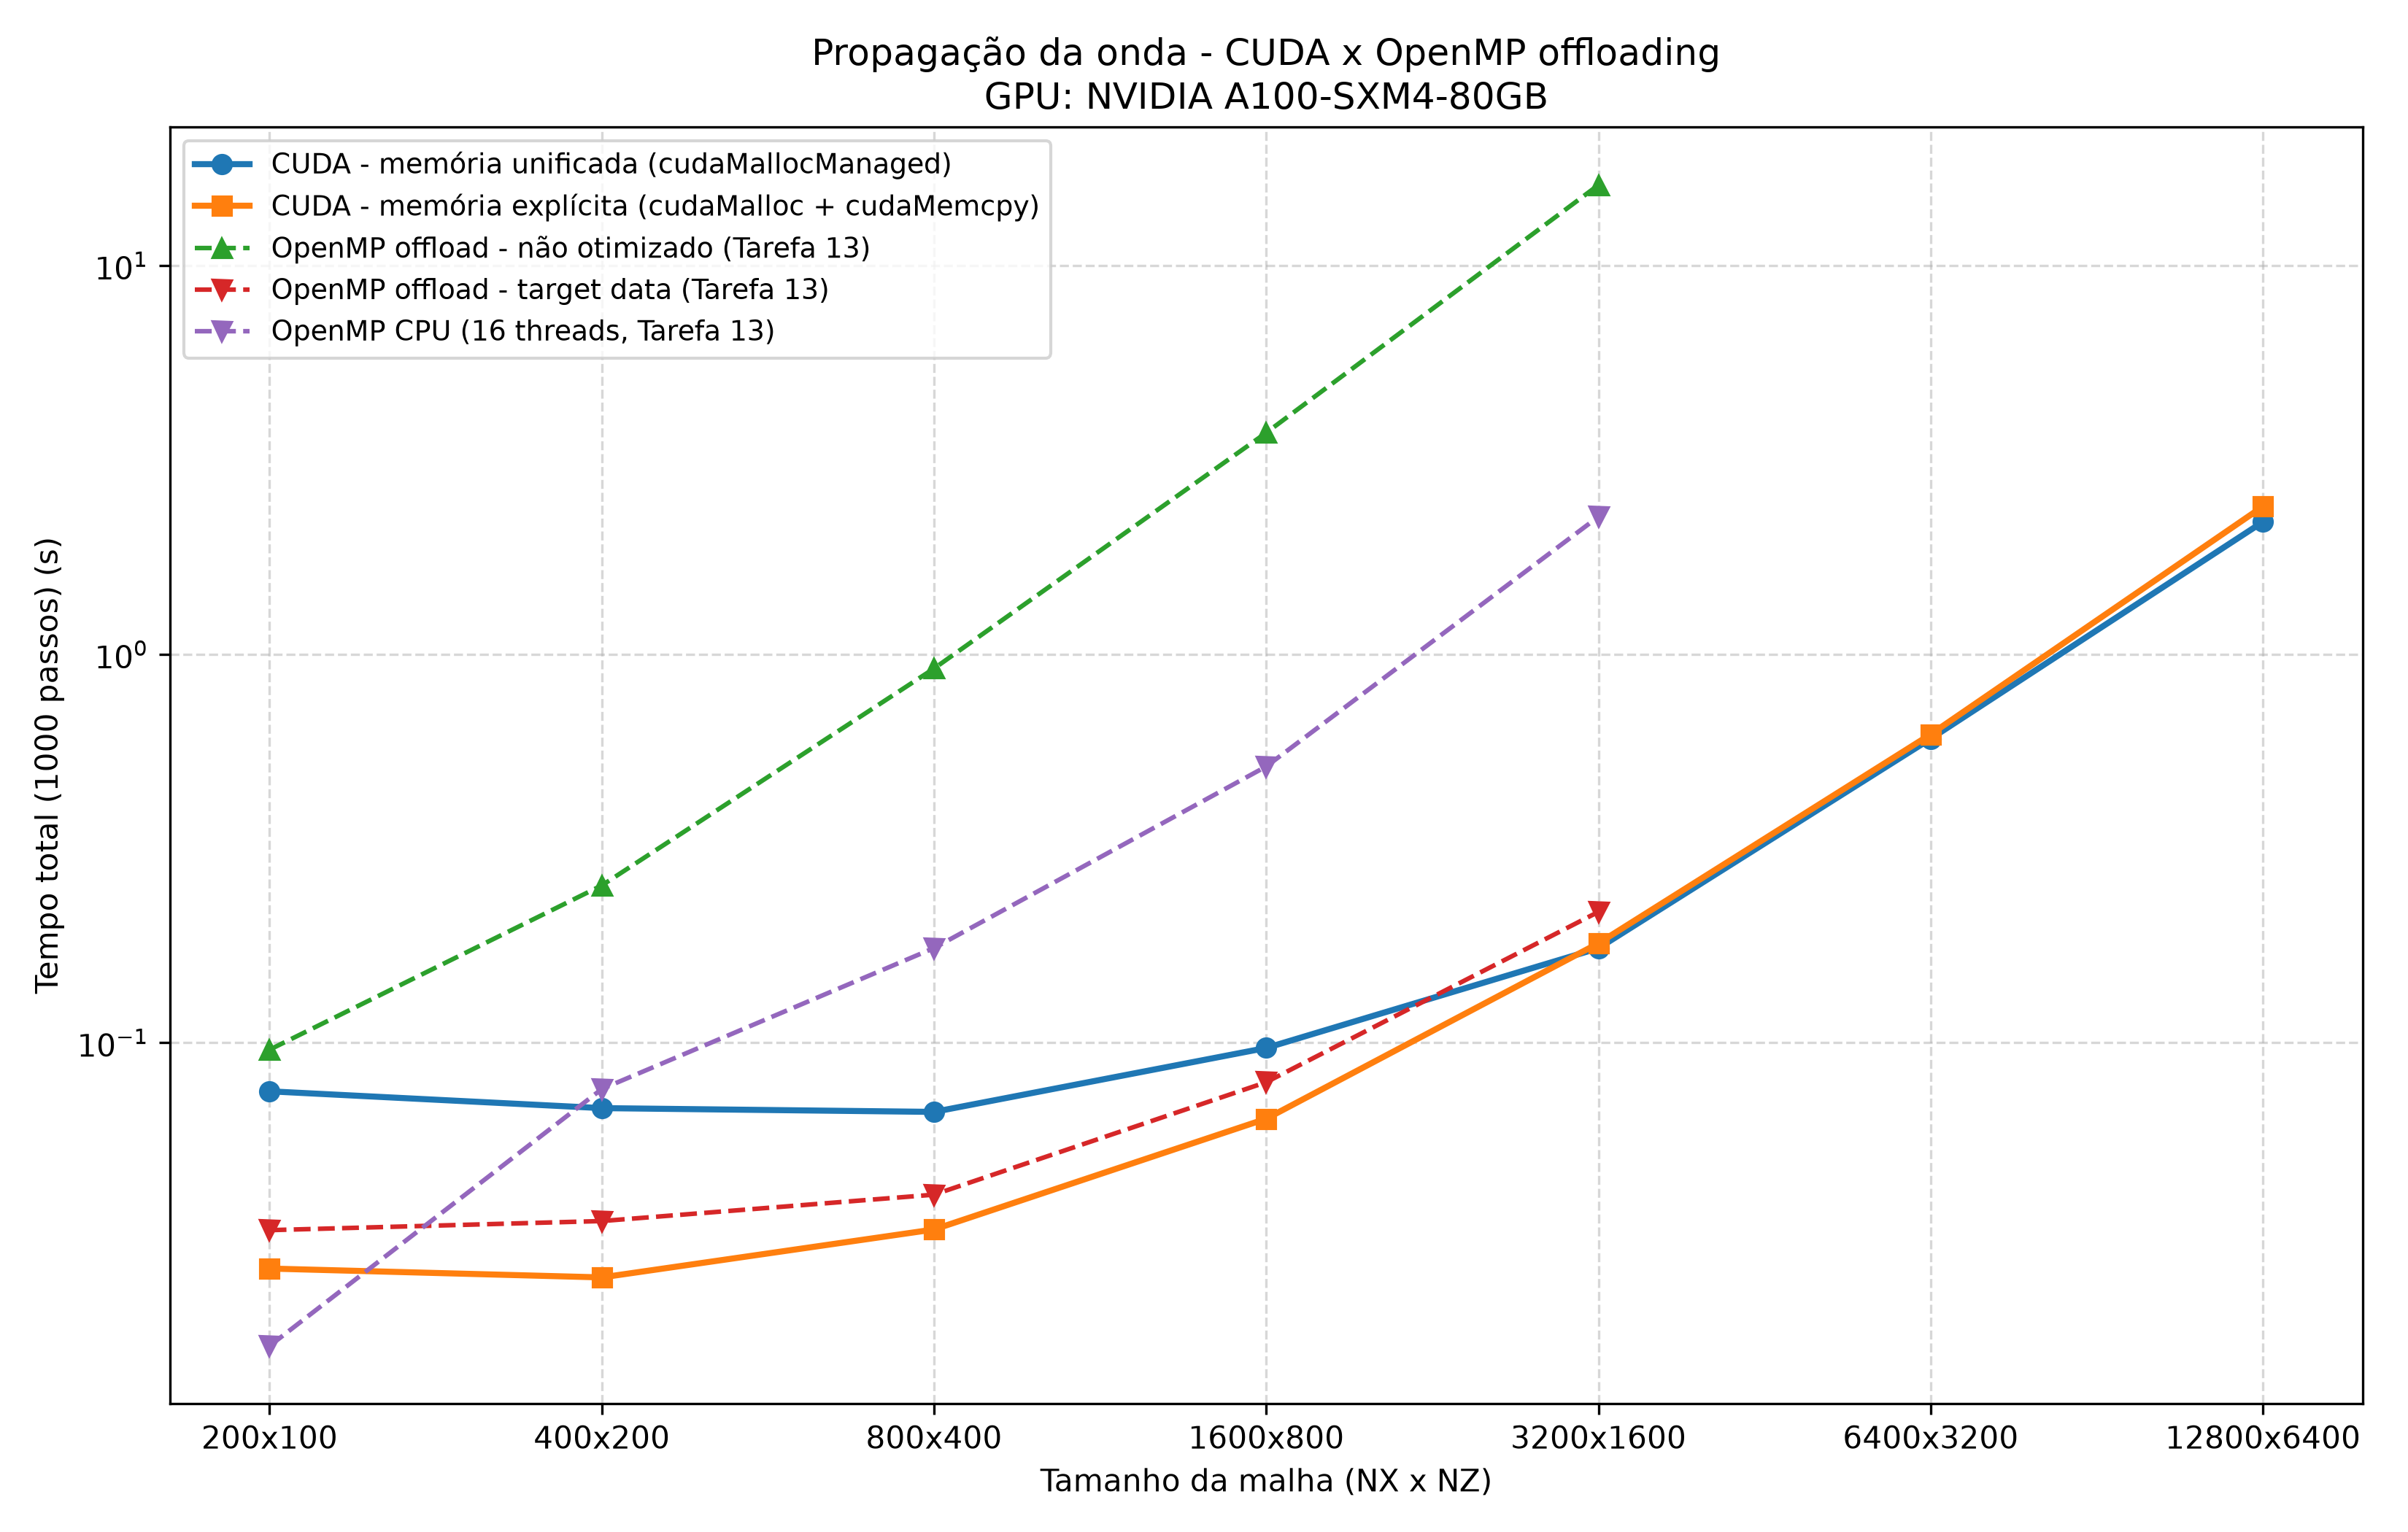
\includegraphics[width=\linewidth]{Tarefa14/tarefa14_tempos.png}
	\end{figure}
	\begin{figure}[H]
		\centering
		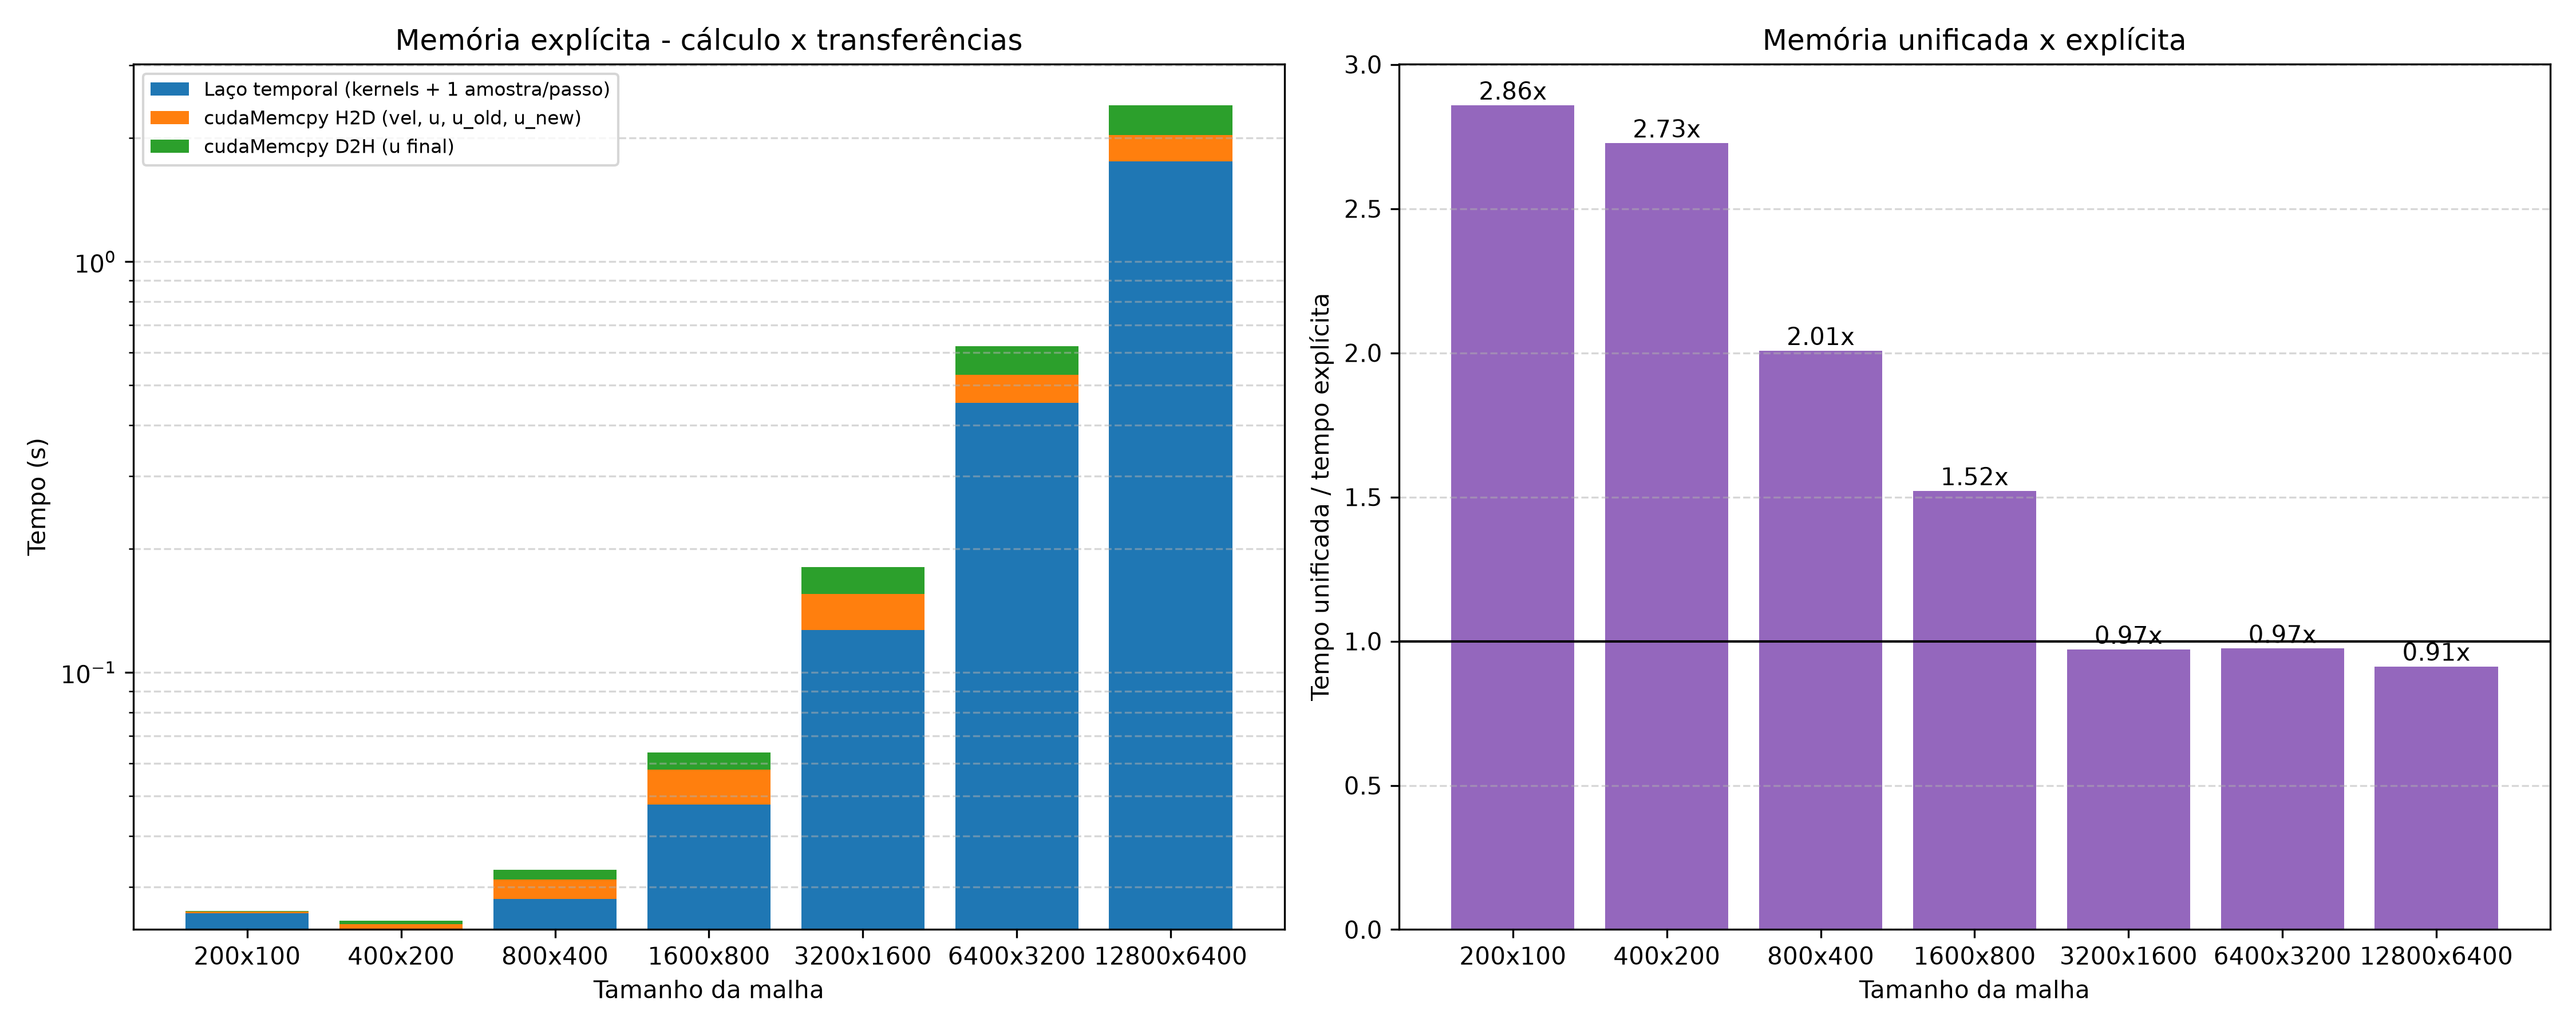
\includegraphics[width=\linewidth]{Tarefa14/tarefa14_memoria.png}
	\end{figure}
	\par{
		Analisando o gráfico de comparações entre os códigos em CUDA com memória unificada, explicita, offload em OPENMP com e sem otimização e paralelização em CPU, feito a partir do supercomputador NPAD, podemos verificar que ambas as versões com cuda se mostram mais performáticas do que todas as alternativas a partir de malhas 3200x1600.
		
		É possível notar, também, que a opção por memória unificada, apesar de iniciar mais lenta do que a opção por memória explicita, ao longo do tempo diminui a diferença entre eles, chegando a ultrapassar em performance a partir de malhas 12800x6400. Isso se dá pois a versão explícita copia mais dados do que a unificada, aumentando de acordo com o tamanho da malha, enquanto o custo extra da unificada é fixo
		
		Portanto, identificamos que as versões em CUDA são mais vantajosas quando lidando com problemas de grande escala, sendo ideal para tarefas de inteligência artificial, por exemplo.
	}
	\subsection{\subtTres}
	\begin{lstlisting}[language=c, title=wave.cu]
#include <stdio.h>
#include <stdlib.h>
#include <math.h>
#include <time.h>

static int NX = 200;
static int NZ = 100;

static const size_t tamanhos[] = {200, 400, 800, 1600, 3200, 6400, 12800};
#define NUM_TAMANHOS (sizeof(tamanhos) / sizeof(tamanhos[0]))

static int salvar_campo = 0;
static double soma_receptor = 0.0;

static double agora(void)
{
    struct timespec ts;
    clock_gettime(CLOCK_MONOTONIC, &ts);
    return ts.tv_sec + ts.tv_nsec * 1e-9;
}

#define DX 10.0
#define DZ 10.0

#define DT 0.001
#define NT 1000

#define VELOCIDADE 2000.0

#define SX 100
#define SZ 50

#define RX 150
#define RZ 50

#define PI 3.14159265358979323846

double ricker(double t, double f0)
{
    double t0 = 1.0 / f0;

    double x = PI * f0 * (t - t0);

    return (1.0 - 2.0 * x * x) * exp(-x * x);
}

void inicializa_modelo(double *vel)
{
    for (int iz = 0; iz < NZ; iz++) {
        for (int ix = 0; ix < NX; ix++) {

            vel[iz * NX + ix] = VELOCIDADE;
        }
    }
}

void salva_binario(
    const char *nome,
    double *campo)
{
    FILE *fp = fopen(nome, "wb");

    if (fp == NULL) {
        perror("Erro ao abrir arquivo");
        exit(EXIT_FAILURE);
    }

    fwrite(
        campo,
        sizeof(double),
        NX * NZ,
        fp
    );

    fclose(fp);
}

__global__ void atualiza_campo(
    const double *vel,
    const double *u,
    const double *u_old,
    double *u_new,
    double dt2,
    int NX,
    int NZ)
{
    int ix = blockIdx.x * blockDim.x + threadIdx.x;
    int iz = blockIdx.y * blockDim.y + threadIdx.y;

    if (ix >= 1 && ix < NX - 1 && iz >= 1 && iz < NZ - 1) {

        int id = iz * NX + ix;

        double d2udx2 =
            (u[id + 1]
           - 2.0 * u[id]
           + u[id - 1])
            / (DX * DX);

        double d2udz2 =
            (u[id + NX]
           - 2.0 * u[id]
           + u[id - NX])
            / (DZ * DZ);

        u_new[id] =
            2.0 * u[id]
            - u_old[id]
            + vel[id] * vel[id]
            * dt2
            * (d2udx2 + d2udz2);
    }
}

static double simula(void)
{

    double *vel = NULL;

    double *u = NULL;

    double *u_old = NULL;

    double *u_new = NULL;

    cudaMallocManaged(&vel, NX * NZ * sizeof(double));
    cudaMallocManaged(&u, NX * NZ * sizeof(double));
    cudaMallocManaged(&u_old, NX * NZ * sizeof(double));
    cudaMallocManaged(&u_new, NX * NZ * sizeof(double));

    if (!vel || !u || !u_old || !u_new) {
        printf("Erro de alocacao de memoria\n");
        exit(EXIT_FAILURE);
    }

    cudaMemset(u, 0, NX * NZ * sizeof(double));
    cudaMemset(u_old, 0, NX * NZ * sizeof(double));
    cudaMemset(u_new, 0, NX * NZ * sizeof(double));

    inicializa_modelo(vel);

    FILE *receiver = fopen("receiver.dat", "w");

    if (receiver == NULL) {
        printf("Erro ao abrir receiver.dat\n");
        exit(EXIT_FAILURE);
    }

    double f0 = 20.0;

    double dt2 = DT * DT;

    dim3 block(16, 16);
    dim3 grid((NX + block.x - 1) / block.x, (NZ + block.y - 1) / block.y);

    soma_receptor = 0.0;
    double inicio = agora();

    for (int it = 0; it < NT; it++) {

        double t = it * DT;

        atualiza_campo<<<grid, block>>>(vel, u, u_old, u_new, dt2, NX, NZ);

        cudaDeviceSynchronize();

        int source_id = SZ * NX + SX;

        u_new[source_id] += ricker(t, f0);

        int receiver_id = RZ * NX + RX;

        fprintf(
            receiver,
            "%lf %lf\n",
            t,
            u_new[receiver_id]
        );

        soma_receptor += fabs(u_new[receiver_id]);

        char nome[100];

        sprintf(
            nome,
            "wavefield_%04d.bin",
            it
        );

        if (salvar_campo)
            salva_binario(nome, u_new);

        double *tmp;

        tmp = u_old;
        u_old = u;

        u = u_new;

        u_new = tmp;

        if (it % 100 == 0) {
            printf(
                "Passo %d / %d\n",
                it,
                NT
            );
        }
    }

    double tempo = agora() - inicio;

    fclose(receiver);

    cudaFree(vel);
    cudaFree(u);
    cudaFree(u_old);
    cudaFree(u_new);

    printf("\nSimulacao finalizada.\n");

    return tempo;
}

int main(int argc, char *argv[])
{
    if (argc > 1)
        salvar_campo = atoi(argv[1]);

    cudaFree(0);

    cudaDeviceProp prop;
    cudaGetDeviceProperties(&prop, 0);

    FILE *saida = fopen("resultados_unificada.json", "w");

    if (saida == NULL)
        return 1;

    fprintf(saida, "{\n  \"versao\": \"memoria_unificada\",\n  \"gpu\": \"%s\",\n"
                   "  \"nt\": %d,\n  \"resultados\": [\n", prop.name, NT);

    for (size_t i = 0; i < NUM_TAMANHOS; i++) {
        NX = (int)tamanhos[i];
        NZ = (int)tamanhos[i] / 2;

        double tempo = simula();

        printf("[UNIFICADA] %dx%d: %.6f s\n", NX, NZ, tempo);

        fprintf(saida,
                "    {\"nx\": %d, \"nz\": %d, \"tempo_total_s\": %.6f, "
                "\"soma_receptor\": %.10e}%s\n",
                NX, NZ, tempo, soma_receptor, i + 1 < NUM_TAMANHOS ? "," : "");
    }

    fprintf(saida, "  ]\n}\n");
    fclose(saida);

    return 0;
}
\end{lstlisting}
	\begin{lstlisting}[language=c, title=wave\_explicito.cu]
#include <stdio.h>
#include <stdlib.h>
#include <math.h>
#include <time.h>

static int NX = 200;
static int NZ = 100;

static const size_t tamanhos[] = {200, 400, 800, 1600, 3200, 6400, 12800};
#define NUM_TAMANHOS (sizeof(tamanhos) / sizeof(tamanhos[0]))

static int salvar_campo = 0;
static double soma_receptor = 0.0;
static double tempo_h2d = 0.0;
static double tempo_d2h = 0.0;

static double agora(void)
{
    struct timespec ts;
    clock_gettime(CLOCK_MONOTONIC, &ts);
    return ts.tv_sec + ts.tv_nsec * 1e-9;
}

#define DX 10.0
#define DZ 10.0

#define DT 0.001
#define NT 1000

#define VELOCIDADE 2000.0

#define SX 100
#define SZ 50

#define RX 150
#define RZ 50

#define PI 3.14159265358979323846

double ricker(double t, double f0)
{
    double t0 = 1.0 / f0;

    double x = PI * f0 * (t - t0);

    return (1.0 - 2.0 * x * x) * exp(-x * x);
}

void inicializa_modelo(double *vel)
{
    for (int iz = 0; iz < NZ; iz++) {
        for (int ix = 0; ix < NX; ix++) {

            vel[iz * NX + ix] = VELOCIDADE;
        }
    }
}

void salva_binario(
    const char *nome,
    double *campo)
{
    FILE *fp = fopen(nome, "wb");

    if (fp == NULL) {
        perror("Erro ao abrir arquivo");
        exit(EXIT_FAILURE);
    }

    fwrite(
        campo,
        sizeof(double),
        NX * NZ,
        fp
    );

    fclose(fp);
}

__global__ void atualiza_campo(
    const double *vel,
    const double *u,
    const double *u_old,
    double *u_new,
    double dt2,
    int NX,
    int NZ)
{
    int ix = blockIdx.x * blockDim.x + threadIdx.x;
    int iz = blockIdx.y * blockDim.y + threadIdx.y;

    if (ix >= 1 && ix < NX - 1 && iz >= 1 && iz < NZ - 1) {

        int id = iz * NX + ix;

        double d2udx2 =
            (u[id + 1]
           - 2.0 * u[id]
           + u[id - 1])
            / (DX * DX);

        double d2udz2 =
            (u[id + NX]
           - 2.0 * u[id]
           + u[id - NX])
            / (DZ * DZ);

        u_new[id] =
            2.0 * u[id]
            - u_old[id]
            + vel[id] * vel[id]
            * dt2
            * (d2udx2 + d2udz2);
    }
}

__global__ void injeta_fonte(double *u_new, int source_id, double valor)
{
    u_new[source_id] += valor;
}

static double simula(void)
{

    double *vel = NULL;

    double *u = NULL;

    double *u_old = NULL;

    double *u_new = NULL;

    vel = (double *)malloc(NX * NZ * sizeof(double));
    u = (double *)calloc(NX * NZ, sizeof(double));
    u_old = (double *)calloc(NX * NZ, sizeof(double));
    u_new = (double *)calloc(NX * NZ, sizeof(double));

    double *d_vel = NULL, *d_u = NULL, *d_u_old = NULL, *d_u_new = NULL;

    cudaMalloc(&d_vel, NX * NZ * sizeof(double));
    cudaMalloc(&d_u, NX * NZ * sizeof(double));
    cudaMalloc(&d_u_old, NX * NZ * sizeof(double));
    cudaMalloc(&d_u_new, NX * NZ * sizeof(double));

    if (!vel || !u || !u_old || !u_new || !d_vel || !d_u || !d_u_old || !d_u_new) {
        printf("Erro de alocacao de memoria\n");
        exit(EXIT_FAILURE);
    }

    inicializa_modelo(vel);

    FILE *receiver = fopen("receiver.dat", "w");

    if (receiver == NULL) {
        printf("Erro ao abrir receiver.dat\n");
        exit(EXIT_FAILURE);
    }

    double f0 = 20.0;

    double dt2 = DT * DT;

    dim3 block(16, 16);
    dim3 grid((NX + block.x - 1) / block.x, (NZ + block.y - 1) / block.y);

    soma_receptor = 0.0;
    double inicio = agora();

    cudaMemcpy(d_vel, vel, NX * NZ * sizeof(double), cudaMemcpyHostToDevice);
    cudaMemcpy(d_u, u, NX * NZ * sizeof(double), cudaMemcpyHostToDevice);
    cudaMemcpy(d_u_old, u_old, NX * NZ * sizeof(double), cudaMemcpyHostToDevice);
    cudaMemcpy(d_u_new, u_new, NX * NZ * sizeof(double), cudaMemcpyHostToDevice);

    tempo_h2d = agora() - inicio;

    for (int it = 0; it < NT; it++) {

        double t = it * DT;

        atualiza_campo<<<grid, block>>>(d_vel, d_u, d_u_old, d_u_new, dt2, NX, NZ);

        cudaDeviceSynchronize();

        int source_id = SZ * NX + SX;

        injeta_fonte<<<1, 1>>>(d_u_new, source_id, ricker(t, f0));

        int receiver_id = RZ * NX + RX;

        double amostra;
        cudaMemcpy(&amostra, d_u_new + receiver_id, sizeof(double), cudaMemcpyDeviceToHost);

        fprintf(
            receiver,
            "%lf %lf\n",
            t,
            amostra
        );

        soma_receptor += fabs(amostra);

        char nome[100];

        sprintf(
            nome,
            "wavefield_%04d.bin",
            it
        );

        if (salvar_campo) {
            cudaMemcpy(u_new, d_u_new, NX * NZ * sizeof(double), cudaMemcpyDeviceToHost);
            salva_binario(nome, u_new);
        }

        double *tmp;

        tmp = u_old;
        u_old = u;

        u = u_new;

        u_new = tmp;

        tmp = d_u_old;
        d_u_old = d_u;
        d_u = d_u_new;
        d_u_new = tmp;

        if (it % 100 == 0) {
            printf(
                "Passo %d / %d\n",
                it,
                NT
            );
        }
    }

    double inicio_d2h = agora();

    cudaMemcpy(u, d_u, NX * NZ * sizeof(double), cudaMemcpyDeviceToHost);

    tempo_d2h = agora() - inicio_d2h;

    double tempo = agora() - inicio;

    fclose(receiver);

    cudaFree(d_vel);
    cudaFree(d_u);
    cudaFree(d_u_old);
    cudaFree(d_u_new);
    free(vel);
    free(u);
    free(u_old);
    free(u_new);

    printf("\nSimulacao finalizada.\n");

    return tempo;
}

int main(int argc, char *argv[])
{
    if (argc > 1)
        salvar_campo = atoi(argv[1]);

    cudaFree(0);

    cudaDeviceProp prop;
    cudaGetDeviceProperties(&prop, 0);

    FILE *saida = fopen("resultados_explicita.json", "w");

    if (saida == NULL)
        return 1;

    fprintf(saida, "{\n  \"versao\": \"memoria_explicita\",\n  \"gpu\": \"%s\",\n"
                   "  \"nt\": %d,\n  \"resultados\": [\n", prop.name, NT);

    for (size_t i = 0; i < NUM_TAMANHOS; i++) {
        NX = (int)tamanhos[i];
        NZ = (int)tamanhos[i] / 2;

        double tempo = simula();

        printf("[EXPLICITA] %dx%d: %.6f s | H2D %.6f s | D2H %.6f s\n",
               NX, NZ, tempo, tempo_h2d, tempo_d2h);

        fprintf(saida,
                "    {\"nx\": %d, \"nz\": %d, \"tempo_total_s\": %.6f, "
                "\"tempo_h2d_s\": %.6f, \"tempo_d2h_s\": %.6f, "
                "\"soma_receptor\": %.10e}%s\n",
                NX, NZ, tempo, tempo_h2d, tempo_d2h, soma_receptor,
                i + 1 < NUM_TAMANHOS ? "," : "");
    }

    fprintf(saida, "  ]\n}\n");
    fclose(saida);

    return 0;
}
\end{lstlisting}
	\begin{lstlisting}[language=bash, title=script\_cuda.sh]
#!/bin/bash
#SBATCH --job-name=CUDA_onda_akira
#SBATCH --output=saida%j.out
#SBATCH --error=erro%j.err
#SBATCH --partition=gpu-4-a100
#SBATCH --nodes=1
#SBATCH --ntasks=1
#SBATCH --cpus-per-task=1
#SBATCH --gpus-per-node=1
#SBATCH --time=0-0:20

cd "${SLURM_SUBMIT_DIR:-.}"
mkdir -p outputs

carrega_cuda() {
    command -v nvcc > /dev/null 2>&1 && return 0
    if ! type module > /dev/null 2>&1; then
        for f in /etc/profile.d/modules.sh /etc/profile.d/lmod.sh /usr/share/lmod/lmod/init/bash; do
            [ -f "$f" ] && source "$f" && break
        done
    fi
    if type module > /dev/null 2>&1; then
        if [ -n "$CUDA_MODULE" ]; then
            module load "$CUDA_MODULE"
        else
            for padrao in 'cuda' 'nvhpc' 'nvidia'; do
                mod=$(module -t avail 2>&1 | grep -v ':$' | grep -vE '^(containers|softwares)/' | grep -i "$padrao" | sort -V | tail -n 1)
                if [ -n "$mod" ]; then
                    echo "Carregando modulo: $mod"
                    module load "$mod" && command -v nvcc > /dev/null 2>&1 && return 0
                fi
            done
        fi
    fi
    command -v nvcc > /dev/null 2>&1 && return 0
    for d in /usr/local/cuda/bin /usr/local/cuda-*/bin /opt/cuda/bin \
             /opt/nvidia/hpc_sdk/Linux_x86_64/*/compilers/bin \
             /opt/nvidia/hpc_sdk/Linux_x86_64/*/cuda/*/bin; do
        if [ -x "$d/nvcc" ]; then
            export PATH="$d:$PATH"
            return 0
        fi
    done
    return 1
}

if ! carrega_cuda; then
    echo "nvcc nao encontrado. Modulos disponiveis:" >&2
    module -t avail 2>&1 | grep -iE 'cuda|nvhpc|nvidia' >&2
    echo "Informe o modulo: sbatch --export=ALL,CUDA_MODULE=<nome> script_cuda.sh" >&2
    exit 1
fi

nvidia-smi --query-gpu=name,memory.total --format=csv 2> /dev/null

nvcc -O2 wave.cu -o outputs/wave || exit 1
nvcc -O2 wave_explicito.cu -o outputs/wave_explicito || exit 1

./outputs/wave
./outputs/wave_explicito

if command -v python3 > /dev/null 2>&1 && python3 -c "import matplotlib" 2> /dev/null; then
    python3 plot.py
fi
\end{lstlisting}
	
	\newpage
	\onehalfspacing
	\section{TAREFA 15}
	\subsection{\subtUm}
	\par{A partir do código sequencial de borramento de imagens, desenvolver uma versão paralela em CUDA utilizando uma grid multidimensional de blocos e threads, mapeando as threads para os pixels da imagem, e outra versão utilizando a função de filtro da biblioteca NPP.
		
		Executar as versões sequencial e paralelas, analisando o desempenho, e discutir os benefícios e as limitações de adaptar as dimensões da grid ao formato dos dados.}
	\subsection{\subtDois}
	\begin{figure}[H]
		\centering
		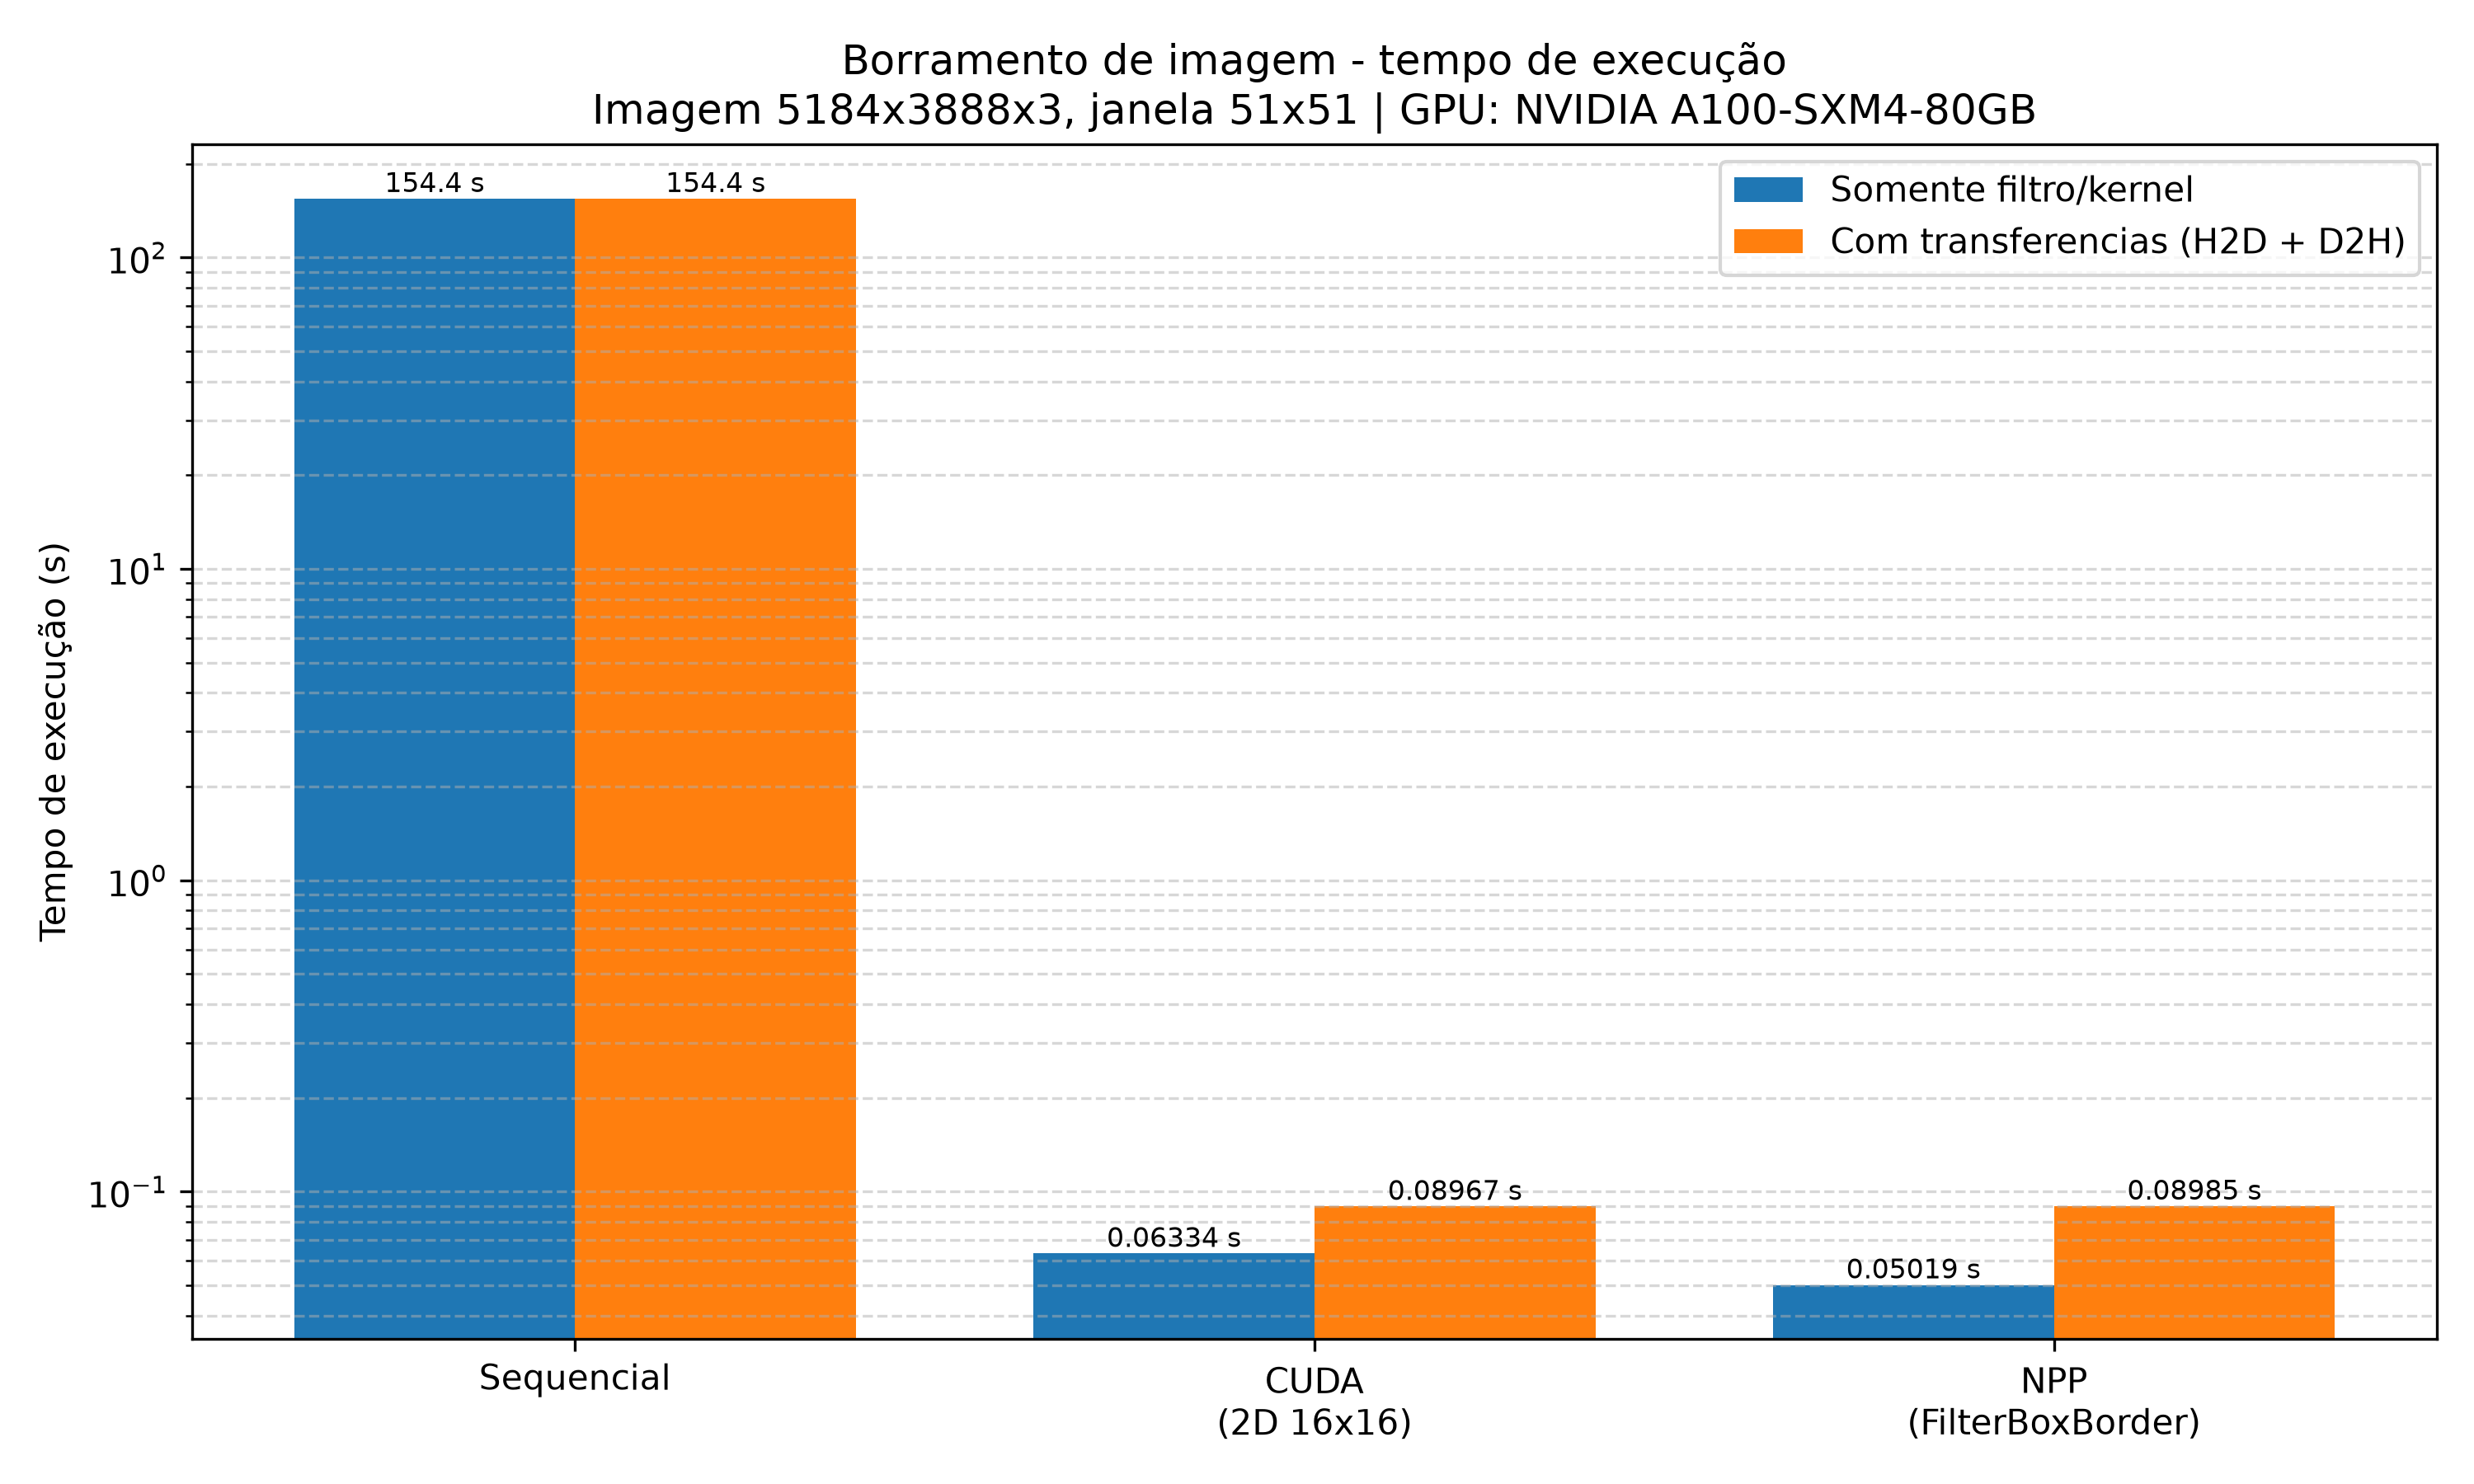
\includegraphics[width=\linewidth]{Tarefa15/tarefa15_tempos.png}
	\end{figure}
	\begin{figure}[H]
		\centering
		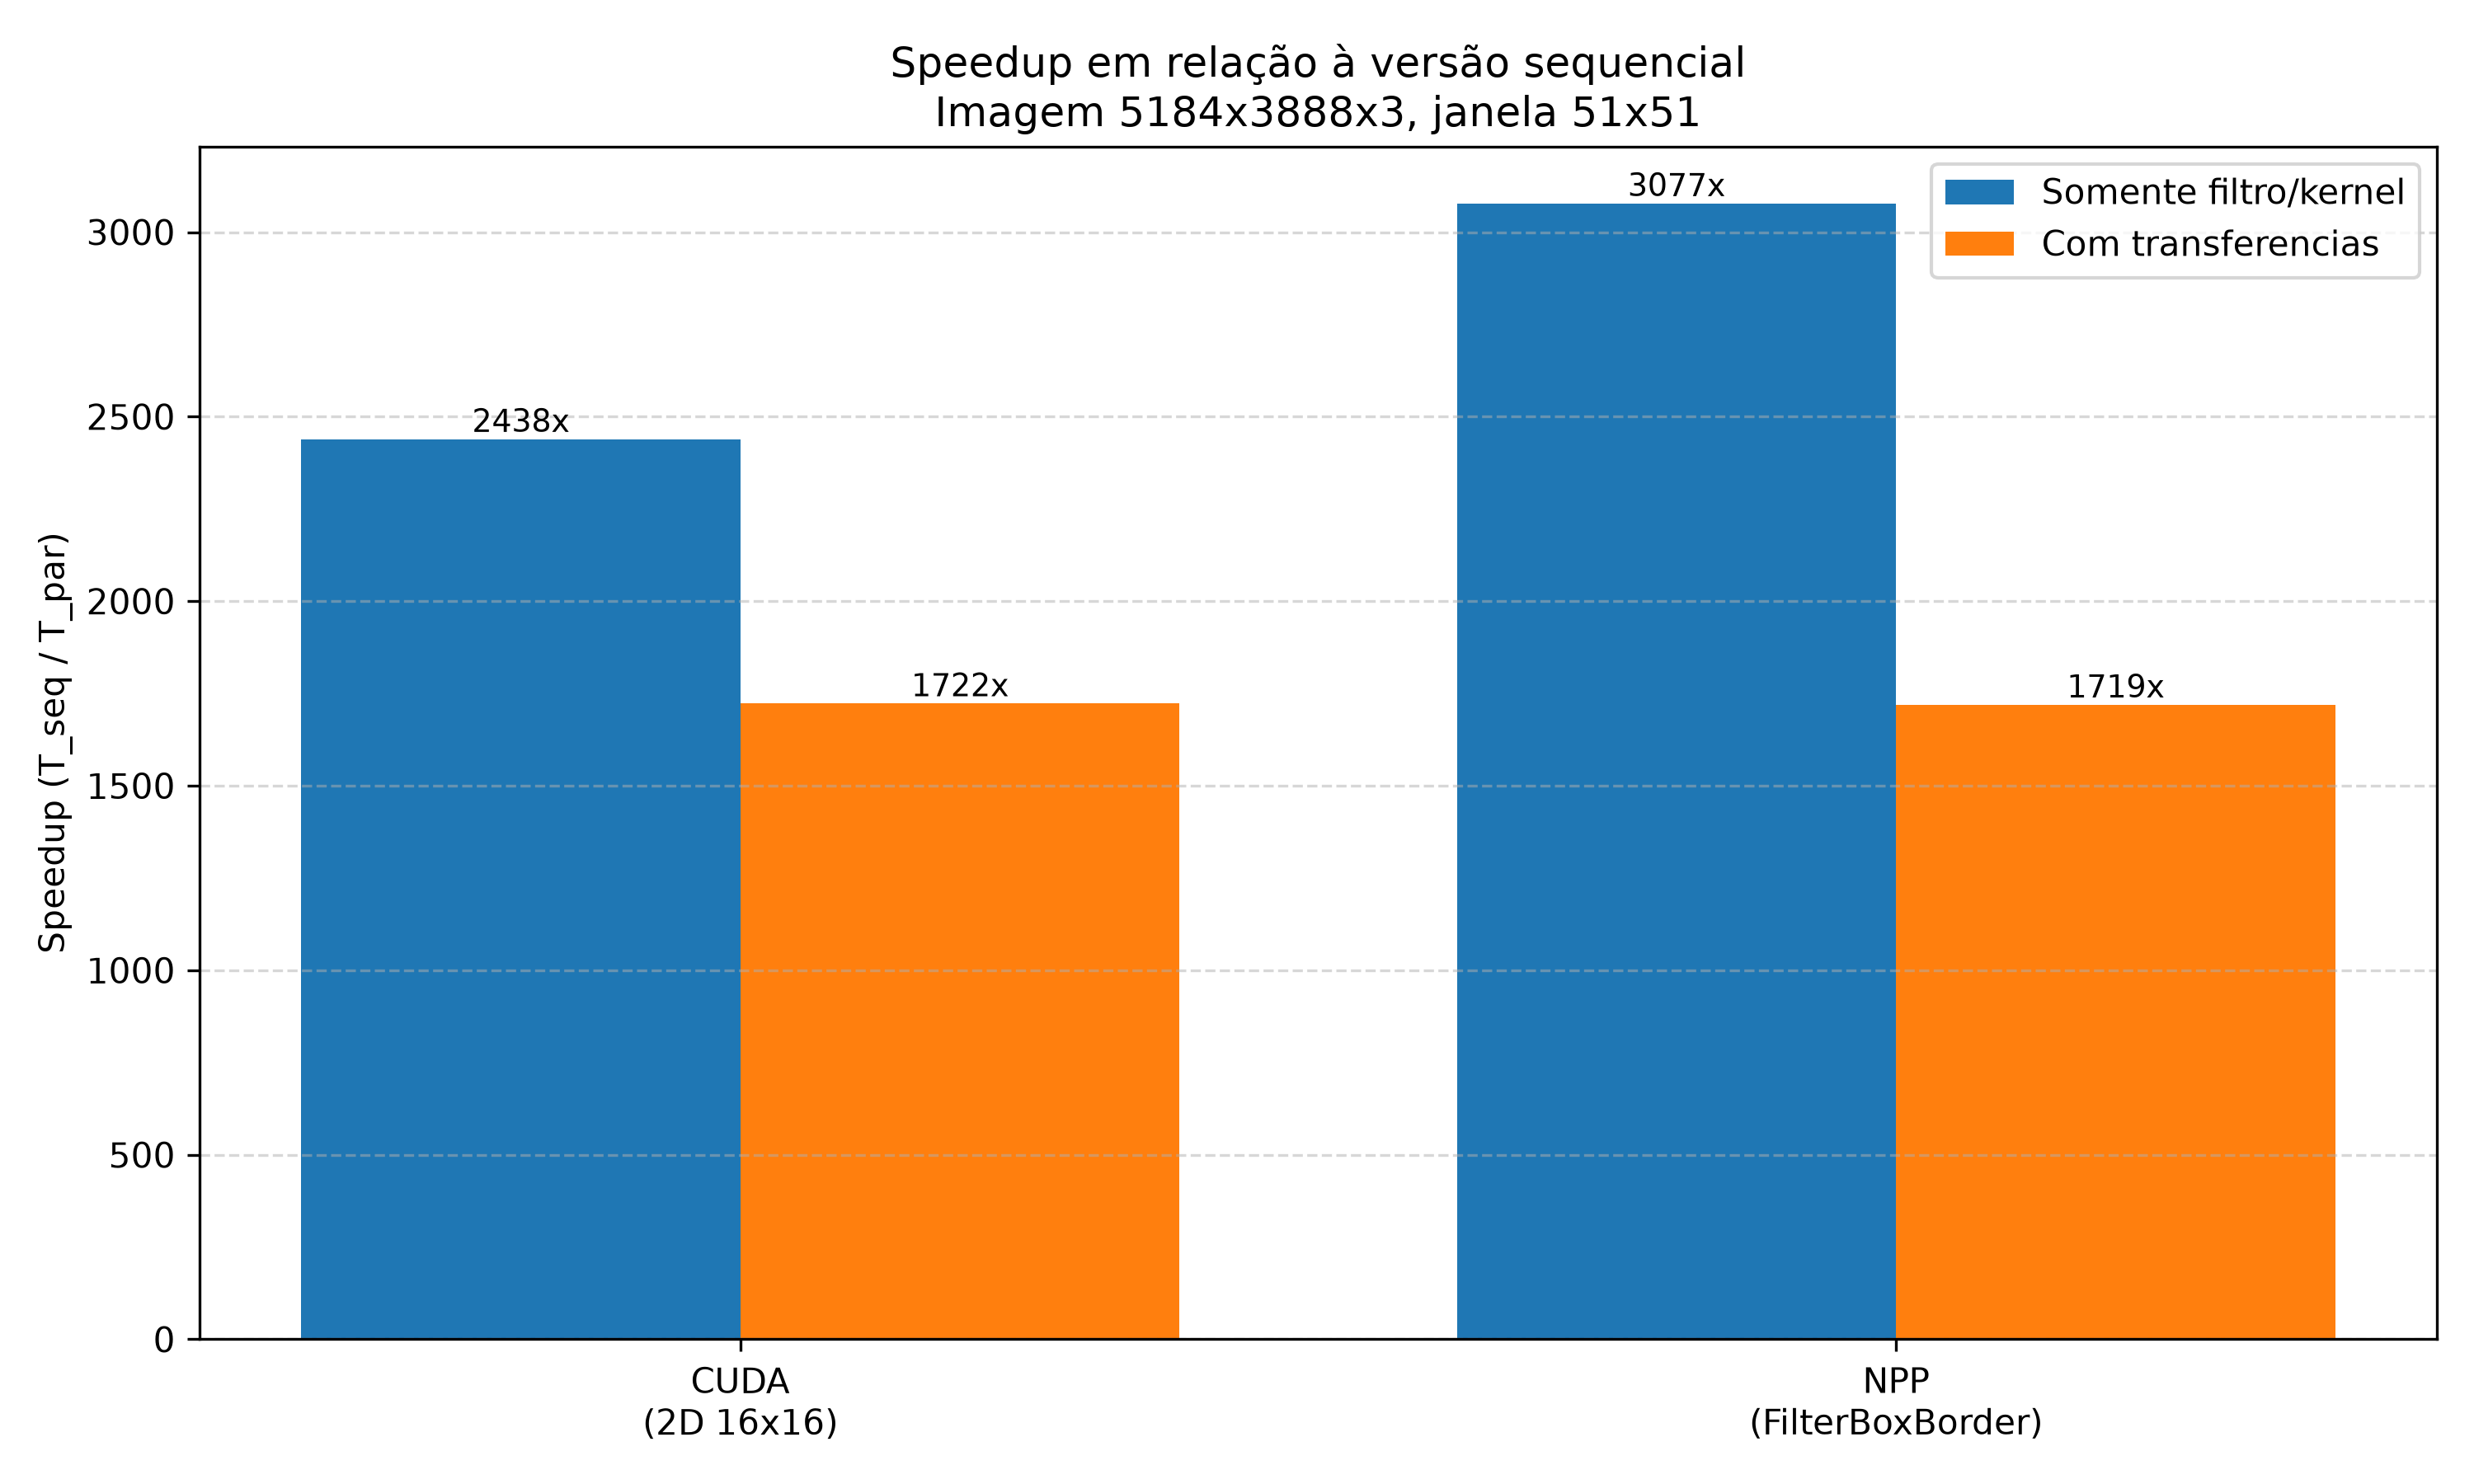
\includegraphics[width=\linewidth]{Tarefa15/tarefa15_speedup.png}
	\end{figure}
	\begin{figure}[H]
		\centering
		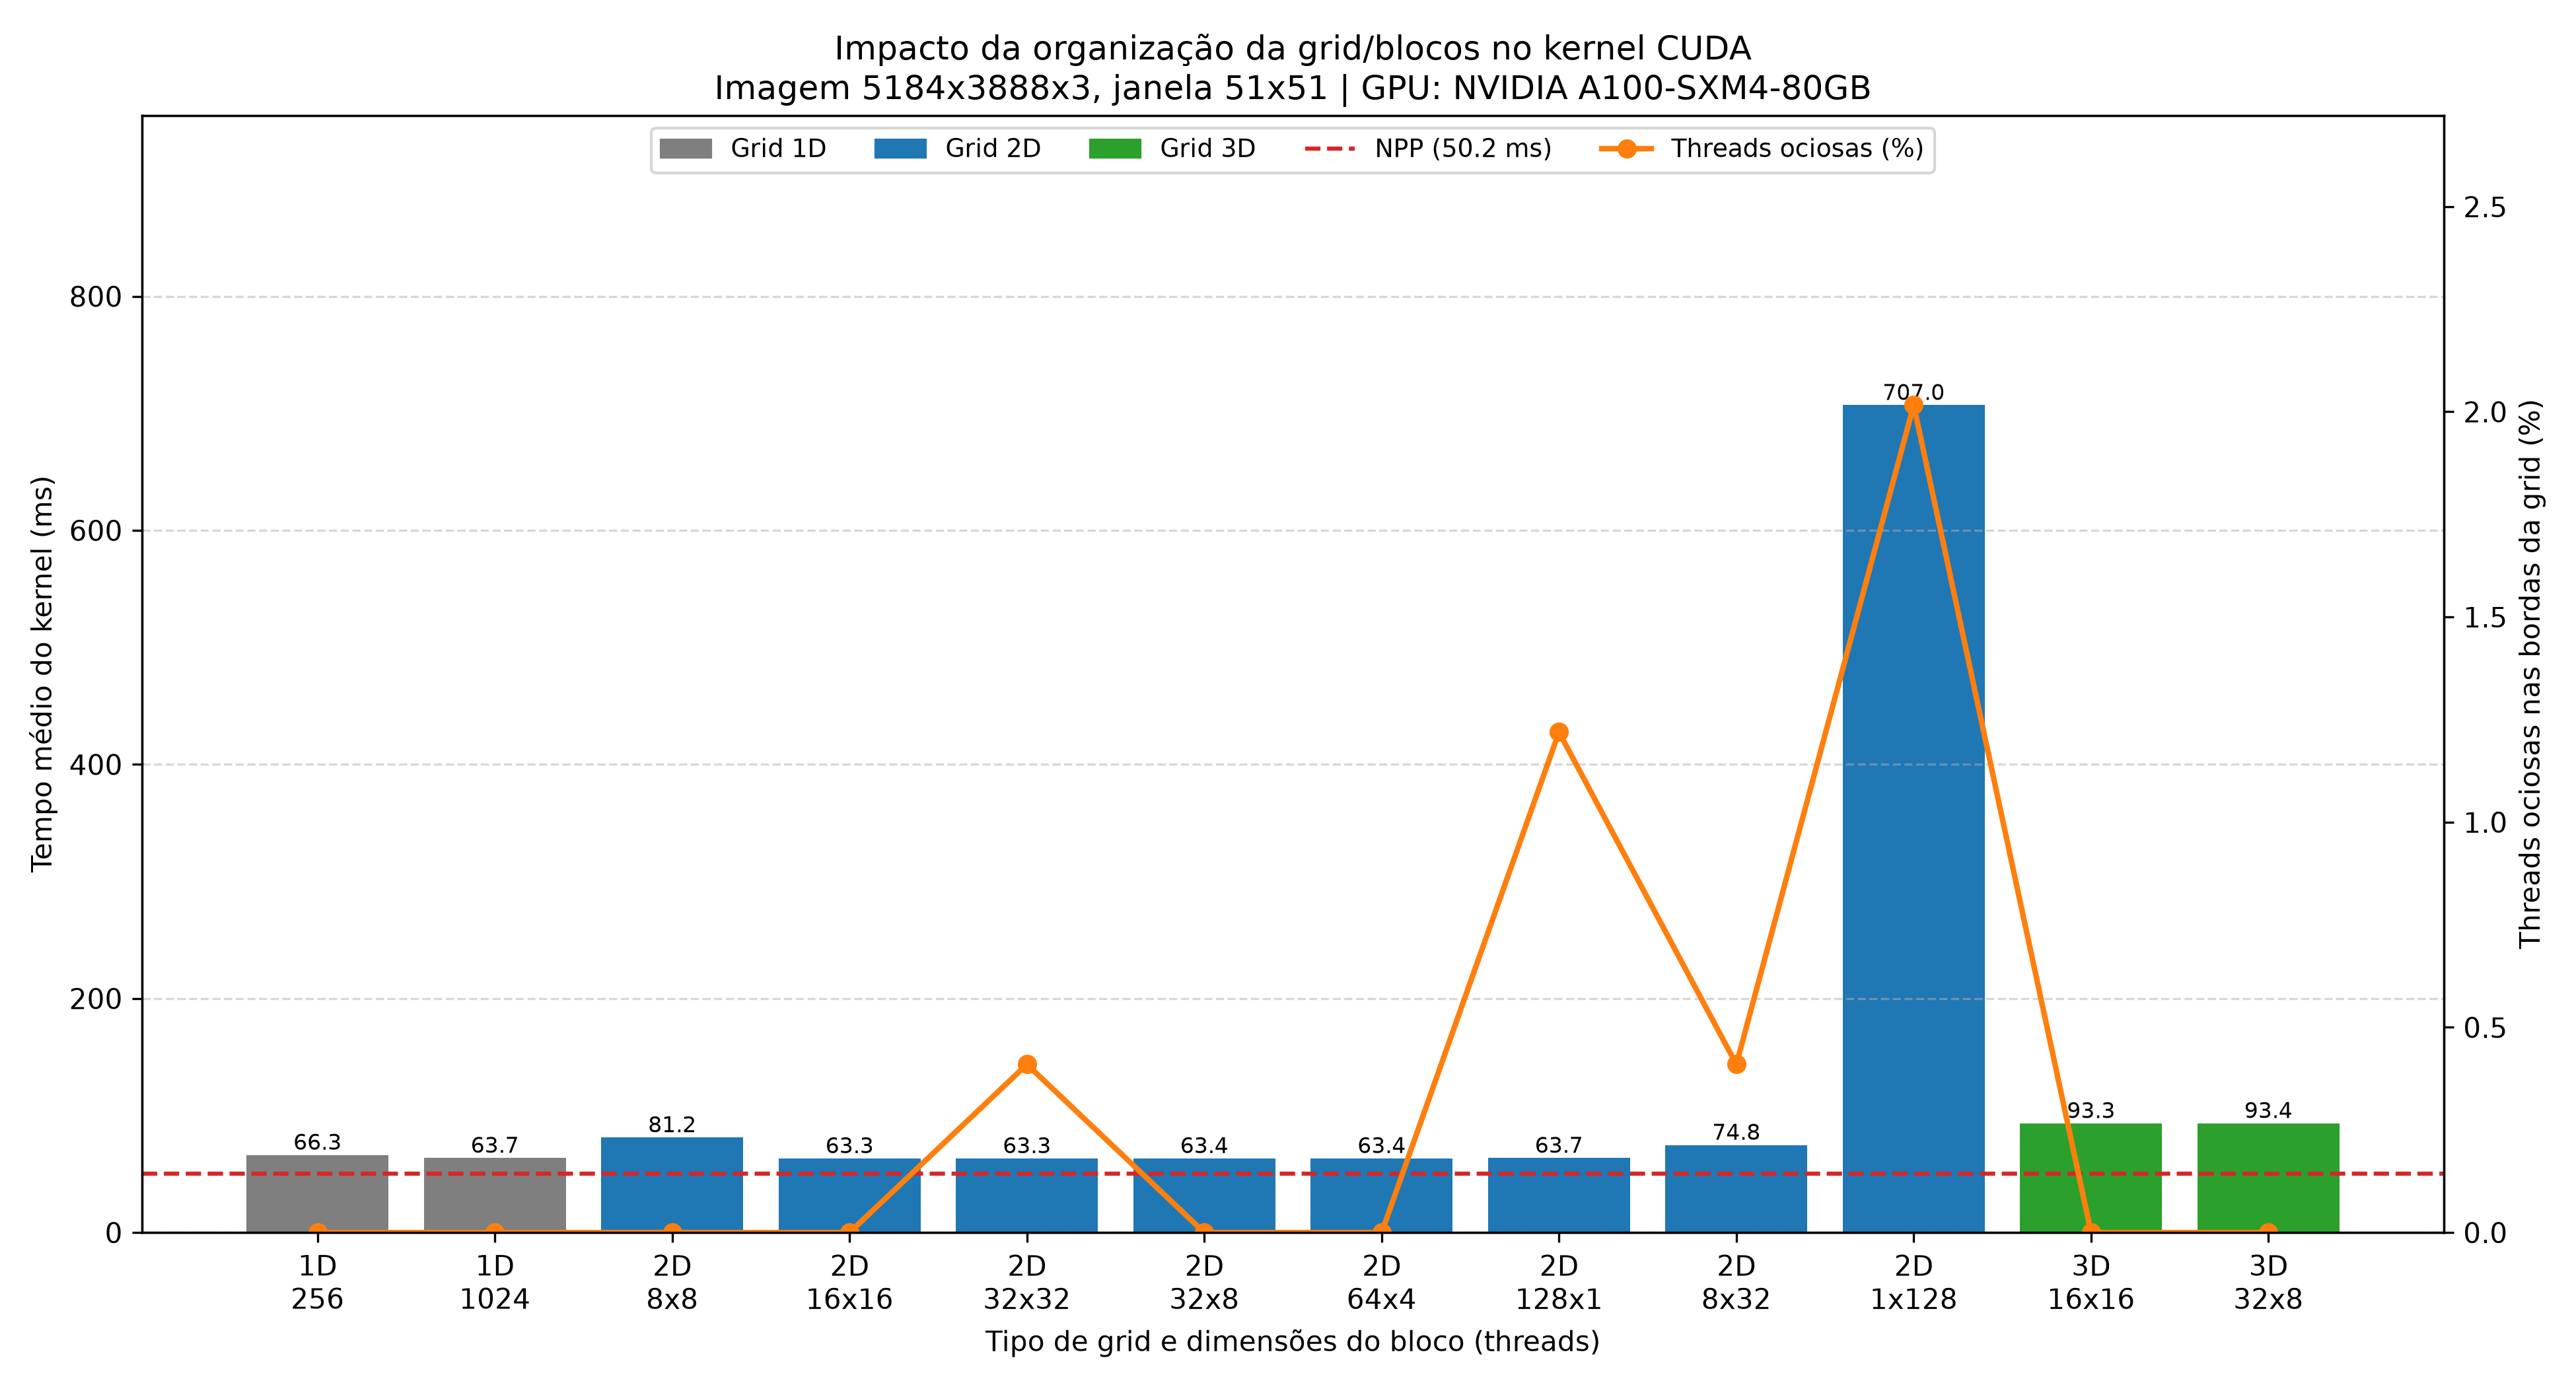
\includegraphics[width=\linewidth]{Tarefa15/tarefa15_grid.png}

	\end{figure}
	\par{
		Na versão em CUDA, cada thread calcula um pixel, usando uma grid bidimensional em que os eixos x e y das threads correspondem às colunas e linhas da imagem. Na versão com NPP, foi usada a função de filtro de média da biblioteca, com a mesma janela de 51x51. As duas versões produziram o mesmo resultado da versão sequencial.
		
		A versão sequencial levou 154,4 s, enquanto o kernel em CUDA levou 63,3 ms e o filtro do NPP 50,2 ms, mais de 2400 vezes mais rápidos. Considerando as transferências entre CPU e GPU, as duas versões paralelas ficaram com cerca de 89 ms.
		
		Adaptar a grid ao formato da imagem facilita o mapeamento das threads e permite que as threads de um warp leiam pixels vizinhos da mesma linha, por isso os blocos mais largos no eixo x tiveram os melhores tempos. Por outro lado, o formato do bloco precisa seguir a forma como a imagem está na memória: o bloco de 1x128 foi 11 vezes mais lento, e a grid 3D, com um canal de cor por thread, também foi mais lenta. Blocos que não dividem exatamente a imagem também deixam threads ociosas nas bordas, mas com impacto pequeno.
	}
	\subsection{\subtTres}
	\begin{lstlisting}[language=c, title=blur\_par.cu]
#include <stdio.h>
#include <stdlib.h>
#include <string.h>

#define STB_IMAGE_IMPLEMENTATION
#include "stb_image.h"

#define STB_IMAGE_WRITE_IMPLEMENTATION
#include "stb_image_write.h"

#define RAIO_BLUR 25
#define REPETICOES 5
#define AMOSTRAS_VERIFICACAO 2000

#define ARQUIVO_JSON "resultados_cuda.json"

#define CUDA_CHECK(chamada)                                              \
    do {                                                                 \
        cudaError_t erro_ = (chamada);                                   \
        if (erro_ != cudaSuccess) {                                      \
            fprintf(stderr, "Erro CUDA %s:%d: %s\n", __FILE__, __LINE__, \
                    cudaGetErrorString(erro_));                          \
            exit(EXIT_FAILURE);                                          \
        }                                                                \
    } while (0)

typedef enum { GRID_1D = 1, GRID_2D = 2, GRID_3D = 3 } TipoGrid;

typedef struct {
    TipoGrid tipo;
    unsigned int bx;
    unsigned int by;
} Configuracao;

static const Configuracao configuracoes[] = {
    {GRID_1D, 256, 1},
    {GRID_1D, 1024, 1},
    {GRID_2D, 8, 8},
    {GRID_2D, 16, 16},
    {GRID_2D, 32, 32},
    {GRID_2D, 32, 8},
    {GRID_2D, 64, 4},
    {GRID_2D, 128, 1},
    {GRID_2D, 8, 32},
    {GRID_2D, 1, 128},
    {GRID_3D, 16, 16},
    {GRID_3D, 32, 8},
};

static const size_t quantidade_configuracoes =
    sizeof(configuracoes) / sizeof(configuracoes[0]);

__host__ __device__ inline unsigned char media_vizinhanca(
    const unsigned char *entrada, int x, int y, int c,
    int largura, int altura, int canais)
{
    int x0 = x - RAIO_BLUR < 0 ? 0 : x - RAIO_BLUR;
    int y0 = y - RAIO_BLUR < 0 ? 0 : y - RAIO_BLUR;
    int x1 = x + RAIO_BLUR >= largura ? largura - 1 : x + RAIO_BLUR;
    int y1 = y + RAIO_BLUR >= altura ? altura - 1 : y + RAIO_BLUR;

    long soma = 0;
    for (int ny = y0; ny <= y1; ny++) {
        const unsigned char *linha = entrada + (size_t)ny * largura * canais;
        for (int nx = x0; nx <= x1; nx++) {
            soma += linha[nx * canais + c];
        }
    }

    int quantidade = (x1 - x0 + 1) * (y1 - y0 + 1);
    return (unsigned char)(soma / quantidade);
}

__global__ void blur_kernel_1d(const unsigned char *entrada,
                               unsigned char *saida,
                               int largura, int altura, int canais)
{
    size_t id = (size_t)blockIdx.x * blockDim.x + threadIdx.x;
    size_t total = (size_t)largura * altura;

    if (id >= total) return;

    int x = (int)(id % largura);
    int y = (int)(id / largura);

    for (int c = 0; c < canais; c++) {
        saida[id * canais + c] =
            media_vizinhanca(entrada, x, y, c, largura, altura, canais);
    }
}

__global__ void blur_kernel_2d(const unsigned char *entrada,
                               unsigned char *saida,
                               int largura, int altura, int canais)
{
    int x = blockIdx.x * blockDim.x + threadIdx.x;
    int y = blockIdx.y * blockDim.y + threadIdx.y;

    if (x >= largura || y >= altura) return;

    size_t indice = ((size_t)y * largura + x) * canais;

    for (int c = 0; c < canais; c++) {
        saida[indice + c] =
            media_vizinhanca(entrada, x, y, c, largura, altura, canais);
    }
}

__global__ void blur_kernel_3d(const unsigned char *entrada,
                               unsigned char *saida,
                               int largura, int altura, int canais)
{
    int x = blockIdx.x * blockDim.x + threadIdx.x;
    int y = blockIdx.y * blockDim.y + threadIdx.y;
    int c = blockIdx.z;

    if (x >= largura || y >= altura || c >= canais) return;

    size_t indice = ((size_t)y * largura + x) * canais + c;

    saida[indice] =
        media_vizinhanca(entrada, x, y, c, largura, altura, canais);
}

static void monta_grid(const Configuracao *cfg, int largura, int altura,
                       int canais, dim3 *grid, dim3 *bloco)
{
    if (cfg->tipo == GRID_1D) {
        size_t total = (size_t)largura * altura;
        *bloco = dim3(cfg->bx, 1, 1);
        *grid = dim3((unsigned int)((total + cfg->bx - 1) / cfg->bx), 1, 1);
    } else {
        *bloco = dim3(cfg->bx, cfg->by, 1);
        *grid = dim3((largura + cfg->bx - 1) / cfg->bx,
                     (altura + cfg->by - 1) / cfg->by,
                     cfg->tipo == GRID_3D ? canais : 1);
    }
}

static void lanca_kernel(const Configuracao *cfg, dim3 grid, dim3 bloco,
                         const unsigned char *d_entrada,
                         unsigned char *d_saida,
                         int largura, int altura, int canais)
{
    switch (cfg->tipo) {
    case GRID_1D:
        blur_kernel_1d<<<grid, bloco>>>(d_entrada, d_saida,
                                        largura, altura, canais);
        break;
    case GRID_2D:
        blur_kernel_2d<<<grid, bloco>>>(d_entrada, d_saida,
                                        largura, altura, canais);
        break;
    case GRID_3D:
        blur_kernel_3d<<<grid, bloco>>>(d_entrada, d_saida,
                                        largura, altura, canais);
        break;
    }
}

static int verifica_amostras(const unsigned char *entrada,
                             const unsigned char *saida_gpu,
                             int largura, int altura, int canais)
{
    int erros = 0;
    srand(42);
    for (int i = 0; i < AMOSTRAS_VERIFICACAO; i++) {
        int x = rand() % largura;
        int y = rand() % altura;
        for (int c = 0; c < canais; c++) {
            unsigned char ref =
                media_vizinhanca(entrada, x, y, c, largura, altura, canais);
            size_t indice = ((size_t)y * largura + x) * canais + c;
            if (ref != saida_gpu[indice]) erros++;
        }
    }
    return erros;
}

static const char *nome_tipo(TipoGrid tipo)
{
    switch (tipo) {
    case GRID_1D: return "1D";
    case GRID_2D: return "2D";
    case GRID_3D: return "3D";
    }
    return "?";
}

int main(int argc, char *argv[])
{
    if (argc != 3) {
        printf("Uso: %s entrada.jpg saida.jpg\n", argv[0]);
        return 1;
    }

    int largura, altura, canais;

    unsigned char *imagem = stbi_load(argv[1], &largura, &altura, &canais, 0);

    if (imagem == NULL) {
        fprintf(stderr, "Erro ao ler imagem: %s\n", stbi_failure_reason());
        return 1;
    }

    size_t tamanho = (size_t)largura * altura * canais;

    unsigned char *resultado = (unsigned char *)malloc(tamanho);

    if (resultado == NULL) {
        fprintf(stderr, "Erro ao alocar memoria.\n");
        stbi_image_free(imagem);
        return 1;
    }

    cudaDeviceProp prop;
    CUDA_CHECK(cudaGetDeviceProperties(&prop, 0));

    printf("GPU: %s (SMs: %d)\n", prop.name, prop.multiProcessorCount);
    printf("Imagem: %d x %d, canais: %d\n", largura, altura, canais);
    printf("Aplicando blur com janela %dx%d...\n",
           2 * RAIO_BLUR + 1, 2 * RAIO_BLUR + 1);

    unsigned char *d_entrada = NULL;
    unsigned char *d_saida = NULL;

    CUDA_CHECK(cudaMalloc(&d_entrada, tamanho));
    CUDA_CHECK(cudaMalloc(&d_saida, tamanho));

    cudaEvent_t ini, fim;
    CUDA_CHECK(cudaEventCreate(&ini));
    CUDA_CHECK(cudaEventCreate(&fim));

    float tempo_h2d_ms = 0.0f;
    CUDA_CHECK(cudaEventRecord(ini));
    CUDA_CHECK(cudaMemcpy(d_entrada, imagem, tamanho, cudaMemcpyHostToDevice));
    CUDA_CHECK(cudaEventRecord(fim));
    CUDA_CHECK(cudaEventSynchronize(fim));
    CUDA_CHECK(cudaEventElapsedTime(&tempo_h2d_ms, ini, fim));

    {
        dim3 grid, bloco;
        Configuracao aquecimento = {GRID_2D, 16, 16};
        monta_grid(&aquecimento, largura, altura, canais, &grid, &bloco);
        lanca_kernel(&aquecimento, grid, bloco, d_entrada, d_saida,
                     largura, altura, canais);
        CUDA_CHECK(cudaGetLastError());
        CUDA_CHECK(cudaDeviceSynchronize());
    }

    FILE *json = fopen(ARQUIVO_JSON, "w");
    if (json == NULL) {
        fprintf(stderr, "Erro ao abrir %s\n", ARQUIVO_JSON);
        return 1;
    }

    fprintf(json, "{\n");
    fprintf(json, "  \"versao\": \"cuda\",\n");
    fprintf(json, "  \"gpu\": \"%s\",\n", prop.name);
    fprintf(json, "  \"largura\": %d,\n", largura);
    fprintf(json, "  \"altura\": %d,\n", altura);
    fprintf(json, "  \"canais\": %d,\n", canais);
    fprintf(json, "  \"raio\": %d,\n", RAIO_BLUR);
    fprintf(json, "  \"repeticoes\": %d,\n", REPETICOES);
    fprintf(json, "  \"tempo_h2d_ms\": %f,\n", tempo_h2d_ms);

    float tempo_d2h_ms = 0.0f;
    float melhor_kernel_ms = 1e30f;

    fprintf(json, "  \"configuracoes\": [\n");

    for (size_t i = 0; i < quantidade_configuracoes; i++) {
        const Configuracao *cfg = &configuracoes[i];

        dim3 grid, bloco;
        monta_grid(cfg, largura, altura, canais, &grid, &bloco);

        CUDA_CHECK(cudaMemset(d_saida, 0, tamanho));

        float soma_ms = 0.0f, min_ms = 1e30f, max_ms = 0.0f;

        for (int r = 0; r < REPETICOES; r++) {
            float ms = 0.0f;
            CUDA_CHECK(cudaEventRecord(ini));
            lanca_kernel(cfg, grid, bloco, d_entrada, d_saida,
                         largura, altura, canais);
            CUDA_CHECK(cudaEventRecord(fim));
            CUDA_CHECK(cudaEventSynchronize(fim));
            CUDA_CHECK(cudaGetLastError());
            CUDA_CHECK(cudaEventElapsedTime(&ms, ini, fim));
            soma_ms += ms;
            if (ms < min_ms) min_ms = ms;
            if (ms > max_ms) max_ms = ms;
        }

        float media_ms = soma_ms / REPETICOES;

        float ms_d2h = 0.0f;
        CUDA_CHECK(cudaEventRecord(ini));
        CUDA_CHECK(cudaMemcpy(resultado, d_saida, tamanho,
                              cudaMemcpyDeviceToHost));
        CUDA_CHECK(cudaEventRecord(fim));
        CUDA_CHECK(cudaEventSynchronize(fim));
        CUDA_CHECK(cudaEventElapsedTime(&ms_d2h, ini, fim));
        tempo_d2h_ms = ms_d2h;

        int erros = verifica_amostras(imagem, resultado,
                                      largura, altura, canais);

        unsigned long long threads_lancadas =
            (unsigned long long)grid.x * grid.y * grid.z *
            bloco.x * bloco.y * bloco.z;
        unsigned long long threads_uteis =
            (unsigned long long)largura * altura *
            (cfg->tipo == GRID_3D ? canais : 1);
        double ociosas_pct =
            100.0 * (double)(threads_lancadas - threads_uteis) /
            (double)threads_lancadas;

        double tempo_total_ms = tempo_h2d_ms + media_ms + ms_d2h;

        printf("[CUDA %s] bloco (%3u,%3u,%u) grid (%5u,%5u,%u) | "
               "kernel: %9.3f ms (min %9.3f) | total: %9.3f ms | "
               "ociosas: %5.2f%% | erros: %d\n",
               nome_tipo(cfg->tipo), bloco.x, bloco.y, bloco.z,
               grid.x, grid.y, grid.z, media_ms, min_ms, tempo_total_ms,
               ociosas_pct, erros);

        fprintf(json,
                "    {\"tipo\": \"%s\", \"bloco\": [%u, %u, %u], "
                "\"grid\": [%u, %u, %u], "
                "\"threads_por_bloco\": %u, "
                "\"threads_lancadas\": %llu, "
                "\"threads_ociosas_pct\": %f, "
                "\"tempo_kernel_ms\": %f, \"tempo_kernel_min_ms\": %f, "
                "\"tempo_kernel_max_ms\": %f, \"tempo_d2h_ms\": %f, "
                "\"tempo_total_ms\": %f, \"erros_verificacao\": %d}%s\n",
                nome_tipo(cfg->tipo), bloco.x, bloco.y, bloco.z,
                grid.x, grid.y, grid.z, bloco.x * bloco.y * bloco.z,
                threads_lancadas, ociosas_pct, media_ms, min_ms, max_ms,
                ms_d2h, tempo_total_ms, erros,
                i + 1 < quantidade_configuracoes ? "," : "");

        if (media_ms < melhor_kernel_ms) melhor_kernel_ms = media_ms;
    }

    fprintf(json, "  ],\n");
    fprintf(json, "  \"tempo_d2h_ms\": %f,\n", tempo_d2h_ms);
    fprintf(json, "  \"melhor_tempo_kernel_ms\": %f\n", melhor_kernel_ms);
    fprintf(json, "}\n");
    fclose(json);

    printf("Resultados salvos em %s\n", ARQUIVO_JSON);

    {
        dim3 grid, bloco;
        Configuracao cfg = {GRID_2D, 16, 16};
        monta_grid(&cfg, largura, altura, canais, &grid, &bloco);
        lanca_kernel(&cfg, grid, bloco, d_entrada, d_saida,
                     largura, altura, canais);
        CUDA_CHECK(cudaDeviceSynchronize());
        CUDA_CHECK(cudaMemcpy(resultado, d_saida, tamanho,
                              cudaMemcpyDeviceToHost));
    }

    int sucesso = stbi_write_jpg(argv[2], largura, altura, canais,
                                 resultado, 95);

    if (!sucesso) {
        fprintf(stderr, "Erro ao salvar imagem.\n");
    } else {
        printf("Imagem borrada salva em: %s\n", argv[2]);
    }

    CUDA_CHECK(cudaEventDestroy(ini));
    CUDA_CHECK(cudaEventDestroy(fim));
    CUDA_CHECK(cudaFree(d_entrada));
    CUDA_CHECK(cudaFree(d_saida));
    stbi_image_free(imagem);
    free(resultado);

    return sucesso ? 0 : 1;
}
\end{lstlisting}
	\begin{lstlisting}[language=c, title=blur\_npp.cu]
#include <stdio.h>
#include <stdlib.h>
#include <string.h>

#include <cuda_runtime.h>
#include <npp.h>

#define STB_IMAGE_IMPLEMENTATION
#include "stb_image.h"

#define STB_IMAGE_WRITE_IMPLEMENTATION
#include "stb_image_write.h"

#define RAIO_BLUR 25
#define REPETICOES 5
#define AMOSTRAS_VERIFICACAO 2000
#define TOLERANCIA 1

#define ARQUIVO_JSON "resultados_npp.json"

#define CUDA_CHECK(chamada)                                              \
    do {                                                                 \
        cudaError_t erro_ = (chamada);                                   \
        if (erro_ != cudaSuccess) {                                      \
            fprintf(stderr, "Erro CUDA %s:%d: %s\n", __FILE__, __LINE__, \
                    cudaGetErrorString(erro_));                          \
            exit(EXIT_FAILURE);                                          \
        }                                                                \
    } while (0)

#define NPP_CHECK(chamada)                                               \
    do {                                                                 \
        NppStatus status_ = (chamada);                                   \
        if (status_ != NPP_SUCCESS) {                                    \
            fprintf(stderr, "Erro NPP %s:%d: codigo %d\n", __FILE__,     \
                    __LINE__, (int)status_);                             \
            exit(EXIT_FAILURE);                                          \
        }                                                                \
    } while (0)

static NppStreamContext cria_contexto_npp(cudaStream_t stream)
{
    NppStreamContext ctx;
    memset(&ctx, 0, sizeof(ctx));

    int dispositivo = 0;
    CUDA_CHECK(cudaGetDevice(&dispositivo));

    cudaDeviceProp prop;
    CUDA_CHECK(cudaGetDeviceProperties(&prop, dispositivo));

    ctx.hStream = stream;
    ctx.nCudaDeviceId = dispositivo;
    ctx.nMultiProcessorCount = prop.multiProcessorCount;
    ctx.nMaxThreadsPerMultiProcessor = prop.maxThreadsPerMultiProcessor;
    ctx.nMaxThreadsPerBlock = prop.maxThreadsPerBlock;
    ctx.nSharedMemPerBlock = prop.sharedMemPerBlock;
    CUDA_CHECK(cudaDeviceGetAttribute(&ctx.nCudaDevAttrComputeCapabilityMajor,
                                      cudaDevAttrComputeCapabilityMajor,
                                      dispositivo));
    CUDA_CHECK(cudaDeviceGetAttribute(&ctx.nCudaDevAttrComputeCapabilityMinor,
                                      cudaDevAttrComputeCapabilityMinor,
                                      dispositivo));
    CUDA_CHECK(cudaStreamGetFlags(stream, &ctx.nStreamFlags));

    return ctx;
}

static void filtro_npp(const Npp8u *d_entrada, int passo_entrada,
                       Npp8u *d_saida, int passo_saida,
                       int largura, int altura, int canais,
                       NppStreamContext ctx)
{
    NppiSize tamanho_img = {largura, altura};
    NppiPoint deslocamento = {0, 0};
    NppiSize mascara = {2 * RAIO_BLUR + 1, 2 * RAIO_BLUR + 1};
    NppiPoint ancora = {RAIO_BLUR, RAIO_BLUR};

    switch (canais) {
    case 1:
        NPP_CHECK(nppiFilterBoxBorder_8u_C1R_Ctx(
            d_entrada, passo_entrada, tamanho_img, deslocamento,
            d_saida, passo_saida, tamanho_img, mascara, ancora,
            NPP_BORDER_REPLICATE, ctx));
        break;
    case 3:
        NPP_CHECK(nppiFilterBoxBorder_8u_C3R_Ctx(
            d_entrada, passo_entrada, tamanho_img, deslocamento,
            d_saida, passo_saida, tamanho_img, mascara, ancora,
            NPP_BORDER_REPLICATE, ctx));
        break;
    case 4:
        NPP_CHECK(nppiFilterBoxBorder_8u_C4R_Ctx(
            d_entrada, passo_entrada, tamanho_img, deslocamento,
            d_saida, passo_saida, tamanho_img, mascara, ancora,
            NPP_BORDER_REPLICATE, ctx));
        break;
    default:
        fprintf(stderr, "Numero de canais nao suportado: %d\n", canais);
        exit(EXIT_FAILURE);
    }
}

static int media_referencia(const unsigned char *entrada, int x, int y, int c,
                            int largura, int altura, int canais)
{
    long soma = 0;
    int quantidade = 0;
    for (int dy = -RAIO_BLUR; dy <= RAIO_BLUR; dy++) {
        for (int dx = -RAIO_BLUR; dx <= RAIO_BLUR; dx++) {
            int nx = x + dx, ny = y + dy;
            if (nx >= 0 && nx < largura && ny >= 0 && ny < altura) {
                soma += entrada[((size_t)ny * largura + nx) * canais + c];
                quantidade++;
            }
        }
    }
    return (int)(soma / quantidade);
}

static int verifica_amostras(const unsigned char *entrada,
                             const unsigned char *saida,
                             int largura, int altura, int canais,
                             int *maior_diferenca)
{
    int erros = 0;
    *maior_diferenca = 0;
    srand(42);
    for (int i = 0; i < AMOSTRAS_VERIFICACAO; i++) {
        int x = RAIO_BLUR + rand() % (largura - 2 * RAIO_BLUR);
        int y = RAIO_BLUR + rand() % (altura - 2 * RAIO_BLUR);
        for (int c = 0; c < canais; c++) {
            int ref = media_referencia(entrada, x, y, c,
                                       largura, altura, canais);
            int val = saida[((size_t)y * largura + x) * canais + c];
            int dif = abs(ref - val);
            if (dif > *maior_diferenca) *maior_diferenca = dif;
            if (dif > TOLERANCIA) erros++;
        }
    }
    return erros;
}

int main(int argc, char *argv[])
{
    if (argc != 3) {
        printf("Uso: %s entrada.jpg saida.jpg\n", argv[0]);
        return 1;
    }

    int largura, altura, canais;

    unsigned char *imagem = stbi_load(argv[1], &largura, &altura, &canais, 0);

    if (imagem == NULL) {
        fprintf(stderr, "Erro ao ler imagem: %s\n", stbi_failure_reason());
        return 1;
    }

    size_t passo_host = (size_t)largura * canais;
    size_t tamanho = passo_host * altura;

    unsigned char *resultado = (unsigned char *)malloc(tamanho);

    if (resultado == NULL) {
        fprintf(stderr, "Erro ao alocar memoria.\n");
        stbi_image_free(imagem);
        return 1;
    }

    cudaDeviceProp prop;
    CUDA_CHECK(cudaGetDeviceProperties(&prop, 0));

    const NppLibraryVersion *versao = nppGetLibVersion();

    printf("GPU: %s | NPP %d.%d.%d\n", prop.name,
           versao->major, versao->minor, versao->build);
    printf("Imagem: %d x %d, canais: %d\n", largura, altura, canais);
    printf("Aplicando box filter NPP com mascara %dx%d...\n",
           2 * RAIO_BLUR + 1, 2 * RAIO_BLUR + 1);

    Npp8u *d_entrada = NULL, *d_saida = NULL;
    size_t passo_entrada = 0, passo_saida = 0;

    CUDA_CHECK(cudaMallocPitch((void **)&d_entrada, &passo_entrada,
                               passo_host, altura));
    CUDA_CHECK(cudaMallocPitch((void **)&d_saida, &passo_saida,
                               passo_host, altura));

    cudaStream_t stream;
    CUDA_CHECK(cudaStreamCreate(&stream));
    NppStreamContext ctx = cria_contexto_npp(stream);

    cudaEvent_t ini, fim;
    CUDA_CHECK(cudaEventCreate(&ini));
    CUDA_CHECK(cudaEventCreate(&fim));

    float tempo_h2d_ms = 0.0f;
    CUDA_CHECK(cudaEventRecord(ini, stream));
    CUDA_CHECK(cudaMemcpy2DAsync(d_entrada, passo_entrada, imagem, passo_host,
                                 passo_host, altura, cudaMemcpyHostToDevice,
                                 stream));
    CUDA_CHECK(cudaEventRecord(fim, stream));
    CUDA_CHECK(cudaEventSynchronize(fim));
    CUDA_CHECK(cudaEventElapsedTime(&tempo_h2d_ms, ini, fim));

    filtro_npp(d_entrada, (int)passo_entrada, d_saida, (int)passo_saida,
               largura, altura, canais, ctx);
    CUDA_CHECK(cudaStreamSynchronize(stream));

    float soma_ms = 0.0f, min_ms = 1e30f, max_ms = 0.0f;

    for (int r = 0; r < REPETICOES; r++) {
        float ms = 0.0f;
        CUDA_CHECK(cudaEventRecord(ini, stream));
        filtro_npp(d_entrada, (int)passo_entrada, d_saida, (int)passo_saida,
                   largura, altura, canais, ctx);
        CUDA_CHECK(cudaEventRecord(fim, stream));
        CUDA_CHECK(cudaEventSynchronize(fim));
        CUDA_CHECK(cudaEventElapsedTime(&ms, ini, fim));
        soma_ms += ms;
        if (ms < min_ms) min_ms = ms;
        if (ms > max_ms) max_ms = ms;
    }

    float media_ms = soma_ms / REPETICOES;

    float tempo_d2h_ms = 0.0f;
    CUDA_CHECK(cudaEventRecord(ini, stream));
    CUDA_CHECK(cudaMemcpy2DAsync(resultado, passo_host, d_saida, passo_saida,
                                 passo_host, altura, cudaMemcpyDeviceToHost,
                                 stream));
    CUDA_CHECK(cudaEventRecord(fim, stream));
    CUDA_CHECK(cudaEventSynchronize(fim));
    CUDA_CHECK(cudaEventElapsedTime(&tempo_d2h_ms, ini, fim));

    double tempo_total_ms = tempo_h2d_ms + media_ms + tempo_d2h_ms;

    int maior_diferenca = 0;
    int erros = verifica_amostras(imagem, resultado, largura, altura, canais,
                                  &maior_diferenca);

    printf("[NPP] filtro: %9.3f ms (min %9.3f) | H2D: %.3f ms | "
           "D2H: %.3f ms | total: %9.3f ms\n",
           media_ms, min_ms, tempo_h2d_ms, tempo_d2h_ms, tempo_total_ms);
    printf("[NPP] verificacao (pixels internos): %d erros, maior diferenca %d\n",
           erros, maior_diferenca);

    FILE *json = fopen(ARQUIVO_JSON, "w");
    if (json != NULL) {
        fprintf(json,
                "{\n"
                "  \"versao\": \"npp\",\n"
                "  \"gpu\": \"%s\",\n"
                "  \"npp_versao\": \"%d.%d.%d\",\n"
                "  \"funcao\": \"nppiFilterBoxBorder_8u_C%dR_Ctx\",\n"
                "  \"borda\": \"NPP_BORDER_REPLICATE\",\n"
                "  \"largura\": %d,\n"
                "  \"altura\": %d,\n"
                "  \"canais\": %d,\n"
                "  \"raio\": %d,\n"
                "  \"repeticoes\": %d,\n"
                "  \"tempo_h2d_ms\": %f,\n"
                "  \"tempo_kernel_ms\": %f,\n"
                "  \"tempo_kernel_min_ms\": %f,\n"
                "  \"tempo_kernel_max_ms\": %f,\n"
                "  \"tempo_d2h_ms\": %f,\n"
                "  \"tempo_total_ms\": %f,\n"
                "  \"erros_verificacao\": %d,\n"
                "  \"maior_diferenca\": %d\n"
                "}\n",
                prop.name, versao->major, versao->minor, versao->build,
                canais, largura, altura, canais, RAIO_BLUR, REPETICOES,
                tempo_h2d_ms, media_ms, min_ms, max_ms, tempo_d2h_ms,
                tempo_total_ms, erros, maior_diferenca);
        fclose(json);
        printf("Resultados salvos em %s\n", ARQUIVO_JSON);
    } else {
        fprintf(stderr, "Erro ao abrir %s\n", ARQUIVO_JSON);
    }

    int sucesso = stbi_write_jpg(argv[2], largura, altura, canais,
                                 resultado, 95);

    if (!sucesso) {
        fprintf(stderr, "Erro ao salvar imagem.\n");
    } else {
        printf("Imagem borrada salva em: %s\n", argv[2]);
    }

    CUDA_CHECK(cudaEventDestroy(ini));
    CUDA_CHECK(cudaEventDestroy(fim));
    CUDA_CHECK(cudaStreamDestroy(stream));
    CUDA_CHECK(cudaFree(d_entrada));
    CUDA_CHECK(cudaFree(d_saida));
    stbi_image_free(imagem);
    free(resultado);

    return sucesso ? 0 : 1;
}
\end{lstlisting}
	\begin{lstlisting}[language=bash, title=script\_cuda.sh]
#!/bin/bash
#SBATCH --job-name=CUDA_blur_akira
#SBATCH --output=saida%j.out
#SBATCH --error=erro%j.err
#SBATCH --partition=gpu-4-a100
#SBATCH --nodes=1
#SBATCH --ntasks=1
#SBATCH --cpus-per-task=1
#SBATCH --gpus-per-node=1
#SBATCH --time=0-0:30

cd "${SLURM_SUBMIT_DIR:-.}"

carrega_cuda() {
    command -v nvcc > /dev/null 2>&1 && return 0
    if ! type module > /dev/null 2>&1; then
        for f in /etc/profile.d/modules.sh /etc/profile.d/lmod.sh /usr/share/lmod/lmod/init/bash; do
            [ -f "$f" ] && source "$f" && break
        done
    fi
    if type module > /dev/null 2>&1; then
        if [ -n "$CUDA_MODULE" ]; then
            module load "$CUDA_MODULE"
        else
            for padrao in 'cuda' 'nvhpc' 'nvidia'; do
                mod=$(module -t avail 2>&1 | grep -v ':$' | grep -vE '^(containers|softwares)/' | grep -i "$padrao" | sort -V | tail -n 1)
                if [ -n "$mod" ]; then
                    echo "Carregando modulo: $mod"
                    module load "$mod" && command -v nvcc > /dev/null 2>&1 && return 0
                fi
            done
        fi
    fi
    command -v nvcc > /dev/null 2>&1 && return 0
    for d in /usr/local/cuda/bin /usr/local/cuda-*/bin /opt/cuda/bin \
             /opt/nvidia/hpc_sdk/Linux_x86_64/*/compilers/bin \
             /opt/nvidia/hpc_sdk/Linux_x86_64/*/cuda/*/bin; do
        if [ -x "$d/nvcc" ]; then
            export PATH="$d:$PATH"
            return 0
        fi
    done
    return 1
}

if ! carrega_cuda; then
    echo "nvcc nao encontrado. Modulos disponiveis:" >&2
    module -t avail 2>&1 | grep -iE 'cuda|nvhpc|nvidia' >&2
    echo "Informe o modulo: sbatch --export=ALL,CUDA_MODULE=<nome> script_cuda.sh" >&2
    exit 1
fi

echo "===== Ambiente ====="
hostname
nvidia-smi --query-gpu=name,memory.total,driver_version --format=csv
nvcc --version | tail -n 1

mkdir -p outputs

echo "===== Build ====="
gcc -O2 blur.c -o outputs/blur -lm || exit 1
nvcc -O2 blur_par.cu -o outputs/blur_par || exit 1
RAIZ_CUDA=$(dirname "$(dirname "$(command -v nvcc)")")
NPP_LIB=$(find "$RAIZ_CUDA" "$RAIZ_CUDA/.." -maxdepth 6 -name 'libnppif.so*' 2> /dev/null | head -n 1)
NPP_INC=$(find "$RAIZ_CUDA" "$RAIZ_CUDA/.." -maxdepth 6 -name 'npp.h' 2> /dev/null | head -n 1)
NPP_FLAGS=""
[ -n "$NPP_INC" ] && NPP_FLAGS="$NPP_FLAGS -I$(dirname "$NPP_INC")"
[ -n "$NPP_LIB" ] && NPP_FLAGS="$NPP_FLAGS -L$(dirname "$NPP_LIB") -Xlinker -rpath=$(dirname "$NPP_LIB")"
nvcc -O2 blur_npp.cu -o outputs/blur_npp $NPP_FLAGS -lnppif -lnppc || exit 1

echo "===== Sequencial ====="
./outputs/blur imagem.jpeg outputs/blur_seq.jpg

echo "===== CUDA ====="
./outputs/blur_par imagem.jpeg outputs/blur_cuda.jpg

echo "===== NPP ====="
./outputs/blur_npp imagem.jpeg outputs/blur_npp.jpg

echo "===== Graficos ====="
if command -v python3 > /dev/null 2>&1 && python3 -c "import matplotlib" 2> /dev/null; then
    python3 plot.py
else
    echo "matplotlib indisponivel: copie os resultados_*.json e rode plot.py localmente."
fi
\end{lstlisting}
	
	\newpage
	\onehalfspacing
	\section{TAREFA 16}
	\subsection{\subtUm}
	\par{Implementar um kernel CUDA que some dois vetores A e B, gerando o vetor C, de forma que C[i] = 2*A[i] + B[i] para i par e C[i] = A[i] + 3*B[i] para i ímpar.
		
		Definir a configuração da grid e dos blocos com base nas propriedades do dispositivo, realizar experimentos com vetores pequenos, médios e grandes, medindo os tempos para as diferentes configurações, e discutir o impacto das escolhas no desempenho e na ocupação da GPU.}
	\subsection{\subtDois}
	\begin{figure}[H]
		\centering
		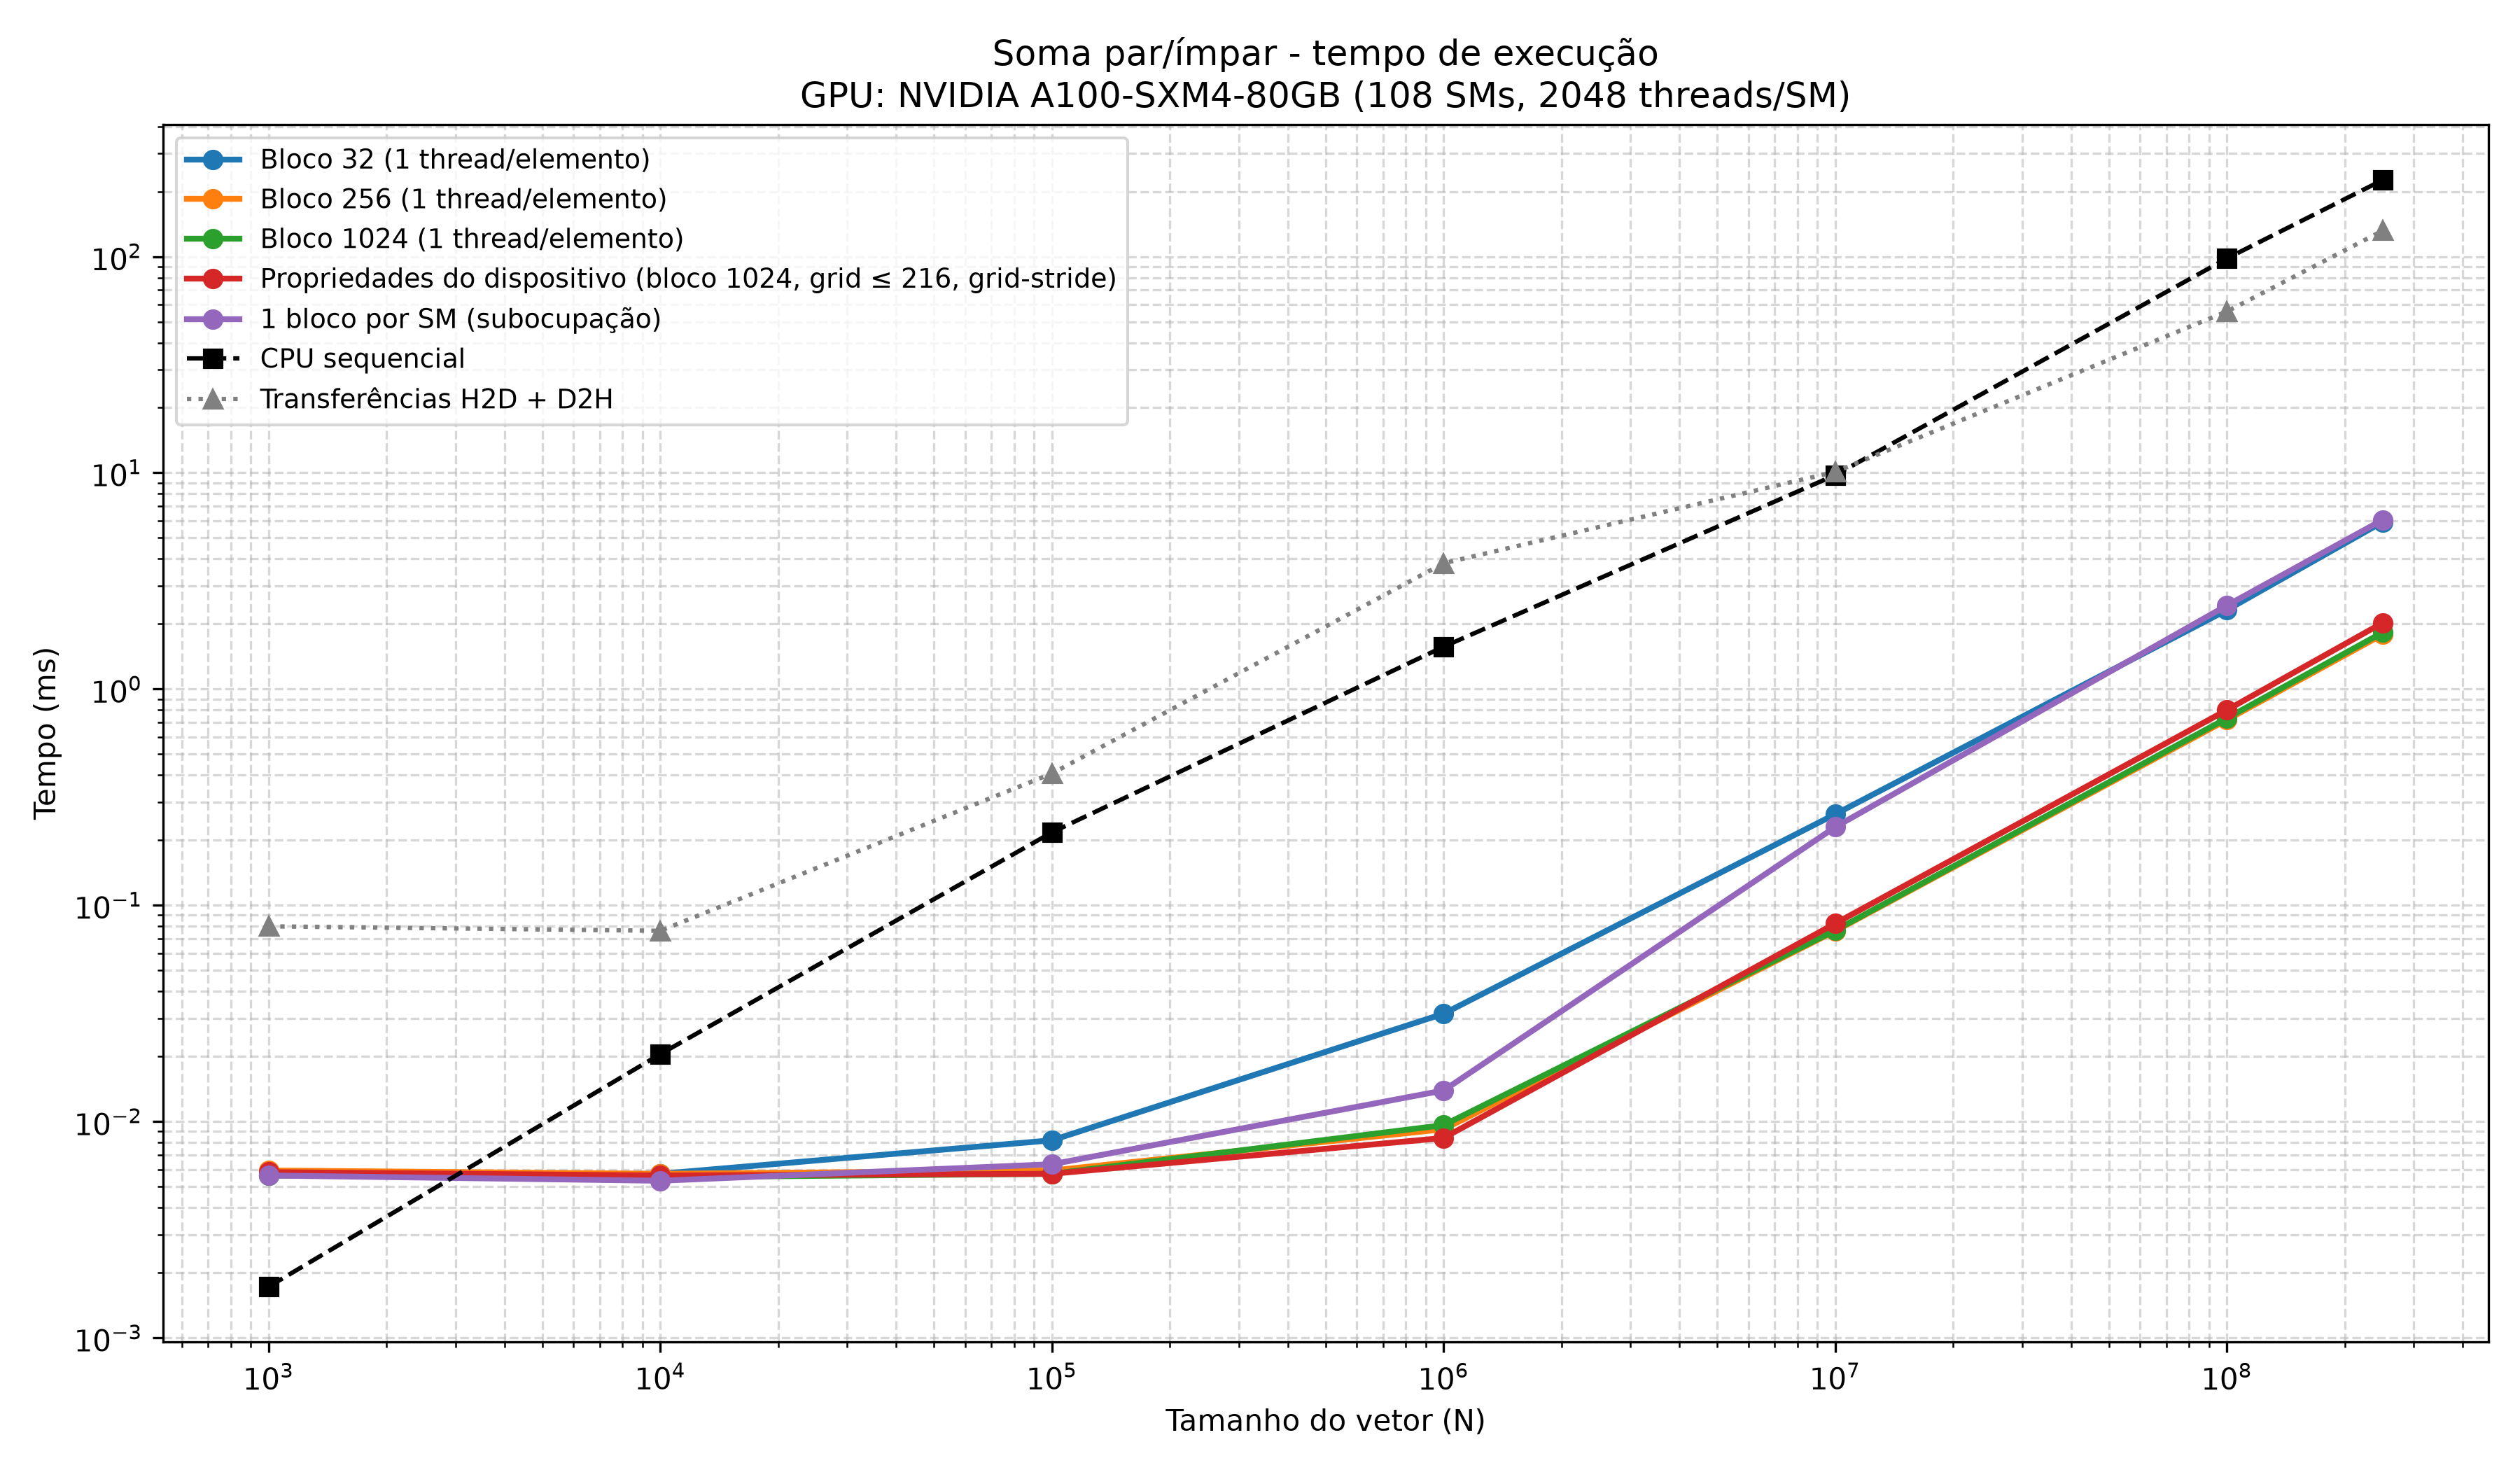
\includegraphics[width=\linewidth]{Tarefa16/tarefa16_tempos.png}
	\end{figure}
	\begin{figure}[H]
		\centering
		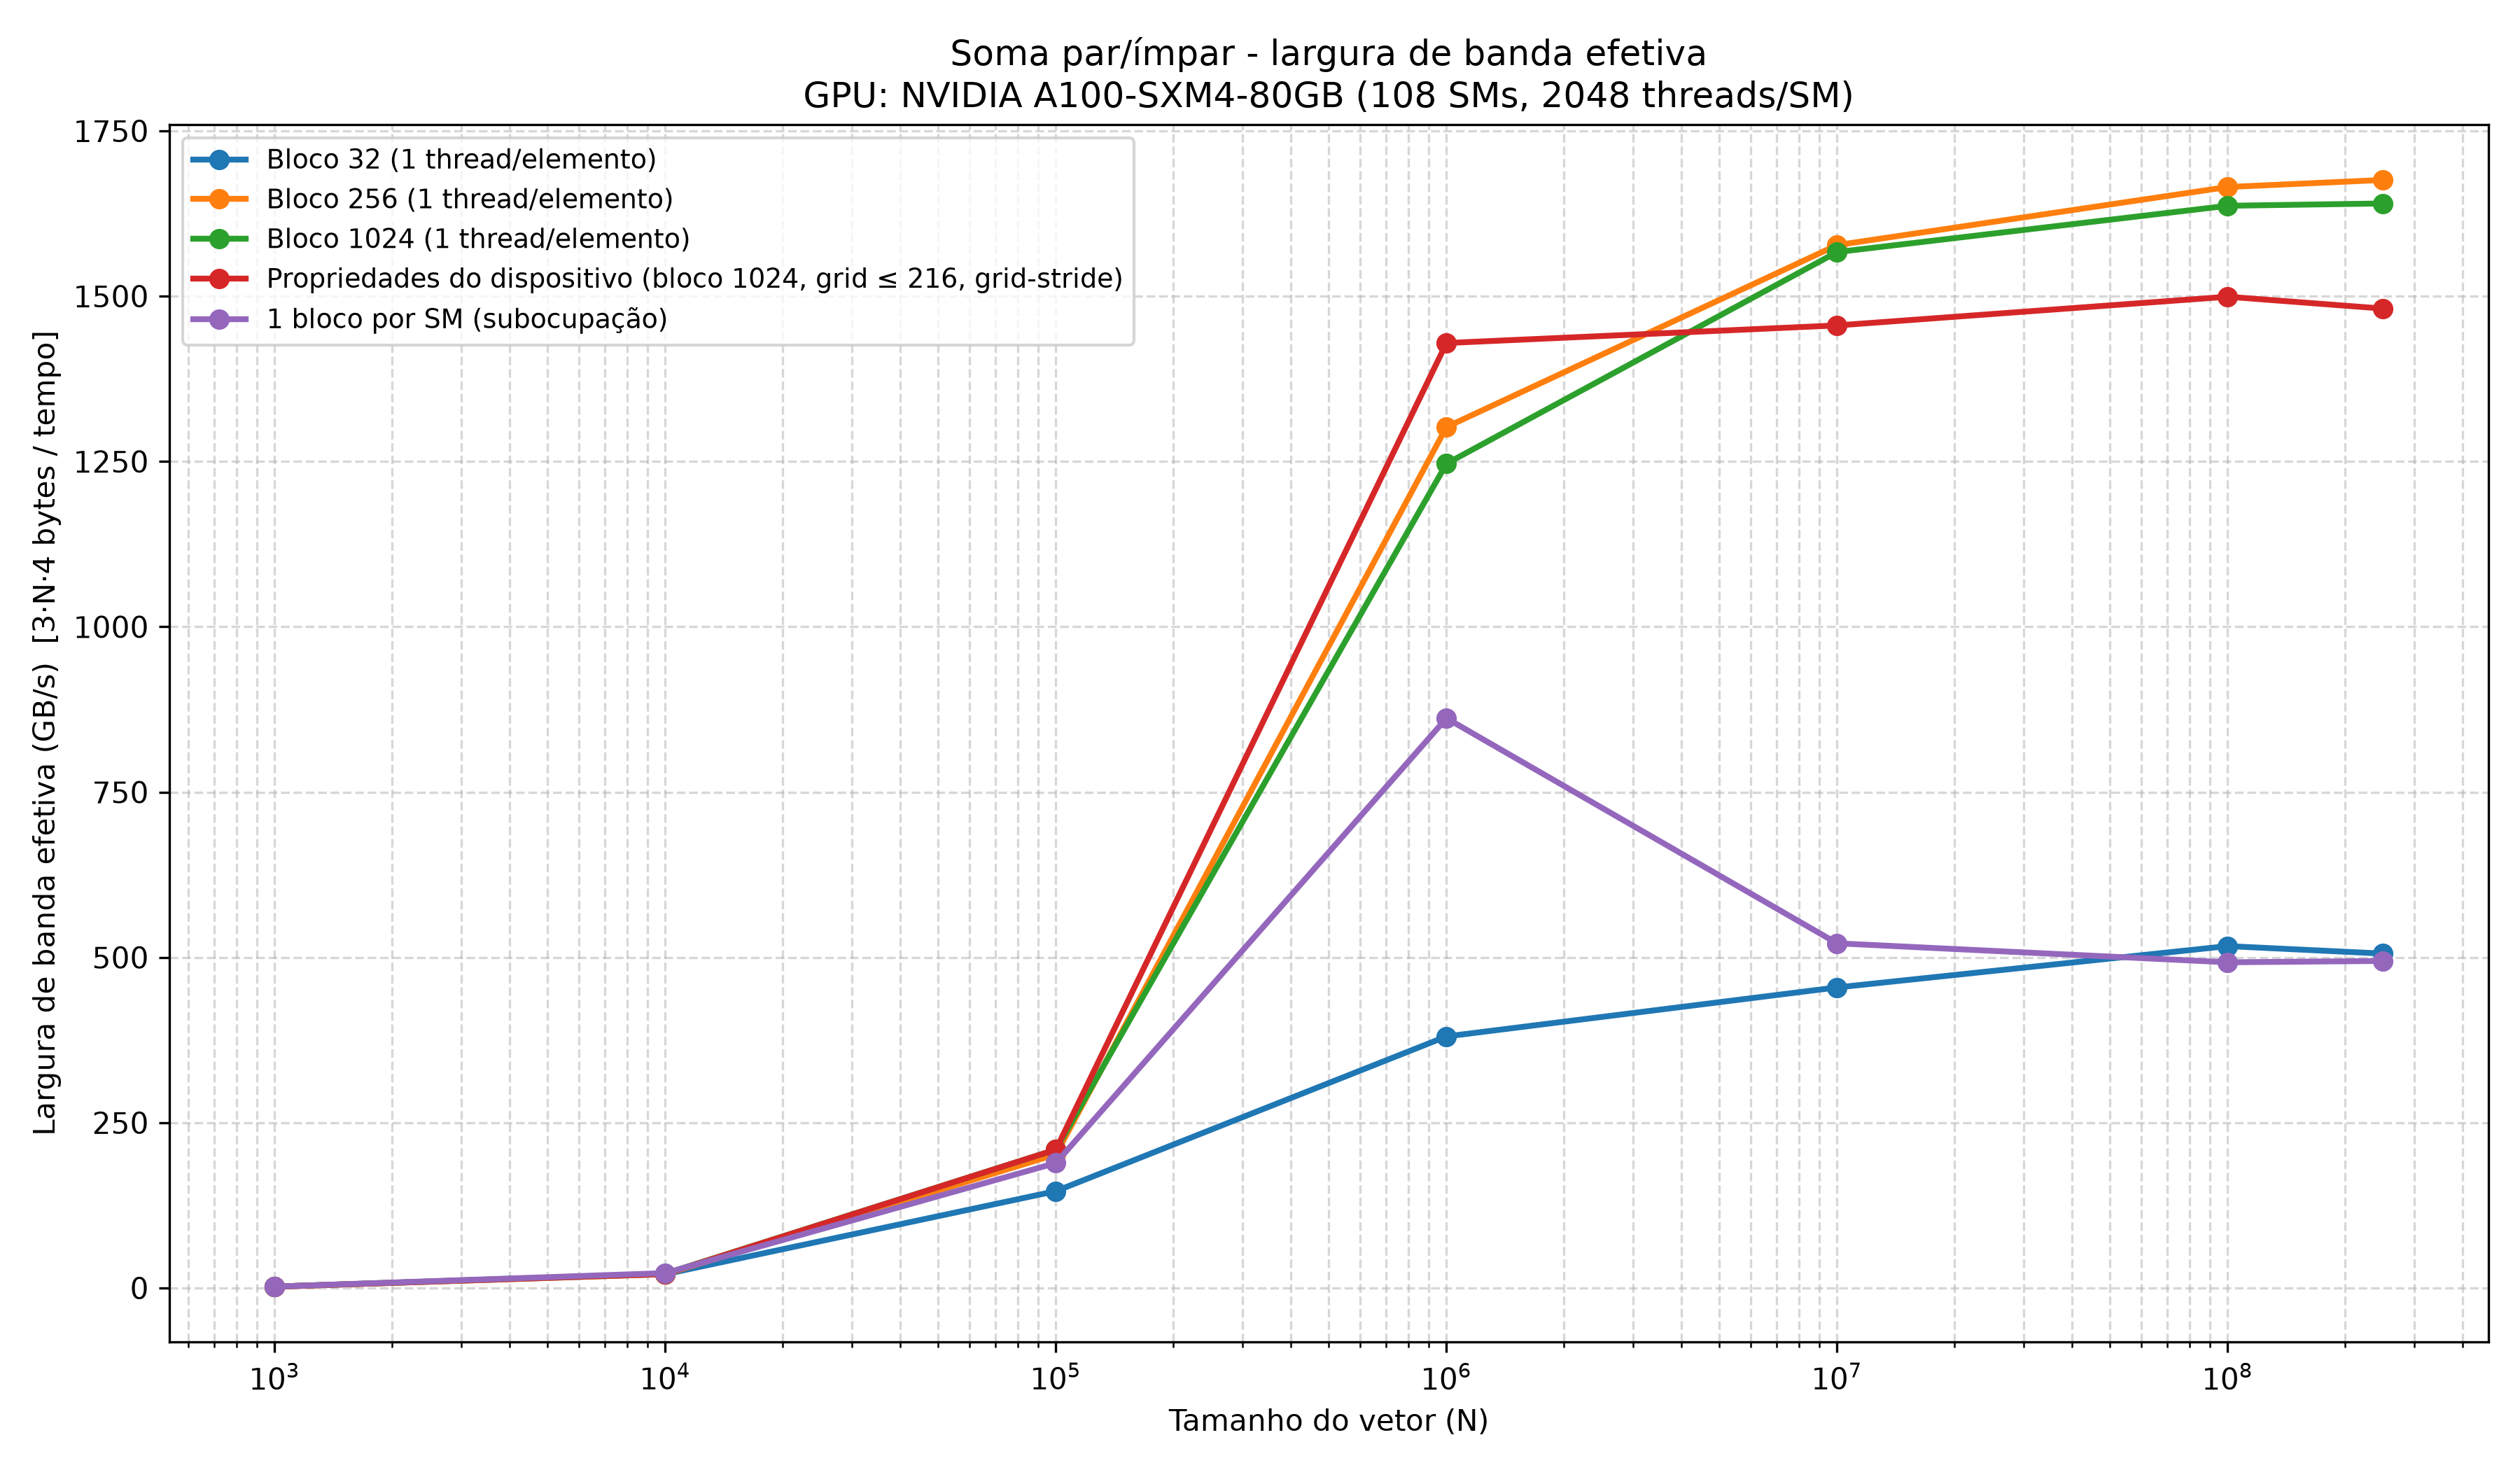
\includegraphics[width=\linewidth]{Tarefa16/tarefa16_banda.png}
	\end{figure}
	\begin{figure}[H]
		\centering
		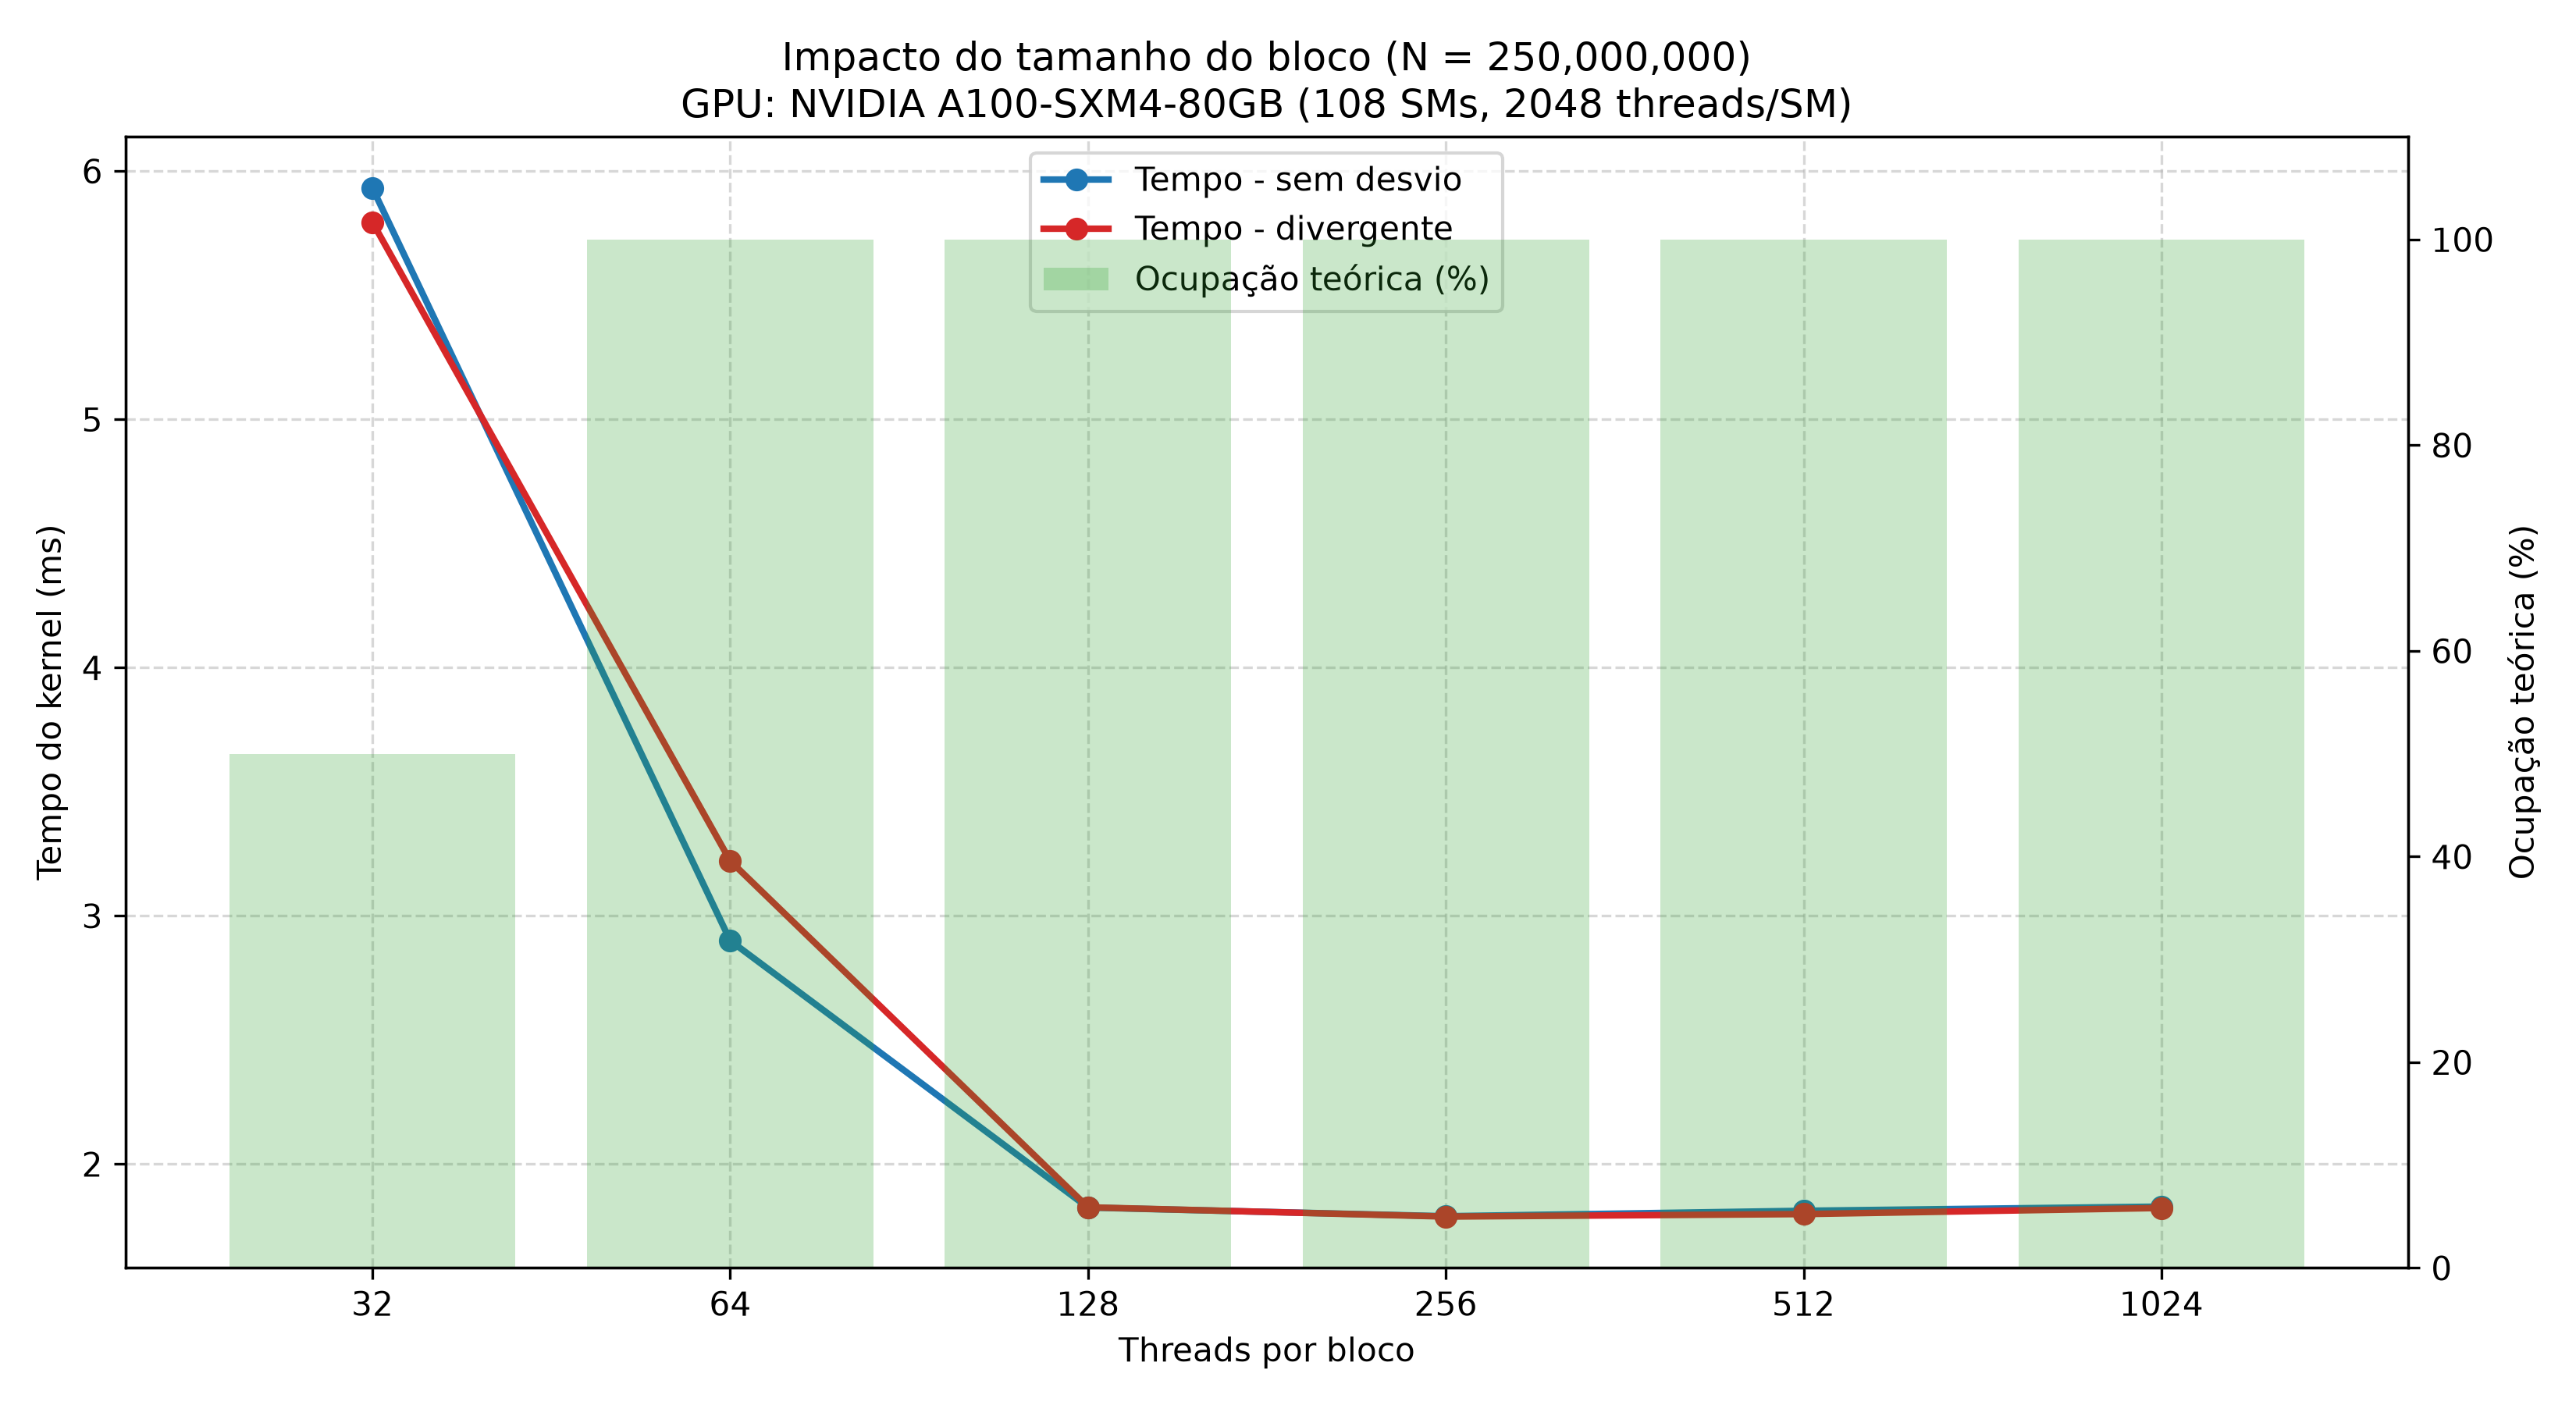
\includegraphics[width=\linewidth]{Tarefa16/tarefa16_blocos.png}
	\end{figure}
	\begin{figure}[H]
		\centering
		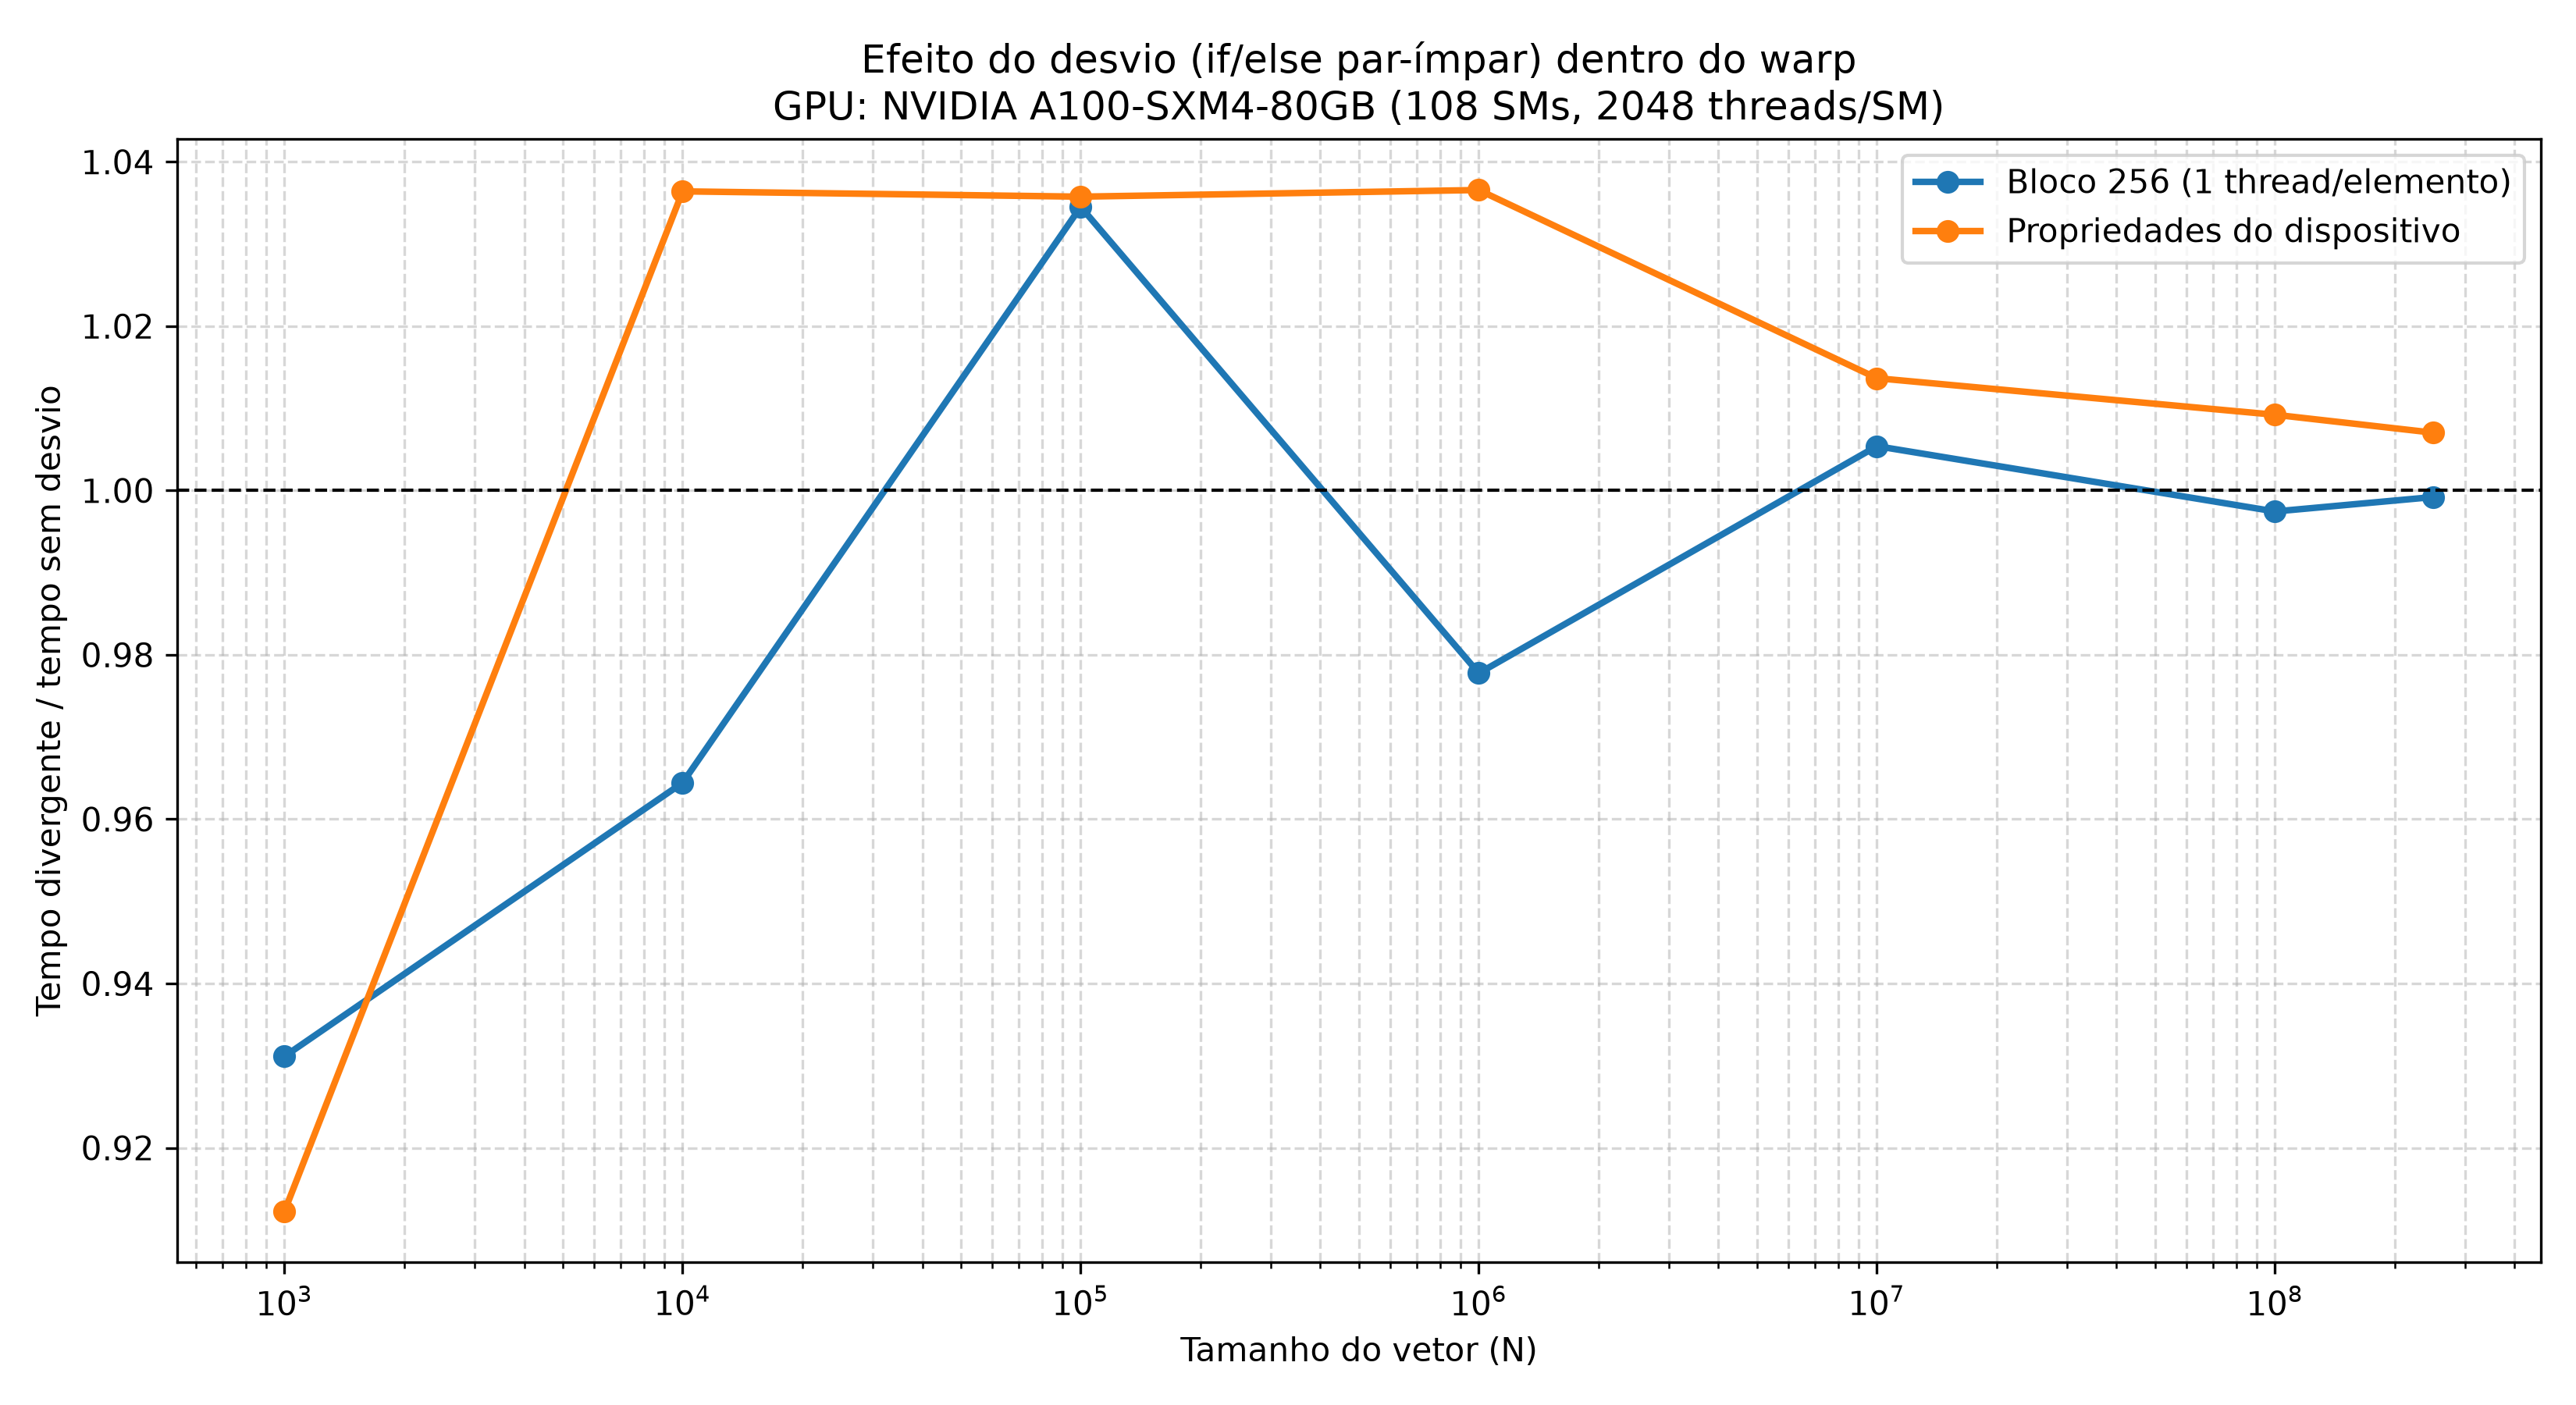
\includegraphics[width=\linewidth]{Tarefa16/tarefa16_divergencia.png}
	\end{figure}
	\par{
		A grid foi configurada a partir das propriedades da GPU A100 (108 SMs e até 2048 threads por SM), e comparada com blocos de 32 a 1024 threads, para vetores de mil a 250 milhões de elementos.
		
		Para vetores pequenos, todas as configurações levaram cerca de 5 microssegundos, que é apenas o custo de iniciar o kernel. Para os vetores grandes, blocos de 32 threads e a configuração com um bloco por SM tiveram baixa ocupação e foram cerca de 3 vezes mais lentos, enquanto blocos a partir de 128 threads atingiram o limite de banda da memória. A melhor configuração foi a de blocos de 256 threads, e a divergência entre pares e ímpares não fez diferença.
		
		Portanto, apesar de o kernel ser mais de 100 vezes mais rápido que a CPU, as transferências entre CPU e GPU levam muito mais tempo que o cálculo, e o uso da GPU só compensa quando os dados permanecem nela por várias operações.
	}
	\subsection{\subtTres}
	\begin{lstlisting}[language=c, title=kernel.cu]
#include <stdio.h>
#include <stdlib.h>
#include <math.h>
#include <time.h>

#define REPETICOES 10
#define ARQUIVO_JSON "resultados_cuda.json"

#define CUDA_CHECK(chamada)                                              \
    do {                                                                 \
        cudaError_t erro_ = (chamada);                                   \
        if (erro_ != cudaSuccess) {                                      \
            fprintf(stderr, "Erro CUDA %s:%d: %s\n", __FILE__, __LINE__, \
                    cudaGetErrorString(erro_));                          \
            exit(EXIT_FAILURE);                                          \
        }                                                                \
    } while (0)

static const size_t tamanhos[] = {
    1000,
    10000,
    100000,
    1000000,
    10000000,
    100000000,
    250000000,
};
static const size_t quantidade_tamanhos =
    sizeof(tamanhos) / sizeof(tamanhos[0]);

static const int blocos_testados[] = {32, 64, 128, 256, 512, 1024};
static const size_t quantidade_blocos =
    sizeof(blocos_testados) / sizeof(blocos_testados[0]);

static const char *classe_tamanho(size_t n)
{
    if (n <= 10000) return "pequeno";
    if (n <= 1000000) return "medio";
    return "grande";
}

__global__ void soma_divergente(const float *__restrict__ A,
                                const float *__restrict__ B,
                                float *__restrict__ C, size_t n)
{
    size_t i = (size_t)blockIdx.x * blockDim.x + threadIdx.x;
    size_t passo = (size_t)gridDim.x * blockDim.x;

    for (; i < n; i += passo) {
        if (i % 2 == 0) {
            C[i] = 2.0f * A[i] + B[i];
        } else {
            C[i] = A[i] + 3.0f * B[i];
        }
    }
}

__global__ void soma_sem_desvio(const float *__restrict__ A,
                                const float *__restrict__ B,
                                float *__restrict__ C, size_t n)
{
    size_t i = (size_t)blockIdx.x * blockDim.x + threadIdx.x;
    size_t passo = (size_t)gridDim.x * blockDim.x;

    for (; i < n; i += passo) {
        float impar = (float)(i & 1);
        C[i] = (2.0f - impar) * A[i] + (1.0f + 2.0f * impar) * B[i];
    }
}

static void soma_cpu(const float *A, const float *B, float *C, size_t n)
{
    for (size_t i = 0; i < n; i++) {
        if (i % 2 == 0) {
            C[i] = 2.0f * A[i] + B[i];
        } else {
            C[i] = A[i] + 3.0f * B[i];
        }
    }
}

static double tempo_atual(void)
{
    struct timespec ts;
    clock_gettime(CLOCK_MONOTONIC, &ts);
    return ts.tv_sec + ts.tv_nsec * 1e-9;
}

static size_t verifica(const float *ref, const float *gpu, size_t n)
{
    size_t erros = 0;
    for (size_t i = 0; i < n; i++) {
        float d = fabsf(ref[i] - gpu[i]);
        if (d > 1e-4f * fmaxf(1.0f, fabsf(ref[i]))) erros++;
    }
    return erros;
}

typedef void (*KernelSoma)(const float *, const float *, float *, size_t);

static float mede_kernel(KernelSoma kernel, int grid, int bloco,
                         const float *dA, const float *dB, float *dC,
                         size_t n, cudaEvent_t ini, cudaEvent_t fim)
{

    kernel<<<grid, bloco>>>(dA, dB, dC, n);
    CUDA_CHECK(cudaGetLastError());
    CUDA_CHECK(cudaDeviceSynchronize());

    float soma = 0.0f;
    for (int r = 0; r < REPETICOES; r++) {
        float ms = 0.0f;
        CUDA_CHECK(cudaEventRecord(ini));
        kernel<<<grid, bloco>>>(dA, dB, dC, n);
        CUDA_CHECK(cudaEventRecord(fim));
        CUDA_CHECK(cudaEventSynchronize(fim));
        CUDA_CHECK(cudaEventElapsedTime(&ms, ini, fim));
        soma += ms;
    }
    return soma / REPETICOES;
}

static double ocupacao_teorica(KernelSoma kernel, int bloco,
                               const cudaDeviceProp *prop, int *blocos_sm)
{
    CUDA_CHECK(cudaOccupancyMaxActiveBlocksPerMultiprocessor(
        blocos_sm, kernel, bloco, 0));
    return 100.0 * (*blocos_sm * bloco) / prop->maxThreadsPerMultiProcessor;
}

static int primeiro_registro = 1;

static void escreve_registro(FILE *json, size_t n, const char *config,
                             const char *kernel, int bloco, int grid,
                             double ocupacao, float tempo_ms, size_t erros)
{
    double bytes = 3.0 * n * sizeof(float);
    double banda = bytes / (tempo_ms * 1e-3) / 1e9;

    fprintf(json,
            "%s    {\"n\": %zu, \"classe\": \"%s\", \"config\": \"%s\", "
            "\"kernel\": \"%s\", \"bloco\": %d, \"grid\": %d, "
            "\"ocupacao_teorica_pct\": %.2f, \"tempo_kernel_ms\": %f, "
            "\"banda_gbs\": %f, \"erros\": %zu}",
            primeiro_registro ? "" : ",\n", n, classe_tamanho(n), config,
            kernel, bloco, grid, ocupacao, tempo_ms, banda, erros);
    primeiro_registro = 0;

    printf("  %-22s %-12s bloco %4d grid %9d | ocup %6.2f%% | "
           "%10.4f ms | %8.2f GB/s | erros %zu\n",
           config, kernel, bloco, grid, ocupacao, tempo_ms, banda, erros);
}

int main(void)
{

    int dispositivo = 0;
    cudaDeviceProp prop;
    CUDA_CHECK(cudaGetDevice(&dispositivo));
    CUDA_CHECK(cudaGetDeviceProperties(&prop, dispositivo));

    printf("GPU: %s | CC %d.%d | SMs: %d | max threads/SM: %d | "
           "max threads/bloco: %d | warp: %d\n",
           prop.name, prop.major, prop.minor, prop.multiProcessorCount,
           prop.maxThreadsPerMultiProcessor, prop.maxThreadsPerBlock,
           prop.warpSize);

    int grid_min = 0, bloco_ocupacao = 0;
    CUDA_CHECK(cudaOccupancyMaxPotentialBlockSize(
        &grid_min, &bloco_ocupacao, soma_sem_desvio, 0, 0));

    int blocos_sm_ocupacao = 0;
    double ocup_api = ocupacao_teorica(soma_sem_desvio, bloco_ocupacao,
                                       &prop, &blocos_sm_ocupacao);

    int grid_dispositivo = prop.multiProcessorCount * blocos_sm_ocupacao;

    printf("API de ocupacao: bloco = %d, blocos ativos/SM = %d "
           "(ocupacao %.1f%%), grid persistente = %d blocos (%d SMs x %d)\n\n",
           bloco_ocupacao, blocos_sm_ocupacao, ocup_api, grid_dispositivo,
           prop.multiProcessorCount, blocos_sm_ocupacao);

    size_t n_max = 0;
    for (size_t t = 0; t < quantidade_tamanhos; t++)
        if (tamanhos[t] > n_max) n_max = tamanhos[t];

    size_t bytes_max = n_max * sizeof(float);

    float *hA, *hB, *hC, *hRef;
    CUDA_CHECK(cudaMallocHost(&hA, bytes_max));
    CUDA_CHECK(cudaMallocHost(&hB, bytes_max));
    CUDA_CHECK(cudaMallocHost(&hC, bytes_max));
    hRef = (float *)malloc(bytes_max);
    if (hRef == NULL) {
        fprintf(stderr, "Erro ao alocar memoria.\n");
        return 1;
    }

    for (size_t i = 0; i < n_max; i++) {
        hA[i] = (float)(i % 1000) * 0.5f;
        hB[i] = (float)(i % 777) * 0.25f;
    }

    float *dA, *dB, *dC;
    CUDA_CHECK(cudaMalloc(&dA, bytes_max));
    CUDA_CHECK(cudaMalloc(&dB, bytes_max));
    CUDA_CHECK(cudaMalloc(&dC, bytes_max));

    cudaEvent_t ini, fim;
    CUDA_CHECK(cudaEventCreate(&ini));
    CUDA_CHECK(cudaEventCreate(&fim));

    FILE *json = fopen(ARQUIVO_JSON, "w");
    if (json == NULL) {
        fprintf(stderr, "Erro ao abrir %s\n", ARQUIVO_JSON);
        return 1;
    }

    fprintf(json, "{\n");
    fprintf(json, "  \"gpu\": \"%s\",\n", prop.name);
    fprintf(json, "  \"compute_capability\": \"%d.%d\",\n", prop.major,
            prop.minor);
    fprintf(json, "  \"sms\": %d,\n", prop.multiProcessorCount);
    fprintf(json, "  \"max_threads_por_sm\": %d,\n",
            prop.maxThreadsPerMultiProcessor);
    fprintf(json, "  \"max_threads_por_bloco\": %d,\n",
            prop.maxThreadsPerBlock);
    fprintf(json, "  \"warp\": %d,\n", prop.warpSize);
    fprintf(json, "  \"bloco_api_ocupacao\": %d,\n", bloco_ocupacao);
    fprintf(json, "  \"grid_persistente\": %d,\n", grid_dispositivo);
    fprintf(json, "  \"ocupacao_api_pct\": %.2f,\n", ocup_api);
    fprintf(json, "  \"repeticoes\": %d,\n", REPETICOES);

    fprintf(json, "  \"base\": [\n");

    for (size_t t = 0; t < quantidade_tamanhos; t++) {
        size_t n = tamanhos[t];
        size_t bytes = n * sizeof(float);

        double t0 = tempo_atual();
        soma_cpu(hA, hB, hRef, n);
        double tempo_cpu_ms = (tempo_atual() - t0) * 1e3;

        float h2d = 0.0f, d2h = 0.0f;
        CUDA_CHECK(cudaEventRecord(ini));
        CUDA_CHECK(cudaMemcpy(dA, hA, bytes, cudaMemcpyHostToDevice));
        CUDA_CHECK(cudaMemcpy(dB, hB, bytes, cudaMemcpyHostToDevice));
        CUDA_CHECK(cudaEventRecord(fim));
        CUDA_CHECK(cudaEventSynchronize(fim));
        CUDA_CHECK(cudaEventElapsedTime(&h2d, ini, fim));

        CUDA_CHECK(cudaEventRecord(ini));
        CUDA_CHECK(cudaMemcpy(hC, dC, bytes, cudaMemcpyDeviceToHost));
        CUDA_CHECK(cudaEventRecord(fim));
        CUDA_CHECK(cudaEventSynchronize(fim));
        CUDA_CHECK(cudaEventElapsedTime(&d2h, ini, fim));

        fprintf(json,
                "    {\"n\": %zu, \"classe\": \"%s\", \"tempo_cpu_ms\": %f, "
                "\"tempo_h2d_ms\": %f, \"tempo_d2h_ms\": %f}%s\n",
                n, classe_tamanho(n), tempo_cpu_ms, h2d, d2h,
                t + 1 < quantidade_tamanhos ? "," : "");
    }
    fprintf(json, "  ],\n");

    fprintf(json, "  \"resultados\": [\n");

    for (size_t t = 0; t < quantidade_tamanhos; t++) {
        size_t n = tamanhos[t];
        size_t bytes = n * sizeof(float);

        printf("====== N = %zu (%s) ======\n", n, classe_tamanho(n));

        soma_cpu(hA, hB, hRef, n);
        CUDA_CHECK(cudaMemcpy(dA, hA, bytes, cudaMemcpyHostToDevice));
        CUDA_CHECK(cudaMemcpy(dB, hB, bytes, cudaMemcpyHostToDevice));

        for (size_t b = 0; b < quantidade_blocos; b++) {
            int bloco = blocos_testados[b];
            int grid = (int)((n + bloco - 1) / bloco);
            int blocos_sm;

            for (int k = 0; k < 2; k++) {
                KernelSoma kernel = k == 0 ? soma_sem_desvio
                                           : soma_divergente;
                double ocup = ocupacao_teorica(kernel, bloco, &prop,
                                               &blocos_sm);
                CUDA_CHECK(cudaMemset(dC, 0, bytes));
                float ms = mede_kernel(kernel, grid, bloco, dA, dB, dC, n,
                                       ini, fim);
                CUDA_CHECK(cudaMemcpy(hC, dC, bytes,
                                      cudaMemcpyDeviceToHost));
                escreve_registro(json, n, "uma_thread_por_elemento",
                                 k == 0 ? "sem_desvio" : "divergente",
                                 bloco, grid, ocup, ms,
                                 verifica(hRef, hC, n));
            }
        }

        {
            int bloco = bloco_ocupacao;
            int grid_necessario = (int)((n + bloco - 1) / bloco);
            int grid = grid_dispositivo < grid_necessario ? grid_dispositivo
                                                          : grid_necessario;
            for (int k = 0; k < 2; k++) {
                KernelSoma kernel = k == 0 ? soma_sem_desvio
                                           : soma_divergente;
                int blocos_sm;
                double ocup = ocupacao_teorica(kernel, bloco, &prop,
                                               &blocos_sm);
                CUDA_CHECK(cudaMemset(dC, 0, bytes));
                float ms = mede_kernel(kernel, grid, bloco, dA, dB, dC, n,
                                       ini, fim);
                CUDA_CHECK(cudaMemcpy(hC, dC, bytes,
                                      cudaMemcpyDeviceToHost));
                escreve_registro(json, n, "dispositivo_grid_stride",
                                 k == 0 ? "sem_desvio" : "divergente",
                                 bloco, grid, ocup, ms,
                                 verifica(hRef, hC, n));
            }
        }

        {
            int bloco = 256;
            int grid = prop.multiProcessorCount;
            double ocup = 100.0 * bloco / prop.maxThreadsPerMultiProcessor;
            CUDA_CHECK(cudaMemset(dC, 0, bytes));
            float ms = mede_kernel(soma_sem_desvio, grid, bloco, dA, dB, dC,
                                   n, ini, fim);
            CUDA_CHECK(cudaMemcpy(hC, dC, bytes, cudaMemcpyDeviceToHost));
            escreve_registro(json, n, "um_bloco_por_sm", "sem_desvio",
                             bloco, grid, ocup, ms, verifica(hRef, hC, n));
        }
    }

    fprintf(json, "\n  ]\n}\n");
    fclose(json);

    printf("\nResultados salvos em %s\n", ARQUIVO_JSON);

    CUDA_CHECK(cudaEventDestroy(ini));
    CUDA_CHECK(cudaEventDestroy(fim));
    CUDA_CHECK(cudaFree(dA));
    CUDA_CHECK(cudaFree(dB));
    CUDA_CHECK(cudaFree(dC));
    CUDA_CHECK(cudaFreeHost(hA));
    CUDA_CHECK(cudaFreeHost(hB));
    CUDA_CHECK(cudaFreeHost(hC));
    free(hRef);

    return 0;
}
\end{lstlisting}
	\begin{lstlisting}[language=bash, title=script\_cuda.sh]
#!/bin/bash
#SBATCH --job-name=CUDA_soma_akira
#SBATCH --output=saida%j.out
#SBATCH --error=erro%j.err
#SBATCH --partition=gpu-4-a100
#SBATCH --nodes=1
#SBATCH --ntasks=1
#SBATCH --cpus-per-task=1
#SBATCH --mem=16G
#SBATCH --gpus-per-node=1
#SBATCH --time=0-0:15

cd "${SLURM_SUBMIT_DIR:-.}"

carrega_cuda() {
    command -v nvcc > /dev/null 2>&1 && return 0
    if ! type module > /dev/null 2>&1; then
        for f in /etc/profile.d/modules.sh /etc/profile.d/lmod.sh /usr/share/lmod/lmod/init/bash; do
            [ -f "$f" ] && source "$f" && break
        done
    fi
    if type module > /dev/null 2>&1; then
        if [ -n "$CUDA_MODULE" ]; then
            module load "$CUDA_MODULE"
        else
            for padrao in 'cuda' 'nvhpc' 'nvidia'; do
                mod=$(module -t avail 2>&1 | grep -v ':$' | grep -vE '^(containers|softwares)/' | grep -i "$padrao" | sort -V | tail -n 1)
                if [ -n "$mod" ]; then
                    echo "Carregando modulo: $mod"
                    module load "$mod" && command -v nvcc > /dev/null 2>&1 && return 0
                fi
            done
        fi
    fi
    command -v nvcc > /dev/null 2>&1 && return 0
    for d in /usr/local/cuda/bin /usr/local/cuda-*/bin /opt/cuda/bin \
             /opt/nvidia/hpc_sdk/Linux_x86_64/*/compilers/bin \
             /opt/nvidia/hpc_sdk/Linux_x86_64/*/cuda/*/bin; do
        if [ -x "$d/nvcc" ]; then
            export PATH="$d:$PATH"
            return 0
        fi
    done
    return 1
}

if ! carrega_cuda; then
    echo "nvcc nao encontrado. Modulos disponiveis:" >&2
    module -t avail 2>&1 | grep -iE 'cuda|nvhpc|nvidia' >&2
    echo "Informe o modulo: sbatch --export=ALL,CUDA_MODULE=<nome> script_cuda.sh" >&2
    exit 1
fi

echo "===== Ambiente ====="
hostname
nvidia-smi --query-gpu=name,memory.total,driver_version --format=csv
nvcc --version | tail -n 1

mkdir -p outputs

echo "===== Build ====="
nvcc -O2 kernel.cu -o outputs/kernel || exit 1

echo "===== Execucao ====="
./outputs/kernel

echo "===== Graficos ====="
if command -v python3 > /dev/null 2>&1 && python3 -c "import matplotlib" 2> /dev/null; then
    python3 plot.py
else
    echo "matplotlib indisponivel: copie resultados_cuda.json e rode plot.py localmente."
fi
\end{lstlisting}
	
	\newpage
	\onehalfspacing
	\section{TAREFA 17}
	\subsection{\subtUm}
	\par{Implementar versões de um programa de envio de mensagens entre processos com MPI, onde o processo 0 envia uma mensagem para o processo 1, que imediatamente responde com o mesmo conteúdo.
		
		Medir o tempo total de execução de múltiplas trocas consecutivas de mensagens, registrando os tempos para diferentes tamanhos de conteúdo.
		
		Analisar com gráficos o comportamento identificado, identificando onde a latência domina e onde a largura de banda se torna o fator principal, explicando cada implementação e função.}
	\subsection{\subtDois}
	\begin{figure}[H]
		\centering
		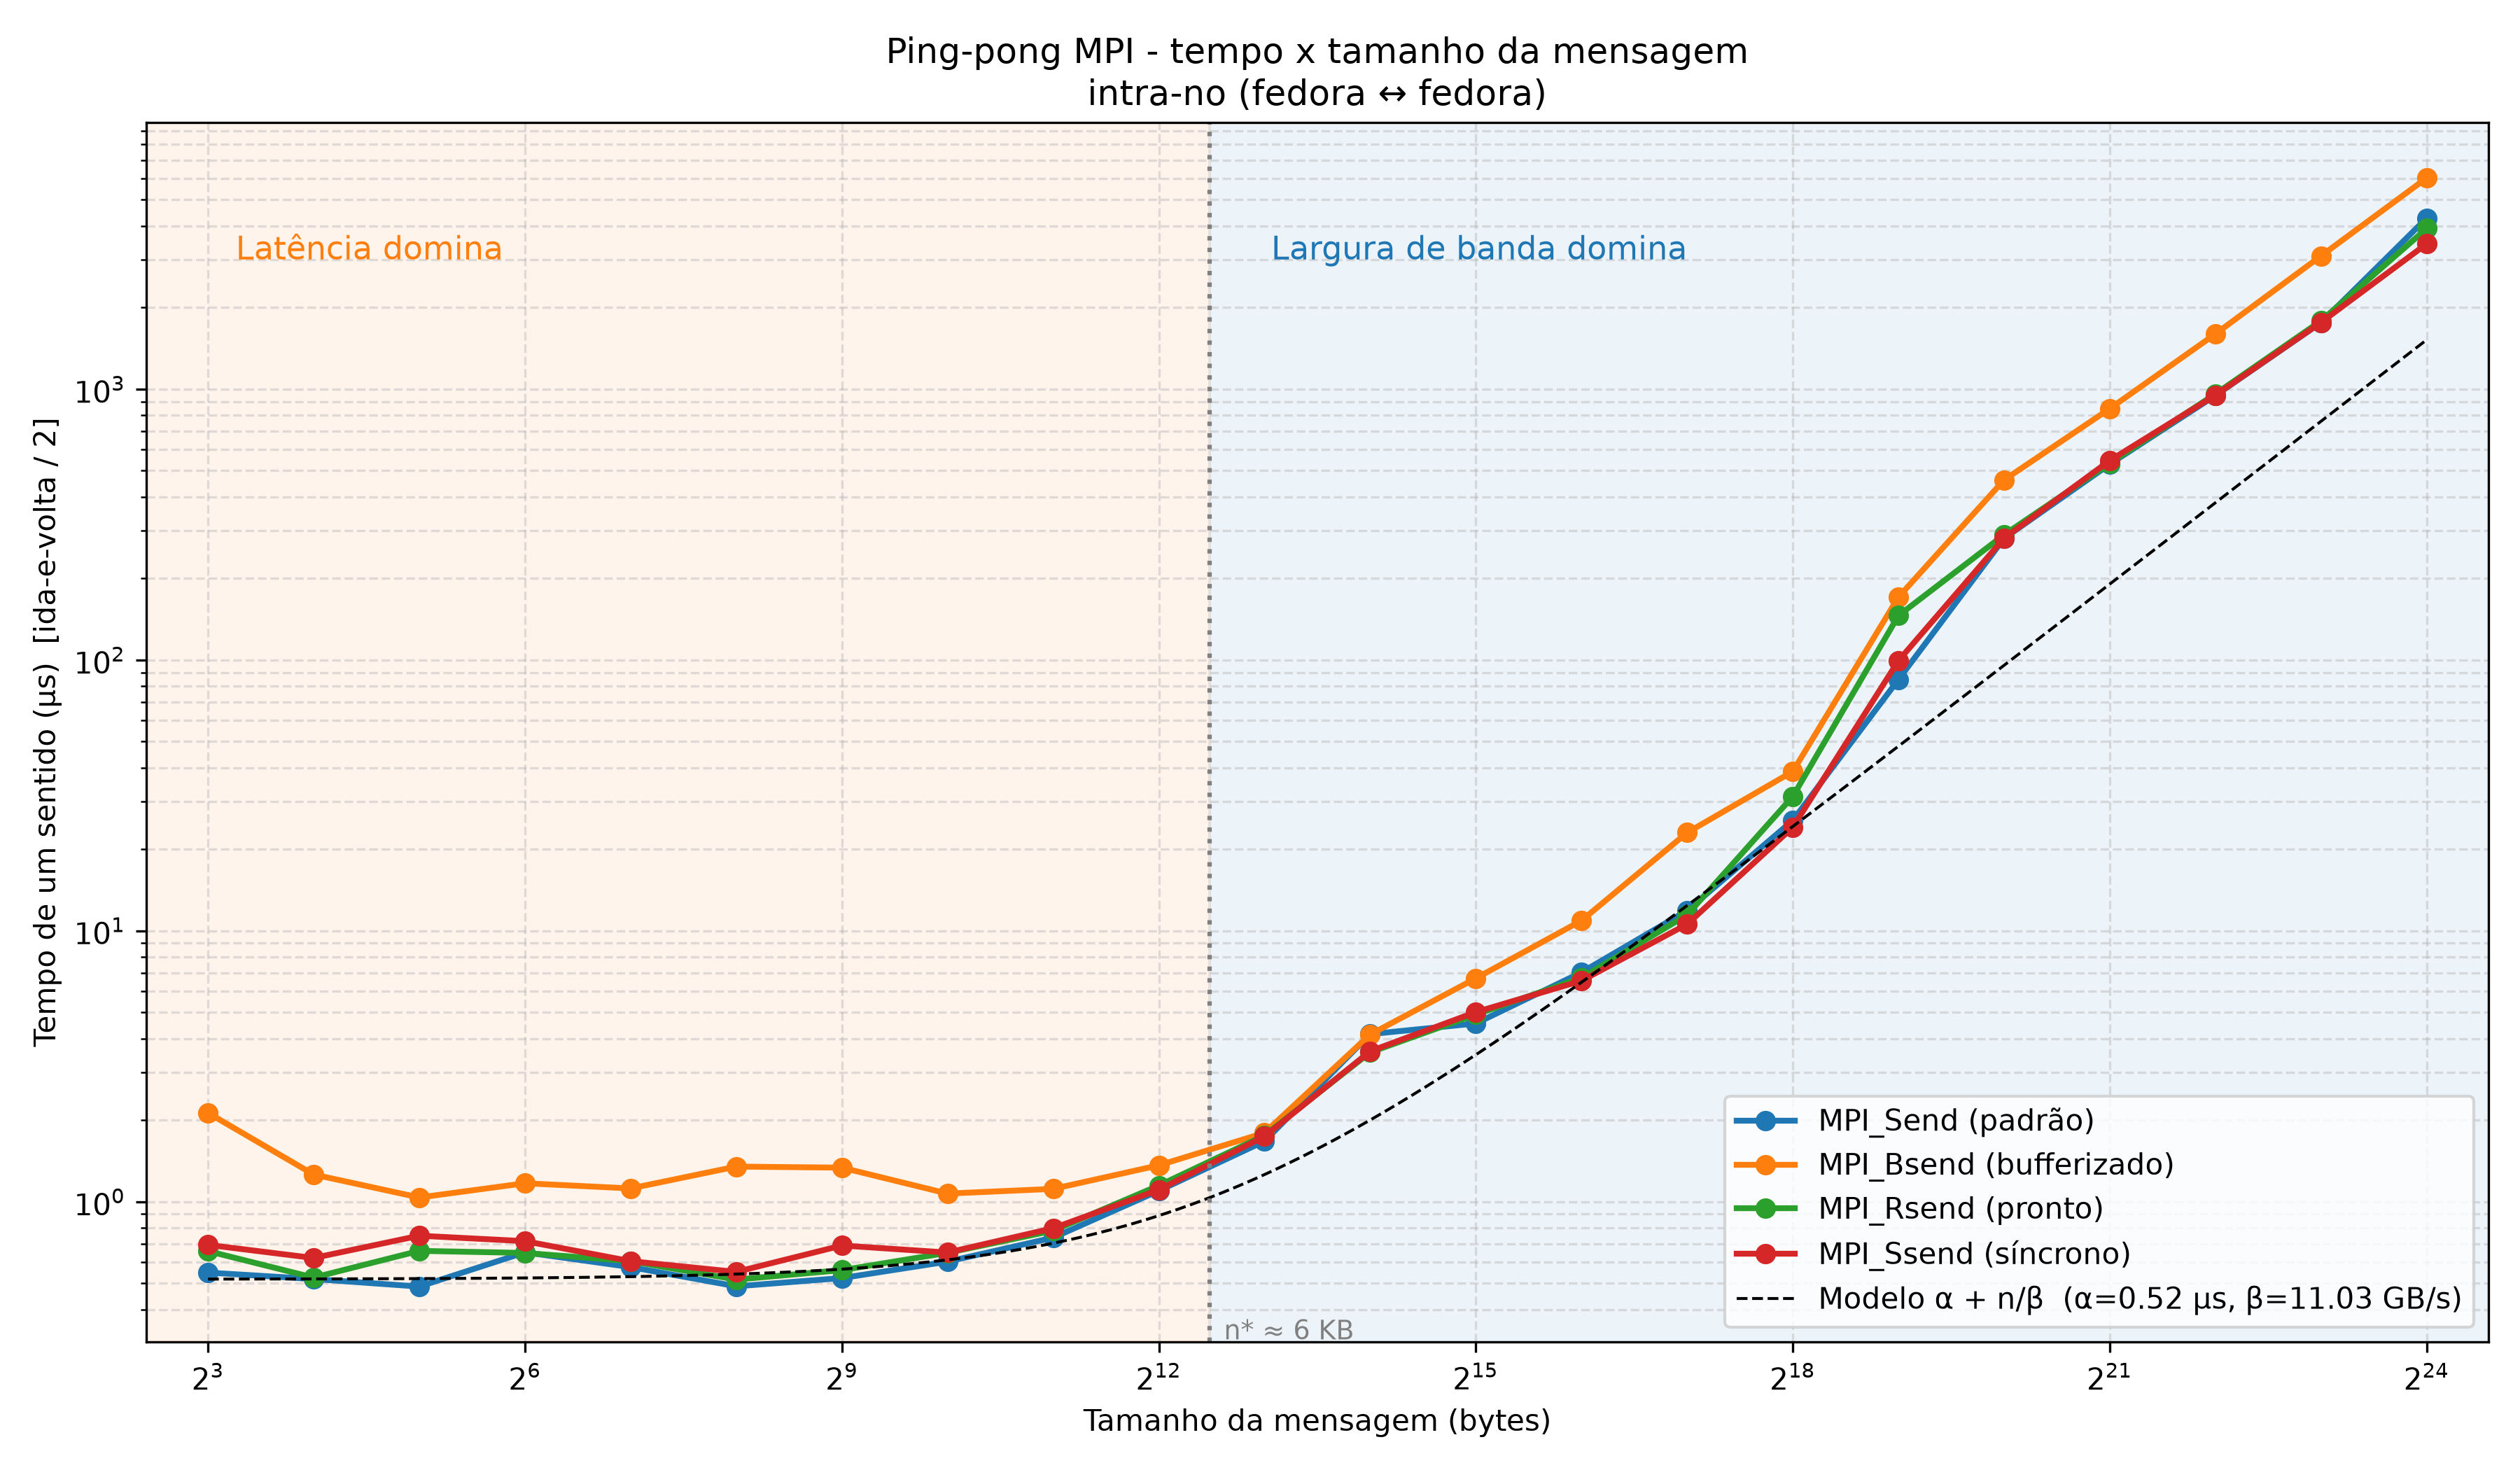
\includegraphics[width=\linewidth]{Tarefa17/tarefa17_tempo.png}
	\end{figure}
	\begin{figure}[H]
		\centering
		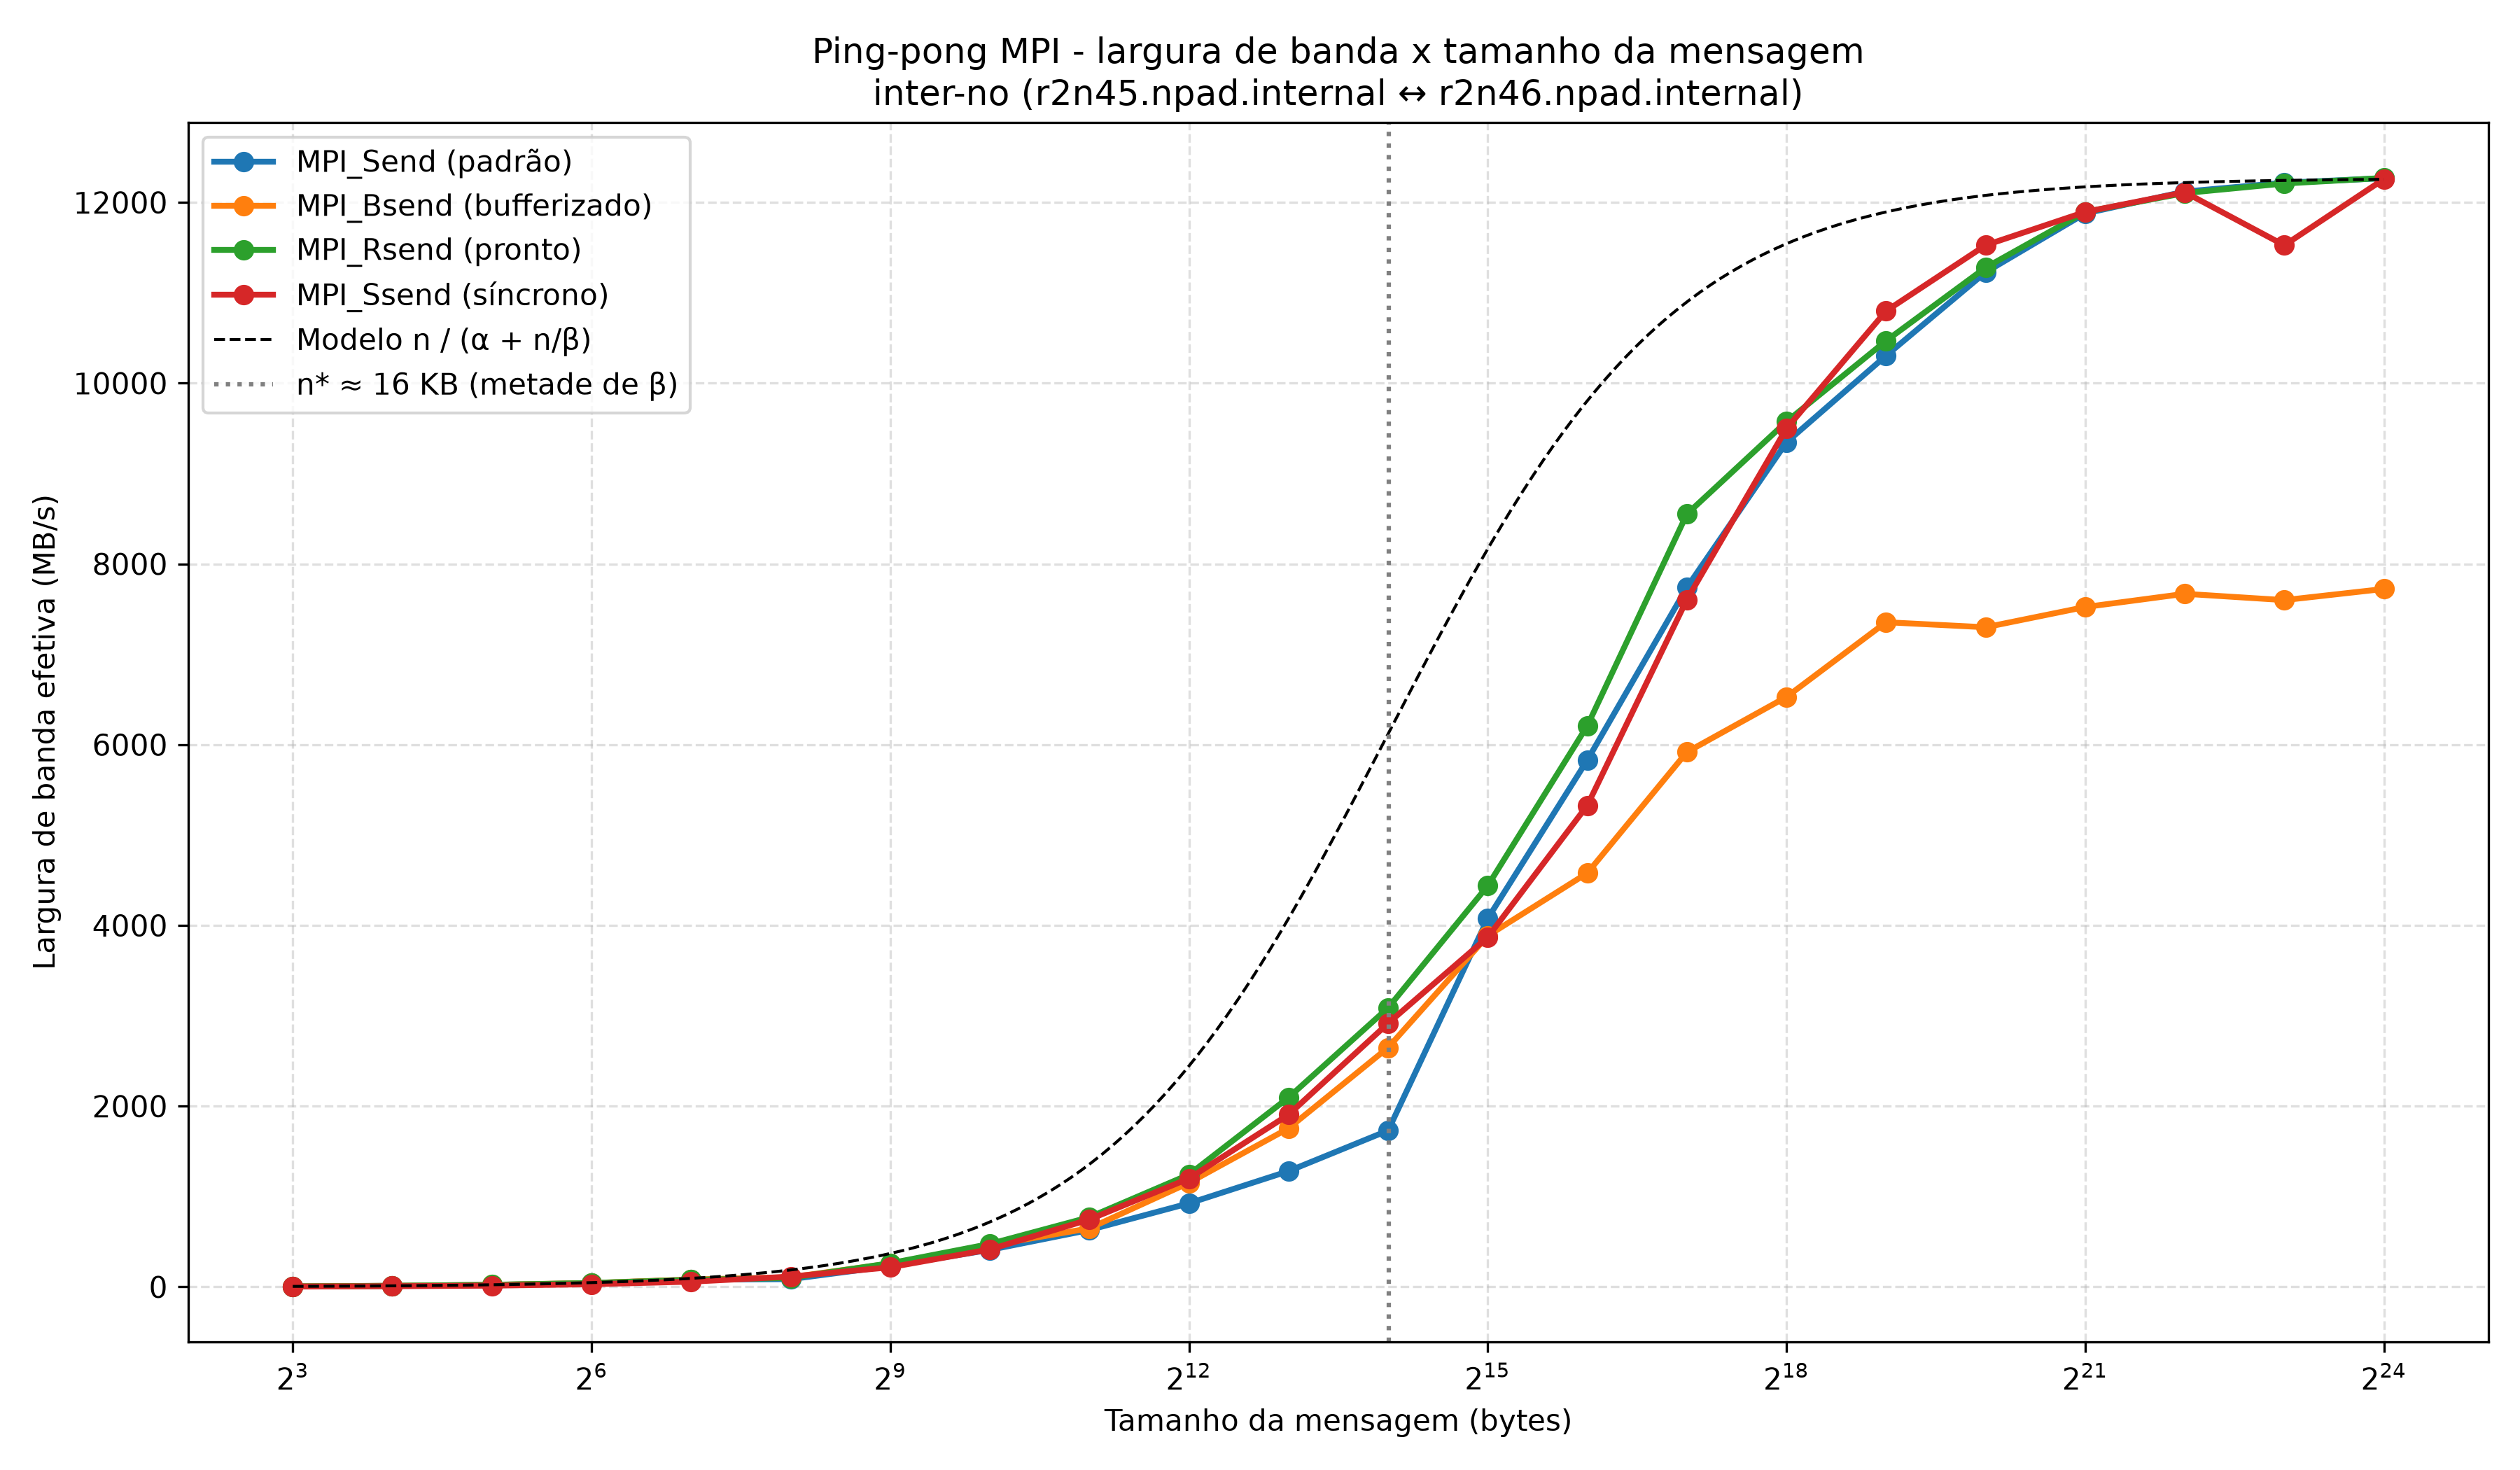
\includegraphics[width=\linewidth]{Tarefa17/tarefa17_banda.png}
	\end{figure}
	\par{
		Cada versão usa uma função de envio diferente: o MPI\_Send deixa a biblioteca decidir como enviar, o MPI\_Bsend copia a mensagem para um buffer próprio, o MPI\_Ssend espera o receptor começar a receber, e o MPI\_Rsend exige que o recebimento já esteja preparado.
		
		Analisando os gráficos, até cerca de 4 KB o tempo fica praticamente constante, perto de 0,5 microssegundo, e a latência domina. A partir de cerca de 8 KB, o tempo cresce junto com o tamanho da mensagem e a largura de banda passa a ser o fator principal, chegando a cerca de 10 GB/s.
		
		As versões com MPI\_Send, MPI\_Rsend e MPI\_Ssend tiveram desempenho parecido, com o Ssend um pouco mais lento em mensagens pequenas. O MPI\_Bsend foi o mais lento, por causa da cópia extra para o buffer. Portanto, o envio padrão é a melhor opção na maioria dos casos.
	}
	\subsection{\subtTres}
	\begin{lstlisting}[language=c, title=pingpong\_comum.h]
#ifndef PINGPONG_COMUM_H
#define PINGPONG_COMUM_H

#include <mpi.h>
#include <stdio.h>
#include <stdlib.h>
#include <string.h>

#define TAG_PING 10
#define TAG_PONG 20

#define AQUECIMENTO 10

static const size_t tamanhos[] = {
    8,       16,      32,      64,      128,     256,     512,
    1024,    2048,    4096,    8192,    16384,   32768,   65536,
    131072,  262144,  524288,  1048576, 2097152, 4194304, 8388608,
    16777216,
};
static const size_t quantidade_tamanhos =
    sizeof(tamanhos) / sizeof(tamanhos[0]);

static size_t maior_tamanho(void)
{
    size_t m = 0;
    for (size_t i = 0; i < quantidade_tamanhos; i++)
        if (tamanhos[i] > m) m = tamanhos[i];
    return m;
}

static int repeticoes_para(size_t bytes)
{
    if (bytes <= 65536) return 1000;
    size_t r = (64u * 1024u * 1024u) / bytes;
    return r < 20 ? 20 : (int)r;
}

static void troca_mensagens(char *envio, char *recepcao, char *recepcao2,
                            int bytes, int repeticoes, int rank);

static void prepara_modo(size_t maior_mensagem);
static void encerra_modo(void);

static int executa_pingpong(int argc, char *argv[], const char *modo,
                            const char *funcao)
{
    MPI_Init(&argc, &argv);

    int rank, processos;
    MPI_Comm_rank(MPI_COMM_WORLD, &rank);
    MPI_Comm_size(MPI_COMM_WORLD, &processos);

    if (processos != 2) {
        if (rank == 0)
            fprintf(stderr, "Este programa exige exatamente 2 processos "
                            "(recebeu %d).\n", processos);
        MPI_Finalize();
        return 1;
    }

    char no[MPI_MAX_PROCESSOR_NAME], no_outro[MPI_MAX_PROCESSOR_NAME];
    int tam_nome;
    memset(no, 0, sizeof(no));
    MPI_Get_processor_name(no, &tam_nome);
    if (rank == 0) {
        MPI_Recv(no_outro, MPI_MAX_PROCESSOR_NAME, MPI_CHAR, 1, 0,
                 MPI_COMM_WORLD, MPI_STATUS_IGNORE);
    } else {
        MPI_Send(no, MPI_MAX_PROCESSOR_NAME, MPI_CHAR, 0, 0, MPI_COMM_WORLD);
    }

    size_t maior = maior_tamanho();
    char *envio = malloc(maior);
    char *recepcao = malloc(maior);
    char *recepcao2 = malloc(maior);
    if (!envio || !recepcao || !recepcao2) {
        fprintf(stderr, "Erro ao alocar memoria.\n");
        MPI_Abort(MPI_COMM_WORLD, 1);
    }
    for (size_t i = 0; i < maior; i++) envio[i] = (char)(i % 251);

    prepara_modo(maior);

    char nome_arquivo[64];
    snprintf(nome_arquivo, sizeof(nome_arquivo), "resultados_%s.json", modo);

    FILE *json = NULL;
    if (rank == 0) {
        json = fopen(nome_arquivo, "w");
        if (json == NULL) {
            fprintf(stderr, "Erro ao abrir %s\n", nome_arquivo);
            MPI_Abort(MPI_COMM_WORLD, 1);
        }
        int mesmo_no = strcmp(no, no_outro) == 0;
        fprintf(json, "{\n");
        fprintf(json, "  \"modo\": \"%s\",\n", modo);
        fprintf(json, "  \"funcao\": \"%s\",\n", funcao);
        fprintf(json, "  \"no_processo_0\": \"%s\",\n", no);
        fprintf(json, "  \"no_processo_1\": \"%s\",\n", no_outro);
        fprintf(json, "  \"comunicacao\": \"%s\",\n",
                mesmo_no ? "intra-no" : "inter-no");
        fprintf(json, "  \"resultados\": [\n");

        printf("[%s] processo 0 em %s, processo 1 em %s (%s)\n", funcao, no,
               no_outro, mesmo_no ? "intra-no" : "inter-no");
        printf("%10s %8s %14s %14s %14s\n", "bytes", "reps", "total (s)",
               "latencia(us)", "banda (MB/s)");
    }

    for (size_t t = 0; t < quantidade_tamanhos; t++) {
        int bytes = (int)tamanhos[t];
        int repeticoes = repeticoes_para(tamanhos[t]);

        MPI_Barrier(MPI_COMM_WORLD);
        troca_mensagens(envio, recepcao, recepcao2, bytes, AQUECIMENTO, rank);

        memset(recepcao, 0, bytes);
        MPI_Barrier(MPI_COMM_WORLD);

        double inicio = MPI_Wtime();
        troca_mensagens(envio, recepcao, recepcao2, bytes, repeticoes, rank);
        double fim = MPI_Wtime();

        if (rank == 0) {

            int ok = memcmp(envio, recepcao, bytes) == 0;

            double total = fim - inicio;
            double ida_volta = total / repeticoes;
            double latencia = ida_volta / 2.0;
            double banda = bytes / latencia / 1e6;

            printf("%10d %8d %14.6f %14.3f %14.2f %s\n", bytes, repeticoes,
                   total, latencia * 1e6, banda, ok ? "" : "ERRO");

            fprintf(json,
                    "    {\"bytes\": %d, \"repeticoes\": %d, "
                    "\"tempo_total_s\": %.9f, \"tempo_ida_volta_us\": %.4f, "
                    "\"latencia_us\": %.4f, \"banda_mbs\": %.4f, "
                    "\"valido\": %s}%s\n",
                    bytes, repeticoes, total, ida_volta * 1e6, latencia * 1e6,
                    banda, ok ? "true" : "false",
                    t + 1 < quantidade_tamanhos ? "," : "");
        }
    }

    if (rank == 0) {
        fprintf(json, "  ]\n}\n");
        fclose(json);
        printf("Resultados salvos em %s\n", nome_arquivo);
    }

    encerra_modo();

    free(envio);
    free(recepcao);
    free(recepcao2);

    MPI_Finalize();
    return 0;
}

#endif
\end{lstlisting}
	\begin{lstlisting}[language=c, title=pingpong\_send.c]
#include "pingpong_comum.h"

static void prepara_modo(size_t maior_mensagem) { (void)maior_mensagem; }
static void encerra_modo(void) {}

static void troca_mensagens(char *envio, char *recepcao, char *recepcao2,
                            int bytes, int repeticoes, int rank)
{
    (void)recepcao2;

    for (int i = 0; i < repeticoes; i++) {
        if (rank == 0) {

            MPI_Send(envio, bytes, MPI_CHAR, 1, TAG_PING, MPI_COMM_WORLD);

            MPI_Recv(recepcao, bytes, MPI_CHAR, 1, TAG_PONG, MPI_COMM_WORLD,
                     MPI_STATUS_IGNORE);
        } else {
            MPI_Recv(recepcao, bytes, MPI_CHAR, 0, TAG_PING, MPI_COMM_WORLD,
                     MPI_STATUS_IGNORE);

            MPI_Send(recepcao, bytes, MPI_CHAR, 0, TAG_PONG, MPI_COMM_WORLD);
        }
    }
}

int main(int argc, char *argv[])
{
    return executa_pingpong(argc, argv, "send", "MPI_Send");
}
\end{lstlisting}
	\begin{lstlisting}[language=c, title=pingpong\_bsend.c]
#include "pingpong_comum.h"

static void *buffer_bsend = NULL;

static void prepara_modo(size_t maior_mensagem)
{

    int tamanho = (int)(2 * (maior_mensagem + MPI_BSEND_OVERHEAD));
    buffer_bsend = malloc(tamanho);
    if (buffer_bsend == NULL) {
        fprintf(stderr, "Erro ao alocar buffer do MPI_Bsend.\n");
        MPI_Abort(MPI_COMM_WORLD, 1);
    }
    MPI_Buffer_attach(buffer_bsend, tamanho);
}

static void encerra_modo(void)
{
    void *endereco;
    int tamanho;

    MPI_Buffer_detach(&endereco, &tamanho);
    free(buffer_bsend);
}

static void troca_mensagens(char *envio, char *recepcao, char *recepcao2,
                            int bytes, int repeticoes, int rank)
{
    (void)recepcao2;

    for (int i = 0; i < repeticoes; i++) {
        if (rank == 0) {
            MPI_Bsend(envio, bytes, MPI_CHAR, 1, TAG_PING, MPI_COMM_WORLD);
            MPI_Recv(recepcao, bytes, MPI_CHAR, 1, TAG_PONG, MPI_COMM_WORLD,
                     MPI_STATUS_IGNORE);
        } else {
            MPI_Recv(recepcao, bytes, MPI_CHAR, 0, TAG_PING, MPI_COMM_WORLD,
                     MPI_STATUS_IGNORE);
            MPI_Bsend(recepcao, bytes, MPI_CHAR, 0, TAG_PONG, MPI_COMM_WORLD);
        }
    }
}

int main(int argc, char *argv[])
{
    return executa_pingpong(argc, argv, "bsend", "MPI_Bsend");
}
\end{lstlisting}
	\begin{lstlisting}[language=c, title=pingpong\_rsend.c]
#include "pingpong_comum.h"

static void prepara_modo(size_t maior_mensagem) { (void)maior_mensagem; }
static void encerra_modo(void) {}

static void troca_mensagens(char *envio, char *recepcao, char *recepcao2,
                            int bytes, int repeticoes, int rank)
{
    MPI_Request req;

    if (rank == 0) {
        MPI_Barrier(MPI_COMM_WORLD);

        for (int i = 0; i < repeticoes; i++) {
            MPI_Irecv(recepcao, bytes, MPI_CHAR, 1, TAG_PONG, MPI_COMM_WORLD,
                      &req);
            MPI_Rsend(envio, bytes, MPI_CHAR, 1, TAG_PING, MPI_COMM_WORLD);
            MPI_Wait(&req, MPI_STATUS_IGNORE);
        }
    } else {
        char *buffers[2] = {recepcao, recepcao2};
        int atual = 0;

        MPI_Irecv(buffers[atual], bytes, MPI_CHAR, 0, TAG_PING,
                  MPI_COMM_WORLD, &req);
        MPI_Barrier(MPI_COMM_WORLD);

        for (int i = 0; i < repeticoes; i++) {
            MPI_Wait(&req, MPI_STATUS_IGNORE);
            char *recebido = buffers[atual];

            if (i + 1 < repeticoes) {
                atual = 1 - atual;
                MPI_Irecv(buffers[atual], bytes, MPI_CHAR, 0, TAG_PING,
                          MPI_COMM_WORLD, &req);
            }

            MPI_Rsend(recebido, bytes, MPI_CHAR, 0, TAG_PONG, MPI_COMM_WORLD);
        }
    }
}

int main(int argc, char *argv[])
{
    return executa_pingpong(argc, argv, "rsend", "MPI_Rsend");
}
\end{lstlisting}
	\begin{lstlisting}[language=c, title=pingpong\_ssend.c]
#include "pingpong_comum.h"

static void prepara_modo(size_t maior_mensagem) { (void)maior_mensagem; }
static void encerra_modo(void) {}

static void troca_mensagens(char *envio, char *recepcao, char *recepcao2,
                            int bytes, int repeticoes, int rank)
{
    (void)recepcao2;

    for (int i = 0; i < repeticoes; i++) {
        if (rank == 0) {
            MPI_Ssend(envio, bytes, MPI_CHAR, 1, TAG_PING, MPI_COMM_WORLD);
            MPI_Recv(recepcao, bytes, MPI_CHAR, 1, TAG_PONG, MPI_COMM_WORLD,
                     MPI_STATUS_IGNORE);
        } else {
            MPI_Recv(recepcao, bytes, MPI_CHAR, 0, TAG_PING, MPI_COMM_WORLD,
                     MPI_STATUS_IGNORE);
            MPI_Ssend(recepcao, bytes, MPI_CHAR, 0, TAG_PONG, MPI_COMM_WORLD);
        }
    }
}

int main(int argc, char *argv[])
{
    return executa_pingpong(argc, argv, "ssend", "MPI_Ssend");
}
\end{lstlisting}
	\begin{lstlisting}[language=bash, title=script\_mpi.sh]
#!/bin/bash
#SBATCH --job-name=MPI_pingpong_akira
#SBATCH --output=saida%j.out
#SBATCH --error=erro%j.err
#SBATCH --partition=amd-512
#SBATCH --nodes=2
#SBATCH --ntasks-per-node=1
#SBATCH --time=0-0:15

cd "${SLURM_SUBMIT_DIR:-.}"
mkdir -p outputs

MPIRUN_OPTS=""
if mpirun --version 2>&1 | grep -qi "open mpi"; then
    MPIRUN_OPTS="--mca btl ^openib"
fi

echo "===== Build ====="
for modo in send bsend rsend ssend; do
    mpicc -O2 pingpong_${modo}.c -o outputs/pingpong_${modo} || exit 1
done

for modo in send bsend rsend ssend; do
    echo "===== MPI_${modo^} ====="
    mpirun -np 2 ${MPIRUN_OPTS} ./outputs/pingpong_${modo}
done

echo "===== Graficos ====="
if command -v python3 > /dev/null 2>&1 && python3 -c "import matplotlib" 2> /dev/null; then
    python3 plot.py
else
    echo "matplotlib indisponivel: copie os resultados_*.json e rode plot.py localmente."
fi
\end{lstlisting}
	
	\newpage
	\onehalfspacing
	\section{TAREFA 18}
	\subsection{\subtUm}
	\par{Adaptar o código de propagação de onda para que cada fonte sísmica seja processada de forma independente por um processo MPI através de um escalonador dinâmico com o modelo Master-Worker.
		
		O processo líder deve enviar um struct com a posição da fonte sísmica pra ser processada. Cada trabalhador processa os dados recebidos e enviar uma mensagem ao líder indicando o resultado, que irá então atualizar a informação para atribuir uma nova tarefa ao trabalhador.
		
		Apresentar os resultados, variando a quantidade de fontes a serem processadas, analisando o comportamento do escalonador em função da quantidade de tiros.}
	\subsection{\subtDois}
	\begin{figure}[H]
		\centering
		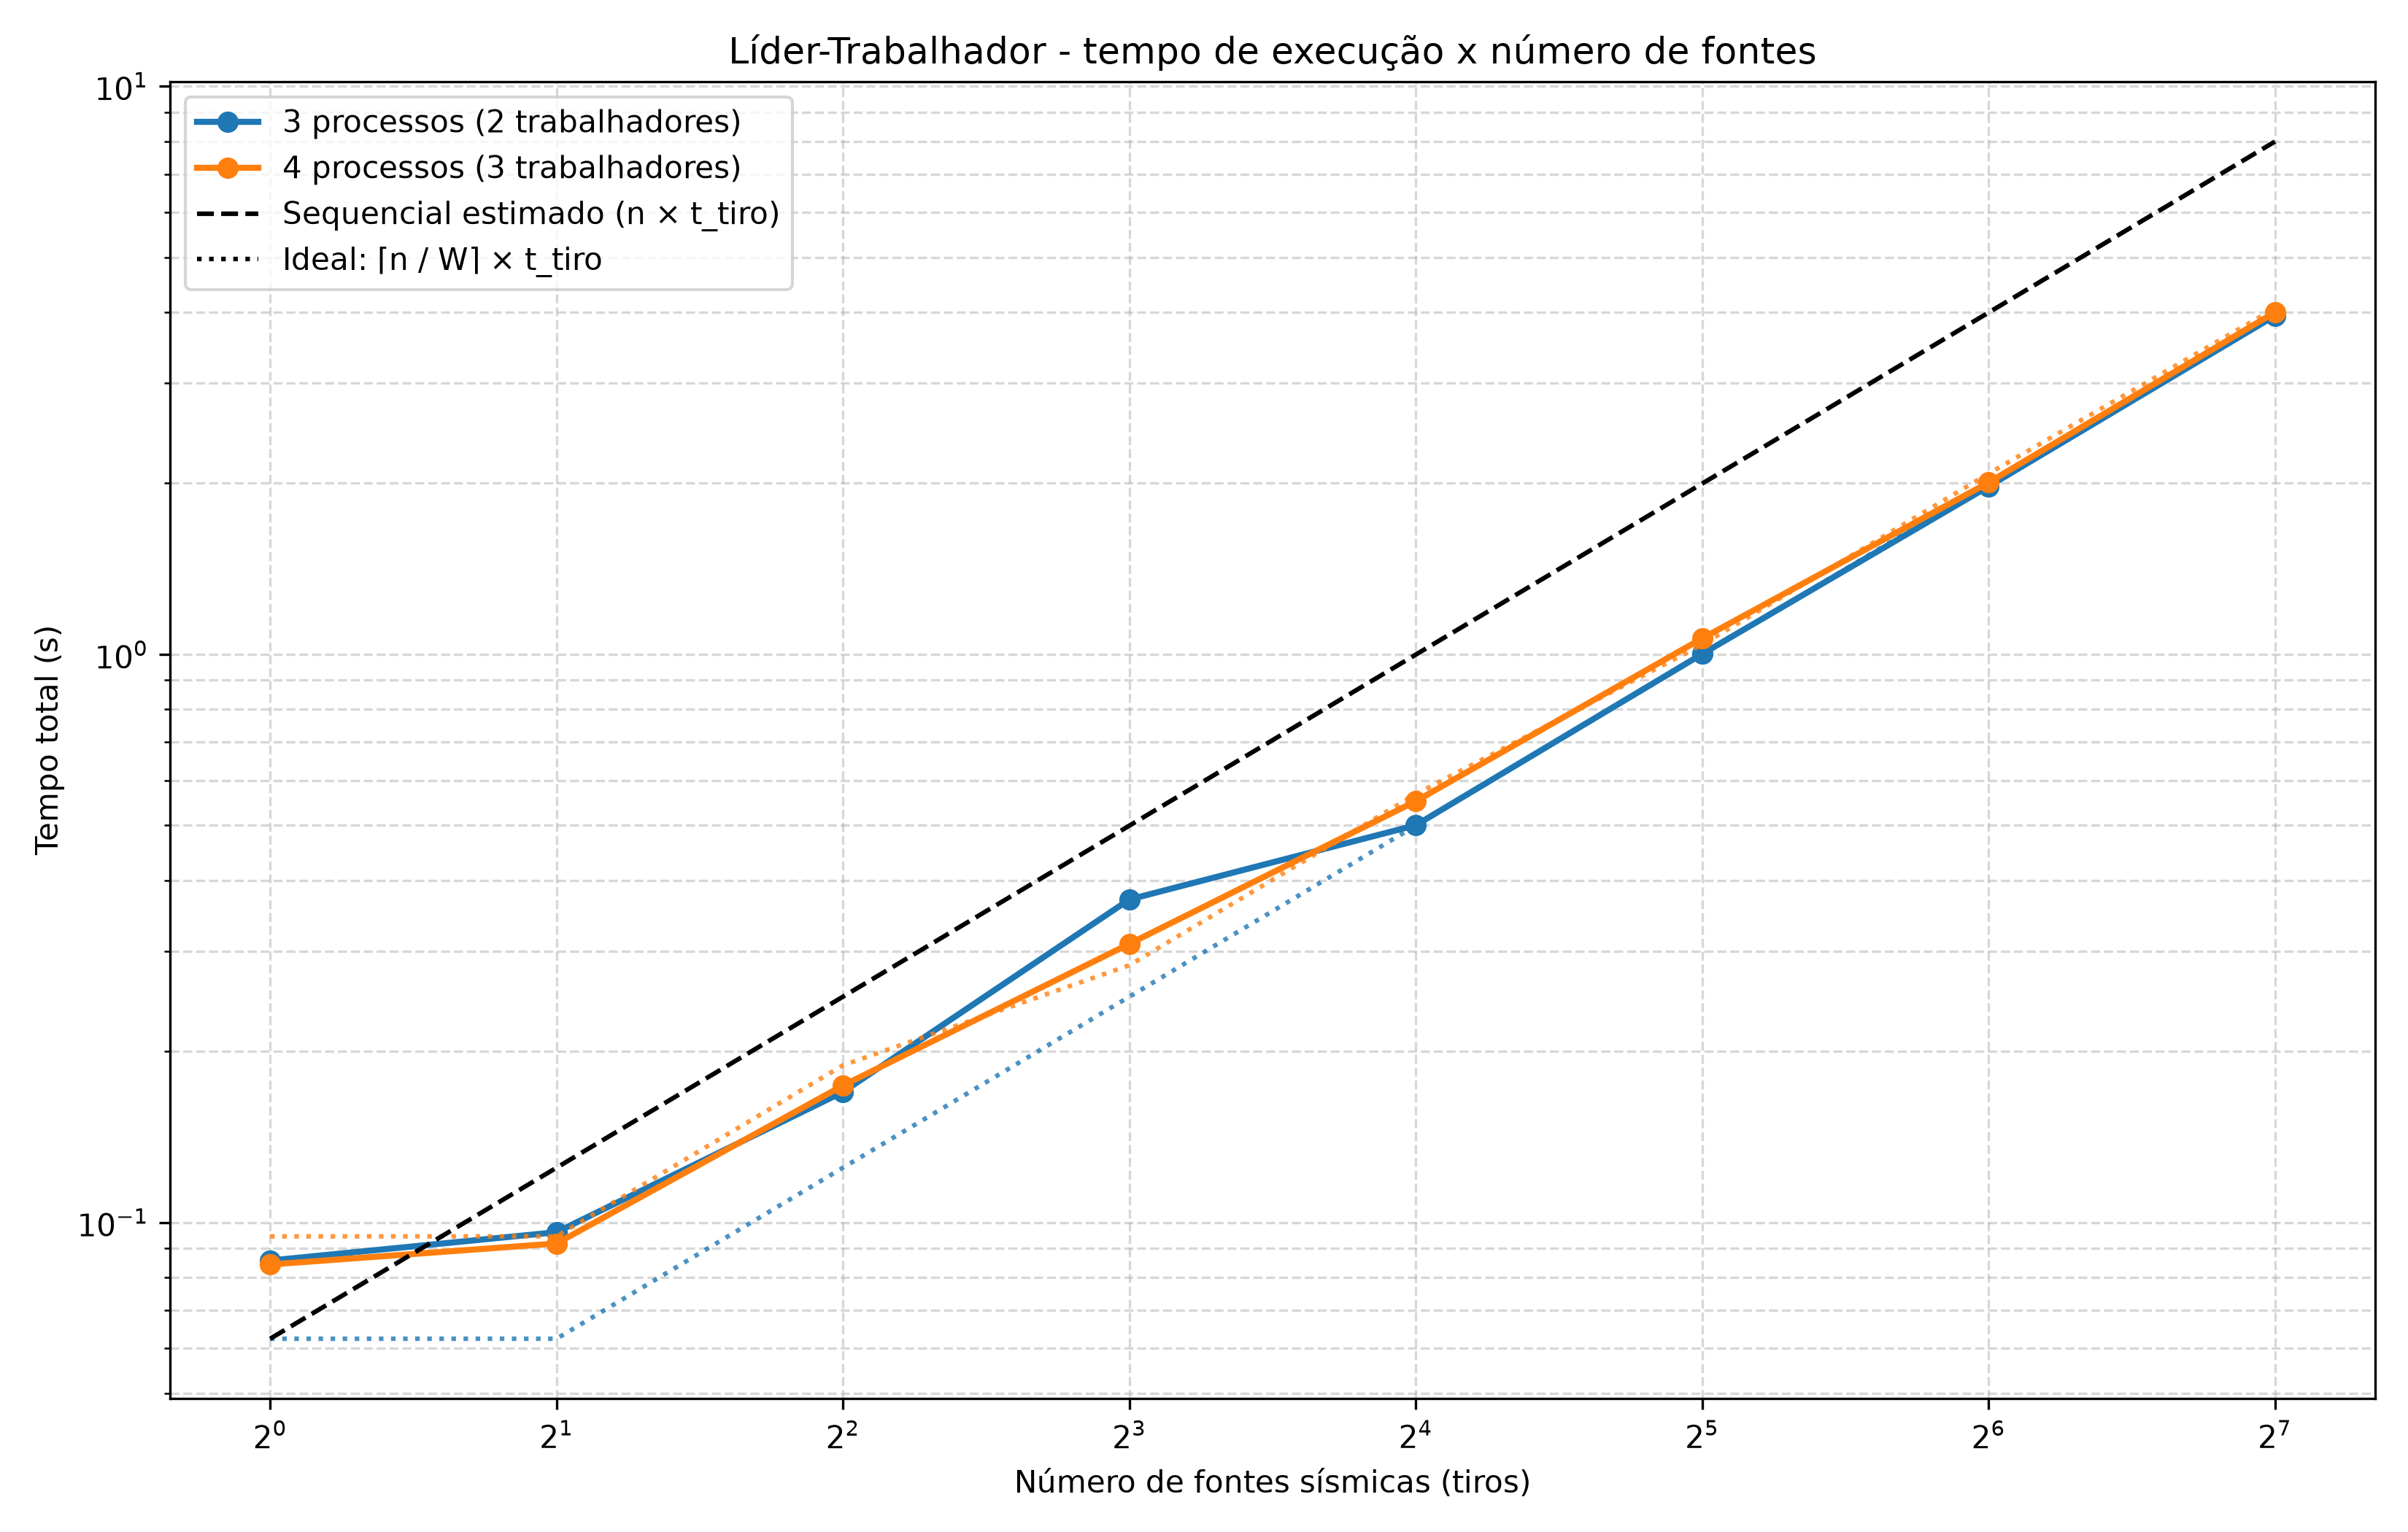
\includegraphics[width=\linewidth]{Tarefa18/tarefa18_tempo.png}
	\end{figure}
	\begin{figure}[H]
		\centering
		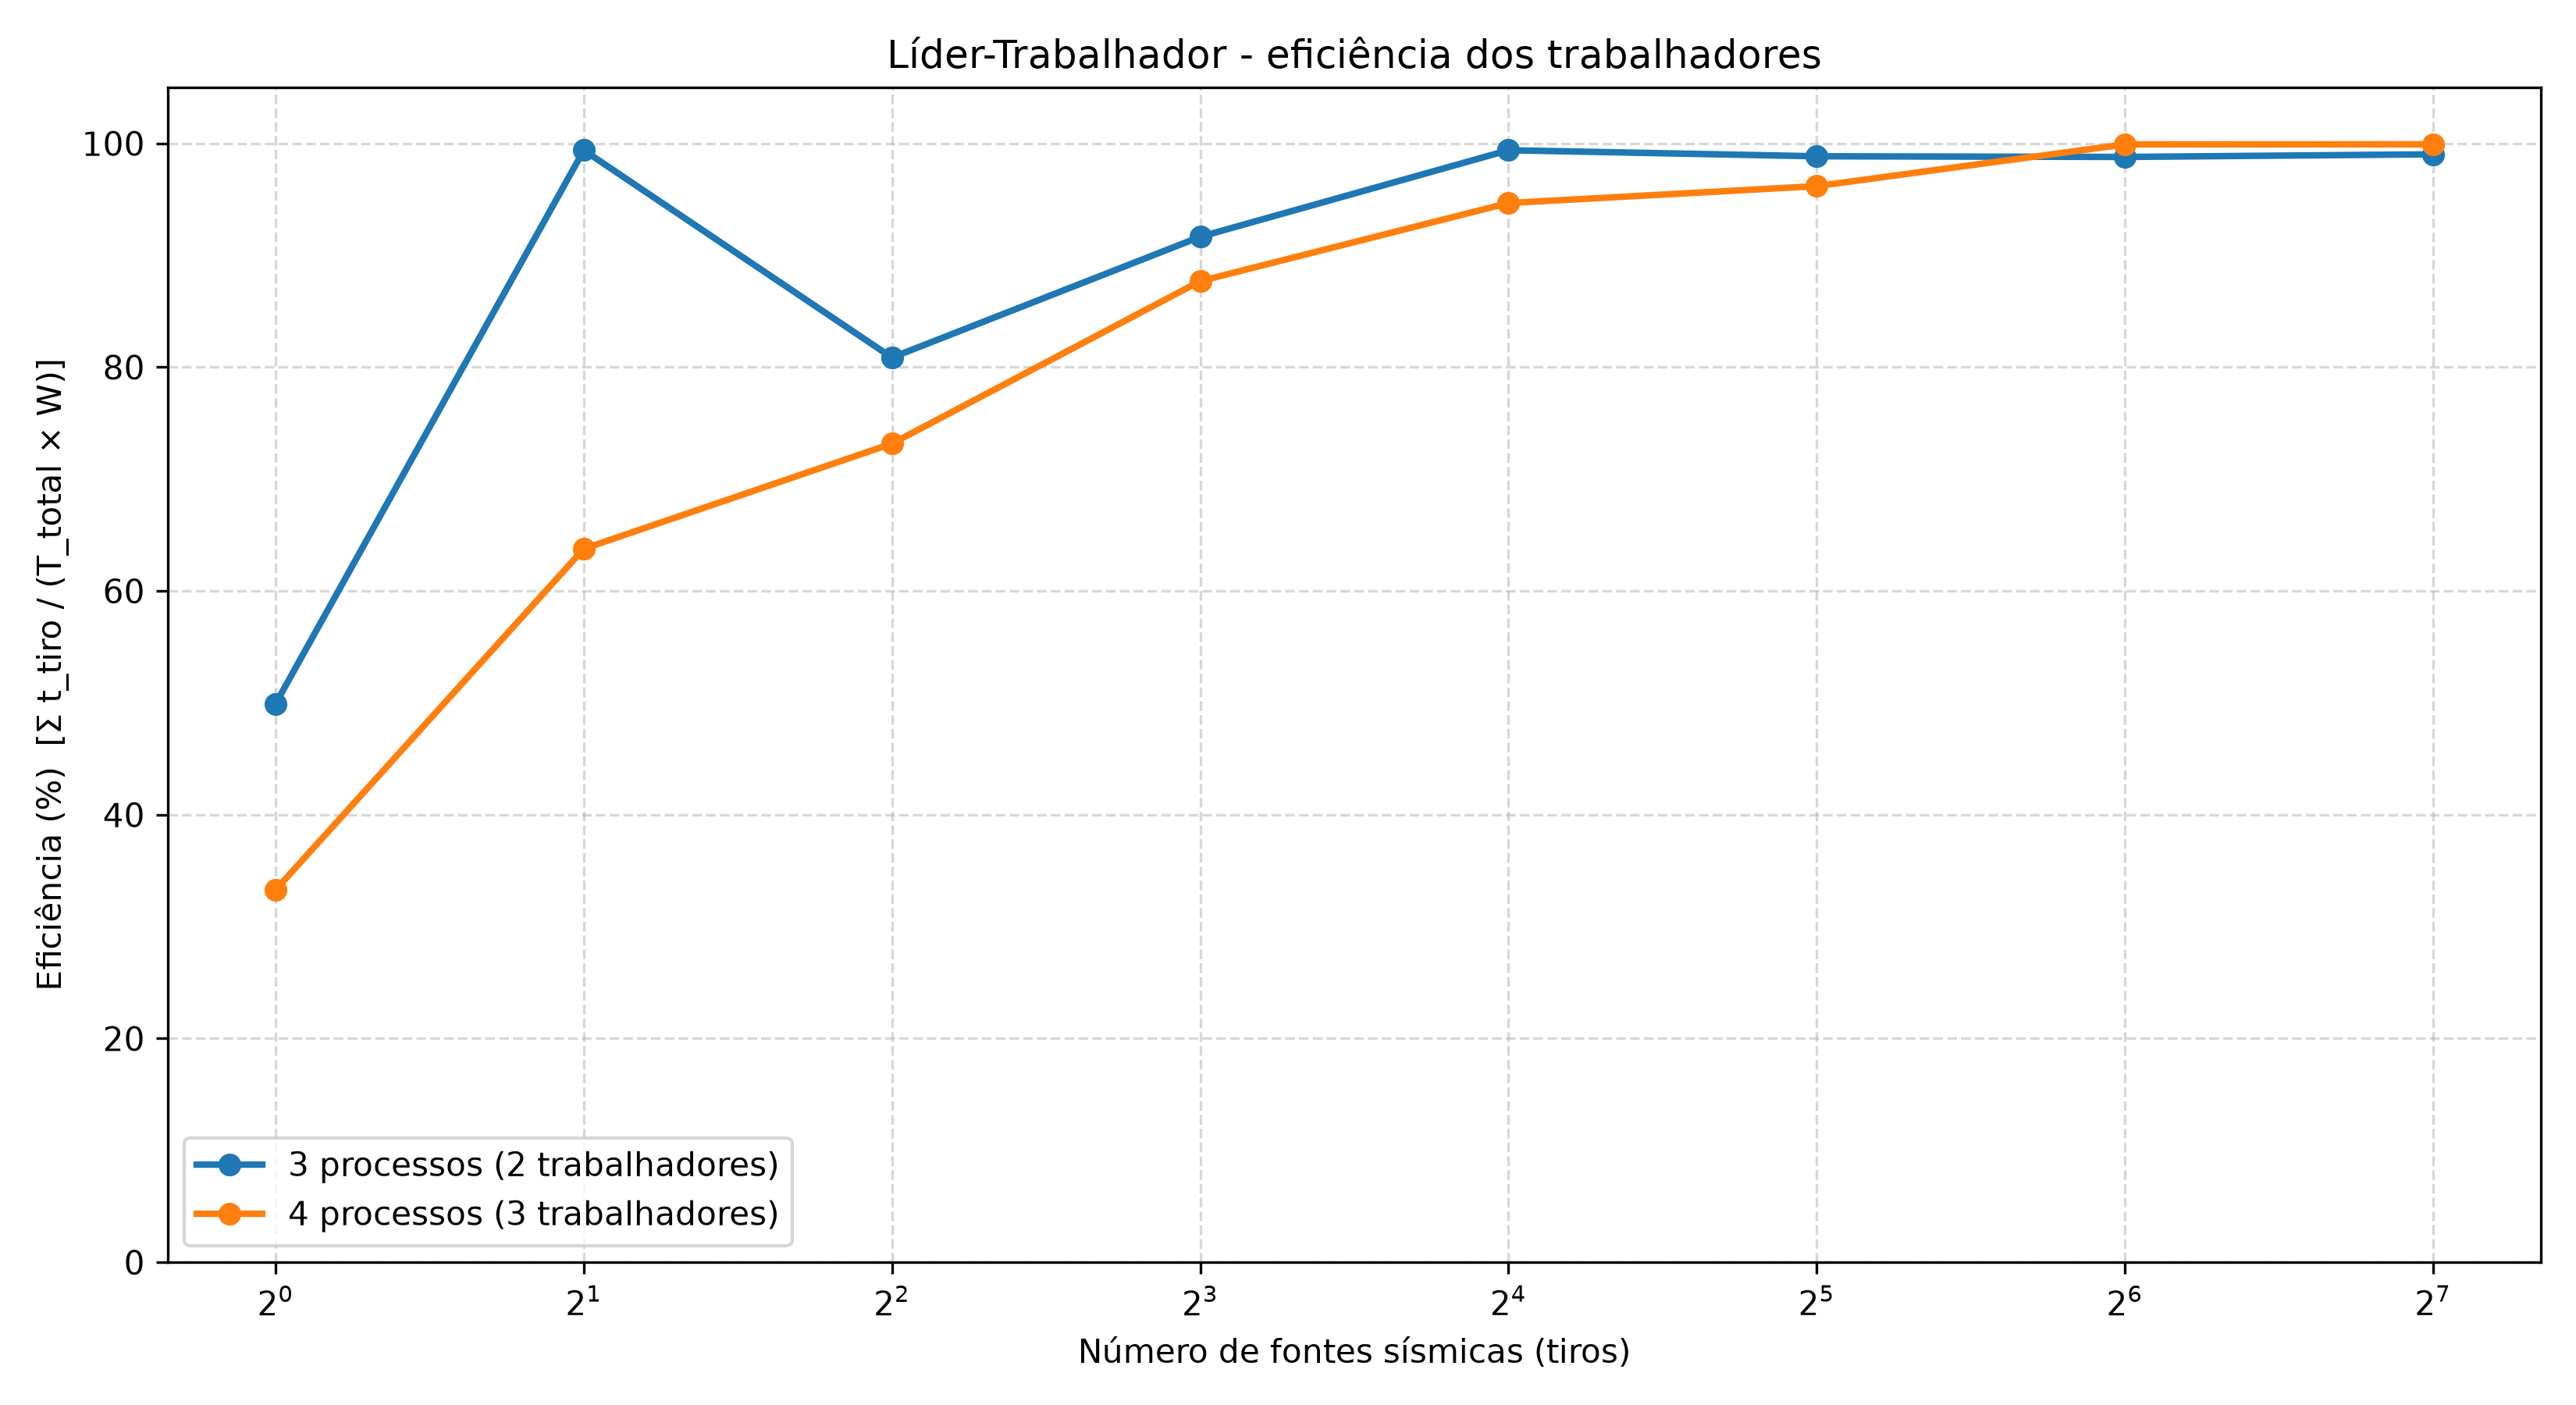
\includegraphics[width=\linewidth]{Tarefa18/tarefa18_eficiencia.png}
	\end{figure}
	\begin{figure}[H]
		\centering
		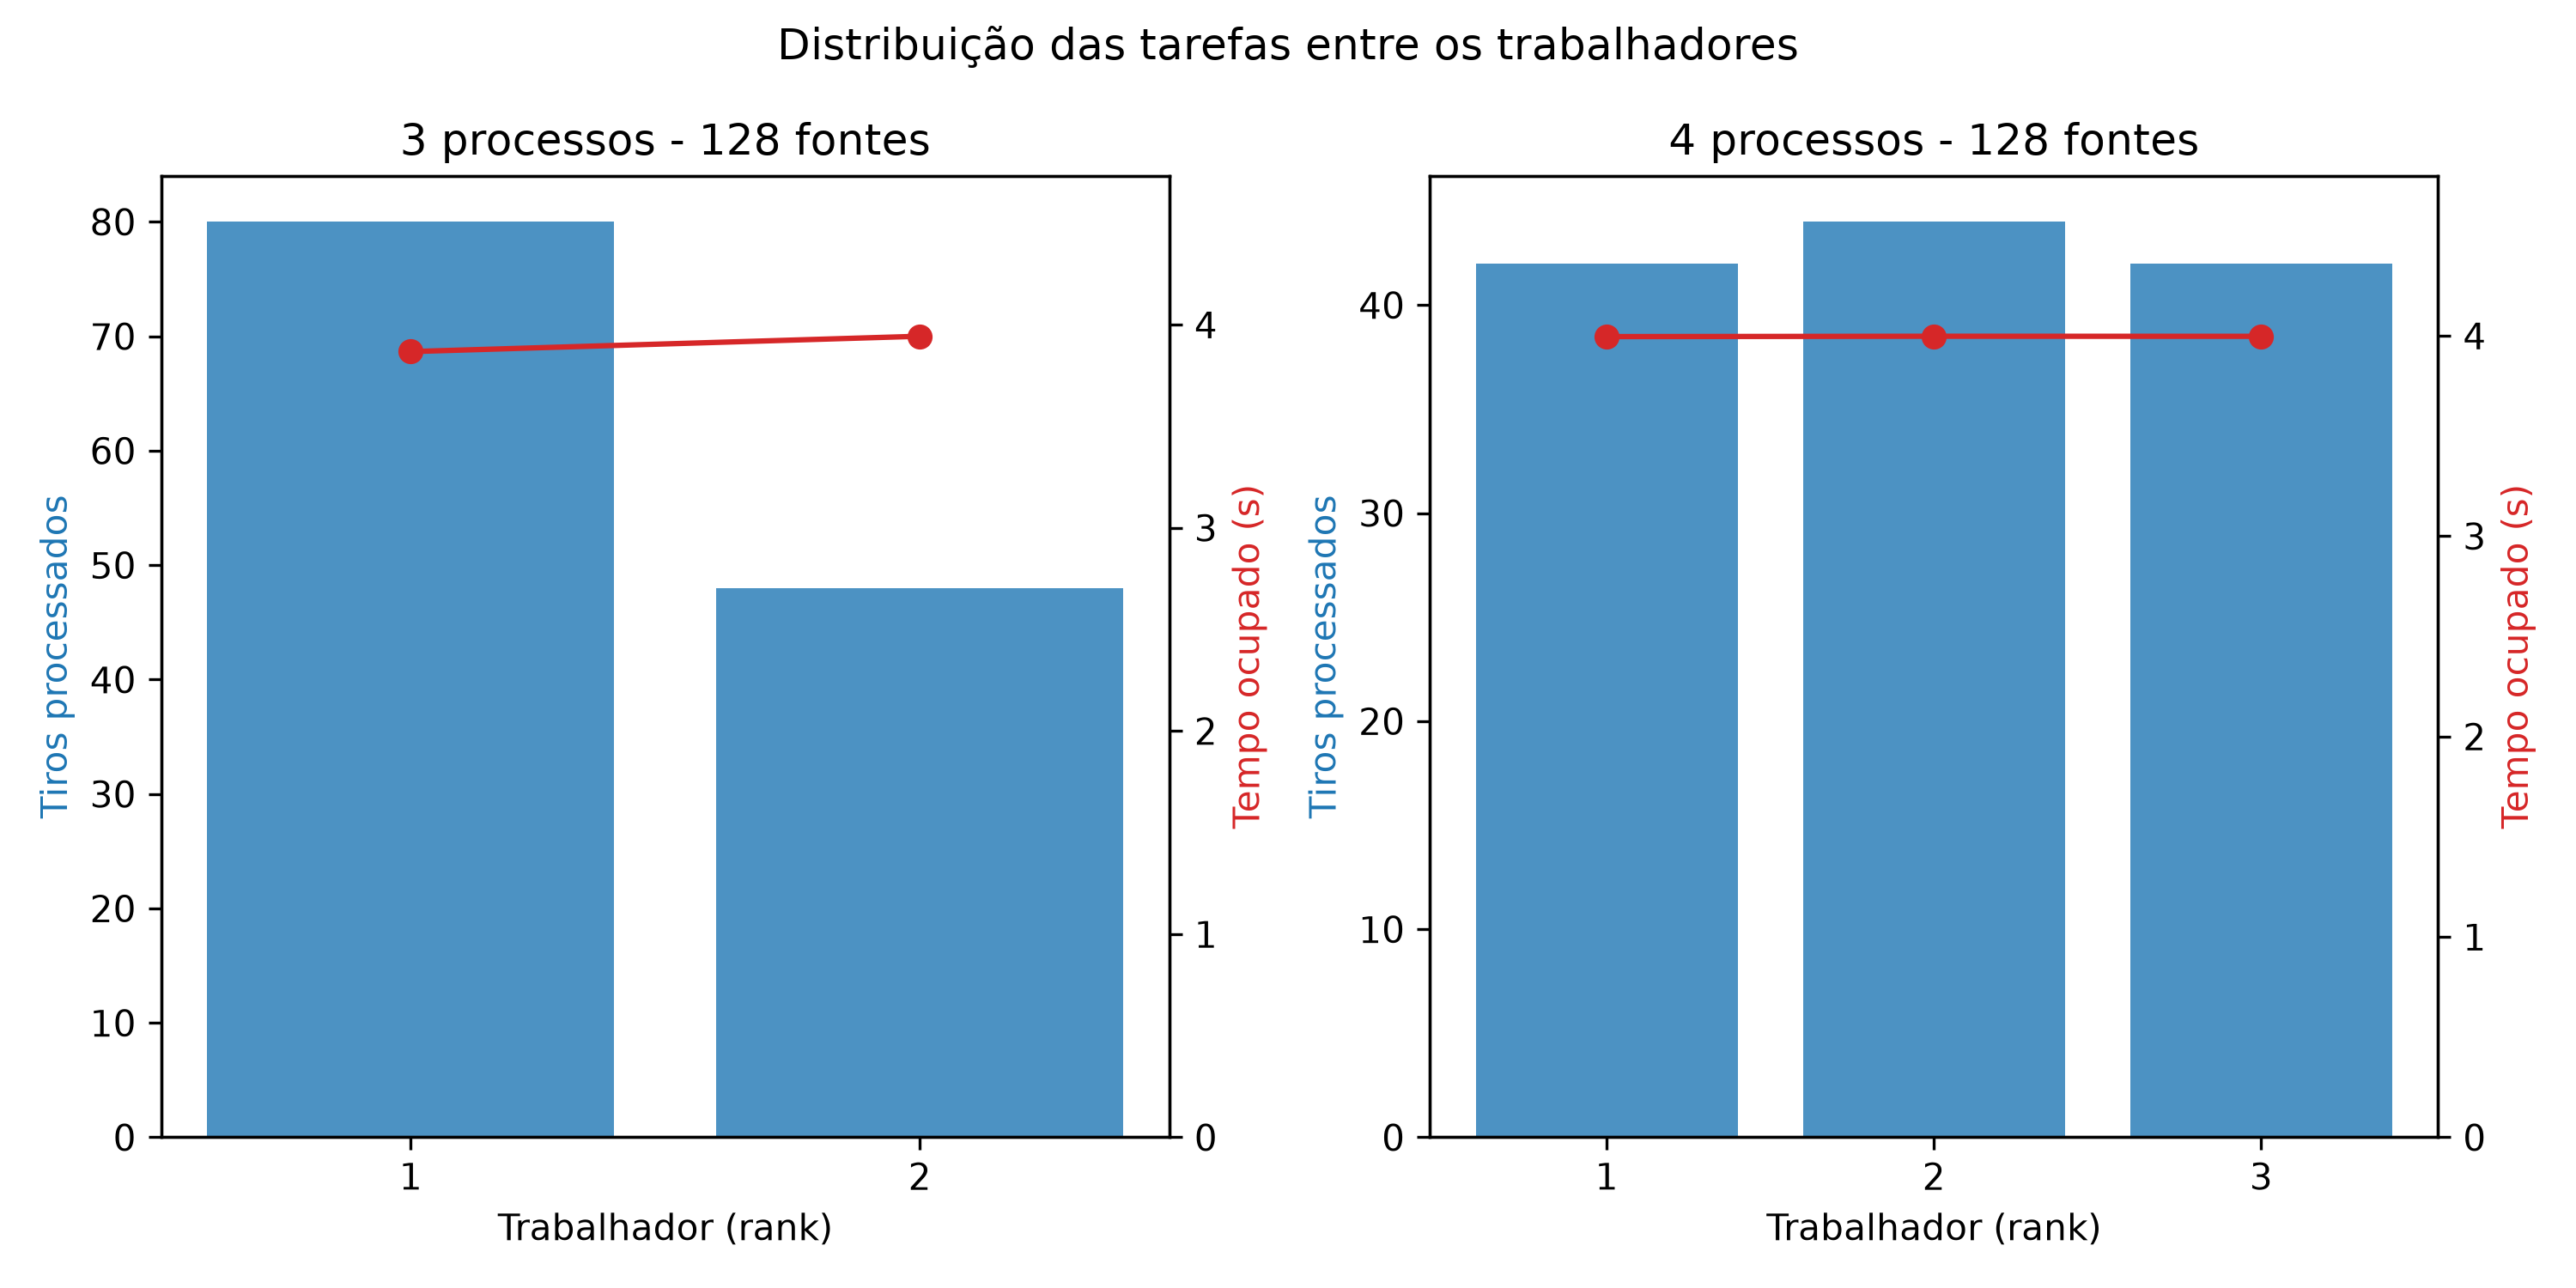
\includegraphics[width=\linewidth]{Tarefa18/tarefa18_distribuicao.png}
	\end{figure}
	\begin{figure}[H]
		\centering
		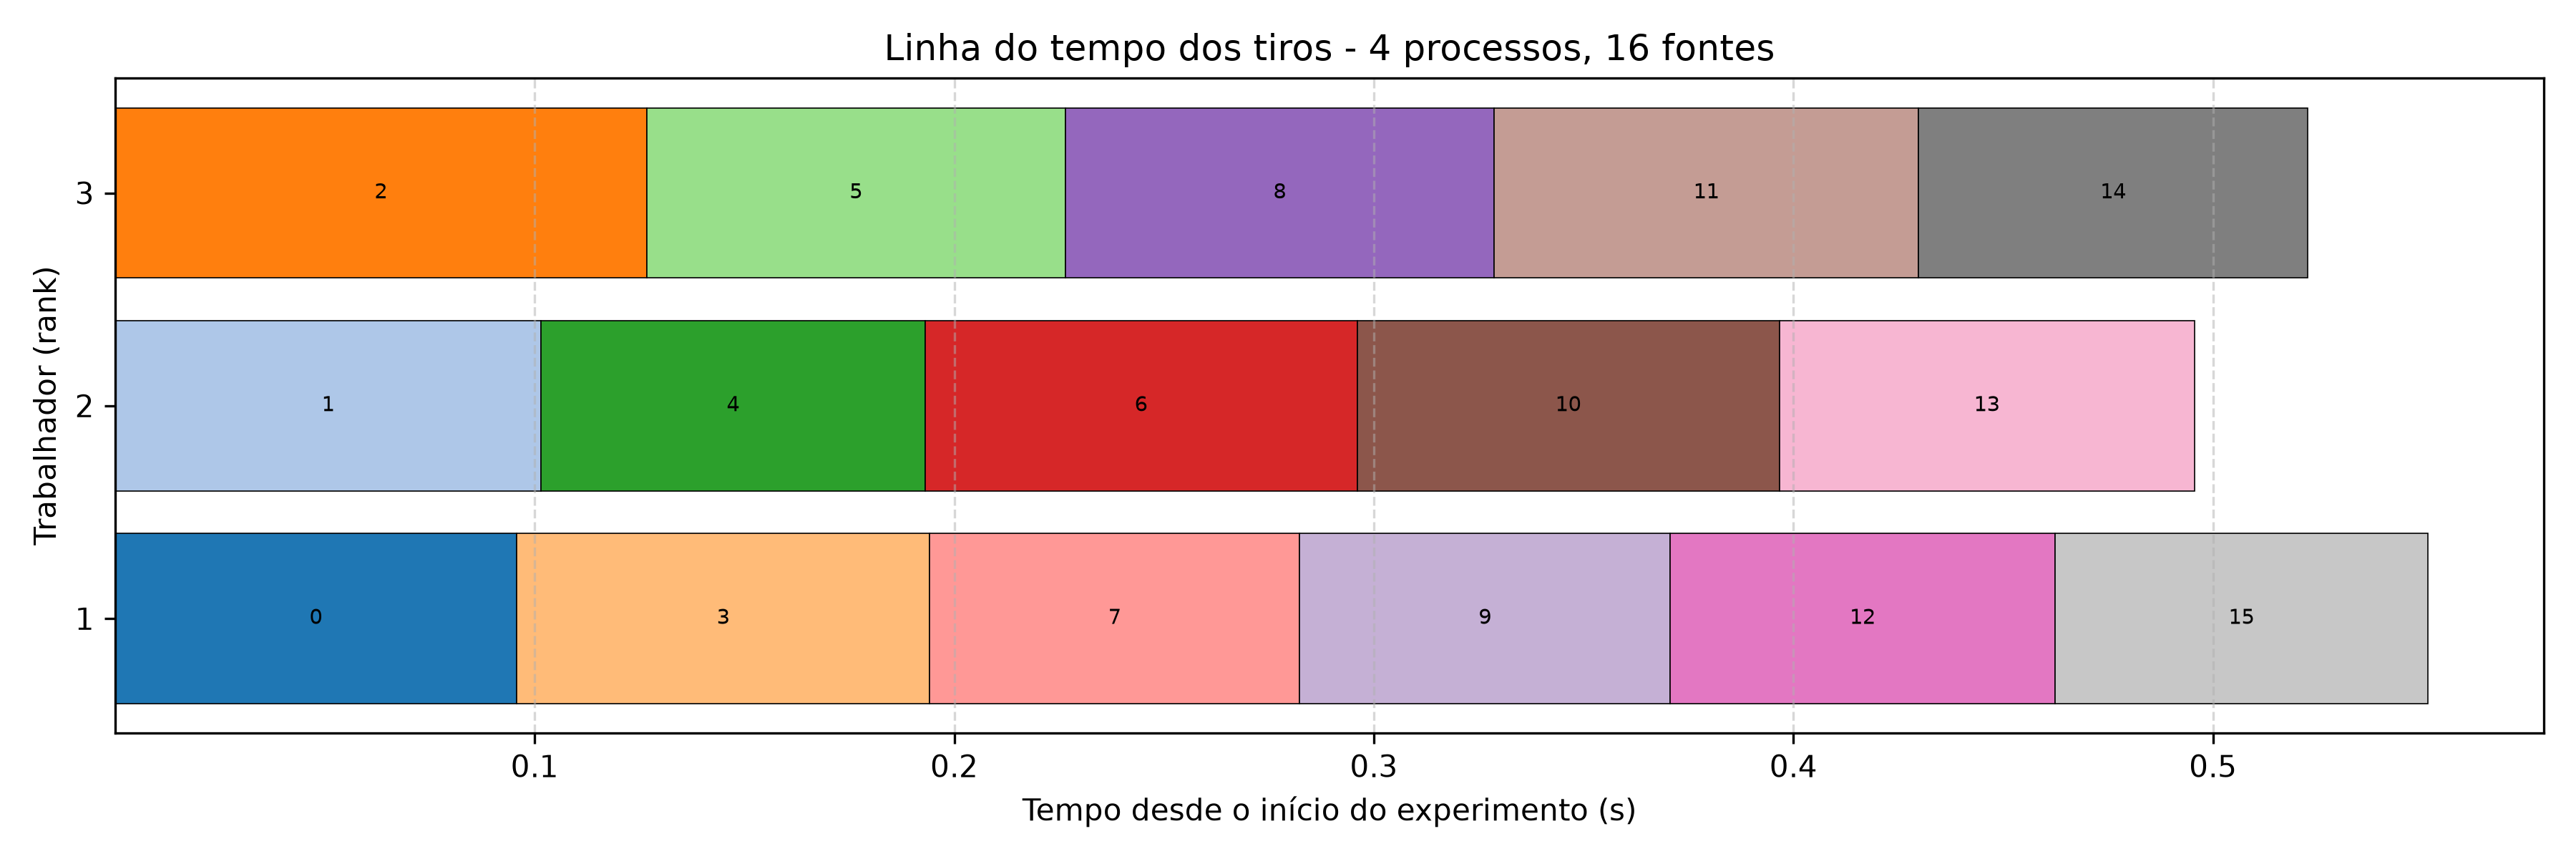
\includegraphics[width=\linewidth]{Tarefa18/tarefa18_gantt.png}
	\end{figure}
	\par{
		O líder envia a cada trabalhador uma struct com a posição da fonte, e assim que um trabalhador termina, recebe uma nova tarefa. Os testes foram feitos com 2 e 3 trabalhadores, de 1 a 128 fontes.
		
		Com poucas fontes, alguns trabalhadores ficam ociosos, mas com muitas fontes o tempo cresce de forma linear e a eficiência chega a 99\%. Com 2 trabalhadores, um processou 80 tiros e o outro 48, mas os dois ficaram ocupados o mesmo tempo, mostrando que o escalonador dinâmico compensa trabalhadores mais lentos. Com 3 trabalhadores não houve ganho, pois o computador usado tem apenas 2 núcleos físicos.
		
		Para evitar deadlock, o trabalhador sempre recebe antes de enviar, e o líder só envia uma nova tarefa depois de receber o resultado anterior, recebendo de qualquer trabalhador e usando tags diferentes para tarefa, resultado e encerramento.
	}
	\subsection{\subtTres}
	\begin{lstlisting}[language=c, title=main.c]
#include <math.h>
#include <mpi.h>
#include <stddef.h>
#include <stdio.h>
#include <stdlib.h>
#include <string.h>

#define NX 200
#define NZ 100

#define DX 10.0
#define DZ 10.0

#define DT 0.001
#define NT 1000

#define VELOCIDADE 2000.0

#define SZ 50
#define RZ 5

#define PI 3.14159265358979323846

#define LIDER 0

#define MAX_SISMOGRAMAS_SALVOS 16

#define TAG_TAREFA 1
#define TAG_RESULTADO 2
#define TAG_FIM 3

static const size_t quantidades_fontes[] = {1, 2, 4, 8, 16, 32, 64, 128};
static const size_t total_experimentos =
    sizeof(quantidades_fontes) / sizeof(quantidades_fontes[0]);

typedef struct {
    int id;
    int sx;
    int sz;
} Tiro;

typedef struct {
    int id;
    int trabalhador;
    double tempo_s;
    double amp_max;
} Resultado;

static MPI_Datatype cria_tipo_tiro(void)
{
    int blocos[3] = {1, 1, 1};
    MPI_Aint deslocamentos[3] = {offsetof(Tiro, id), offsetof(Tiro, sx),
                                 offsetof(Tiro, sz)};
    MPI_Datatype tipos[3] = {MPI_INT, MPI_INT, MPI_INT};

    MPI_Datatype tmp, tipo;
    MPI_Type_create_struct(3, blocos, deslocamentos, tipos, &tmp);

    MPI_Type_create_resized(tmp, 0, sizeof(Tiro), &tipo);
    MPI_Type_commit(&tipo);
    MPI_Type_free(&tmp);
    return tipo;
}

static MPI_Datatype cria_tipo_resultado(void)
{
    int blocos[4] = {1, 1, 1, 1};
    MPI_Aint deslocamentos[4] = {
        offsetof(Resultado, id), offsetof(Resultado, trabalhador),
        offsetof(Resultado, tempo_s), offsetof(Resultado, amp_max)};
    MPI_Datatype tipos[4] = {MPI_INT, MPI_INT, MPI_DOUBLE, MPI_DOUBLE};

    MPI_Datatype tmp, tipo;
    MPI_Type_create_struct(4, blocos, deslocamentos, tipos, &tmp);
    MPI_Type_create_resized(tmp, 0, sizeof(Resultado), &tipo);
    MPI_Type_commit(&tipo);
    MPI_Type_free(&tmp);
    return tipo;
}

static double ricker(double t, double f0)
{
    double t0 = 1.0 / f0;
    double x = PI * f0 * (t - t0);
    return (1.0 - 2.0 * x * x) * exp(-x * x);
}

static void inicializa_modelo(double *vel)
{
    for (int iz = 0; iz < NZ; iz++)
        for (int ix = 0; ix < NX; ix++)
            vel[iz * NX + ix] = VELOCIDADE;
}

static double processa_tiro(const Tiro *tiro, double *vel, double *u,
                            double *u_old, double *u_new, float *sismograma)
{
    memset(u, 0, NX * NZ * sizeof(double));
    memset(u_old, 0, NX * NZ * sizeof(double));
    memset(u_new, 0, NX * NZ * sizeof(double));

    double f0 = 20.0;
    double dt2 = DT * DT;
    double amp_max = 0.0;
    int source_id = tiro->sz * NX + tiro->sx;

    for (int it = 0; it < NT; it++) {
        double t = it * DT;

        for (int iz = 1; iz < NZ - 1; iz++) {
            for (int ix = 1; ix < NX - 1; ix++) {
                int id = iz * NX + ix;

                double d2udx2 =
                    (u[id + 1] - 2.0 * u[id] + u[id - 1]) / (DX * DX);
                double d2udz2 =
                    (u[id + NX] - 2.0 * u[id] + u[id - NX]) / (DZ * DZ);

                u_new[id] = 2.0 * u[id] - u_old[id] +
                            vel[id] * vel[id] * dt2 * (d2udx2 + d2udz2);
            }
        }

        u_new[source_id] += ricker(t, f0);

        for (int ix = 0; ix < NX; ix++) {
            double a = u_new[RZ * NX + ix];
            sismograma[(size_t)it * NX + ix] = (float)a;
            if (fabs(a) > amp_max) amp_max = fabs(a);
        }

        double *tmp = u_old;
        u_old = u;
        u = u_new;
        u_new = tmp;
    }

    if (tiro->id >= MAX_SISMOGRAMAS_SALVOS) return amp_max;

    char nome[128];
    snprintf(nome, sizeof(nome), "outputs/sismograma_tiro_%03d.bin", tiro->id);
    FILE *fp = fopen(nome, "wb");
    if (fp != NULL) {
        fwrite(sismograma, sizeof(float), (size_t)NT * NX, fp);
        fclose(fp);
    }

    return amp_max;
}

static void trabalhador(int rank, MPI_Datatype tipo_tiro,
                        MPI_Datatype tipo_resultado)
{
    double *vel = malloc(NX * NZ * sizeof(double));
    double *u = malloc(NX * NZ * sizeof(double));
    double *u_old = malloc(NX * NZ * sizeof(double));
    double *u_new = malloc(NX * NZ * sizeof(double));
    float *sismograma = malloc((size_t)NT * NX * sizeof(float));

    if (!vel || !u || !u_old || !u_new || !sismograma) {
        fprintf(stderr, "[%d] Erro de alocacao de memoria\n", rank);
        MPI_Abort(MPI_COMM_WORLD, 1);
    }

    inicializa_modelo(vel);

    while (1) {
        Tiro tiro;
        MPI_Status status;

        MPI_Recv(&tiro, 1, tipo_tiro, LIDER, MPI_ANY_TAG, MPI_COMM_WORLD,
                 &status);

        if (status.MPI_TAG == TAG_FIM) break;

        double ini = MPI_Wtime();
        double amp = processa_tiro(&tiro, vel, u, u_old, u_new, sismograma);
        double fim = MPI_Wtime();

        Resultado r = {tiro.id, rank, fim - ini, amp};
        MPI_Send(&r, 1, tipo_resultado, LIDER, TAG_RESULTADO, MPI_COMM_WORLD);
    }

    free(vel);
    free(u);
    free(u_old);
    free(u_new);
    free(sismograma);
}

typedef struct {
    int trabalhador;
    double inicio_s;
    double fim_s;
    double tempo_s;
    double amp_max;
} RegistroTiro;

static Tiro monta_tiro(int id, int n_fontes)
{
    Tiro t;
    t.id = id;

    t.sx = n_fontes == 1 ? NX / 2 : 10 + id * (NX - 21) / (n_fontes - 1);
    t.sz = SZ;
    return t;
}

static void lider_experimento(int n_fontes, int processos,
                              MPI_Datatype tipo_tiro,
                              MPI_Datatype tipo_resultado, FILE *json,
                              int ultimo)
{
    int trabalhadores = processos - 1;
    RegistroTiro *registros = calloc(n_fontes, sizeof(RegistroTiro));
    int *tarefas = calloc(processos, sizeof(int));
    double *ocupado = calloc(processos, sizeof(double));

    int proximo = 0;
    int ativos = 0;

    double t0 = MPI_Wtime();

    for (int w = 1; w <= trabalhadores && proximo < n_fontes; w++) {
        Tiro tiro = monta_tiro(proximo, n_fontes);
        registros[proximo].trabalhador = w;
        registros[proximo].inicio_s = MPI_Wtime() - t0;
        MPI_Send(&tiro, 1, tipo_tiro, w, TAG_TAREFA, MPI_COMM_WORLD);
        proximo++;
        ativos++;
    }

    while (ativos > 0) {
        Resultado r;
        MPI_Status status;
        MPI_Recv(&r, 1, tipo_resultado, MPI_ANY_SOURCE, TAG_RESULTADO,
                 MPI_COMM_WORLD, &status);

        int w = status.MPI_SOURCE;
        registros[r.id].fim_s = MPI_Wtime() - t0;
        registros[r.id].tempo_s = r.tempo_s;
        registros[r.id].amp_max = r.amp_max;
        tarefas[w]++;
        ocupado[w] += r.tempo_s;

        if (proximo < n_fontes) {
            Tiro tiro = monta_tiro(proximo, n_fontes);
            registros[proximo].trabalhador = w;
            registros[proximo].inicio_s = MPI_Wtime() - t0;
            MPI_Send(&tiro, 1, tipo_tiro, w, TAG_TAREFA, MPI_COMM_WORLD);
            proximo++;
        } else {
            ativos--;
        }
    }

    double tempo_total = MPI_Wtime() - t0;

    double soma = 0.0;
    for (int i = 0; i < n_fontes; i++) soma += registros[i].tempo_s;

    double speedup = soma / tempo_total;
    double eficiencia = speedup / trabalhadores;

    printf("Fontes: %3d | tempo total: %8.4f s | soma dos tiros: %8.4f s | "
           "speedup: %5.2f | eficiencia: %5.1f%% | tarefas/trab:",
           n_fontes, tempo_total, soma, speedup, 100.0 * eficiencia);
    for (int w = 1; w <= trabalhadores; w++) printf(" %d", tarefas[w]);
    printf("\n");

    fprintf(json, "    {\n");
    fprintf(json, "      \"n_fontes\": %d,\n", n_fontes);
    fprintf(json, "      \"tempo_total_s\": %f,\n", tempo_total);
    fprintf(json, "      \"soma_tempo_tiros_s\": %f,\n", soma);
    fprintf(json, "      \"tempo_medio_tiro_s\": %f,\n", soma / n_fontes);
    fprintf(json, "      \"speedup\": %f,\n", speedup);
    fprintf(json, "      \"eficiencia\": %f,\n", eficiencia);

    fprintf(json, "      \"tarefas_por_trabalhador\": [");
    for (int w = 1; w <= trabalhadores; w++)
        fprintf(json, "%d%s", tarefas[w], w < trabalhadores ? ", " : "");
    fprintf(json, "],\n");

    fprintf(json, "      \"tempo_ocupado_por_trabalhador_s\": [");
    for (int w = 1; w <= trabalhadores; w++)
        fprintf(json, "%f%s", ocupado[w], w < trabalhadores ? ", " : "");
    fprintf(json, "],\n");

    fprintf(json, "      \"tiros\": [\n");
    for (int i = 0; i < n_fontes; i++) {
        Tiro t = monta_tiro(i, n_fontes);
        fprintf(json,
                "        {\"id\": %d, \"sx\": %d, \"sz\": %d, "
                "\"trabalhador\": %d, \"inicio_s\": %f, \"fim_s\": %f, "
                "\"tempo_s\": %f, \"amp_max\": %g}%s\n",
                i, t.sx, t.sz, registros[i].trabalhador,
                registros[i].inicio_s, registros[i].fim_s,
                registros[i].tempo_s, registros[i].amp_max,
                i + 1 < n_fontes ? "," : "");
    }
    fprintf(json, "      ]\n");
    fprintf(json, "    }%s\n", ultimo ? "" : ",");

    free(registros);
    free(tarefas);
    free(ocupado);
}

int main(int argc, char *argv[])
{
    MPI_Init(&argc, &argv);

    int rank, processos;
    MPI_Comm_rank(MPI_COMM_WORLD, &rank);
    MPI_Comm_size(MPI_COMM_WORLD, &processos);

    if (processos < 3) {
        if (rank == LIDER)
            fprintf(stderr, "Use pelo menos 3 processos "
                            "(1 lider + 2 trabalhadores).\n");
        MPI_Finalize();
        return 1;
    }

    MPI_Datatype tipo_tiro = cria_tipo_tiro();
    MPI_Datatype tipo_resultado = cria_tipo_resultado();

    if (rank == LIDER) {
        char nome[64];
        snprintf(nome, sizeof(nome), "resultados_np%d.json", processos);
        FILE *json = fopen(nome, "w");
        if (json == NULL) {
            fprintf(stderr, "Erro ao abrir %s\n", nome);
            MPI_Abort(MPI_COMM_WORLD, 1);
        }

        printf("Lider-Trabalhador: %d processos (1 lider + %d trabalhadores)\n",
               processos, processos - 1);
        printf("Malha %dx%d, %d passos de tempo por tiro\n\n", NX, NZ, NT);

        fprintf(json, "{\n");
        fprintf(json, "  \"processos\": %d,\n", processos);
        fprintf(json, "  \"trabalhadores\": %d,\n", processos - 1);
        fprintf(json, "  \"nx\": %d, \"nz\": %d, \"nt\": %d,\n", NX, NZ, NT);
        fprintf(json, "  \"experimentos\": [\n");

        for (size_t e = 0; e < total_experimentos; e++) {
            lider_experimento((int)quantidades_fontes[e], processos, tipo_tiro,
                              tipo_resultado, json,
                              e + 1 == total_experimentos);
        }

        fprintf(json, "  ]\n}\n");
        fclose(json);

        Tiro vazio = {-1, 0, 0};
        for (int w = 1; w < processos; w++)
            MPI_Send(&vazio, 1, tipo_tiro, w, TAG_FIM, MPI_COMM_WORLD);

        printf("\nResultados salvos em %s\n", nome);
    } else {
        trabalhador(rank, tipo_tiro, tipo_resultado);
    }

    MPI_Type_free(&tipo_tiro);
    MPI_Type_free(&tipo_resultado);

    MPI_Finalize();
    return 0;
}
\end{lstlisting}
	\begin{lstlisting}[language=bash, title=script\_mpi.sh]
#!/bin/bash
#SBATCH --job-name=MPI_lider_trab_akira
#SBATCH --output=saida%j.out
#SBATCH --error=erro%j.err
#SBATCH --partition=amd-512
#SBATCH --nodes=2
#SBATCH --ntasks-per-node=9
#SBATCH --time=0-0:20

cd "${SLURM_SUBMIT_DIR:-.}"
mkdir -p outputs

MPIRUN_OPTS=""
if mpirun --version 2>&1 | grep -qi "open mpi"; then
    MPIRUN_OPTS="--mca btl ^openib"
fi

echo "===== Build ====="
mpicc -O2 main.c -o outputs/main -lm || exit 1

for np in 3 5 9 17; do
    echo "===== ${np} processos ====="
    mpirun -np ${np} ${MPIRUN_OPTS} ./outputs/main
done

echo "===== Graficos ====="
if command -v python3 > /dev/null 2>&1 && python3 -c "import matplotlib" 2> /dev/null; then
    python3 plot.py
else
    echo "matplotlib indisponivel: copie os resultados_np*.json e rode plot.py localmente."
fi
\end{lstlisting}
	
	\newpage
	\onehalfspacing
	\section{TAREFA 19}
	\subsection{\subtUm}
	\par{Implementar um programa MPI que calcule o produto y=A*x, onde A é uma matriz M*N e x é um vetor de tamanho N.
		
		A matriz deve ser dividida por linhas entre os processos com MPI\_Scatter, o vetor x deve ser distribuído com MPI\_Bcast, e cada processo deve calcular os elementos e enviá-los de volta ao processo 0 com MPI\_Gather.
		
		Comparar os tempos com diferentes tamanhos de matriz e números de processos, executando pelo NPAD com pelo menos dois nós.}
	\subsection{\subtDois}
	\begin{figure}[H]
		\centering
		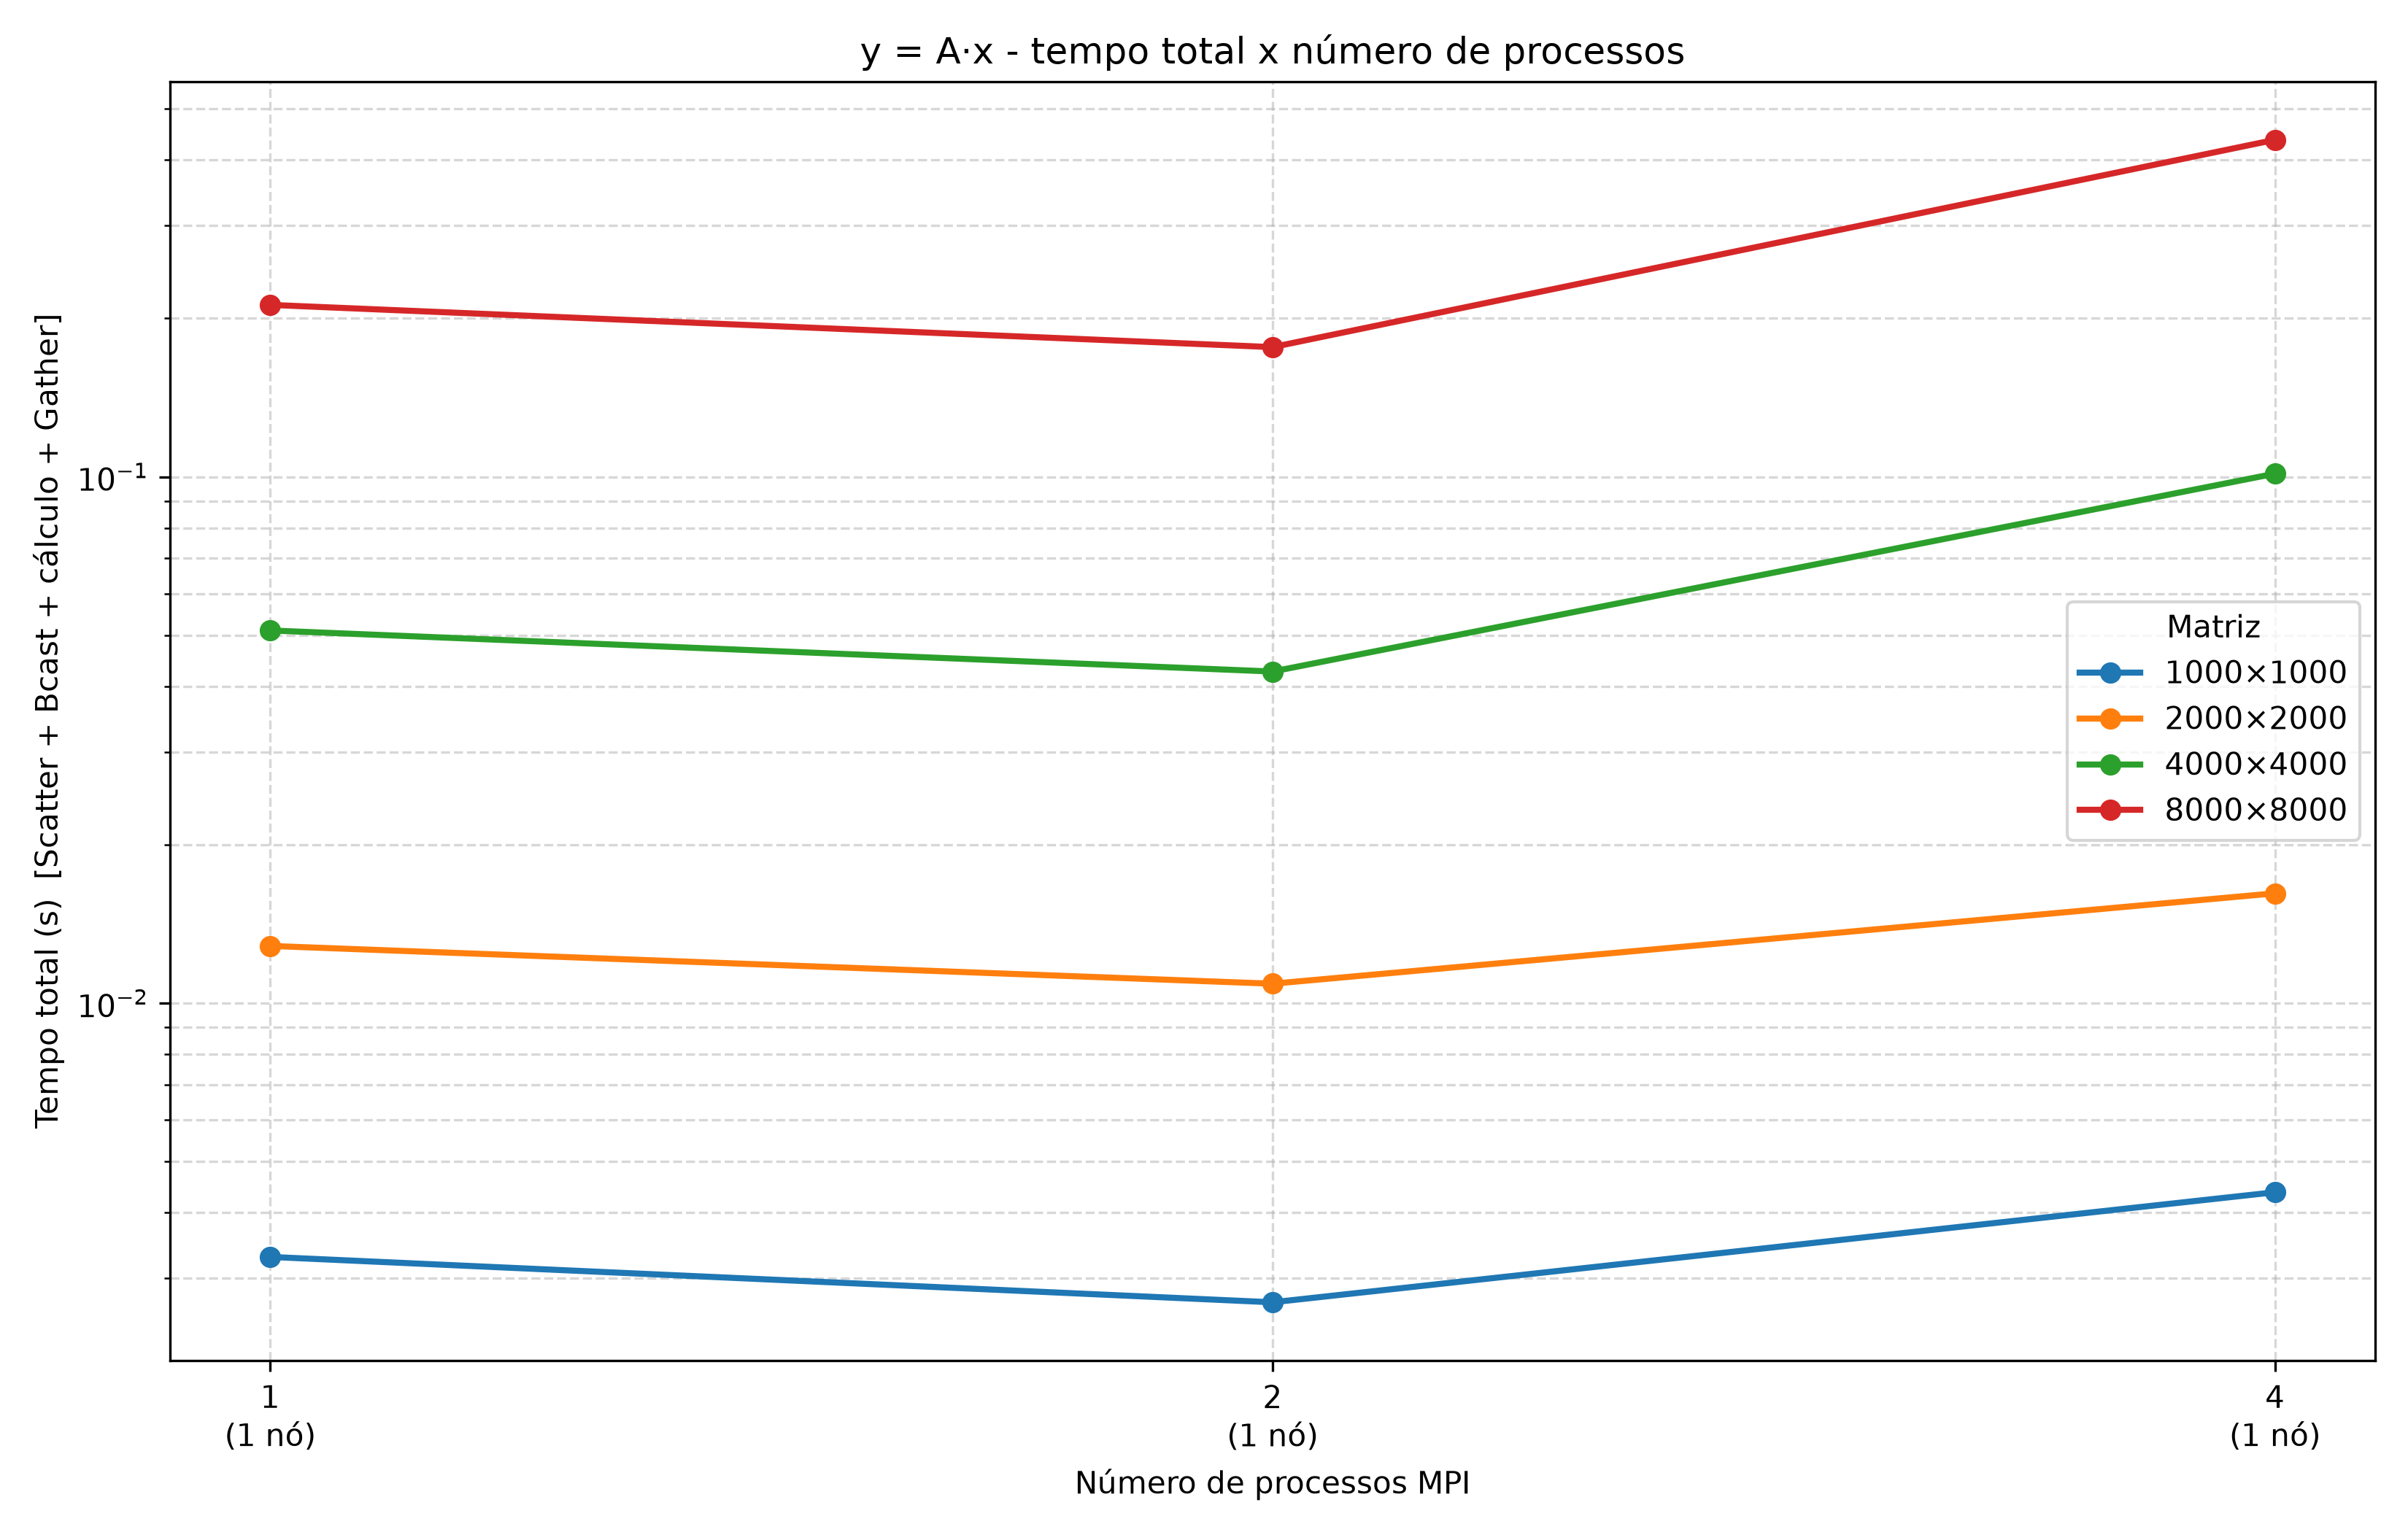
\includegraphics[width=\linewidth]{Tarefa19/tarefa19_tempo.png}
	\end{figure}
	\begin{figure}[H]
		\centering
		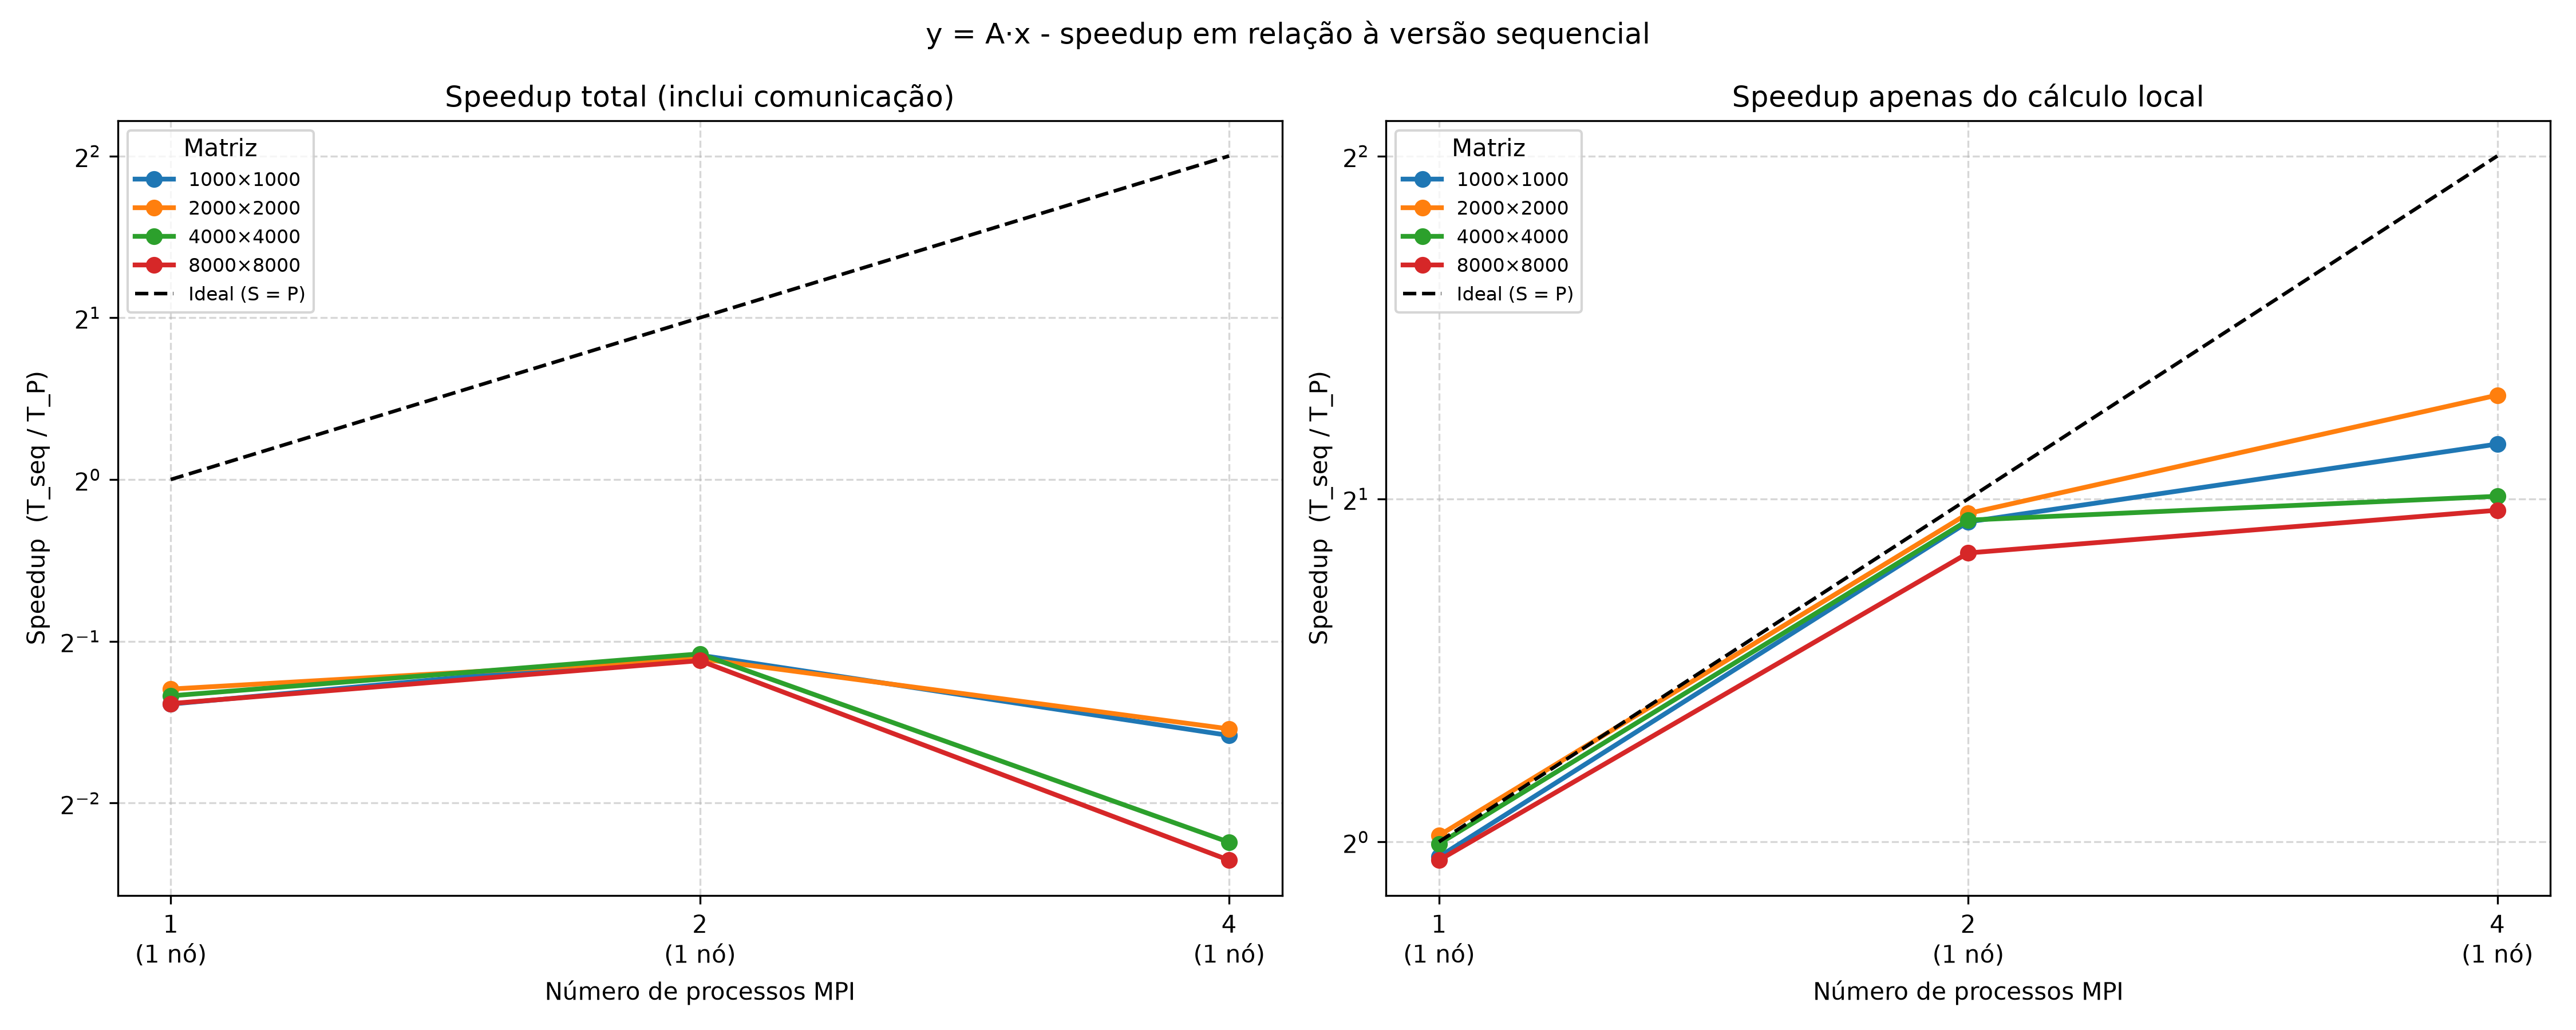
\includegraphics[width=\linewidth]{Tarefa19/tarefa19_speedup.png}
	\end{figure}
	\begin{figure}[H]
		\centering
		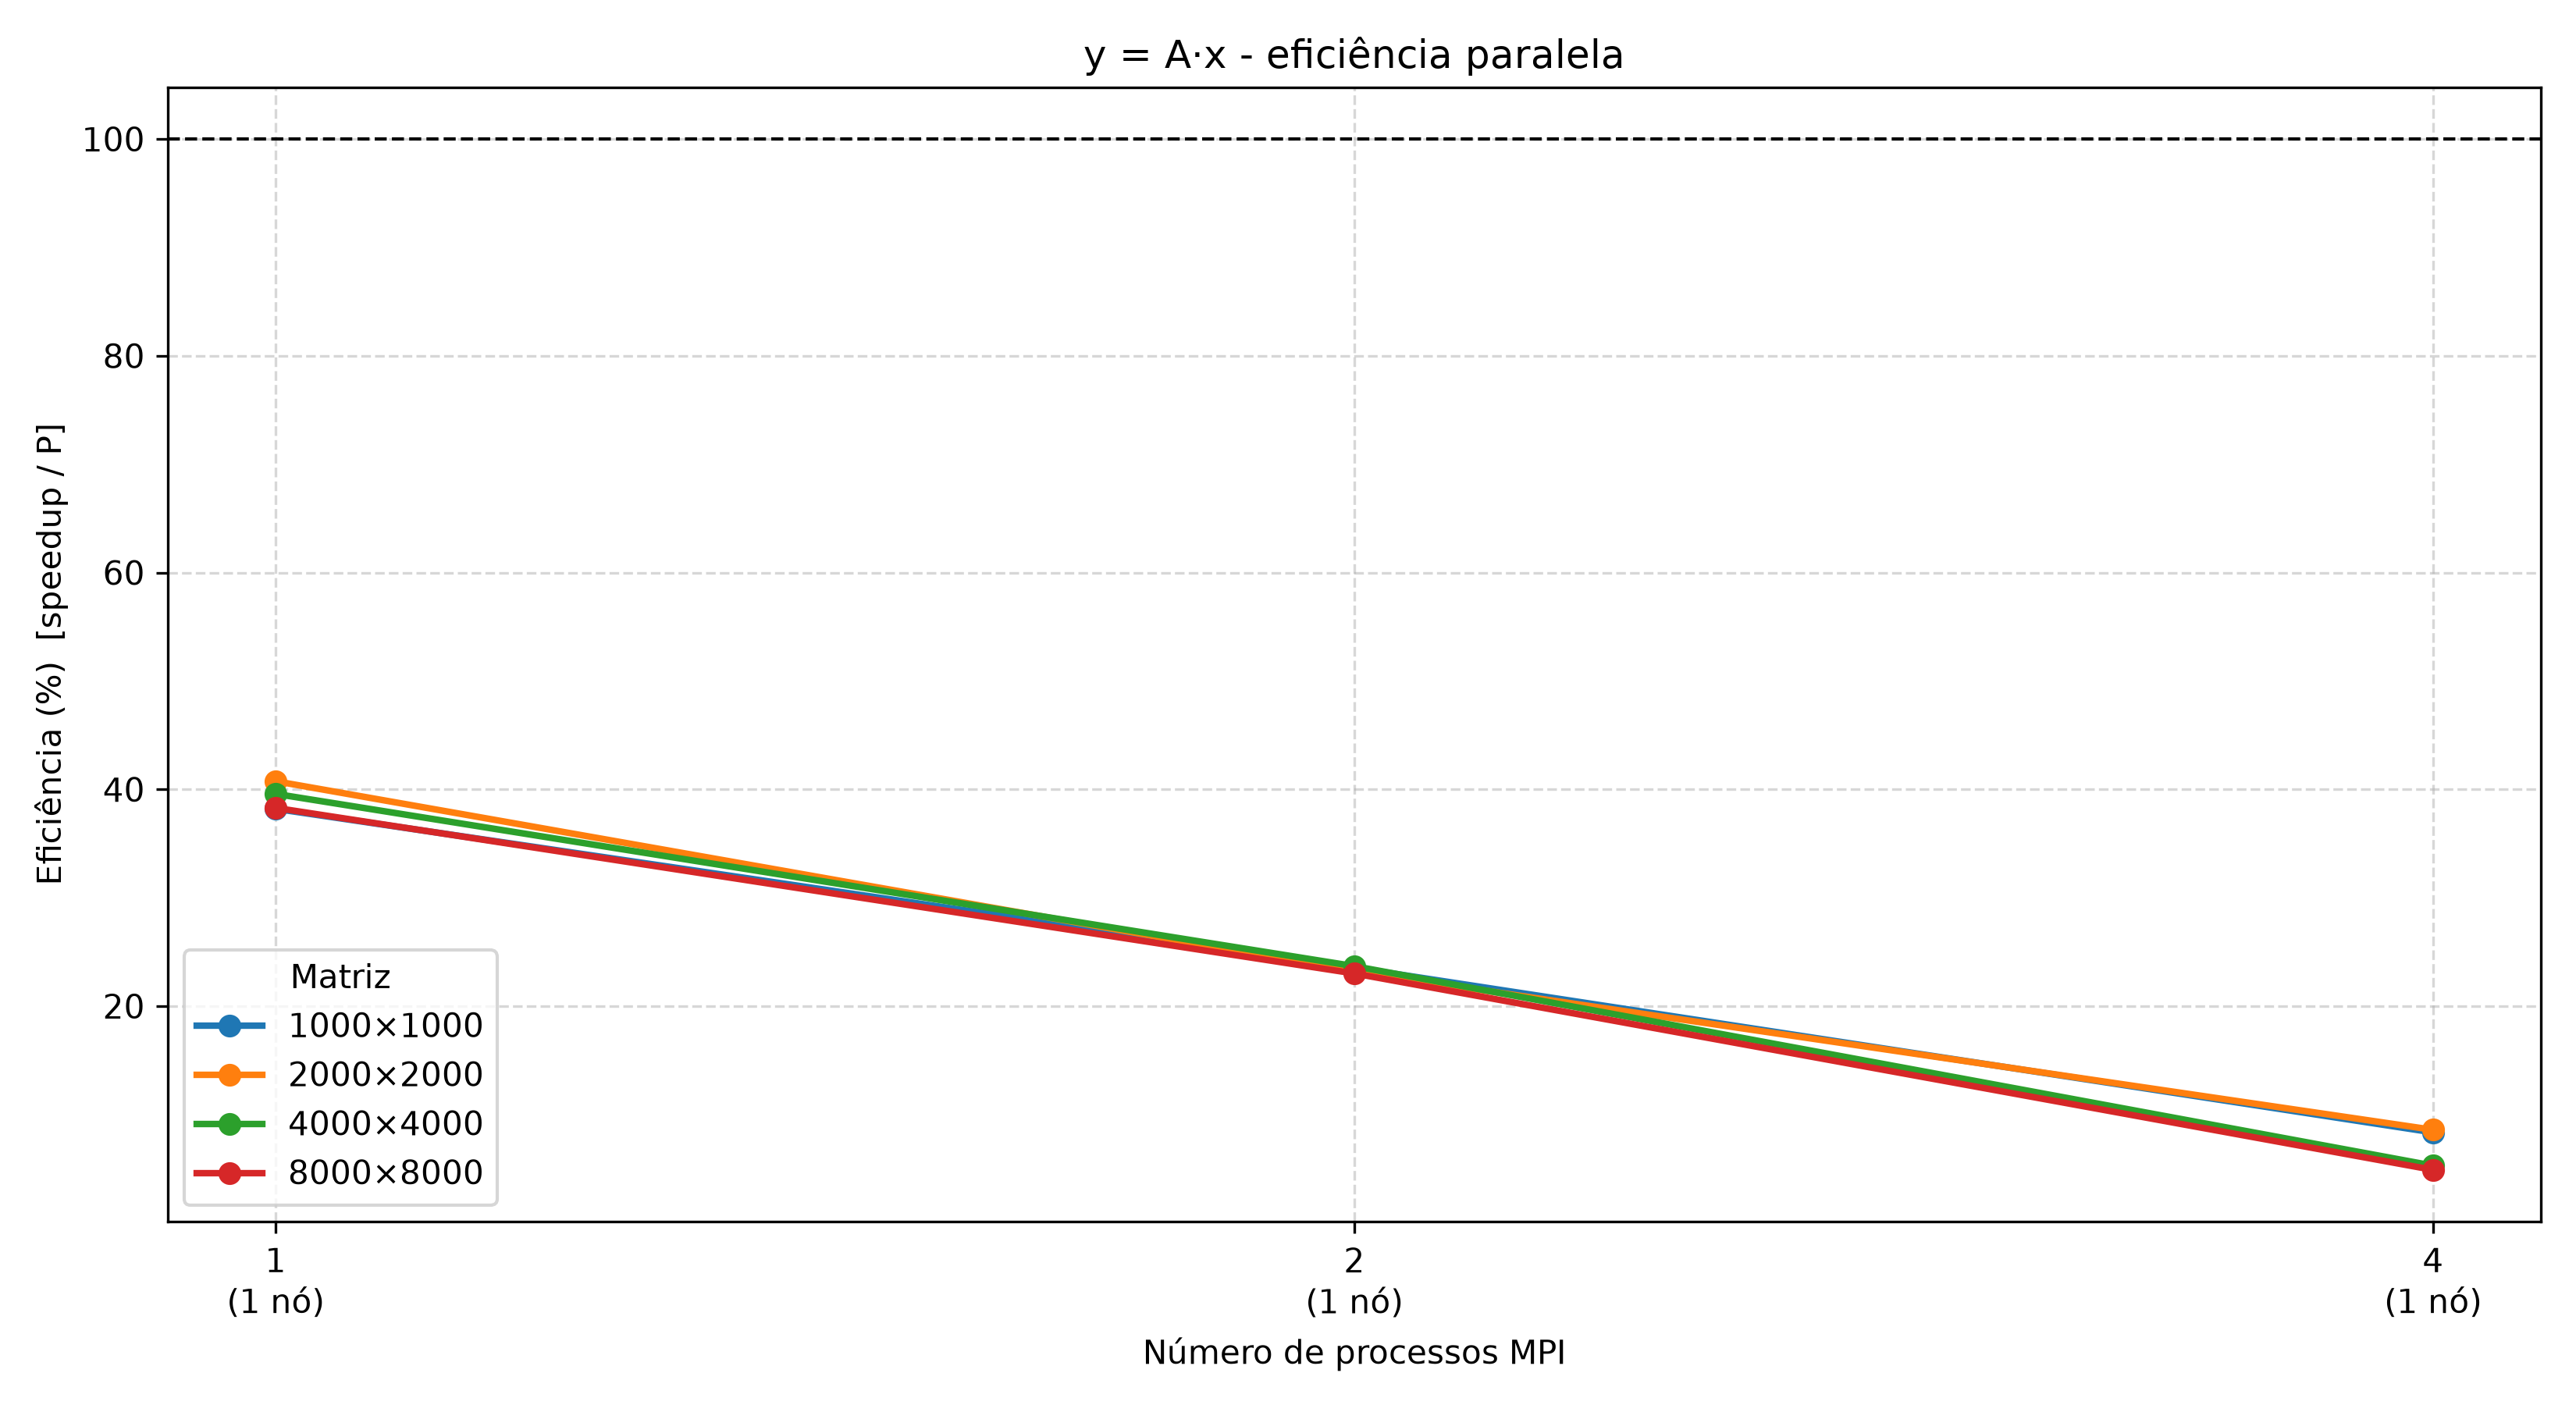
\includegraphics[width=\linewidth]{Tarefa19/tarefa19_eficiencia.png}
	\end{figure}
	\begin{figure}[H]
		\centering
		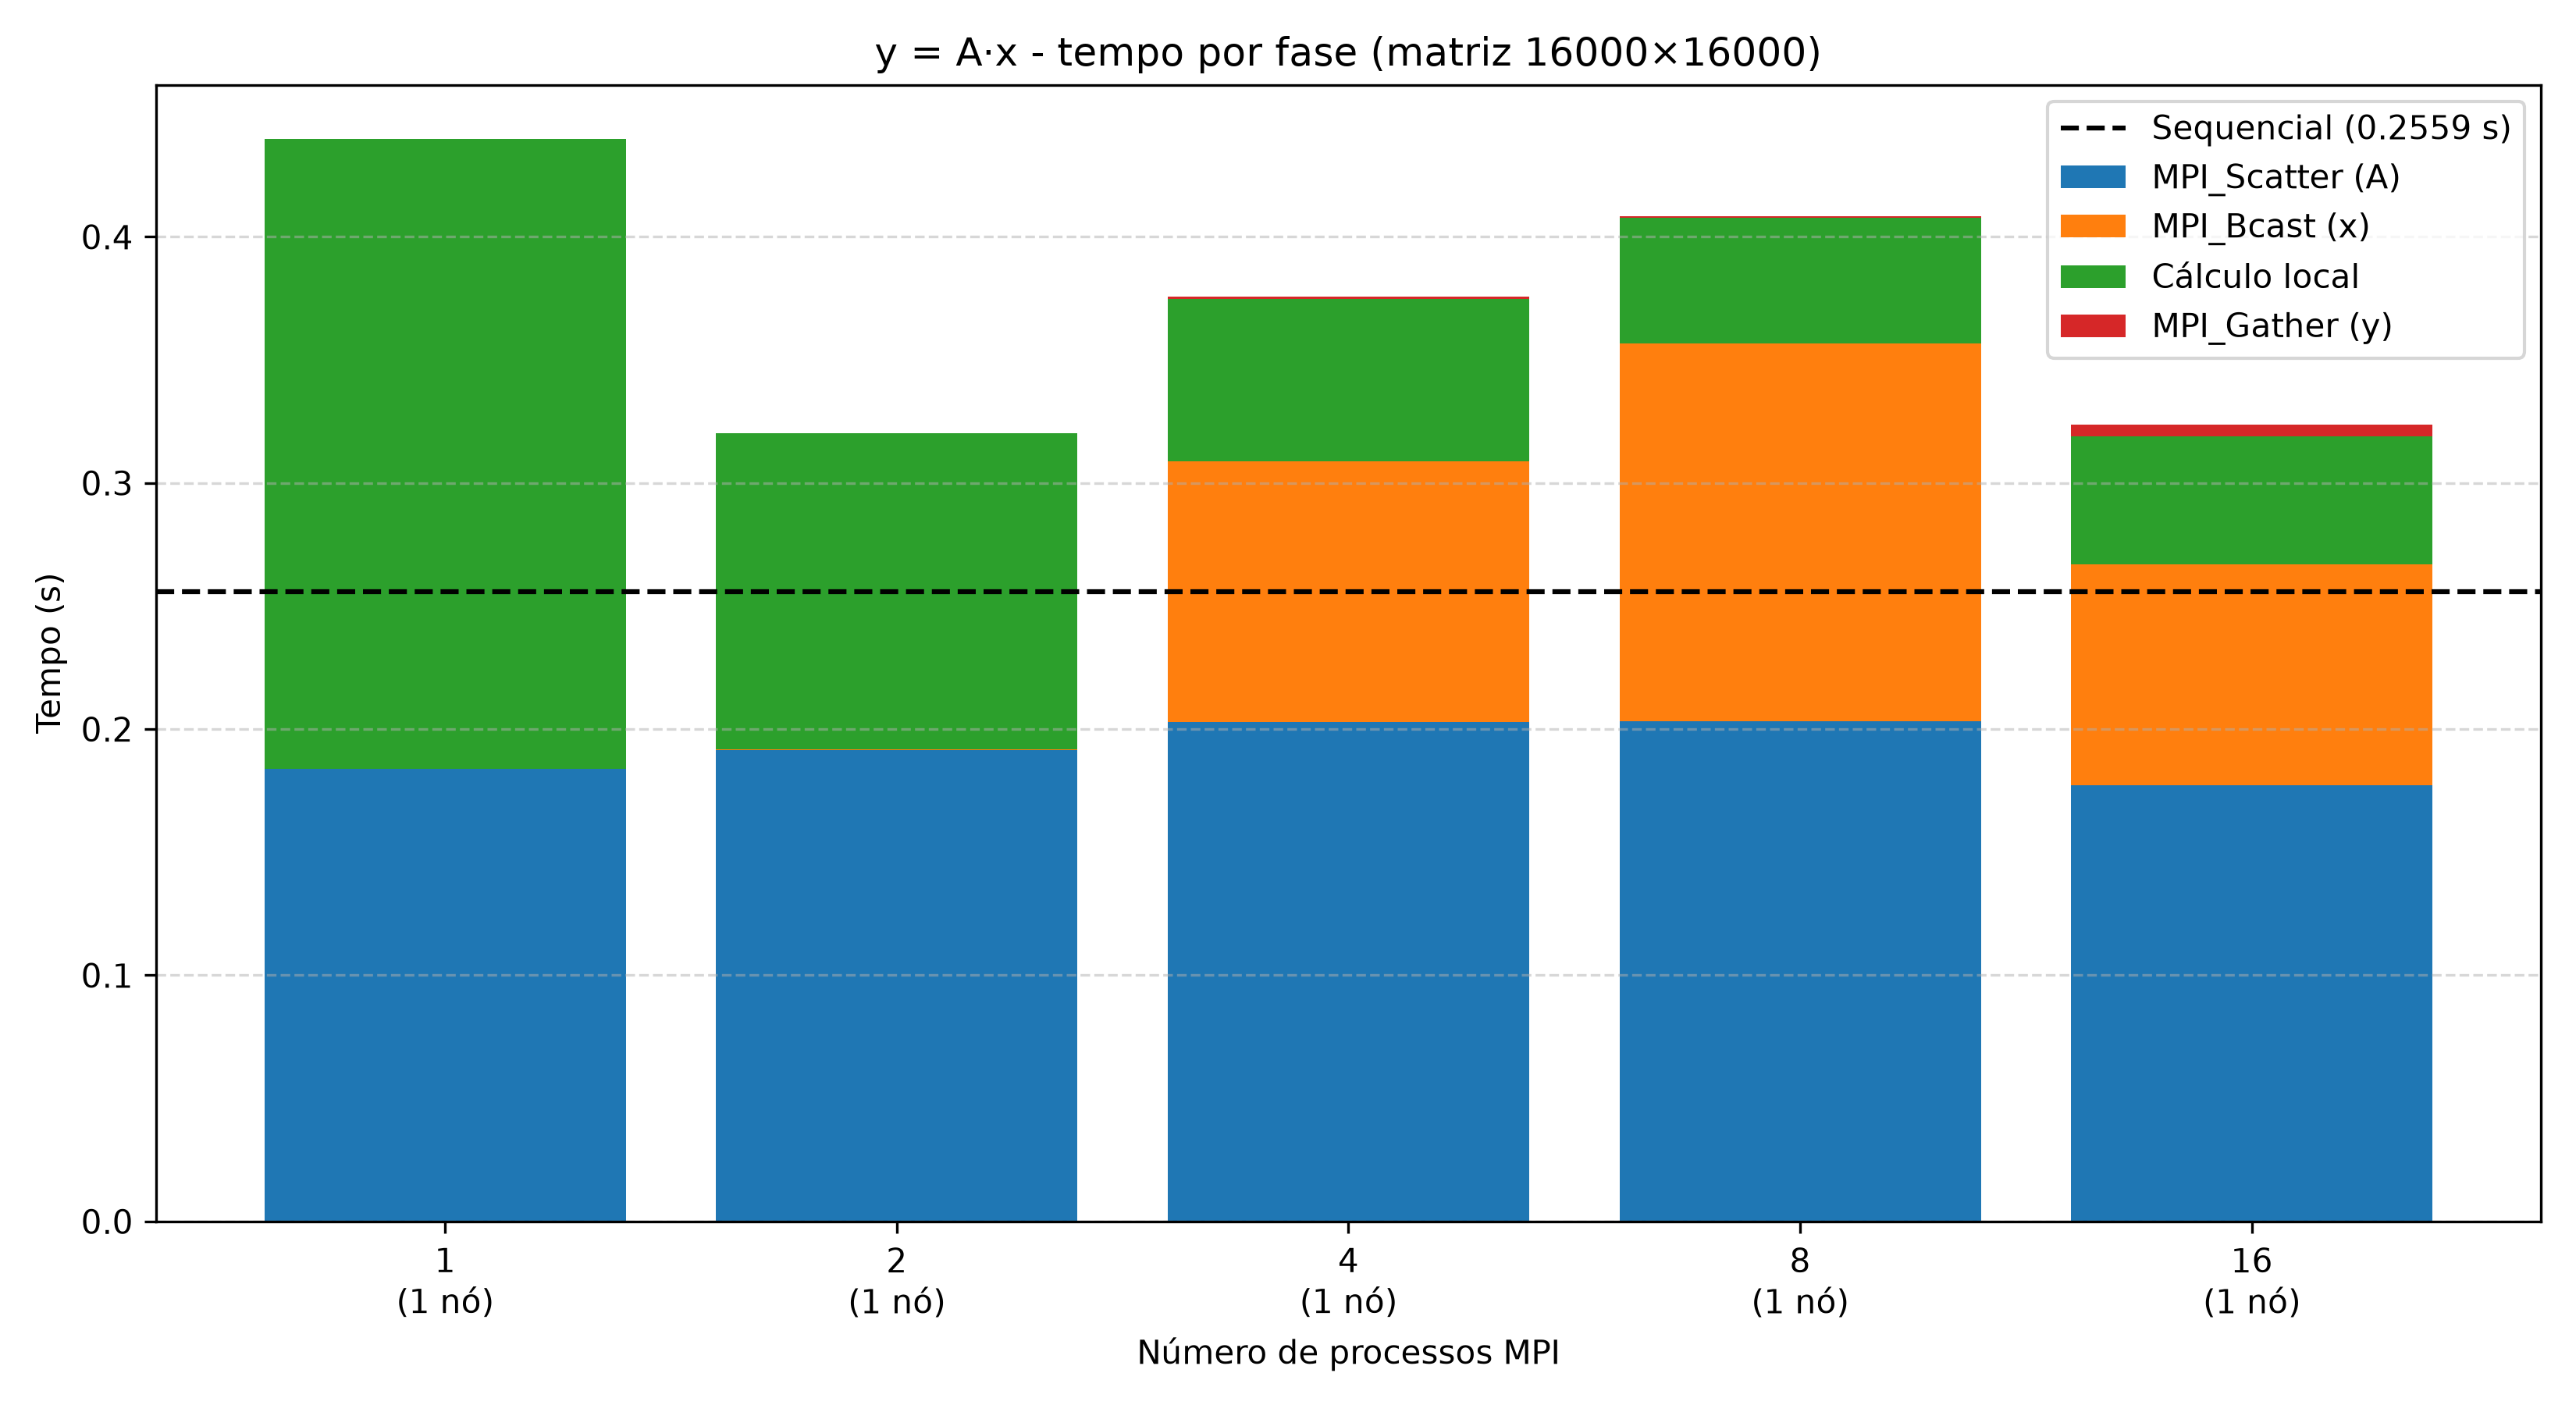
\includegraphics[width=\linewidth]{Tarefa19/tarefa19_fases.png}
	\end{figure}
	\par{
		Os testes foram feitos com matrizes de 1000 a 16000 linhas e de 1 a 16 processos em um único nó, pois a execução em dois nós falhou por um erro na rede do NPAD.
		
		Analisando as fases, a distribuição da matriz com MPI\_Scatter domina o tempo total, já que o processo 0 precisa enviar a matriz inteira. Por isso, o speedup total ficou próximo de 1 e a eficiência caiu para cerca de 7\% com 16 processos. Considerando apenas o cálculo, o speedup chegou a cerca de 5, limitado pela banda da memória do nó.
		
		Portanto, essa paralelização só compensa quando a matriz já está distribuída entre os processos ou é reutilizada em vários cálculos.
	}
	\subsection{\subtTres}
	\begin{lstlisting}[language=c, title=main.c]
#include <math.h>
#include <mpi.h>
#include <stdio.h>
#include <stdlib.h>
#include <string.h>

#define RAIZ 0
#define REPETICOES 5

static const size_t tamanhos[] = {1000, 2000, 4000, 8000, 12000, 16000};
static const size_t quantidade_tamanhos =
    sizeof(tamanhos) / sizeof(tamanhos[0]);

static inline double valor_a(size_t i, size_t j)
{
    return (double)((i * 7 + j * 3) % 17) * 0.125;
}

static inline double valor_x(size_t j) { return 1.0 / (double)(j % 100 + 1); }

static void matvec(const double *A, const double *x, double *y, size_t linhas,
                   size_t n)
{
    for (size_t i = 0; i < linhas; i++) {
        const double *linha = A + i * n;
        double soma = 0.0;
        for (size_t j = 0; j < n; j++) soma += linha[j] * x[j];
        y[i] = soma;
    }
}

int main(int argc, char *argv[])
{
    MPI_Init(&argc, &argv);

    int rank, processos;
    MPI_Comm_rank(MPI_COMM_WORLD, &rank);
    MPI_Comm_size(MPI_COMM_WORLD, &processos);

    size_t limite = argc > 1 ? (size_t)atol(argv[1]) : (size_t)-1;

    char no[MPI_MAX_PROCESSOR_NAME];
    int tam_nome;
    memset(no, 0, sizeof(no));
    MPI_Get_processor_name(no, &tam_nome);
    char *nomes = NULL;
    if (rank == RAIZ) nomes = malloc((size_t)processos * MPI_MAX_PROCESSOR_NAME);
    MPI_Gather(no, MPI_MAX_PROCESSOR_NAME, MPI_CHAR, nomes,
               MPI_MAX_PROCESSOR_NAME, MPI_CHAR, RAIZ, MPI_COMM_WORLD);

    FILE *json = NULL;
    if (rank == RAIZ) {
        int nos = 0;
        for (int p = 0; p < processos; p++) {
            int novo = 1;
            for (int q = 0; q < p; q++)
                if (strcmp(nomes + p * MPI_MAX_PROCESSOR_NAME,
                           nomes + q * MPI_MAX_PROCESSOR_NAME) == 0) {
                    novo = 0;
                    break;
                }
            nos += novo;
        }

        char nome_arquivo[64];
        snprintf(nome_arquivo, sizeof(nome_arquivo), "resultados_np%d.json",
                 processos);
        json = fopen(nome_arquivo, "w");
        if (json == NULL) {
            fprintf(stderr, "Erro ao abrir %s\n", nome_arquivo);
            MPI_Abort(MPI_COMM_WORLD, 1);
        }
        fprintf(json, "{\n  \"processos\": %d,\n  \"nos\": %d,\n", processos,
                nos);
        fprintf(json, "  \"repeticoes\": %d,\n  \"resultados\": [\n",
                REPETICOES);

        printf("y = A.x com %d processos em %d no(s)\n", processos, nos);
        printf("%7s | %10s %10s %10s %10s %10s | %10s %8s %8s | %s\n", "N",
               "scatter", "bcast", "calculo", "gather", "total", "seq",
               "speedup", "efic.", "erro");
    }

    int primeiro = 1;

    for (size_t t = 0; t < quantidade_tamanhos; t++) {
        size_t m = tamanhos[t];
        size_t n = tamanhos[t];
        if (m > limite) break;

        size_t linhas_local = (m + processos - 1) / processos;
        size_t m_pad = linhas_local * processos;

        double *A = NULL, *y = NULL, *y_seq = NULL;
        double *x = malloc(n * sizeof(double));
        double *A_local = malloc(linhas_local * n * sizeof(double));
        double *y_local = malloc(linhas_local * sizeof(double));

        if (rank == RAIZ) {
            A = calloc(m_pad * n, sizeof(double));
            y = malloc(m_pad * sizeof(double));
            y_seq = malloc(m * sizeof(double));
            if (!A || !y || !y_seq) {
                fprintf(stderr, "Erro de alocacao (N = %zu)\n", n);
                MPI_Abort(MPI_COMM_WORLD, 1);
            }
            for (size_t i = 0; i < m; i++)
                for (size_t j = 0; j < n; j++) A[i * n + j] = valor_a(i, j);
            for (size_t j = 0; j < n; j++) x[j] = valor_x(j);
        }
        if (!x || !A_local || !y_local) {
            fprintf(stderr, "Erro de alocacao (N = %zu)\n", n);
            MPI_Abort(MPI_COMM_WORLD, 1);
        }

        double tempo_seq = 0.0;
        if (rank == RAIZ) {
            for (int r = 0; r < REPETICOES; r++) {
                double t0 = MPI_Wtime();
                matvec(A, x, y_seq, m, n);
                tempo_seq += MPI_Wtime() - t0;
            }
            tempo_seq /= REPETICOES;
        }

        int contagem = (int)(linhas_local * n);
        double soma_fases[5] = {0, 0, 0, 0, 0};

        for (int r = 0; r < REPETICOES; r++) {
            MPI_Barrier(MPI_COMM_WORLD);
            double t0 = MPI_Wtime();

            MPI_Scatter(A, contagem, MPI_DOUBLE, A_local, contagem,
                        MPI_DOUBLE, RAIZ, MPI_COMM_WORLD);
            double t1 = MPI_Wtime();

            MPI_Bcast(x, (int)n, MPI_DOUBLE, RAIZ, MPI_COMM_WORLD);
            double t2 = MPI_Wtime();

            matvec(A_local, x, y_local, linhas_local, n);
            double t3 = MPI_Wtime();

            MPI_Gather(y_local, (int)linhas_local, MPI_DOUBLE, y,
                       (int)linhas_local, MPI_DOUBLE, RAIZ, MPI_COMM_WORLD);
            double t4 = MPI_Wtime();

            double locais[5] = {t1 - t0, t2 - t1, t3 - t2, t4 - t3, t4 - t0};
            double maximos[5];
            MPI_Reduce(locais, maximos, 5, MPI_DOUBLE, MPI_MAX, RAIZ,
                       MPI_COMM_WORLD);
            if (rank == RAIZ)
                for (int f = 0; f < 5; f++) soma_fases[f] += maximos[f];
        }

        if (rank == RAIZ) {
            double fases[5];
            for (int f = 0; f < 5; f++) fases[f] = soma_fases[f] / REPETICOES;

            double erro = 0.0;
            for (size_t i = 0; i < m; i++) {
                double d = fabs(y[i] - y_seq[i]);
                if (d > erro) erro = d;
            }

            double speedup = tempo_seq / fases[4];
            double eficiencia = speedup / processos;
            double speedup_calculo = tempo_seq / fases[2];

            printf("%7zu | %10.5f %10.5f %10.5f %10.5f %10.5f | %10.5f %8.2f "
                   "%7.1f%% | %.1e\n",
                   n, fases[0], fases[1], fases[2], fases[3], fases[4],
                   tempo_seq, speedup, 100 * eficiencia, erro);

            fprintf(json,
                    "%s    {\"m\": %zu, \"n\": %zu, \"linhas_por_processo\": "
                    "%zu, \"tempo_scatter_s\": %.9f, \"tempo_bcast_s\": %.9f, "
                    "\"tempo_calculo_s\": %.9f, \"tempo_gather_s\": %.9f, "
                    "\"tempo_total_s\": %.9f, \"tempo_sequencial_s\": %.9f, "
                    "\"speedup\": %f, \"eficiencia\": %f, "
                    "\"speedup_calculo\": %f, \"erro_max\": %g}",
                    primeiro ? "" : ",\n", m, n, linhas_local, fases[0],
                    fases[1], fases[2], fases[3], fases[4], tempo_seq,
                    speedup, eficiencia, speedup_calculo, erro);
            primeiro = 0;
        }

        free(A);
        free(y);
        free(y_seq);
        free(x);
        free(A_local);
        free(y_local);
    }

    if (rank == RAIZ) {
        fprintf(json, "\n  ]\n}\n");
        fclose(json);
        free(nomes);
        printf("Resultados salvos em resultados_np%d.json\n", processos);
    }

    MPI_Finalize();
    return 0;
}
\end{lstlisting}
	\begin{lstlisting}[language=bash, title=script\_mpi.sh]
#!/bin/bash
#SBATCH --job-name=MPI_matvec_akira
#SBATCH --output=saida%j.out
#SBATCH --error=erro%j.err
#SBATCH --partition=amd-512
#SBATCH --nodes=2
#SBATCH --ntasks-per-node=16
#SBATCH --time=0-0:30

cd "${SLURM_SUBMIT_DIR:-.}"
mkdir -p outputs

MPIRUN_OPTS=""
if mpirun --version 2>&1 | grep -qi "open mpi"; then
    MPIRUN_OPTS="--mca btl ^openib"
fi

echo "===== Build ====="
mpicc -O2 main.c -o outputs/main -lm || exit 1

for np in 1 2 4 8 16 32; do
    echo "===== ${np} processos ====="
    mpirun -np ${np} ${MPIRUN_OPTS} ./outputs/main
done

echo "===== Graficos ====="
if command -v python3 > /dev/null 2>&1 && python3 -c "import matplotlib" 2> /dev/null; then
    python3 plot.py
else
    echo "matplotlib indisponivel: copie os resultados_np*.json e rode plot.py localmente."
fi
\end{lstlisting}
	
	\newpage
	\onehalfspacing
	\section{TAREFA 20}
	\subsection{\subtUm}
	\par{Desenvolver um programa paralelo para calcular a integral definida de uma função utilizando o método do trapézio.
		
		O programa deve dividir o trabalho entre os processos MPI com paralelismo local, tolerância a falhas, redução global e validação do resultado.
		
		Analisar os resultados, comparando o desempenho da execução utilizando CPU e GPU, avaliando o impacto da comunicação entre os nós no tempo total de execução.}
	\subsection{\subtDois}
	\begin{figure}[H]
		\centering
		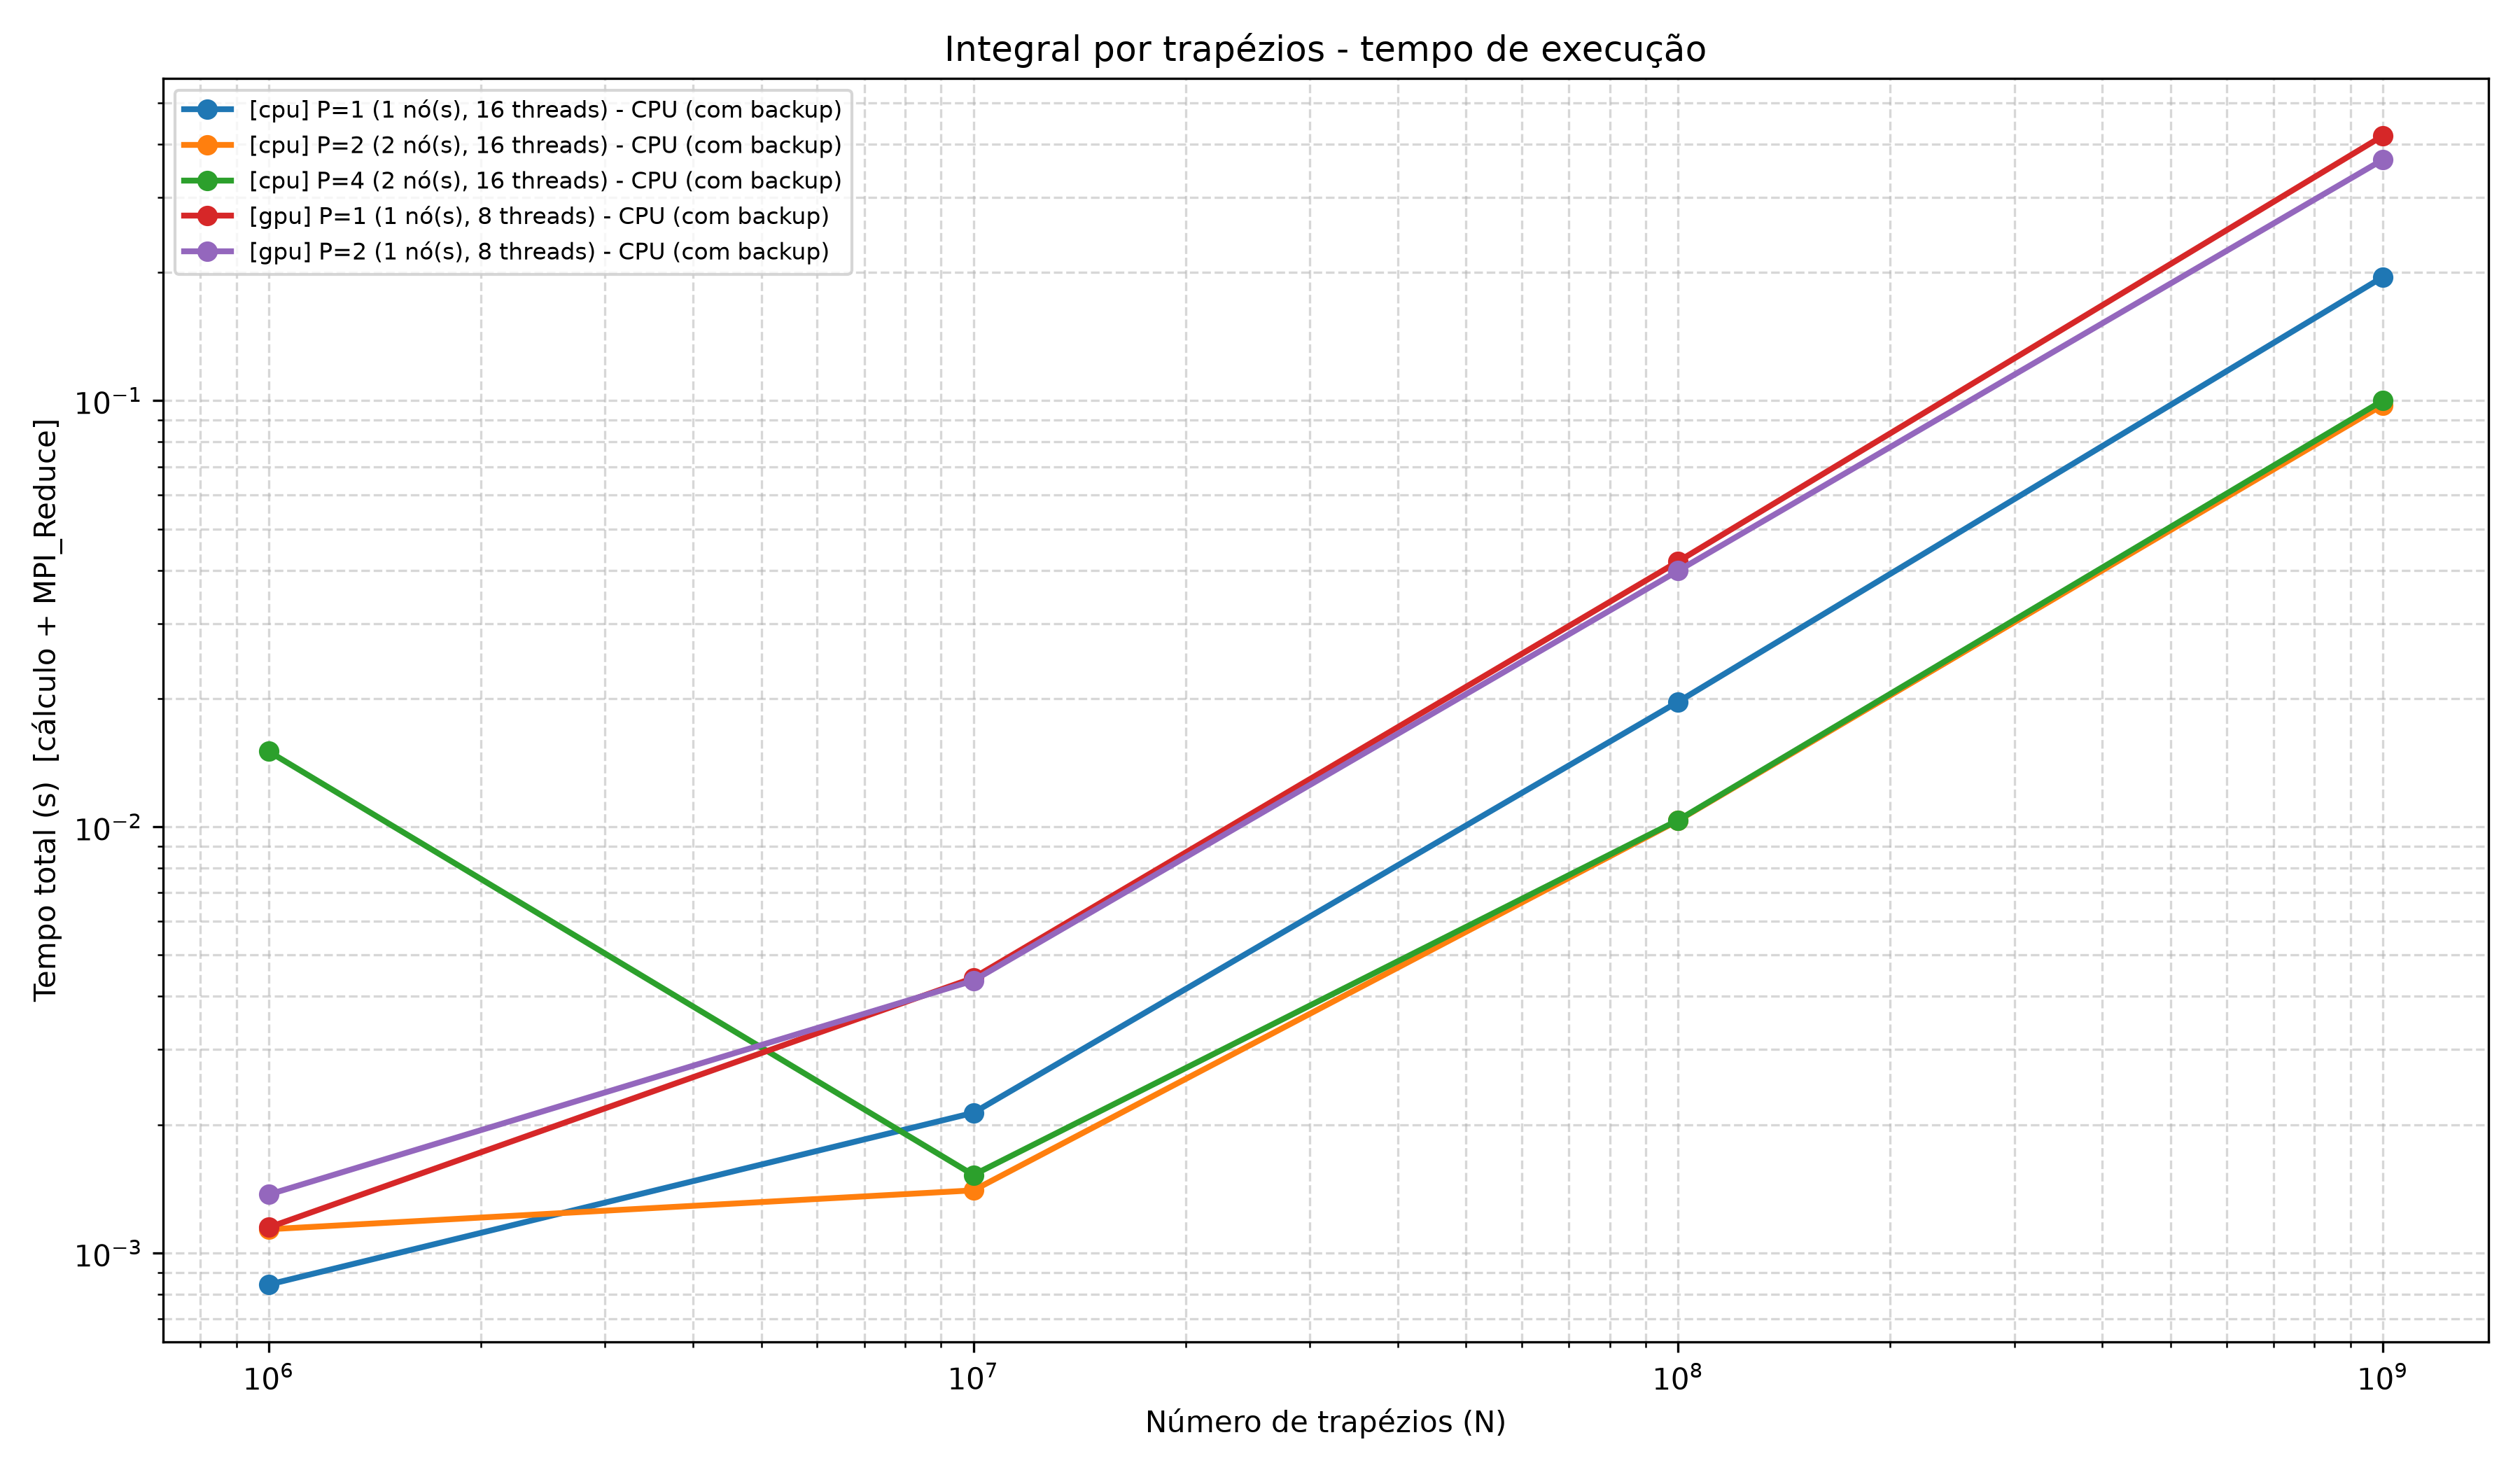
\includegraphics[width=\linewidth]{Tarefa20/tarefa20_tempo.png}
	\end{figure}
	\begin{figure}[H]
		\centering
		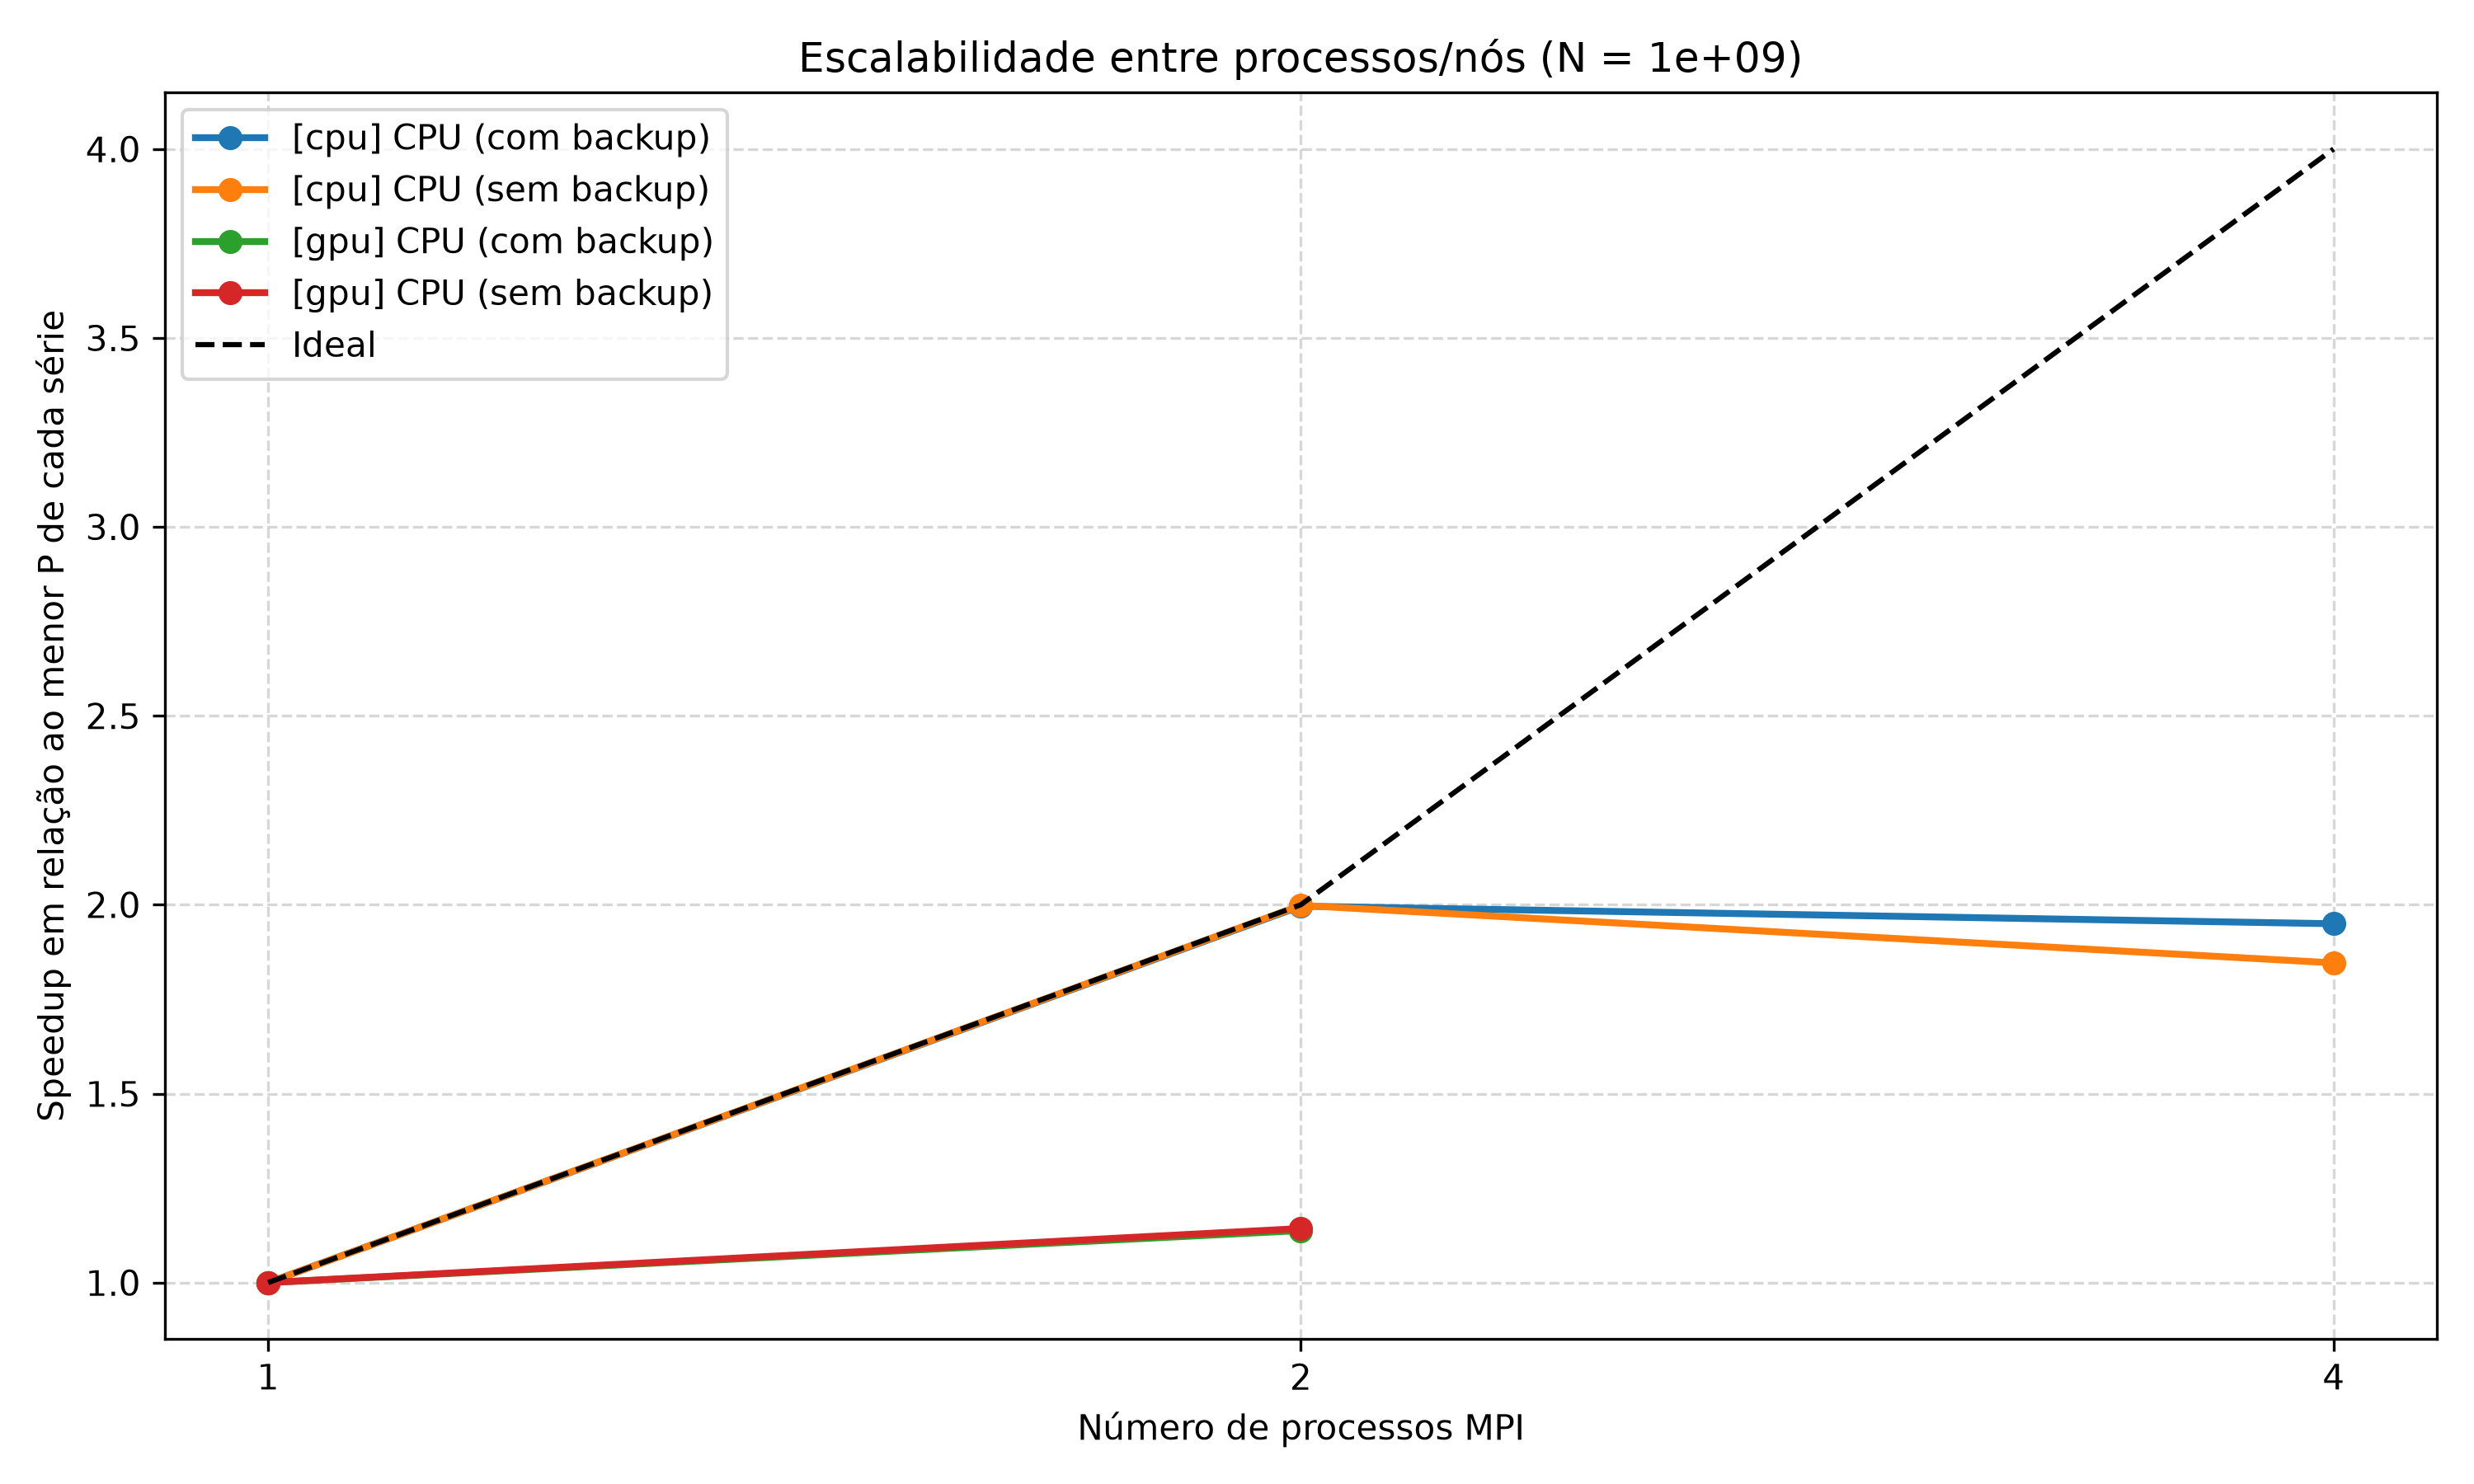
\includegraphics[width=\linewidth]{Tarefa20/tarefa20_escala.png}
	\end{figure}
	\begin{figure}[H]
		\centering
		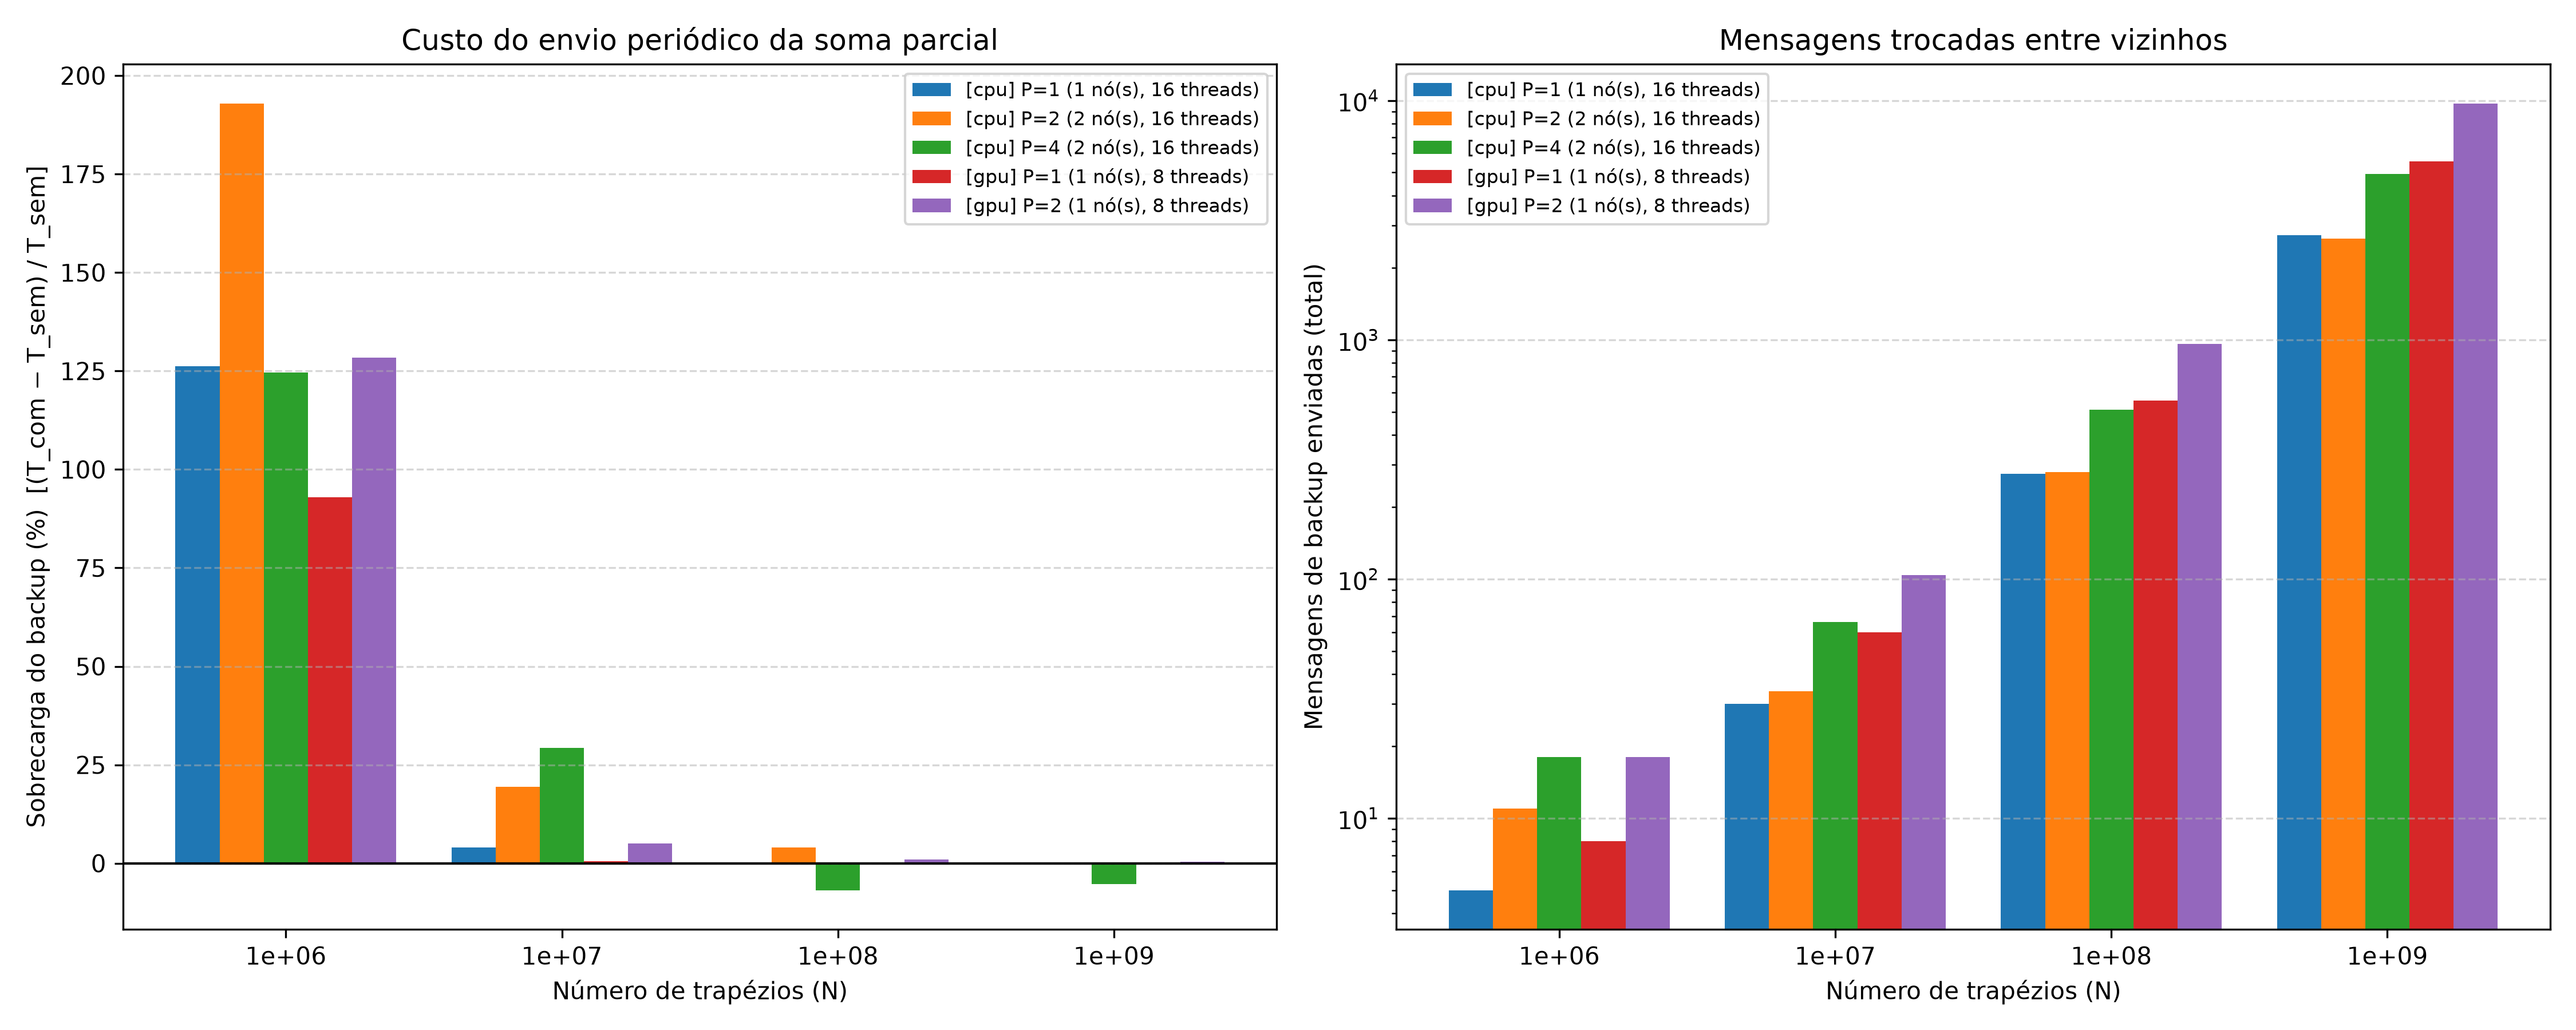
\includegraphics[width=\linewidth]{Tarefa20/tarefa20_comunicacao.png}
	\end{figure}
	\begin{figure}[H]
		\centering
		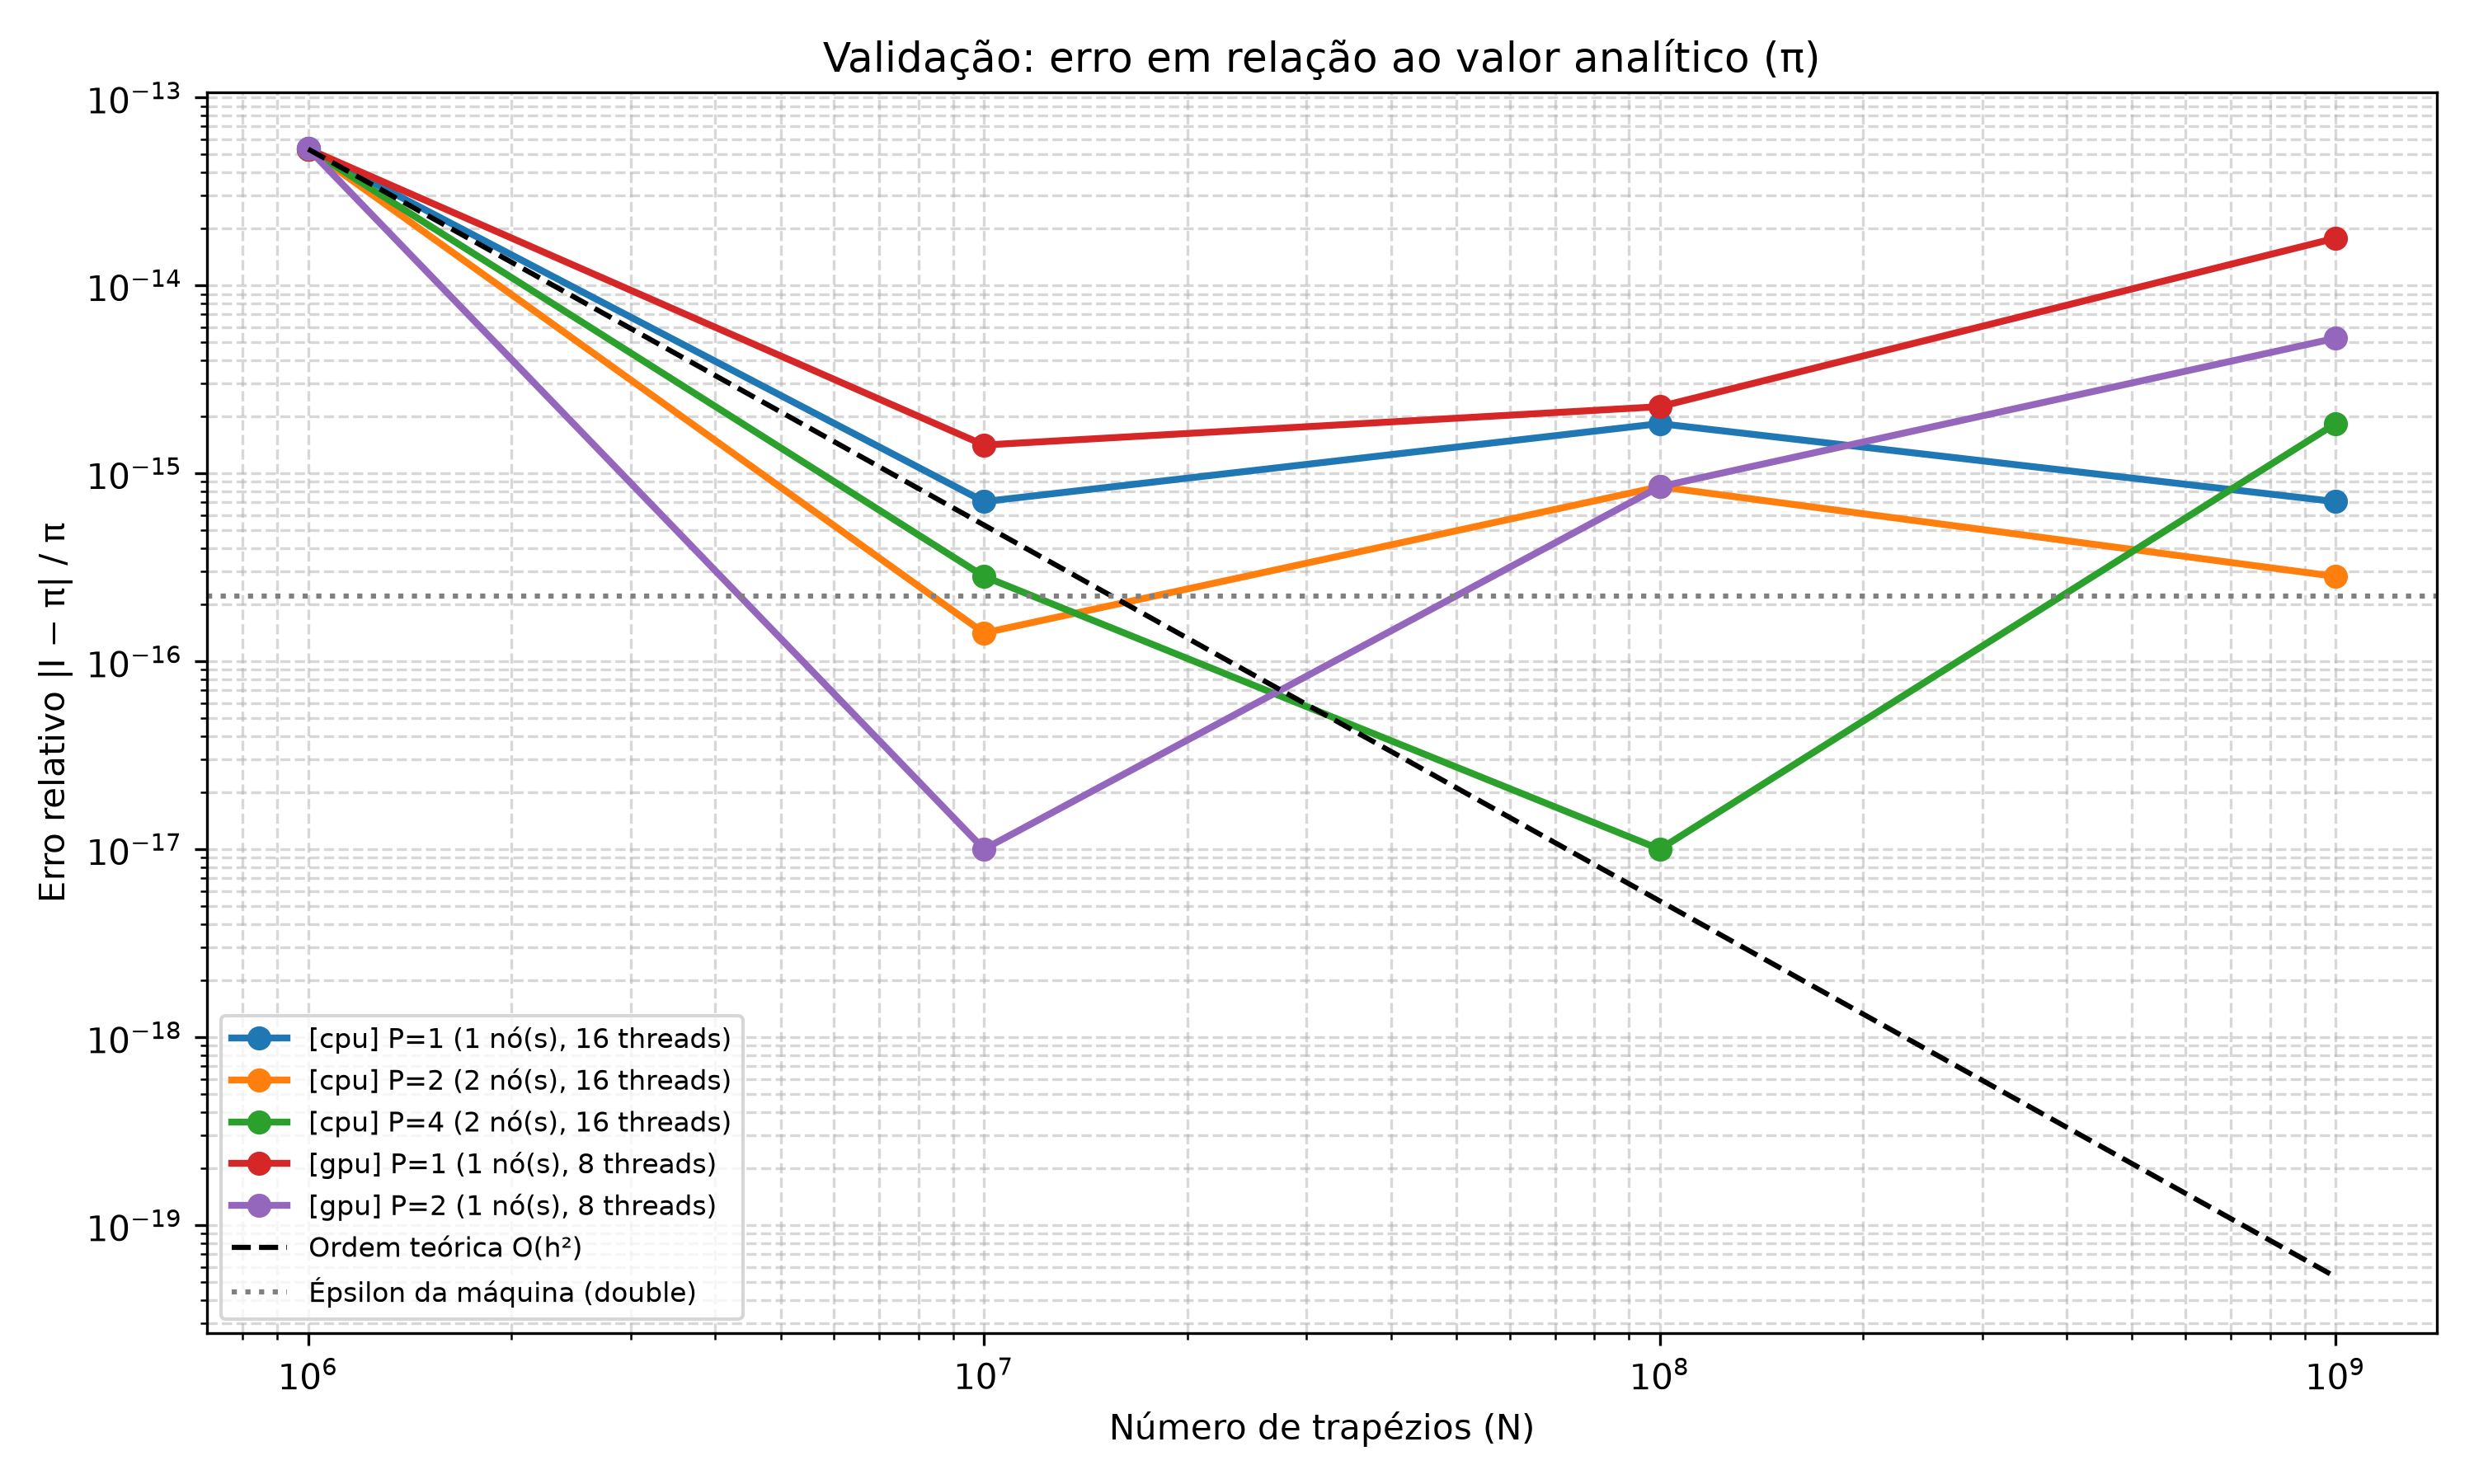
\includegraphics[width=\linewidth]{Tarefa20/tarefa20_erro.png}
	\end{figure}
	\par{
		O resultado foi validado com o valor exato de pi, com erro relativo entre $10^{-16}$ e $10^{-13}$, e o backup guardado por cada processo foi igual à soma final do vizinho em todas as execuções.
		
		Na CPU, com 16 threads por processo, o cálculo com 1 bilhão de trapézios levou 0,195 s com um processo e 0,098 s com dois processos em dois nós, um speedup de 2. A comunicação entre os nós teve impacto desprezível, pois a redução final e o envio do backup ao vizinho levam microssegundos, perto do tempo de cálculo.
		
		A execução com GPU foi feita em apenas um nó, com dois processos e uma GPU para cada um, pois as partições com GPU do NPAD não tinham dois nós disponíveis no momento dos testes. Nessa execução, o código para a placa de vídeo não foi gerado, pois o compilador da NVIDIA não aceitou uma das diretivas do OpenMP usadas no programa, e o cálculo foi feito na CPU, com 8 threads por processo, levando 0,42 s com um processo e 0,37 s com dois. Portanto, para este problema, que exige muito cálculo e pouca comunicação, a divisão do trabalho entre processos e threads escala bem.
	}
	\subsection{\subtTres}
	\begin{lstlisting}[language=c, title=main.c]
#include <math.h>
#include <mpi.h>
#include <omp.h>
#include <stdio.h>
#include <stdlib.h>
#include <string.h>
#include <time.h>

#define RAIZ 0
#define AMOSTRAS_CHECKPOINT 100
#define BLOCOS_POR_PEGADA 1000
#define LOTES_GPU 64
#define TAG_BACKUP 77
#define PAUSA_COMUNICACAO_NS 20000

#define A_INTERVALO 0.0
#define B_INTERVALO 1.0
#define VALOR_EXATO 3.14159265358979323846

static const size_t quantidades[] = {1000000, 10000000, 100000000,
                                     1000000000};
static const size_t total_quantidades =
    sizeof(quantidades) / sizeof(quantidades[0]);

#pragma omp declare target
static inline double f(double x) { return 4.0 / (1.0 + x * x); }
#pragma omp end declare target

typedef struct {
    double soma;
    long long amostras;
    char preenchimento[64 - sizeof(double) - sizeof(long long)];
} Progresso;

typedef struct {
    double soma;
    double amostras;
    double final;
} Backup;

typedef enum { MODO_CPU, MODO_CPU_SEM_BACKUP, MODO_GPU } Modo;

static const char *nome_modo(Modo m)
{
    switch (m) {
    case MODO_CPU: return "cpu";
    case MODO_CPU_SEM_BACKUP: return "cpu_sem_backup";
    case MODO_GPU: return "gpu";
    }
    return "?";
}

static int gpu_disponivel(void)
{
    if (omp_get_num_devices() <= 0) return 0;
    int no_host = 1;
#pragma omp target map(from : no_host)
    {
        no_host = omp_is_initial_device();
    }
    return !no_host;
}

static double soma_trapezios(size_t ini, size_t fim, double h)
{
    double s = 0.0;
    for (size_t i = ini; i < fim; i++) {
        double x0 = A_INTERVALO + i * h;
        s += 0.5 * h * (f(x0) + f(x0 + h));
    }
    return s;
}

static double soma_trapezios_gpu(size_t ini, size_t fim, double h)
{
    double s = 0.0;
#pragma omp target teams distribute parallel for reduction(+ : s) \
    map(tofrom : s)
    for (size_t i = ini; i < fim; i++) {
        double x0 = A_INTERVALO + i * h;
        s += 0.5 * h * (f(x0) + f(x0 + h));
    }
    return s;
}

typedef struct {
    double soma_local;
    double tempo_calculo;
    long long mensagens_enviadas;
    long long mensagens_recebidas;
    double backup_soma;
    double backup_amostras;
} ResultadoLocal;

static ResultadoLocal calcula_parcela(size_t ini, size_t fim, double h,
                                      Modo modo, int rank, int processos,
                                      int threads)
{
    ResultadoLocal res;
    memset(&res, 0, sizeof(res));

    size_t total_local = fim - ini;
    size_t total_blocos =
        (total_local + AMOSTRAS_CHECKPOINT - 1) / AMOSTRAS_CHECKPOINT;

    Progresso *progresso = calloc(threads, sizeof(Progresso));
    size_t proxima_pegada = 0;
    int calculadoras_ativas = threads - 1;

    int direita = (rank + 1) % processos;
    int esquerda = (rank - 1 + processos) % processos;

    double t0 = MPI_Wtime();

#pragma omp parallel num_threads(threads)
    {
        int tid = omp_get_thread_num();

        if (tid != 0) {

            double minha_soma = 0.0;
            long long minhas_amostras = 0;

            if (modo == MODO_GPU) {

                if (tid == 1) {
                    size_t tam_lote = (total_local + LOTES_GPU - 1) / LOTES_GPU;
                    tam_lote = ((tam_lote + AMOSTRAS_CHECKPOINT - 1) /
                                AMOSTRAS_CHECKPOINT) * AMOSTRAS_CHECKPOINT;
                    if (tam_lote == 0) tam_lote = AMOSTRAS_CHECKPOINT;

                    for (size_t a = ini; a < fim; a += tam_lote) {
                        size_t b = a + tam_lote < fim ? a + tam_lote : fim;
                        minha_soma += soma_trapezios_gpu(a, b, h);
                        minhas_amostras += (long long)(b - a);
#pragma omp atomic write
                        progresso[tid].soma = minha_soma;
#pragma omp atomic write
                        progresso[tid].amostras = minhas_amostras;
                    }
                }
            } else {

                while (1) {
                    size_t pegada;
#pragma omp atomic capture
                    pegada = proxima_pegada++;

                    size_t bloco_ini = pegada * BLOCOS_POR_PEGADA;
                    if (bloco_ini >= total_blocos) break;
                    size_t bloco_fim = bloco_ini + BLOCOS_POR_PEGADA;
                    if (bloco_fim > total_blocos) bloco_fim = total_blocos;

                    for (size_t bl = bloco_ini; bl < bloco_fim; bl++) {
                        size_t a = ini + bl * AMOSTRAS_CHECKPOINT;
                        size_t b = a + AMOSTRAS_CHECKPOINT;
                        if (b > fim) b = fim;

                        minha_soma += soma_trapezios(a, b, h);
                        minhas_amostras += (long long)(b - a);
#pragma omp atomic write
                        progresso[tid].soma = minha_soma;
#pragma omp atomic write
                        progresso[tid].amostras = minhas_amostras;
                    }
                }
            }

#pragma omp flush
#pragma omp atomic update
            calculadoras_ativas--;
        } else {

            Backup envio, recebido;
            MPI_Request req_envio = MPI_REQUEST_NULL;
            long long ultimo_enviado = 0;
            int recebeu_final = (modo == MODO_CPU_SEM_BACKUP);
            int enviou_final = (modo == MODO_CPU_SEM_BACKUP);

            while (!enviou_final || !recebeu_final) {
                int ativas;
#pragma omp atomic read
                ativas = calculadoras_ativas;
#pragma omp flush

                double soma = 0.0;
                long long amostras = 0;
                for (int t = 1; t < threads; t++) {
                    double s;
                    long long a;
#pragma omp atomic read
                    s = progresso[t].soma;
#pragma omp atomic read
                    a = progresso[t].amostras;
                    soma += s;
                    amostras += a;
                }

                if (modo != MODO_CPU_SEM_BACKUP) {

                    int livre = 1;
                    if (req_envio != MPI_REQUEST_NULL)
                        MPI_Test(&req_envio, &livre, MPI_STATUS_IGNORE);

                    if (livre && !enviou_final) {
                        int terminou = ativas == 0;
                        if (terminou ||
                            amostras - ultimo_enviado >= AMOSTRAS_CHECKPOINT) {
                            if (terminou) {

                                soma = 0.0;
                                amostras = 0;
                                for (int t = 1; t < threads; t++) {
                                    double s;
                                    long long a;
#pragma omp atomic read
                                    s = progresso[t].soma;
#pragma omp atomic read
                                    a = progresso[t].amostras;
                                    soma += s;
                                    amostras += a;
                                }
                            }
                            envio.soma = soma;
                            envio.amostras = (double)amostras;
                            envio.final = terminou ? 1.0 : 0.0;
                            MPI_Isend(&envio, 3, MPI_DOUBLE, direita,
                                      TAG_BACKUP, MPI_COMM_WORLD, &req_envio);
                            ultimo_enviado = amostras;
                            res.mensagens_enviadas++;
                            if (terminou) enviou_final = 1;
                        }
                    }

                    int chegou = 1;
                    while (chegou && !recebeu_final) {
                        MPI_Iprobe(esquerda, TAG_BACKUP, MPI_COMM_WORLD,
                                   &chegou, MPI_STATUS_IGNORE);
                        if (chegou) {
                            MPI_Recv(&recebido, 3, MPI_DOUBLE, esquerda,
                                     TAG_BACKUP, MPI_COMM_WORLD,
                                     MPI_STATUS_IGNORE);
                            res.backup_soma = recebido.soma;
                            res.backup_amostras = recebido.amostras;
                            res.mensagens_recebidas++;
                            if (recebido.final == 1.0) recebeu_final = 1;
                        }
                    }
                } else if (ativas == 0) {
                    break;
                }

                if (!enviou_final || !recebeu_final || ativas > 0) {
                    struct timespec pausa = {0, PAUSA_COMUNICACAO_NS};
                    nanosleep(&pausa, NULL);
                }
            }

            if (req_envio != MPI_REQUEST_NULL)
                MPI_Wait(&req_envio, MPI_STATUS_IGNORE);
        }
    }

    res.tempo_calculo = MPI_Wtime() - t0;

    for (int t = 1; t < threads; t++) res.soma_local += progresso[t].soma;

    free(progresso);
    return res;
}

int main(int argc, char *argv[])
{
    int fornecido;
    MPI_Init_thread(&argc, &argv, MPI_THREAD_FUNNELED, &fornecido);

    int rank, processos;
    MPI_Comm_rank(MPI_COMM_WORLD, &rank);
    MPI_Comm_size(MPI_COMM_WORLD, &processos);

    if (fornecido < MPI_THREAD_FUNNELED) {
        if (rank == RAIZ)
            fprintf(stderr, "A biblioteca MPI nao suporta "
                            "MPI_THREAD_FUNNELED.\n");
        MPI_Abort(MPI_COMM_WORLD, 1);
    }

    const char *rotulo = argc > 1 ? argv[1] : "";

    int threads = omp_get_max_threads();
    if (threads < 2) threads = 2;

    MPI_Comm comm_no;
    int rank_no;
    MPI_Comm_split_type(MPI_COMM_WORLD, MPI_COMM_TYPE_SHARED, rank,
                        MPI_INFO_NULL, &comm_no);
    MPI_Comm_rank(comm_no, &rank_no);
    MPI_Comm_free(&comm_no);
    if (omp_get_num_devices() > 0)
        omp_set_default_device(rank_no % omp_get_num_devices());

    int tem_gpu = gpu_disponivel();
    int processos_com_gpu = 0;
    MPI_Allreduce(&tem_gpu, &processos_com_gpu, 1, MPI_INT, MPI_SUM,
                  MPI_COMM_WORLD);

    char no[MPI_MAX_PROCESSOR_NAME];
    int tam_nome;
    memset(no, 0, sizeof(no));
    MPI_Get_processor_name(no, &tam_nome);

    char *nomes = NULL;
    int *gpus = NULL;
    if (rank == RAIZ) {
        nomes = malloc((size_t)processos * MPI_MAX_PROCESSOR_NAME);
        gpus = malloc(processos * sizeof(int));
    }
    MPI_Gather(no, MPI_MAX_PROCESSOR_NAME, MPI_CHAR, nomes,
               MPI_MAX_PROCESSOR_NAME, MPI_CHAR, RAIZ, MPI_COMM_WORLD);
    MPI_Gather(&tem_gpu, 1, MPI_INT, gpus, 1, MPI_INT, RAIZ, MPI_COMM_WORLD);

    FILE *json = NULL;
    if (rank == RAIZ) {
        char nome_arquivo[128];
        if (rotulo[0] != '\0')
            snprintf(nome_arquivo, sizeof(nome_arquivo),
                     "resultados_%s_np%d.json", rotulo, processos);
        else
            snprintf(nome_arquivo, sizeof(nome_arquivo),
                     "resultados_np%d.json", processos);
        json = fopen(nome_arquivo, "w");
        if (json == NULL) {
            fprintf(stderr, "Erro ao abrir %s\n", nome_arquivo);
            MPI_Abort(MPI_COMM_WORLD, 1);
        }

        printf("Integral por trapezios: %d processos x %d threads "
               "(1 comunicacao + %d calculo)\n",
               processos, threads, threads - 1);
        printf("Processos com GPU: %d de %d\n", processos_com_gpu, processos);

        fprintf(json, "{\n  \"rotulo\": \"%s\",\n", rotulo);
        fprintf(json, "  \"processos\": %d,\n  \"threads\": %d,\n",
                processos, threads);
        fprintf(json, "  \"processos_com_gpu\": %d,\n", processos_com_gpu);
        fprintf(json, "  \"mpi_thread\": \"%s\",\n",
                fornecido == MPI_THREAD_MULTIPLE     ? "MULTIPLE"
                : fornecido == MPI_THREAD_SERIALIZED ? "SERIALIZED"
                                                     : "FUNNELED");
        fprintf(json, "  \"nos\": [");
        for (int p = 0; p < processos; p++)
            fprintf(json, "{\"rank\": %d, \"no\": \"%s\", \"gpu\": %s}%s", p,
                    nomes + p * MPI_MAX_PROCESSOR_NAME,
                    gpus[p] ? "true" : "false",
                    p + 1 < processos ? ", " : "");
        fprintf(json, "],\n");
        fprintf(json, "  \"valor_exato\": %.17g,\n", VALOR_EXATO);
        fprintf(json, "  \"resultados\": [\n");

        printf("%12s %-15s %12s %12s %12s %10s %20s %10s %8s\n", "N", "modo",
               "total (s)", "calculo (s)", "reduce (s)", "msgs", "integral",
               "erro rel", "backup");
    }

    Modo modos[3] = {MODO_CPU, MODO_CPU_SEM_BACKUP, MODO_GPU};
    int total_modos = processos_com_gpu == processos ? 3 : 2;

    int primeiro = 1;

    for (size_t q = 0; q < total_quantidades; q++) {
        size_t n = quantidades[q];
        double h = (B_INTERVALO - A_INTERVALO) / (double)n;

        size_t base = n / processos, resto = n % processos;
        size_t ini = rank * base + ((size_t)rank < resto ? (size_t)rank : resto);
        size_t fim = ini + base + ((size_t)rank < resto ? 1 : 0);

        for (int m = 0; m < total_modos; m++) {
            Modo modo = modos[m];

            MPI_Barrier(MPI_COMM_WORLD);
            double t0 = MPI_Wtime();

            ResultadoLocal r = calcula_parcela(ini, fim, h, modo, rank,
                                               processos, threads);

            double t1 = MPI_Wtime();
            double integral = 0.0;
            MPI_Reduce(&r.soma_local, &integral, 1, MPI_DOUBLE, MPI_SUM, RAIZ,
                       MPI_COMM_WORLD);
            double t2 = MPI_Wtime();

            double soma_esquerda = 0.0;
            int esquerda = (rank - 1 + processos) % processos;
            int direita = (rank + 1) % processos;
            MPI_Sendrecv(&r.soma_local, 1, MPI_DOUBLE, direita, 5,
                         &soma_esquerda, 1, MPI_DOUBLE, esquerda, 5,
                         MPI_COMM_WORLD, MPI_STATUS_IGNORE);
            int backup_ok = modo == MODO_CPU_SEM_BACKUP ||
                            fabs(r.backup_soma - soma_esquerda) <= 1e-12;
            int todos_ok = 0;
            MPI_Reduce(&backup_ok, &todos_ok, 1, MPI_INT, MPI_LAND, RAIZ,
                       MPI_COMM_WORLD);

            double tempos[2] = {t1 - t0, t2 - t1}, tempos_max[2];
            MPI_Reduce(tempos, tempos_max, 2, MPI_DOUBLE, MPI_MAX, RAIZ,
                       MPI_COMM_WORLD);
            long long msgs = r.mensagens_enviadas, msgs_total = 0;
            MPI_Reduce(&msgs, &msgs_total, 1, MPI_LONG_LONG, MPI_SUM, RAIZ,
                       MPI_COMM_WORLD);

            if (rank == RAIZ) {
                double total = tempos_max[0] + tempos_max[1];
                double erro_abs = fabs(integral - VALOR_EXATO);
                double erro_rel = erro_abs / VALOR_EXATO;

                printf("%12zu %-15s %12.6f %12.6f %12.6f %10lld %20.15f "
                       "%10.2e %8s\n",
                       n, nome_modo(modo), total, tempos_max[0],
                       tempos_max[1], msgs_total, integral, erro_rel,
                       modo == MODO_CPU_SEM_BACKUP ? "-"
                       : todos_ok                  ? "ok"
                                                   : "ERRO");

                fprintf(json,
                        "%s    {\"n\": %zu, \"modo\": \"%s\", "
                        "\"tempo_total_s\": %.9f, \"tempo_calculo_s\": %.9f, "
                        "\"tempo_reduce_s\": %.9f, \"mensagens_backup\": %lld, "
                        "\"integral\": %.17g, \"erro_abs\": %.6e, "
                        "\"erro_rel\": %.6e, \"backup_ok\": %s}",
                        primeiro ? "" : ",\n", n, nome_modo(modo), total,
                        tempos_max[0], tempos_max[1], msgs_total, integral,
                        erro_abs, erro_rel, todos_ok ? "true" : "false");
                primeiro = 0;
            }
        }
    }

    if (rank == RAIZ) {
        fprintf(json, "\n  ]\n}\n");
        fclose(json);
        printf("Resultados salvos (rotulo \"%s\", %d processos)\n", rotulo,
               processos);
        free(nomes);
        free(gpus);
    }

    MPI_Finalize();
    return 0;
}
\end{lstlisting}
	\begin{lstlisting}[language=bash, title=script\_cpu.sh]
#!/bin/bash
#SBATCH --job-name=MPI_OMP_trap_cpu_akira
#SBATCH --output=saida_cpu%j.out
#SBATCH --error=erro_cpu%j.err
#SBATCH --partition=amd-512
#SBATCH --nodes=2
#SBATCH --ntasks-per-node=2
#SBATCH --cpus-per-task=16
#SBATCH --time=0-0:20

cd "${SLURM_SUBMIT_DIR:-.}"
mkdir -p outputs

export OMP_NUM_THREADS=${SLURM_CPUS_PER_TASK:-16}
export OMP_PROC_BIND=false

MPIRUN_OPTS=""
if mpirun --version 2>&1 | grep -qi "open mpi"; then
    MPIRUN_OPTS="--bind-to none --map-by node --mca btl ^openib"
fi

echo "===== Build ====="
mpicc -O2 -fopenmp main.c -o outputs/main_cpu -lm || exit 1

for np in 1 2 4; do
    echo "===== ${np} processos x ${OMP_NUM_THREADS} threads ====="
    mpirun -np ${np} ${MPIRUN_OPTS} ./outputs/main_cpu cpu
done

echo "===== Graficos ====="
if command -v python3 > /dev/null 2>&1 && python3 -c "import matplotlib" 2> /dev/null; then
    python3 plot.py
else
    echo "matplotlib indisponivel: copie os resultados_*.json e rode plot.py localmente."
fi
\end{lstlisting}
	\begin{lstlisting}[language=bash, title=script\_gpu.sh]
#!/bin/bash
#SBATCH --job-name=MPI_OMP_trap_gpu_akira
#SBATCH --output=saida_gpu%j.out
#SBATCH --error=erro_gpu%j.err
#SBATCH --partition=gpu-4-a100
#SBATCH --nodes=1
#SBATCH --ntasks-per-node=2
#SBATCH --cpus-per-task=8
#SBATCH --gpus-per-node=2
#SBATCH --time=0-0:20

cd "${SLURM_SUBMIT_DIR:-.}"
mkdir -p outputs

export OMP_NUM_THREADS=${SLURM_CPUS_PER_TASK:-8}
export OMP_PROC_BIND=false

MPIRUN_OPTS=""
if mpirun --version 2>&1 | grep -qi "open mpi"; then
    MPIRUN_OPTS="--bind-to none --mca btl ^openib"
fi

echo "===== Ambiente ====="
nvidia-smi --query-gpu=name,memory.total --format=csv 2> /dev/null

echo "===== Build (com offload para GPU) ====="
carrega_nvhpc() {
    command -v nvc > /dev/null 2>&1 && return 0
    if ! type module > /dev/null 2>&1; then
        for f in /etc/profile.d/modules.sh /etc/profile.d/lmod.sh /usr/share/lmod/lmod/init/bash; do
            [ -f "$f" ] && source "$f" && break
        done
    fi
    type module > /dev/null 2>&1 || return 1
    local mod=${NVHPC_MODULE:-$(module -t avail 2>&1 | grep -v ':$' | grep -vE '^(containers|softwares)/' | grep -i 'nvhpc' | sort -V | tail -n 1)}
    [ -n "$mod" ] && echo "Carregando modulo: $mod" && module load "$mod"
    command -v nvc > /dev/null 2>&1
}

MPIRUN_BIN=$(command -v mpirun)
MPI_FLAGS="$(mpicc --showme:compile 2> /dev/null) $(mpicc --showme:link 2> /dev/null)"

if ( carrega_nvhpc && nvc -O2 -mp=gpu main.c -o outputs/main_gpu $MPI_FLAGS ) > outputs/build_nvc.log 2>&1; then
    echo "Compilado com NVHPC (-mp=gpu) + MPI do sistema"
elif mpicc -O2 -fopenmp -foffload=nvptx-none -fno-stack-protector \
        main.c -o outputs/main_gpu -lm 2> outputs/build_gcc.log; then
    echo "Compilado com GCC + nvptx-none"
else
    echo "Sem compilador com offload: compilando so para CPU (veja outputs/build_*.log)"
    mpicc -O2 -fopenmp main.c -o outputs/main_gpu -lm || exit 1
fi

for np in 1 2; do
    echo "===== ${np} processo(s) ====="
    "$MPIRUN_BIN" -np ${np} ${MPIRUN_OPTS} ./outputs/main_gpu gpu
done

echo "===== Graficos ====="
if command -v python3 > /dev/null 2>&1 && python3 -c "import matplotlib" 2> /dev/null; then
    python3 plot.py
else
    echo "matplotlib indisponivel: copie os resultados_*.json e rode plot.py localmente."
fi
\end{lstlisting}
	
	
	
\end{document}
